\documentclass[twoside]{book}

% Packages required by doxygen
\usepackage{fixltx2e}
\usepackage{calc}
\usepackage{doxygen}
\usepackage[export]{adjustbox} % also loads graphicx
\usepackage{graphicx}
\usepackage[utf8]{inputenc}
\usepackage{makeidx}
\usepackage{multicol}
\usepackage{multirow}
\PassOptionsToPackage{warn}{textcomp}
\usepackage{textcomp}
\usepackage[nointegrals]{wasysym}
\usepackage[table]{xcolor}

% Font selection
\usepackage[T1]{fontenc}
\usepackage[scaled=.90]{helvet}
\usepackage{courier}
\usepackage{amssymb}
\usepackage{sectsty}
\renewcommand{\familydefault}{\sfdefault}
\allsectionsfont{%
  \fontseries{bc}\selectfont%
  \color{darkgray}%
}
\renewcommand{\DoxyLabelFont}{%
  \fontseries{bc}\selectfont%
  \color{darkgray}%
}
\newcommand{\+}{\discretionary{\mbox{\scriptsize$\hookleftarrow$}}{}{}}

% Page & text layout
\usepackage{geometry}
\geometry{%
  a4paper,%
  top=2.5cm,%
  bottom=2.5cm,%
  left=2.5cm,%
  right=2.5cm%
}
\tolerance=750
\hfuzz=15pt
\hbadness=750
\setlength{\emergencystretch}{15pt}
\setlength{\parindent}{0cm}
\setlength{\parskip}{3ex plus 2ex minus 2ex}
\makeatletter
\renewcommand{\paragraph}{%
  \@startsection{paragraph}{4}{0ex}{-1.0ex}{1.0ex}{%
    \normalfont\normalsize\bfseries\SS@parafont%
  }%
}
\renewcommand{\subparagraph}{%
  \@startsection{subparagraph}{5}{0ex}{-1.0ex}{1.0ex}{%
    \normalfont\normalsize\bfseries\SS@subparafont%
  }%
}
\makeatother

% Headers & footers
\usepackage{fancyhdr}
\pagestyle{fancyplain}
\fancyhead[LE]{\fancyplain{}{\bfseries\thepage}}
\fancyhead[CE]{\fancyplain{}{}}
\fancyhead[RE]{\fancyplain{}{\bfseries\leftmark}}
\fancyhead[LO]{\fancyplain{}{\bfseries\rightmark}}
\fancyhead[CO]{\fancyplain{}{}}
\fancyhead[RO]{\fancyplain{}{\bfseries\thepage}}
\fancyfoot[LE]{\fancyplain{}{}}
\fancyfoot[CE]{\fancyplain{}{}}
\fancyfoot[RE]{\fancyplain{}{\bfseries\scriptsize Generated by Doxygen }}
\fancyfoot[LO]{\fancyplain{}{\bfseries\scriptsize Generated by Doxygen }}
\fancyfoot[CO]{\fancyplain{}{}}
\fancyfoot[RO]{\fancyplain{}{}}
\renewcommand{\footrulewidth}{0.4pt}
\renewcommand{\chaptermark}[1]{%
  \markboth{#1}{}%
}
\renewcommand{\sectionmark}[1]{%
  \markright{\thesection\ #1}%
}

% Indices & bibliography
\usepackage{natbib}
\usepackage[titles]{tocloft}
\setcounter{tocdepth}{3}
\setcounter{secnumdepth}{5}
\makeindex

% Hyperlinks (required, but should be loaded last)
\usepackage{ifpdf}
\ifpdf
  \usepackage[pdftex,pagebackref=true]{hyperref}
\else
  \usepackage[ps2pdf,pagebackref=true]{hyperref}
\fi
\hypersetup{%
  colorlinks=true,%
  linkcolor=blue,%
  citecolor=blue,%
  unicode%
}

% Custom commands
\newcommand{\clearemptydoublepage}{%
  \newpage{\pagestyle{empty}\cleardoublepage}%
}

\usepackage{caption}
\captionsetup{labelsep=space,justification=centering,font={bf},singlelinecheck=off,skip=4pt,position=top}

%===== C O N T E N T S =====

\begin{document}

% Titlepage & ToC
\hypersetup{pageanchor=false,
             bookmarksnumbered=true,
             pdfencoding=unicode
            }
\pagenumbering{alph}
\begin{titlepage}
\vspace*{7cm}
\begin{center}%
{\Large My Project }\\
\vspace*{1cm}
{\large Generated by Doxygen 1.8.13}\\
\end{center}
\end{titlepage}
\clearemptydoublepage
\pagenumbering{roman}
\tableofcontents
\clearemptydoublepage
\pagenumbering{arabic}
\hypersetup{pageanchor=true}

%--- Begin generated contents ---
\chapter{Deprecated List}
\label{deprecated}
\Hypertarget{deprecated}

\begin{DoxyRefList}
\item[\label{deprecated__deprecated000001}%
\Hypertarget{deprecated__deprecated000001}%
Member \hyperlink{cmdline_8h_a08e3536edc64ec5ee7c2df546c6e9dd7}{cmdline\+\_\+parser2} (int argc, char $\ast$const $\ast$argv, struct \hyperlink{structgengetopt__args__info}{gengetopt\+\_\+args\+\_\+info} $\ast$args\+\_\+info, int override, int initialize, int check\+\_\+required)]use \hyperlink{cmdline_8c_a77e461b5bdfd4a36c59a96bfb1813e38}{cmdline\+\_\+parser\+\_\+ext()} instead 
\end{DoxyRefList}
\chapter{Class Index}
\section{Class List}
Here are the classes, structs, unions and interfaces with brief descriptions\+:\begin{DoxyCompactList}
\item\contentsline{section}{\hyperlink{struct__backtrackData}{\+\_\+backtrack\+Data} }{\pageref{struct__backtrackData}}{}
\item\contentsline{section}{\hyperlink{struct__bgModel}{\+\_\+bg\+Model} }{\pageref{struct__bgModel}}{}
\item\contentsline{section}{\hyperlink{struct__parameters}{\+\_\+parameters} }{\pageref{struct__parameters}}{}
\item\contentsline{section}{\hyperlink{struct__segmentStats}{\+\_\+segment\+Stats} }{\pageref{struct__segmentStats}}{}
\item\contentsline{section}{\hyperlink{structaln}{aln} }{\pageref{structaln}}{}
\item\contentsline{section}{\hyperlink{structcmdline__parser__params}{cmdline\+\_\+parser\+\_\+params} \\*The additional parameters to pass to parser functions }{\pageref{structcmdline__parser__params}}{}
\item\contentsline{section}{\hyperlink{structgengetopt__args__info}{gengetopt\+\_\+args\+\_\+info} \\*Where the command line options are stored }{\pageref{structgengetopt__args__info}}{}
\item\contentsline{section}{\hyperlink{structoption}{option} }{\pageref{structoption}}{}
\end{DoxyCompactList}

\chapter{File Index}
\section{File List}
Here is a list of all files with brief descriptions\+:\begin{DoxyCompactList}
\item\contentsline{section}{\hyperlink{cmdline_8c}{cmdline.\+c} }{\pageref{cmdline_8c}}{}
\item\contentsline{section}{\hyperlink{cmdline_8h}{cmdline.\+h} \\*The header file for the command line option parser generated by G\+NU Gengetopt version 2.\+22.\+1 \href{http://www.gnu.org/software/gengetopt}{\tt http\+://www.\+gnu.\+org/software/gengetopt}. DO N\+OT modify this file, since it can be overwritten }{\pageref{cmdline_8h}}{}
\item\contentsline{section}{\hyperlink{code_8c}{code.\+c} }{\pageref{code_8c}}{}
\item\contentsline{section}{\hyperlink{code_8h}{code.\+h} }{\pageref{code_8h}}{}
\item\contentsline{section}{\hyperlink{extreme__fit_8c}{extreme\+\_\+fit.\+c} }{\pageref{extreme__fit_8c}}{}
\item\contentsline{section}{\hyperlink{extreme__fit_8h}{extreme\+\_\+fit.\+h} }{\pageref{extreme__fit_8h}}{}
\item\contentsline{section}{\hyperlink{getopt_8c}{getopt.\+c} }{\pageref{getopt_8c}}{}
\item\contentsline{section}{\hyperlink{getopt_8h}{getopt.\+h} }{\pageref{getopt_8h}}{}
\item\contentsline{section}{\hyperlink{misc_8c}{misc.\+c} }{\pageref{misc_8c}}{}
\item\contentsline{section}{\hyperlink{misc_8h}{misc.\+h} }{\pageref{misc_8h}}{}
\item\contentsline{section}{\hyperlink{postscript_8c}{postscript.\+c} }{\pageref{postscript_8c}}{}
\item\contentsline{section}{\hyperlink{postscript_8h}{postscript.\+h} }{\pageref{postscript_8h}}{}
\item\contentsline{section}{\hyperlink{RNAcode_8c}{R\+N\+Acode.\+c} }{\pageref{RNAcode_8c}}{}
\item\contentsline{section}{\hyperlink{RNAcode_8h}{R\+N\+Acode.\+h} }{\pageref{RNAcode_8h}}{}
\item\contentsline{section}{\hyperlink{rnaz__utils_8c}{rnaz\+\_\+utils.\+c} }{\pageref{rnaz__utils_8c}}{}
\item\contentsline{section}{\hyperlink{rnaz__utils_8h}{rnaz\+\_\+utils.\+h} }{\pageref{rnaz__utils_8h}}{}
\item\contentsline{section}{\hyperlink{score_8c}{score.\+c} }{\pageref{score_8c}}{}
\item\contentsline{section}{\hyperlink{score_8h}{score.\+h} }{\pageref{score_8h}}{}
\item\contentsline{section}{\hyperlink{treeML_8c}{tree\+M\+L.\+c} }{\pageref{treeML_8c}}{}
\item\contentsline{section}{\hyperlink{treeML_8h}{tree\+M\+L.\+h} }{\pageref{treeML_8h}}{}
\item\contentsline{section}{\hyperlink{treeSimulate_8c}{tree\+Simulate.\+c} }{\pageref{treeSimulate_8c}}{}
\item\contentsline{section}{\hyperlink{treeSimulate_8h}{tree\+Simulate.\+h} }{\pageref{treeSimulate_8h}}{}
\item\contentsline{section}{\hyperlink{utils_8c}{utils.\+c} }{\pageref{utils_8c}}{}
\item\contentsline{section}{\hyperlink{utils_8h}{utils.\+h} }{\pageref{utils_8h}}{}
\item\contentsline{section}{\hyperlink{weight_8c}{weight.\+c} }{\pageref{weight_8c}}{}
\item\contentsline{section}{\hyperlink{weight_8h}{weight.\+h} }{\pageref{weight_8h}}{}
\end{DoxyCompactList}

\chapter{Class Documentation}
\hypertarget{struct__backtrackData}{}\section{\+\_\+backtrack\+Data Struct Reference}
\label{struct__backtrackData}\index{\+\_\+backtrack\+Data@{\+\_\+backtrack\+Data}}


{\ttfamily \#include $<$score.\+h$>$}

\subsection*{Public Attributes}
\begin{DoxyCompactItemize}
\item 
float $\ast$ \hyperlink{struct__backtrackData_af803a69e3c75e33c0ba7df036642c44d}{scores}
\item 
int $\ast$ \hyperlink{struct__backtrackData_a72e1450e2610bee1d867d8428f33a2cc}{z}
\item 
int $\ast$ \hyperlink{struct__backtrackData_a5dc8d2471b3ad228bfba4b4a4638ac85}{states}
\item 
int $\ast$ \hyperlink{struct__backtrackData_ac559f1f5976ad99432828f9f9ea7f218}{transitions}
\end{DoxyCompactItemize}


\subsection{Member Data Documentation}
\mbox{\Hypertarget{struct__backtrackData_af803a69e3c75e33c0ba7df036642c44d}\label{struct__backtrackData_af803a69e3c75e33c0ba7df036642c44d}} 
\index{\+\_\+backtrack\+Data@{\+\_\+backtrack\+Data}!scores@{scores}}
\index{scores@{scores}!\+\_\+backtrack\+Data@{\+\_\+backtrack\+Data}}
\subsubsection{\texorpdfstring{scores}{scores}}
{\footnotesize\ttfamily float$\ast$ \+\_\+backtrack\+Data\+::scores}

\mbox{\Hypertarget{struct__backtrackData_a5dc8d2471b3ad228bfba4b4a4638ac85}\label{struct__backtrackData_a5dc8d2471b3ad228bfba4b4a4638ac85}} 
\index{\+\_\+backtrack\+Data@{\+\_\+backtrack\+Data}!states@{states}}
\index{states@{states}!\+\_\+backtrack\+Data@{\+\_\+backtrack\+Data}}
\subsubsection{\texorpdfstring{states}{states}}
{\footnotesize\ttfamily int$\ast$ \+\_\+backtrack\+Data\+::states}

\mbox{\Hypertarget{struct__backtrackData_ac559f1f5976ad99432828f9f9ea7f218}\label{struct__backtrackData_ac559f1f5976ad99432828f9f9ea7f218}} 
\index{\+\_\+backtrack\+Data@{\+\_\+backtrack\+Data}!transitions@{transitions}}
\index{transitions@{transitions}!\+\_\+backtrack\+Data@{\+\_\+backtrack\+Data}}
\subsubsection{\texorpdfstring{transitions}{transitions}}
{\footnotesize\ttfamily int$\ast$ \+\_\+backtrack\+Data\+::transitions}

\mbox{\Hypertarget{struct__backtrackData_a72e1450e2610bee1d867d8428f33a2cc}\label{struct__backtrackData_a72e1450e2610bee1d867d8428f33a2cc}} 
\index{\+\_\+backtrack\+Data@{\+\_\+backtrack\+Data}!z@{z}}
\index{z@{z}!\+\_\+backtrack\+Data@{\+\_\+backtrack\+Data}}
\subsubsection{\texorpdfstring{z}{z}}
{\footnotesize\ttfamily int$\ast$ \+\_\+backtrack\+Data\+::z}



The documentation for this struct was generated from the following file\+:\begin{DoxyCompactItemize}
\item 
\hyperlink{score_8h}{score.\+h}\end{DoxyCompactItemize}

\hypertarget{struct__bgModel}{}\section{\+\_\+bg\+Model Struct Reference}
\label{struct__bgModel}\index{\+\_\+bg\+Model@{\+\_\+bg\+Model}}


{\ttfamily \#include $<$score.\+h$>$}

\subsection*{Public Attributes}
\begin{DoxyCompactItemize}
\item 
float \hyperlink{struct__bgModel_af4fae6328e121d42a0a8fb3dd882c549}{scores} \mbox{[}4\mbox{]}
\item 
float \hyperlink{struct__bgModel_ac106ea61c120d4a60f38c98a97254f49}{probs} \mbox{[}4\mbox{]}
\item 
float \hyperlink{struct__bgModel_a251b8c86d6c01c5f1813c37df31c3096}{kappa}
\item 
float \hyperlink{struct__bgModel_a3757c1ef6b0176dfdeb6046365bf8524}{dist}
\item 
float \hyperlink{struct__bgModel_a906bda936ba864ba209eecff5f1ab721}{freqs} \mbox{[}4\mbox{]}
\item 
int $\ast$$\ast$ \hyperlink{struct__bgModel_a6843a94f9717bd58819c3fbffe9fbe56}{matrix}
\item 
float \hyperlink{struct__bgModel_a00821dd196f2cf6dbccbfa8400a15752}{weight}
\end{DoxyCompactItemize}


\subsection{Member Data Documentation}
\mbox{\Hypertarget{struct__bgModel_a3757c1ef6b0176dfdeb6046365bf8524}\label{struct__bgModel_a3757c1ef6b0176dfdeb6046365bf8524}} 
\index{\+\_\+bg\+Model@{\+\_\+bg\+Model}!dist@{dist}}
\index{dist@{dist}!\+\_\+bg\+Model@{\+\_\+bg\+Model}}
\subsubsection{\texorpdfstring{dist}{dist}}
{\footnotesize\ttfamily float \+\_\+bg\+Model\+::dist}

\mbox{\Hypertarget{struct__bgModel_a906bda936ba864ba209eecff5f1ab721}\label{struct__bgModel_a906bda936ba864ba209eecff5f1ab721}} 
\index{\+\_\+bg\+Model@{\+\_\+bg\+Model}!freqs@{freqs}}
\index{freqs@{freqs}!\+\_\+bg\+Model@{\+\_\+bg\+Model}}
\subsubsection{\texorpdfstring{freqs}{freqs}}
{\footnotesize\ttfamily float \+\_\+bg\+Model\+::freqs\mbox{[}4\mbox{]}}

\mbox{\Hypertarget{struct__bgModel_a251b8c86d6c01c5f1813c37df31c3096}\label{struct__bgModel_a251b8c86d6c01c5f1813c37df31c3096}} 
\index{\+\_\+bg\+Model@{\+\_\+bg\+Model}!kappa@{kappa}}
\index{kappa@{kappa}!\+\_\+bg\+Model@{\+\_\+bg\+Model}}
\subsubsection{\texorpdfstring{kappa}{kappa}}
{\footnotesize\ttfamily float \+\_\+bg\+Model\+::kappa}

\mbox{\Hypertarget{struct__bgModel_a6843a94f9717bd58819c3fbffe9fbe56}\label{struct__bgModel_a6843a94f9717bd58819c3fbffe9fbe56}} 
\index{\+\_\+bg\+Model@{\+\_\+bg\+Model}!matrix@{matrix}}
\index{matrix@{matrix}!\+\_\+bg\+Model@{\+\_\+bg\+Model}}
\subsubsection{\texorpdfstring{matrix}{matrix}}
{\footnotesize\ttfamily int$\ast$$\ast$ \+\_\+bg\+Model\+::matrix}

\mbox{\Hypertarget{struct__bgModel_ac106ea61c120d4a60f38c98a97254f49}\label{struct__bgModel_ac106ea61c120d4a60f38c98a97254f49}} 
\index{\+\_\+bg\+Model@{\+\_\+bg\+Model}!probs@{probs}}
\index{probs@{probs}!\+\_\+bg\+Model@{\+\_\+bg\+Model}}
\subsubsection{\texorpdfstring{probs}{probs}}
{\footnotesize\ttfamily float \+\_\+bg\+Model\+::probs\mbox{[}4\mbox{]}}

\mbox{\Hypertarget{struct__bgModel_af4fae6328e121d42a0a8fb3dd882c549}\label{struct__bgModel_af4fae6328e121d42a0a8fb3dd882c549}} 
\index{\+\_\+bg\+Model@{\+\_\+bg\+Model}!scores@{scores}}
\index{scores@{scores}!\+\_\+bg\+Model@{\+\_\+bg\+Model}}
\subsubsection{\texorpdfstring{scores}{scores}}
{\footnotesize\ttfamily float \+\_\+bg\+Model\+::scores\mbox{[}4\mbox{]}}

\mbox{\Hypertarget{struct__bgModel_a00821dd196f2cf6dbccbfa8400a15752}\label{struct__bgModel_a00821dd196f2cf6dbccbfa8400a15752}} 
\index{\+\_\+bg\+Model@{\+\_\+bg\+Model}!weight@{weight}}
\index{weight@{weight}!\+\_\+bg\+Model@{\+\_\+bg\+Model}}
\subsubsection{\texorpdfstring{weight}{weight}}
{\footnotesize\ttfamily float \+\_\+bg\+Model\+::weight}



The documentation for this struct was generated from the following file\+:\begin{DoxyCompactItemize}
\item 
\hyperlink{score_8h}{score.\+h}\end{DoxyCompactItemize}

\hypertarget{struct__parameters}{}\section{\+\_\+parameters Struct Reference}
\label{struct__parameters}\index{\+\_\+parameters@{\+\_\+parameters}}


{\ttfamily \#include $<$R\+N\+Acode.\+h$>$}

\subsection*{Public Attributes}
\begin{DoxyCompactItemize}
\item 
float \hyperlink{struct__parameters_a8f69e384c5cc468de9c3c527bd9a3722}{omega}
\item 
float \hyperlink{struct__parameters_ab9173ba4e45a417ed8e7317699b5c77c}{Omega}
\item 
float \hyperlink{struct__parameters_a9a5b85aa0c04d7e22e824e315b14e4cd}{Delta}
\item 
float \hyperlink{struct__parameters_a35c6c83856e4256be0fb543410014f1e}{stop\+Penalty\+\_\+0}
\item 
float \hyperlink{struct__parameters_ae26af9c558d90b735b7ed5c2bb8bbb1b}{stop\+Penalty\+\_\+k}
\item 
F\+I\+LE $\ast$ \hyperlink{struct__parameters_a37a15ced629242ecdf8a8ccf9f49d81b}{input\+File}
\item 
F\+I\+LE $\ast$ \hyperlink{struct__parameters_a683e0de09c9d45e219db06753f89bc7e}{output\+File}
\item 
F\+I\+LE $\ast$ \hyperlink{struct__parameters_ab616c6d418c255985ac50a9311d8c26a}{debug\+File}
\item 
int \hyperlink{struct__parameters_a40706f4d64be0c9ee5cb411cee949416}{sampleN}
\item 
char \hyperlink{struct__parameters_ab9f7cf2359b590f2476fff80a85aff43}{limit} \mbox{[}10000\mbox{]}
\item 
float \hyperlink{struct__parameters_a6e3ed4fee9836ba83e10f42a0b9d89b2}{cutoff}
\item 
int \hyperlink{struct__parameters_a37dadb0f3fa7deca9cdc43797cc0ff5b}{output\+Format}
\item 
int \hyperlink{struct__parameters_ad170b87fd49f42a1ca464c93e36fa0e3}{stop\+Early}
\item 
int \hyperlink{struct__parameters_acdebd1fac8029bad117f9ba82bef93d5}{best\+Only}
\item 
int \hyperlink{struct__parameters_ad8bdd1fcbd46e8fb6842e5ab77b9c8fe}{best\+Region}
\item 
int \hyperlink{struct__parameters_a3857ab2091fd5bbda92463952163163f}{blosum}
\item 
char \hyperlink{struct__parameters_a82681df81d7bc113bc6fad0b5328a95d}{debug\+File\+Name} \mbox{[}1024\mbox{]}
\item 
char \hyperlink{struct__parameters_a1b9b47e6f58186d767de1d34d956b516}{input\+File\+Name} \mbox{[}1024\mbox{]}
\item 
float \hyperlink{struct__parameters_ad73fc37c8e5f6964149f12899200472b}{print\+If\+Below}
\item 
float \hyperlink{struct__parameters_aa9034282619631f32acd19230990ea6e}{print\+If\+Above}
\item 
int \hyperlink{struct__parameters_a7080180324a5b3081e85eb308d2d530c}{postscript}
\item 
float \hyperlink{struct__parameters_a796cc87fce657443f51845fd1098f0df}{postscript\+\_\+cutoff}
\item 
char \hyperlink{struct__parameters_a6c33be73b16d623ca8e5af964d248424}{postscript\+Dir} \mbox{[}1024\mbox{]}
\end{DoxyCompactItemize}


\subsection{Member Data Documentation}
\mbox{\Hypertarget{struct__parameters_acdebd1fac8029bad117f9ba82bef93d5}\label{struct__parameters_acdebd1fac8029bad117f9ba82bef93d5}} 
\index{\+\_\+parameters@{\+\_\+parameters}!best\+Only@{best\+Only}}
\index{best\+Only@{best\+Only}!\+\_\+parameters@{\+\_\+parameters}}
\subsubsection{\texorpdfstring{best\+Only}{bestOnly}}
{\footnotesize\ttfamily int \+\_\+parameters\+::best\+Only}

\mbox{\Hypertarget{struct__parameters_ad8bdd1fcbd46e8fb6842e5ab77b9c8fe}\label{struct__parameters_ad8bdd1fcbd46e8fb6842e5ab77b9c8fe}} 
\index{\+\_\+parameters@{\+\_\+parameters}!best\+Region@{best\+Region}}
\index{best\+Region@{best\+Region}!\+\_\+parameters@{\+\_\+parameters}}
\subsubsection{\texorpdfstring{best\+Region}{bestRegion}}
{\footnotesize\ttfamily int \+\_\+parameters\+::best\+Region}

\mbox{\Hypertarget{struct__parameters_a3857ab2091fd5bbda92463952163163f}\label{struct__parameters_a3857ab2091fd5bbda92463952163163f}} 
\index{\+\_\+parameters@{\+\_\+parameters}!blosum@{blosum}}
\index{blosum@{blosum}!\+\_\+parameters@{\+\_\+parameters}}
\subsubsection{\texorpdfstring{blosum}{blosum}}
{\footnotesize\ttfamily int \+\_\+parameters\+::blosum}

\mbox{\Hypertarget{struct__parameters_a6e3ed4fee9836ba83e10f42a0b9d89b2}\label{struct__parameters_a6e3ed4fee9836ba83e10f42a0b9d89b2}} 
\index{\+\_\+parameters@{\+\_\+parameters}!cutoff@{cutoff}}
\index{cutoff@{cutoff}!\+\_\+parameters@{\+\_\+parameters}}
\subsubsection{\texorpdfstring{cutoff}{cutoff}}
{\footnotesize\ttfamily float \+\_\+parameters\+::cutoff}

\mbox{\Hypertarget{struct__parameters_ab616c6d418c255985ac50a9311d8c26a}\label{struct__parameters_ab616c6d418c255985ac50a9311d8c26a}} 
\index{\+\_\+parameters@{\+\_\+parameters}!debug\+File@{debug\+File}}
\index{debug\+File@{debug\+File}!\+\_\+parameters@{\+\_\+parameters}}
\subsubsection{\texorpdfstring{debug\+File}{debugFile}}
{\footnotesize\ttfamily F\+I\+LE$\ast$ \+\_\+parameters\+::debug\+File}

\mbox{\Hypertarget{struct__parameters_a82681df81d7bc113bc6fad0b5328a95d}\label{struct__parameters_a82681df81d7bc113bc6fad0b5328a95d}} 
\index{\+\_\+parameters@{\+\_\+parameters}!debug\+File\+Name@{debug\+File\+Name}}
\index{debug\+File\+Name@{debug\+File\+Name}!\+\_\+parameters@{\+\_\+parameters}}
\subsubsection{\texorpdfstring{debug\+File\+Name}{debugFileName}}
{\footnotesize\ttfamily char \+\_\+parameters\+::debug\+File\+Name\mbox{[}1024\mbox{]}}

\mbox{\Hypertarget{struct__parameters_a9a5b85aa0c04d7e22e824e315b14e4cd}\label{struct__parameters_a9a5b85aa0c04d7e22e824e315b14e4cd}} 
\index{\+\_\+parameters@{\+\_\+parameters}!Delta@{Delta}}
\index{Delta@{Delta}!\+\_\+parameters@{\+\_\+parameters}}
\subsubsection{\texorpdfstring{Delta}{Delta}}
{\footnotesize\ttfamily float \+\_\+parameters\+::\+Delta}

\mbox{\Hypertarget{struct__parameters_a37a15ced629242ecdf8a8ccf9f49d81b}\label{struct__parameters_a37a15ced629242ecdf8a8ccf9f49d81b}} 
\index{\+\_\+parameters@{\+\_\+parameters}!input\+File@{input\+File}}
\index{input\+File@{input\+File}!\+\_\+parameters@{\+\_\+parameters}}
\subsubsection{\texorpdfstring{input\+File}{inputFile}}
{\footnotesize\ttfamily F\+I\+LE$\ast$ \+\_\+parameters\+::input\+File}

\mbox{\Hypertarget{struct__parameters_a1b9b47e6f58186d767de1d34d956b516}\label{struct__parameters_a1b9b47e6f58186d767de1d34d956b516}} 
\index{\+\_\+parameters@{\+\_\+parameters}!input\+File\+Name@{input\+File\+Name}}
\index{input\+File\+Name@{input\+File\+Name}!\+\_\+parameters@{\+\_\+parameters}}
\subsubsection{\texorpdfstring{input\+File\+Name}{inputFileName}}
{\footnotesize\ttfamily char \+\_\+parameters\+::input\+File\+Name\mbox{[}1024\mbox{]}}

\mbox{\Hypertarget{struct__parameters_ab9f7cf2359b590f2476fff80a85aff43}\label{struct__parameters_ab9f7cf2359b590f2476fff80a85aff43}} 
\index{\+\_\+parameters@{\+\_\+parameters}!limit@{limit}}
\index{limit@{limit}!\+\_\+parameters@{\+\_\+parameters}}
\subsubsection{\texorpdfstring{limit}{limit}}
{\footnotesize\ttfamily char \+\_\+parameters\+::limit\mbox{[}10000\mbox{]}}

\mbox{\Hypertarget{struct__parameters_a8f69e384c5cc468de9c3c527bd9a3722}\label{struct__parameters_a8f69e384c5cc468de9c3c527bd9a3722}} 
\index{\+\_\+parameters@{\+\_\+parameters}!omega@{omega}}
\index{omega@{omega}!\+\_\+parameters@{\+\_\+parameters}}
\subsubsection{\texorpdfstring{omega}{omega}}
{\footnotesize\ttfamily float \+\_\+parameters\+::omega}

\mbox{\Hypertarget{struct__parameters_ab9173ba4e45a417ed8e7317699b5c77c}\label{struct__parameters_ab9173ba4e45a417ed8e7317699b5c77c}} 
\index{\+\_\+parameters@{\+\_\+parameters}!Omega@{Omega}}
\index{Omega@{Omega}!\+\_\+parameters@{\+\_\+parameters}}
\subsubsection{\texorpdfstring{Omega}{Omega}}
{\footnotesize\ttfamily float \+\_\+parameters\+::\+Omega}

\mbox{\Hypertarget{struct__parameters_a683e0de09c9d45e219db06753f89bc7e}\label{struct__parameters_a683e0de09c9d45e219db06753f89bc7e}} 
\index{\+\_\+parameters@{\+\_\+parameters}!output\+File@{output\+File}}
\index{output\+File@{output\+File}!\+\_\+parameters@{\+\_\+parameters}}
\subsubsection{\texorpdfstring{output\+File}{outputFile}}
{\footnotesize\ttfamily F\+I\+LE$\ast$ \+\_\+parameters\+::output\+File}

\mbox{\Hypertarget{struct__parameters_a37dadb0f3fa7deca9cdc43797cc0ff5b}\label{struct__parameters_a37dadb0f3fa7deca9cdc43797cc0ff5b}} 
\index{\+\_\+parameters@{\+\_\+parameters}!output\+Format@{output\+Format}}
\index{output\+Format@{output\+Format}!\+\_\+parameters@{\+\_\+parameters}}
\subsubsection{\texorpdfstring{output\+Format}{outputFormat}}
{\footnotesize\ttfamily int \+\_\+parameters\+::output\+Format}

\mbox{\Hypertarget{struct__parameters_a7080180324a5b3081e85eb308d2d530c}\label{struct__parameters_a7080180324a5b3081e85eb308d2d530c}} 
\index{\+\_\+parameters@{\+\_\+parameters}!postscript@{postscript}}
\index{postscript@{postscript}!\+\_\+parameters@{\+\_\+parameters}}
\subsubsection{\texorpdfstring{postscript}{postscript}}
{\footnotesize\ttfamily int \+\_\+parameters\+::postscript}

\mbox{\Hypertarget{struct__parameters_a796cc87fce657443f51845fd1098f0df}\label{struct__parameters_a796cc87fce657443f51845fd1098f0df}} 
\index{\+\_\+parameters@{\+\_\+parameters}!postscript\+\_\+cutoff@{postscript\+\_\+cutoff}}
\index{postscript\+\_\+cutoff@{postscript\+\_\+cutoff}!\+\_\+parameters@{\+\_\+parameters}}
\subsubsection{\texorpdfstring{postscript\+\_\+cutoff}{postscript\_cutoff}}
{\footnotesize\ttfamily float \+\_\+parameters\+::postscript\+\_\+cutoff}

\mbox{\Hypertarget{struct__parameters_a6c33be73b16d623ca8e5af964d248424}\label{struct__parameters_a6c33be73b16d623ca8e5af964d248424}} 
\index{\+\_\+parameters@{\+\_\+parameters}!postscript\+Dir@{postscript\+Dir}}
\index{postscript\+Dir@{postscript\+Dir}!\+\_\+parameters@{\+\_\+parameters}}
\subsubsection{\texorpdfstring{postscript\+Dir}{postscriptDir}}
{\footnotesize\ttfamily char \+\_\+parameters\+::postscript\+Dir\mbox{[}1024\mbox{]}}

\mbox{\Hypertarget{struct__parameters_aa9034282619631f32acd19230990ea6e}\label{struct__parameters_aa9034282619631f32acd19230990ea6e}} 
\index{\+\_\+parameters@{\+\_\+parameters}!print\+If\+Above@{print\+If\+Above}}
\index{print\+If\+Above@{print\+If\+Above}!\+\_\+parameters@{\+\_\+parameters}}
\subsubsection{\texorpdfstring{print\+If\+Above}{printIfAbove}}
{\footnotesize\ttfamily float \+\_\+parameters\+::print\+If\+Above}

\mbox{\Hypertarget{struct__parameters_ad73fc37c8e5f6964149f12899200472b}\label{struct__parameters_ad73fc37c8e5f6964149f12899200472b}} 
\index{\+\_\+parameters@{\+\_\+parameters}!print\+If\+Below@{print\+If\+Below}}
\index{print\+If\+Below@{print\+If\+Below}!\+\_\+parameters@{\+\_\+parameters}}
\subsubsection{\texorpdfstring{print\+If\+Below}{printIfBelow}}
{\footnotesize\ttfamily float \+\_\+parameters\+::print\+If\+Below}

\mbox{\Hypertarget{struct__parameters_a40706f4d64be0c9ee5cb411cee949416}\label{struct__parameters_a40706f4d64be0c9ee5cb411cee949416}} 
\index{\+\_\+parameters@{\+\_\+parameters}!sampleN@{sampleN}}
\index{sampleN@{sampleN}!\+\_\+parameters@{\+\_\+parameters}}
\subsubsection{\texorpdfstring{sampleN}{sampleN}}
{\footnotesize\ttfamily int \+\_\+parameters\+::sampleN}

\mbox{\Hypertarget{struct__parameters_ad170b87fd49f42a1ca464c93e36fa0e3}\label{struct__parameters_ad170b87fd49f42a1ca464c93e36fa0e3}} 
\index{\+\_\+parameters@{\+\_\+parameters}!stop\+Early@{stop\+Early}}
\index{stop\+Early@{stop\+Early}!\+\_\+parameters@{\+\_\+parameters}}
\subsubsection{\texorpdfstring{stop\+Early}{stopEarly}}
{\footnotesize\ttfamily int \+\_\+parameters\+::stop\+Early}

\mbox{\Hypertarget{struct__parameters_a35c6c83856e4256be0fb543410014f1e}\label{struct__parameters_a35c6c83856e4256be0fb543410014f1e}} 
\index{\+\_\+parameters@{\+\_\+parameters}!stop\+Penalty\+\_\+0@{stop\+Penalty\+\_\+0}}
\index{stop\+Penalty\+\_\+0@{stop\+Penalty\+\_\+0}!\+\_\+parameters@{\+\_\+parameters}}
\subsubsection{\texorpdfstring{stop\+Penalty\+\_\+0}{stopPenalty\_0}}
{\footnotesize\ttfamily float \+\_\+parameters\+::stop\+Penalty\+\_\+0}

\mbox{\Hypertarget{struct__parameters_ae26af9c558d90b735b7ed5c2bb8bbb1b}\label{struct__parameters_ae26af9c558d90b735b7ed5c2bb8bbb1b}} 
\index{\+\_\+parameters@{\+\_\+parameters}!stop\+Penalty\+\_\+k@{stop\+Penalty\+\_\+k}}
\index{stop\+Penalty\+\_\+k@{stop\+Penalty\+\_\+k}!\+\_\+parameters@{\+\_\+parameters}}
\subsubsection{\texorpdfstring{stop\+Penalty\+\_\+k}{stopPenalty\_k}}
{\footnotesize\ttfamily float \+\_\+parameters\+::stop\+Penalty\+\_\+k}



The documentation for this struct was generated from the following file\+:\begin{DoxyCompactItemize}
\item 
\hyperlink{RNAcode_8h}{R\+N\+Acode.\+h}\end{DoxyCompactItemize}

\hypertarget{struct__segmentStats}{}\section{\+\_\+segment\+Stats Struct Reference}
\label{struct__segmentStats}\index{\+\_\+segment\+Stats@{\+\_\+segment\+Stats}}


{\ttfamily \#include $<$score.\+h$>$}

\subsection*{Public Attributes}
\begin{DoxyCompactItemize}
\item 
int \hyperlink{struct__segmentStats_acbd4b0e7ceaa05b6506aab77d2bf1090}{start}
\item 
int \hyperlink{struct__segmentStats_a4d3d7af903f88c69e687d259590b00a3}{end}
\item 
int \hyperlink{struct__segmentStats_a95a69dcd9686db97033daded2f42878b}{start\+Genomic}
\item 
int \hyperlink{struct__segmentStats_acf8d8441557c049db6d84d96ed7f7ca3}{end\+Genomic}
\item 
int \hyperlink{struct__segmentStats_a403f946ddab65393861d93fbb81f0d5a}{start\+Site}
\item 
int \hyperlink{struct__segmentStats_af419d597e7393b0e78078eaa842ded6c}{end\+Site}
\item 
int \hyperlink{struct__segmentStats_a84cfdd51d1e7fe9555f887c3658e9ced}{strand}
\item 
int \hyperlink{struct__segmentStats_aaa79b059634ee49ceb65150735dae1dd}{frame}
\item 
char $\ast$ \hyperlink{struct__segmentStats_aea84cdd90979dc3c173424166ef8d532}{name}
\item 
float \hyperlink{struct__segmentStats_aea28293c9c59198e9f14542d99ac1484}{score}
\item 
float \hyperlink{struct__segmentStats_a36c8958e60d5f733eb6b3bc0e178ad61}{pvalue}
\item 
int \hyperlink{struct__segmentStats_a7db5f703ed1ff2f2105f756cb79eaecf}{hide}
\end{DoxyCompactItemize}


\subsection{Member Data Documentation}
\mbox{\Hypertarget{struct__segmentStats_a4d3d7af903f88c69e687d259590b00a3}\label{struct__segmentStats_a4d3d7af903f88c69e687d259590b00a3}} 
\index{\+\_\+segment\+Stats@{\+\_\+segment\+Stats}!end@{end}}
\index{end@{end}!\+\_\+segment\+Stats@{\+\_\+segment\+Stats}}
\subsubsection{\texorpdfstring{end}{end}}
{\footnotesize\ttfamily int \+\_\+segment\+Stats\+::end}

\mbox{\Hypertarget{struct__segmentStats_acf8d8441557c049db6d84d96ed7f7ca3}\label{struct__segmentStats_acf8d8441557c049db6d84d96ed7f7ca3}} 
\index{\+\_\+segment\+Stats@{\+\_\+segment\+Stats}!end\+Genomic@{end\+Genomic}}
\index{end\+Genomic@{end\+Genomic}!\+\_\+segment\+Stats@{\+\_\+segment\+Stats}}
\subsubsection{\texorpdfstring{end\+Genomic}{endGenomic}}
{\footnotesize\ttfamily int \+\_\+segment\+Stats\+::end\+Genomic}

\mbox{\Hypertarget{struct__segmentStats_af419d597e7393b0e78078eaa842ded6c}\label{struct__segmentStats_af419d597e7393b0e78078eaa842ded6c}} 
\index{\+\_\+segment\+Stats@{\+\_\+segment\+Stats}!end\+Site@{end\+Site}}
\index{end\+Site@{end\+Site}!\+\_\+segment\+Stats@{\+\_\+segment\+Stats}}
\subsubsection{\texorpdfstring{end\+Site}{endSite}}
{\footnotesize\ttfamily int \+\_\+segment\+Stats\+::end\+Site}

\mbox{\Hypertarget{struct__segmentStats_aaa79b059634ee49ceb65150735dae1dd}\label{struct__segmentStats_aaa79b059634ee49ceb65150735dae1dd}} 
\index{\+\_\+segment\+Stats@{\+\_\+segment\+Stats}!frame@{frame}}
\index{frame@{frame}!\+\_\+segment\+Stats@{\+\_\+segment\+Stats}}
\subsubsection{\texorpdfstring{frame}{frame}}
{\footnotesize\ttfamily int \+\_\+segment\+Stats\+::frame}

\mbox{\Hypertarget{struct__segmentStats_a7db5f703ed1ff2f2105f756cb79eaecf}\label{struct__segmentStats_a7db5f703ed1ff2f2105f756cb79eaecf}} 
\index{\+\_\+segment\+Stats@{\+\_\+segment\+Stats}!hide@{hide}}
\index{hide@{hide}!\+\_\+segment\+Stats@{\+\_\+segment\+Stats}}
\subsubsection{\texorpdfstring{hide}{hide}}
{\footnotesize\ttfamily int \+\_\+segment\+Stats\+::hide}

\mbox{\Hypertarget{struct__segmentStats_aea84cdd90979dc3c173424166ef8d532}\label{struct__segmentStats_aea84cdd90979dc3c173424166ef8d532}} 
\index{\+\_\+segment\+Stats@{\+\_\+segment\+Stats}!name@{name}}
\index{name@{name}!\+\_\+segment\+Stats@{\+\_\+segment\+Stats}}
\subsubsection{\texorpdfstring{name}{name}}
{\footnotesize\ttfamily char$\ast$ \+\_\+segment\+Stats\+::name}

\mbox{\Hypertarget{struct__segmentStats_a36c8958e60d5f733eb6b3bc0e178ad61}\label{struct__segmentStats_a36c8958e60d5f733eb6b3bc0e178ad61}} 
\index{\+\_\+segment\+Stats@{\+\_\+segment\+Stats}!pvalue@{pvalue}}
\index{pvalue@{pvalue}!\+\_\+segment\+Stats@{\+\_\+segment\+Stats}}
\subsubsection{\texorpdfstring{pvalue}{pvalue}}
{\footnotesize\ttfamily float \+\_\+segment\+Stats\+::pvalue}

\mbox{\Hypertarget{struct__segmentStats_aea28293c9c59198e9f14542d99ac1484}\label{struct__segmentStats_aea28293c9c59198e9f14542d99ac1484}} 
\index{\+\_\+segment\+Stats@{\+\_\+segment\+Stats}!score@{score}}
\index{score@{score}!\+\_\+segment\+Stats@{\+\_\+segment\+Stats}}
\subsubsection{\texorpdfstring{score}{score}}
{\footnotesize\ttfamily float \+\_\+segment\+Stats\+::score}

\mbox{\Hypertarget{struct__segmentStats_acbd4b0e7ceaa05b6506aab77d2bf1090}\label{struct__segmentStats_acbd4b0e7ceaa05b6506aab77d2bf1090}} 
\index{\+\_\+segment\+Stats@{\+\_\+segment\+Stats}!start@{start}}
\index{start@{start}!\+\_\+segment\+Stats@{\+\_\+segment\+Stats}}
\subsubsection{\texorpdfstring{start}{start}}
{\footnotesize\ttfamily int \+\_\+segment\+Stats\+::start}

\mbox{\Hypertarget{struct__segmentStats_a95a69dcd9686db97033daded2f42878b}\label{struct__segmentStats_a95a69dcd9686db97033daded2f42878b}} 
\index{\+\_\+segment\+Stats@{\+\_\+segment\+Stats}!start\+Genomic@{start\+Genomic}}
\index{start\+Genomic@{start\+Genomic}!\+\_\+segment\+Stats@{\+\_\+segment\+Stats}}
\subsubsection{\texorpdfstring{start\+Genomic}{startGenomic}}
{\footnotesize\ttfamily int \+\_\+segment\+Stats\+::start\+Genomic}

\mbox{\Hypertarget{struct__segmentStats_a403f946ddab65393861d93fbb81f0d5a}\label{struct__segmentStats_a403f946ddab65393861d93fbb81f0d5a}} 
\index{\+\_\+segment\+Stats@{\+\_\+segment\+Stats}!start\+Site@{start\+Site}}
\index{start\+Site@{start\+Site}!\+\_\+segment\+Stats@{\+\_\+segment\+Stats}}
\subsubsection{\texorpdfstring{start\+Site}{startSite}}
{\footnotesize\ttfamily int \+\_\+segment\+Stats\+::start\+Site}

\mbox{\Hypertarget{struct__segmentStats_a84cfdd51d1e7fe9555f887c3658e9ced}\label{struct__segmentStats_a84cfdd51d1e7fe9555f887c3658e9ced}} 
\index{\+\_\+segment\+Stats@{\+\_\+segment\+Stats}!strand@{strand}}
\index{strand@{strand}!\+\_\+segment\+Stats@{\+\_\+segment\+Stats}}
\subsubsection{\texorpdfstring{strand}{strand}}
{\footnotesize\ttfamily int \+\_\+segment\+Stats\+::strand}



The documentation for this struct was generated from the following file\+:\begin{DoxyCompactItemize}
\item 
\hyperlink{score_8h}{score.\+h}\end{DoxyCompactItemize}

\hypertarget{structaln}{}\section{aln Struct Reference}
\label{structaln}\index{aln@{aln}}


{\ttfamily \#include $<$rnaz\+\_\+utils.\+h$>$}

\subsection*{Public Attributes}
\begin{DoxyCompactItemize}
\item 
char $\ast$ \hyperlink{structaln_af655f033b20fc2f4361576240cac2c0f}{name}
\item 
char $\ast$ \hyperlink{structaln_aee1fbffa2c18c0b3d6016b8fe409eeae}{seq}
\item 
char $\ast$ \hyperlink{structaln_ad86e38ddd090ff01a1665db42fe80775}{full\+Seq}
\item 
int \hyperlink{structaln_a1cde67bfa55bc9e8f2d98f9e53a4ba12}{start}
\item 
int \hyperlink{structaln_ad03a776f899ce00d63827146906ab6b4}{length}
\item 
int \hyperlink{structaln_a483afd3cef94d6713429e91b3ea2f9a9}{full\+Length}
\item 
char \hyperlink{structaln_aa3a2e698a569a230e9e14e14d3afe653}{strand}
\end{DoxyCompactItemize}


\subsection{Member Data Documentation}
\mbox{\Hypertarget{structaln_a483afd3cef94d6713429e91b3ea2f9a9}\label{structaln_a483afd3cef94d6713429e91b3ea2f9a9}} 
\index{aln@{aln}!full\+Length@{full\+Length}}
\index{full\+Length@{full\+Length}!aln@{aln}}
\subsubsection{\texorpdfstring{full\+Length}{fullLength}}
{\footnotesize\ttfamily int aln\+::full\+Length}

\mbox{\Hypertarget{structaln_ad86e38ddd090ff01a1665db42fe80775}\label{structaln_ad86e38ddd090ff01a1665db42fe80775}} 
\index{aln@{aln}!full\+Seq@{full\+Seq}}
\index{full\+Seq@{full\+Seq}!aln@{aln}}
\subsubsection{\texorpdfstring{full\+Seq}{fullSeq}}
{\footnotesize\ttfamily char$\ast$ aln\+::full\+Seq}

\mbox{\Hypertarget{structaln_ad03a776f899ce00d63827146906ab6b4}\label{structaln_ad03a776f899ce00d63827146906ab6b4}} 
\index{aln@{aln}!length@{length}}
\index{length@{length}!aln@{aln}}
\subsubsection{\texorpdfstring{length}{length}}
{\footnotesize\ttfamily int aln\+::length}

\mbox{\Hypertarget{structaln_af655f033b20fc2f4361576240cac2c0f}\label{structaln_af655f033b20fc2f4361576240cac2c0f}} 
\index{aln@{aln}!name@{name}}
\index{name@{name}!aln@{aln}}
\subsubsection{\texorpdfstring{name}{name}}
{\footnotesize\ttfamily char$\ast$ aln\+::name}

\mbox{\Hypertarget{structaln_aee1fbffa2c18c0b3d6016b8fe409eeae}\label{structaln_aee1fbffa2c18c0b3d6016b8fe409eeae}} 
\index{aln@{aln}!seq@{seq}}
\index{seq@{seq}!aln@{aln}}
\subsubsection{\texorpdfstring{seq}{seq}}
{\footnotesize\ttfamily char$\ast$ aln\+::seq}

\mbox{\Hypertarget{structaln_a1cde67bfa55bc9e8f2d98f9e53a4ba12}\label{structaln_a1cde67bfa55bc9e8f2d98f9e53a4ba12}} 
\index{aln@{aln}!start@{start}}
\index{start@{start}!aln@{aln}}
\subsubsection{\texorpdfstring{start}{start}}
{\footnotesize\ttfamily int aln\+::start}

\mbox{\Hypertarget{structaln_aa3a2e698a569a230e9e14e14d3afe653}\label{structaln_aa3a2e698a569a230e9e14e14d3afe653}} 
\index{aln@{aln}!strand@{strand}}
\index{strand@{strand}!aln@{aln}}
\subsubsection{\texorpdfstring{strand}{strand}}
{\footnotesize\ttfamily char aln\+::strand}



The documentation for this struct was generated from the following file\+:\begin{DoxyCompactItemize}
\item 
\hyperlink{rnaz__utils_8h}{rnaz\+\_\+utils.\+h}\end{DoxyCompactItemize}

\hypertarget{structcmdline__parser__params}{}\section{cmdline\+\_\+parser\+\_\+params Struct Reference}
\label{structcmdline__parser__params}\index{cmdline\+\_\+parser\+\_\+params@{cmdline\+\_\+parser\+\_\+params}}


The additional parameters to pass to parser functions.  




{\ttfamily \#include $<$cmdline.\+h$>$}

\subsection*{Public Attributes}
\begin{DoxyCompactItemize}
\item 
int \hyperlink{structcmdline__parser__params_ad3ff9d69146e69a47506782197b5675c}{override}
\begin{DoxyCompactList}\small\item\em whether to override possibly already present options (default 0) \end{DoxyCompactList}\item 
int \hyperlink{structcmdline__parser__params_a97ed8a6eabd39291ae7d73f273e12c11}{initialize}
\begin{DoxyCompactList}\small\item\em whether to initialize the option structure \hyperlink{structgengetopt__args__info}{gengetopt\+\_\+args\+\_\+info} (default 1) \end{DoxyCompactList}\item 
int \hyperlink{structcmdline__parser__params_a44ff439d7e9e36799e59173af74829c6}{check\+\_\+required}
\begin{DoxyCompactList}\small\item\em whether to check that all required options were provided (default 1) \end{DoxyCompactList}\item 
int \hyperlink{structcmdline__parser__params_a6e4442704fc40b0b655f7cc602f13ec4}{check\+\_\+ambiguity}
\begin{DoxyCompactList}\small\item\em whether to check for options already specified in the option structure \hyperlink{structgengetopt__args__info}{gengetopt\+\_\+args\+\_\+info} (default 0) \end{DoxyCompactList}\item 
int \hyperlink{structcmdline__parser__params_a3236f066777488e8502abe05ccd24455}{print\+\_\+errors}
\begin{DoxyCompactList}\small\item\em whether getopt\+\_\+long should print an error message for a bad option (default 1) \end{DoxyCompactList}\end{DoxyCompactItemize}


\subsection{Detailed Description}
The additional parameters to pass to parser functions. 

\subsection{Member Data Documentation}
\mbox{\Hypertarget{structcmdline__parser__params_a6e4442704fc40b0b655f7cc602f13ec4}\label{structcmdline__parser__params_a6e4442704fc40b0b655f7cc602f13ec4}} 
\index{cmdline\+\_\+parser\+\_\+params@{cmdline\+\_\+parser\+\_\+params}!check\+\_\+ambiguity@{check\+\_\+ambiguity}}
\index{check\+\_\+ambiguity@{check\+\_\+ambiguity}!cmdline\+\_\+parser\+\_\+params@{cmdline\+\_\+parser\+\_\+params}}
\subsubsection{\texorpdfstring{check\+\_\+ambiguity}{check\_ambiguity}}
{\footnotesize\ttfamily int cmdline\+\_\+parser\+\_\+params\+::check\+\_\+ambiguity}



whether to check for options already specified in the option structure \hyperlink{structgengetopt__args__info}{gengetopt\+\_\+args\+\_\+info} (default 0) 

\mbox{\Hypertarget{structcmdline__parser__params_a44ff439d7e9e36799e59173af74829c6}\label{structcmdline__parser__params_a44ff439d7e9e36799e59173af74829c6}} 
\index{cmdline\+\_\+parser\+\_\+params@{cmdline\+\_\+parser\+\_\+params}!check\+\_\+required@{check\+\_\+required}}
\index{check\+\_\+required@{check\+\_\+required}!cmdline\+\_\+parser\+\_\+params@{cmdline\+\_\+parser\+\_\+params}}
\subsubsection{\texorpdfstring{check\+\_\+required}{check\_required}}
{\footnotesize\ttfamily int cmdline\+\_\+parser\+\_\+params\+::check\+\_\+required}



whether to check that all required options were provided (default 1) 

\mbox{\Hypertarget{structcmdline__parser__params_a97ed8a6eabd39291ae7d73f273e12c11}\label{structcmdline__parser__params_a97ed8a6eabd39291ae7d73f273e12c11}} 
\index{cmdline\+\_\+parser\+\_\+params@{cmdline\+\_\+parser\+\_\+params}!initialize@{initialize}}
\index{initialize@{initialize}!cmdline\+\_\+parser\+\_\+params@{cmdline\+\_\+parser\+\_\+params}}
\subsubsection{\texorpdfstring{initialize}{initialize}}
{\footnotesize\ttfamily int cmdline\+\_\+parser\+\_\+params\+::initialize}



whether to initialize the option structure \hyperlink{structgengetopt__args__info}{gengetopt\+\_\+args\+\_\+info} (default 1) 

\mbox{\Hypertarget{structcmdline__parser__params_ad3ff9d69146e69a47506782197b5675c}\label{structcmdline__parser__params_ad3ff9d69146e69a47506782197b5675c}} 
\index{cmdline\+\_\+parser\+\_\+params@{cmdline\+\_\+parser\+\_\+params}!override@{override}}
\index{override@{override}!cmdline\+\_\+parser\+\_\+params@{cmdline\+\_\+parser\+\_\+params}}
\subsubsection{\texorpdfstring{override}{override}}
{\footnotesize\ttfamily int cmdline\+\_\+parser\+\_\+params\+::override}



whether to override possibly already present options (default 0) 

\mbox{\Hypertarget{structcmdline__parser__params_a3236f066777488e8502abe05ccd24455}\label{structcmdline__parser__params_a3236f066777488e8502abe05ccd24455}} 
\index{cmdline\+\_\+parser\+\_\+params@{cmdline\+\_\+parser\+\_\+params}!print\+\_\+errors@{print\+\_\+errors}}
\index{print\+\_\+errors@{print\+\_\+errors}!cmdline\+\_\+parser\+\_\+params@{cmdline\+\_\+parser\+\_\+params}}
\subsubsection{\texorpdfstring{print\+\_\+errors}{print\_errors}}
{\footnotesize\ttfamily int cmdline\+\_\+parser\+\_\+params\+::print\+\_\+errors}



whether getopt\+\_\+long should print an error message for a bad option (default 1) 



The documentation for this struct was generated from the following file\+:\begin{DoxyCompactItemize}
\item 
\hyperlink{cmdline_8h}{cmdline.\+h}\end{DoxyCompactItemize}

\hypertarget{structgengetopt__args__info}{}\section{gengetopt\+\_\+args\+\_\+info Struct Reference}
\label{structgengetopt__args__info}\index{gengetopt\+\_\+args\+\_\+info@{gengetopt\+\_\+args\+\_\+info}}


Where the command line options are stored.  




{\ttfamily \#include $<$cmdline.\+h$>$}

\subsection*{Public Attributes}
\begin{DoxyCompactItemize}
\item 
\hyperlink{getopt_8c_a2c212835823e3c54a8ab6d95c652660e}{const} char $\ast$ \hyperlink{structgengetopt__args__info_afb4efa68a6f43a4d112e9b96ffe89101}{help\+\_\+help}
\begin{DoxyCompactList}\small\item\em Print help and exit help description. \end{DoxyCompactList}\item 
\hyperlink{getopt_8c_a2c212835823e3c54a8ab6d95c652660e}{const} char $\ast$ \hyperlink{structgengetopt__args__info_adef454ea6f3ff4114ae5009e58360cfc}{version\+\_\+help}
\begin{DoxyCompactList}\small\item\em Print version and exit help description. \end{DoxyCompactList}\item 
char $\ast$ \hyperlink{structgengetopt__args__info_ab9e3d63af39beb195c0ce4b30628475b}{outfile\+\_\+arg}
\begin{DoxyCompactList}\small\item\em Output filename. \end{DoxyCompactList}\item 
char $\ast$ \hyperlink{structgengetopt__args__info_a39782404c00e6f9107f8fdcae948222f}{outfile\+\_\+orig}
\begin{DoxyCompactList}\small\item\em Output filename original value given at command line. \end{DoxyCompactList}\item 
\hyperlink{getopt_8c_a2c212835823e3c54a8ab6d95c652660e}{const} char $\ast$ \hyperlink{structgengetopt__args__info_ae7d54ef8556b73161c14a77b20fe321f}{outfile\+\_\+help}
\begin{DoxyCompactList}\small\item\em Output filename help description. \end{DoxyCompactList}\item 
int \hyperlink{structgengetopt__args__info_a3cc76992b00eb5f69d49ecabfa65de28}{gtf\+\_\+flag}
\begin{DoxyCompactList}\small\item\em G\+TF output (default=off). \end{DoxyCompactList}\item 
\hyperlink{getopt_8c_a2c212835823e3c54a8ab6d95c652660e}{const} char $\ast$ \hyperlink{structgengetopt__args__info_a7eb6417bded13cc26a47a1ee53bcb8dc}{gtf\+\_\+help}
\begin{DoxyCompactList}\small\item\em G\+TF output help description. \end{DoxyCompactList}\item 
int \hyperlink{structgengetopt__args__info_aa01935a1796974d3347aff6062718afc}{tabular\+\_\+flag}
\begin{DoxyCompactList}\small\item\em Tab delimited output (default=off). \end{DoxyCompactList}\item 
\hyperlink{getopt_8c_a2c212835823e3c54a8ab6d95c652660e}{const} char $\ast$ \hyperlink{structgengetopt__args__info_a923b9288287e40df1b3f21bfe288f123}{tabular\+\_\+help}
\begin{DoxyCompactList}\small\item\em Tab delimited output help description. \end{DoxyCompactList}\item 
int \hyperlink{structgengetopt__args__info_ab0275ce8469b8fa0415ec84a692aba90}{best\+\_\+only\+\_\+flag}
\begin{DoxyCompactList}\small\item\em Print only best hit per alignment (default=off). \end{DoxyCompactList}\item 
\hyperlink{getopt_8c_a2c212835823e3c54a8ab6d95c652660e}{const} char $\ast$ \hyperlink{structgengetopt__args__info_a4f31622f59d764e13fe3ef9d3d0cc579}{best\+\_\+only\+\_\+help}
\begin{DoxyCompactList}\small\item\em Print only best hit per alignment help description. \end{DoxyCompactList}\item 
int \hyperlink{structgengetopt__args__info_a4ee2d5172359ee7a6b7fd042fae11817}{best\+\_\+region\+\_\+flag}
\begin{DoxyCompactList}\small\item\em Print all best non-\/overlapping hits per alignment (default=off). \end{DoxyCompactList}\item 
\hyperlink{getopt_8c_a2c212835823e3c54a8ab6d95c652660e}{const} char $\ast$ \hyperlink{structgengetopt__args__info_a8943d1adc6dc6a89790adb4ce383943e}{best\+\_\+region\+\_\+help}
\begin{DoxyCompactList}\small\item\em Print all best non-\/overlapping hits per alignment help description. \end{DoxyCompactList}\item 
char $\ast$ \hyperlink{structgengetopt__args__info_a965c61281e9339738647ff5e44604d8b}{pars\+\_\+arg}
\begin{DoxyCompactList}\small\item\em String with parameters. \end{DoxyCompactList}\item 
char $\ast$ \hyperlink{structgengetopt__args__info_a2c6837447e74b77af713002cdb58949b}{pars\+\_\+orig}
\begin{DoxyCompactList}\small\item\em String with parameters original value given at command line. \end{DoxyCompactList}\item 
\hyperlink{getopt_8c_a2c212835823e3c54a8ab6d95c652660e}{const} char $\ast$ \hyperlink{structgengetopt__args__info_aacd28fcc4238ef2516cca7526df79533}{pars\+\_\+help}
\begin{DoxyCompactList}\small\item\em String with parameters help description. \end{DoxyCompactList}\item 
int \hyperlink{structgengetopt__args__info_aa4b8393ab6c37bca14cb1b291b5871df}{stop\+\_\+early\+\_\+flag}
\begin{DoxyCompactList}\small\item\em Don\textquotesingle{}t calculate p-\/values if below cutoff (default=off). \end{DoxyCompactList}\item 
\hyperlink{getopt_8c_a2c212835823e3c54a8ab6d95c652660e}{const} char $\ast$ \hyperlink{structgengetopt__args__info_aefd3bdbabef305d8e53741dc229e7cb0}{stop\+\_\+early\+\_\+help}
\begin{DoxyCompactList}\small\item\em Don\textquotesingle{}t calculate p-\/values if below cutoff help description. \end{DoxyCompactList}\item 
int \hyperlink{structgengetopt__args__info_ac62c13305dd12c4d426aeb82b6e4561b}{num\+\_\+samples\+\_\+arg}
\begin{DoxyCompactList}\small\item\em Number of samples. \end{DoxyCompactList}\item 
char $\ast$ \hyperlink{structgengetopt__args__info_a043409e12989cdbf8cd34fa47f8c6a4c}{num\+\_\+samples\+\_\+orig}
\begin{DoxyCompactList}\small\item\em Number of samples original value given at command line. \end{DoxyCompactList}\item 
\hyperlink{getopt_8c_a2c212835823e3c54a8ab6d95c652660e}{const} char $\ast$ \hyperlink{structgengetopt__args__info_a1c4039a0fea549c7db4b2c62482179f8}{num\+\_\+samples\+\_\+help}
\begin{DoxyCompactList}\small\item\em Number of samples help description. \end{DoxyCompactList}\item 
float \hyperlink{structgengetopt__args__info_a79efa24e1a3d614f474d323f147edf10}{cutoff\+\_\+arg}
\begin{DoxyCompactList}\small\item\em p-\/value cutoff. \end{DoxyCompactList}\item 
char $\ast$ \hyperlink{structgengetopt__args__info_ac1cc7e0fbe8552f19e4760b827349622}{cutoff\+\_\+orig}
\begin{DoxyCompactList}\small\item\em p-\/value cutoff original value given at command line. \end{DoxyCompactList}\item 
\hyperlink{getopt_8c_a2c212835823e3c54a8ab6d95c652660e}{const} char $\ast$ \hyperlink{structgengetopt__args__info_a46f7d71837544abf13c5972fc5e528b3}{cutoff\+\_\+help}
\begin{DoxyCompactList}\small\item\em p-\/value cutoff help description. \end{DoxyCompactList}\item 
char $\ast$ \hyperlink{structgengetopt__args__info_a648135bce096c7f592d4a6cc6d2b4d20}{debug\+\_\+file\+\_\+arg}
\begin{DoxyCompactList}\small\item\em Debug file. \end{DoxyCompactList}\item 
char $\ast$ \hyperlink{structgengetopt__args__info_a2b22e7ebbc50b2b054e9be56785fb2de}{debug\+\_\+file\+\_\+orig}
\begin{DoxyCompactList}\small\item\em Debug file original value given at command line. \end{DoxyCompactList}\item 
\hyperlink{getopt_8c_a2c212835823e3c54a8ab6d95c652660e}{const} char $\ast$ \hyperlink{structgengetopt__args__info_af5d881c802b02a6f85b5e4b957de85e9}{debug\+\_\+file\+\_\+help}
\begin{DoxyCompactList}\small\item\em Debug file help description. \end{DoxyCompactList}\item 
int \hyperlink{structgengetopt__args__info_a4c97eb3971c8f9222073e63484872bf0}{eps\+\_\+flag}
\begin{DoxyCompactList}\small\item\em Postscript output (default=off). \end{DoxyCompactList}\item 
\hyperlink{getopt_8c_a2c212835823e3c54a8ab6d95c652660e}{const} char $\ast$ \hyperlink{structgengetopt__args__info_aa87d33b8ebe4fa33c6c4b7454c3e7e55}{eps\+\_\+help}
\begin{DoxyCompactList}\small\item\em Postscript output help description. \end{DoxyCompactList}\item 
float \hyperlink{structgengetopt__args__info_a7d5c15c092764baac13552613fda575f}{eps\+\_\+cutoff\+\_\+arg}
\begin{DoxyCompactList}\small\item\em Postscript output p-\/value cutoff. \end{DoxyCompactList}\item 
char $\ast$ \hyperlink{structgengetopt__args__info_ad2f45ed857ac6e6d8b1a371d85b65e25}{eps\+\_\+cutoff\+\_\+orig}
\begin{DoxyCompactList}\small\item\em Postscript output p-\/value cutoff original value given at command line. \end{DoxyCompactList}\item 
\hyperlink{getopt_8c_a2c212835823e3c54a8ab6d95c652660e}{const} char $\ast$ \hyperlink{structgengetopt__args__info_a32790cf21a0f8e8623371d12deb4b337}{eps\+\_\+cutoff\+\_\+help}
\begin{DoxyCompactList}\small\item\em Postscript output p-\/value cutoff help description. \end{DoxyCompactList}\item 
char $\ast$ \hyperlink{structgengetopt__args__info_a29434f1b1030755c24dde59d8c157de5}{eps\+\_\+dir\+\_\+arg}
\begin{DoxyCompactList}\small\item\em Postscript directory. \end{DoxyCompactList}\item 
char $\ast$ \hyperlink{structgengetopt__args__info_a7474b0d19ed3f9c13ebc88e6cf652c65}{eps\+\_\+dir\+\_\+orig}
\begin{DoxyCompactList}\small\item\em Postscript directory original value given at command line. \end{DoxyCompactList}\item 
\hyperlink{getopt_8c_a2c212835823e3c54a8ab6d95c652660e}{const} char $\ast$ \hyperlink{structgengetopt__args__info_a1c676a66f0cf100d49679440032ae4ab}{eps\+\_\+dir\+\_\+help}
\begin{DoxyCompactList}\small\item\em Postscript directory help description. \end{DoxyCompactList}\item 
char $\ast$ \hyperlink{structgengetopt__args__info_afe75799aec30a1011e3f65a93538eb88}{limit\+\_\+arg}
\begin{DoxyCompactList}\small\item\em limit to species. \end{DoxyCompactList}\item 
char $\ast$ \hyperlink{structgengetopt__args__info_a77bc7cac390e1901106ad9c70e04b9aa}{limit\+\_\+orig}
\begin{DoxyCompactList}\small\item\em limit to species original value given at command line. \end{DoxyCompactList}\item 
\hyperlink{getopt_8c_a2c212835823e3c54a8ab6d95c652660e}{const} char $\ast$ \hyperlink{structgengetopt__args__info_ac54bb7e91539b98c4d0756254880b4ee}{limit\+\_\+help}
\begin{DoxyCompactList}\small\item\em limit to species help description. \end{DoxyCompactList}\item 
int \hyperlink{structgengetopt__args__info_a7d3c9030b97320380911d603e2130e0d}{blosum\+\_\+arg}
\begin{DoxyCompactList}\small\item\em B\+L\+O\+S\+UM matrix version. \end{DoxyCompactList}\item 
char $\ast$ \hyperlink{structgengetopt__args__info_a93a262b5d97dda58b75849a1318e2918}{blosum\+\_\+orig}
\begin{DoxyCompactList}\small\item\em B\+L\+O\+S\+UM matrix version original value given at command line. \end{DoxyCompactList}\item 
\hyperlink{getopt_8c_a2c212835823e3c54a8ab6d95c652660e}{const} char $\ast$ \hyperlink{structgengetopt__args__info_a6527f32b39a7c09ee3daffe899887075}{blosum\+\_\+help}
\begin{DoxyCompactList}\small\item\em B\+L\+O\+S\+UM matrix version help description. \end{DoxyCompactList}\item 
unsigned int \hyperlink{structgengetopt__args__info_ab9fd677f890731fd7d6f6c62e6dfc99c}{help\+\_\+given}
\begin{DoxyCompactList}\small\item\em Whether help was given. \end{DoxyCompactList}\item 
unsigned int \hyperlink{structgengetopt__args__info_ad4953a2130b2f8b94a3a687014f278e1}{version\+\_\+given}
\begin{DoxyCompactList}\small\item\em Whether version was given. \end{DoxyCompactList}\item 
unsigned int \hyperlink{structgengetopt__args__info_af6f058929187956cb68a0192b866f942}{outfile\+\_\+given}
\begin{DoxyCompactList}\small\item\em Whether outfile was given. \end{DoxyCompactList}\item 
unsigned int \hyperlink{structgengetopt__args__info_a0e6e111149cf2a4bc171c80ee4055f8e}{gtf\+\_\+given}
\begin{DoxyCompactList}\small\item\em Whether gtf was given. \end{DoxyCompactList}\item 
unsigned int \hyperlink{structgengetopt__args__info_a3b5a200c98e9f33b1dfa0adf5fbaf69d}{tabular\+\_\+given}
\begin{DoxyCompactList}\small\item\em Whether tabular was given. \end{DoxyCompactList}\item 
unsigned int \hyperlink{structgengetopt__args__info_a6c48b4d066a85f4a580a6a64dbdb176e}{best\+\_\+only\+\_\+given}
\begin{DoxyCompactList}\small\item\em Whether best-\/only was given. \end{DoxyCompactList}\item 
unsigned int \hyperlink{structgengetopt__args__info_afd4b6f3efee5f421948359ec5eea335c}{best\+\_\+region\+\_\+given}
\begin{DoxyCompactList}\small\item\em Whether best-\/region was given. \end{DoxyCompactList}\item 
unsigned int \hyperlink{structgengetopt__args__info_abaf16e517f88e5ad41e06e0584045074}{pars\+\_\+given}
\begin{DoxyCompactList}\small\item\em Whether pars was given. \end{DoxyCompactList}\item 
unsigned int \hyperlink{structgengetopt__args__info_a69729e2dba0de954d98a56a1b3d8d1c1}{stop\+\_\+early\+\_\+given}
\begin{DoxyCompactList}\small\item\em Whether stop-\/early was given. \end{DoxyCompactList}\item 
unsigned int \hyperlink{structgengetopt__args__info_a26d6c50dc3b78c9194509a8399d62888}{num\+\_\+samples\+\_\+given}
\begin{DoxyCompactList}\small\item\em Whether num-\/samples was given. \end{DoxyCompactList}\item 
unsigned int \hyperlink{structgengetopt__args__info_ace7446eaaaffb4c8be5ee2d157933ac1}{cutoff\+\_\+given}
\begin{DoxyCompactList}\small\item\em Whether cutoff was given. \end{DoxyCompactList}\item 
unsigned int \hyperlink{structgengetopt__args__info_a87bd42cd11567d4e27859cc0569752d6}{debug\+\_\+file\+\_\+given}
\begin{DoxyCompactList}\small\item\em Whether debug-\/file was given. \end{DoxyCompactList}\item 
unsigned int \hyperlink{structgengetopt__args__info_a9d52e7e979f21f9278bcb39005164a44}{eps\+\_\+given}
\begin{DoxyCompactList}\small\item\em Whether eps was given. \end{DoxyCompactList}\item 
unsigned int \hyperlink{structgengetopt__args__info_a60b5aec84888abe557256b1909b01a01}{eps\+\_\+cutoff\+\_\+given}
\begin{DoxyCompactList}\small\item\em Whether eps-\/cutoff was given. \end{DoxyCompactList}\item 
unsigned int \hyperlink{structgengetopt__args__info_a33c0504245a49e483924248119b400a6}{eps\+\_\+dir\+\_\+given}
\begin{DoxyCompactList}\small\item\em Whether eps-\/dir was given. \end{DoxyCompactList}\item 
unsigned int \hyperlink{structgengetopt__args__info_a1058bb49a05830b377b2335d9ae1c7c9}{limit\+\_\+given}
\begin{DoxyCompactList}\small\item\em Whether limit was given. \end{DoxyCompactList}\item 
unsigned int \hyperlink{structgengetopt__args__info_a5c4114dd20295edf631f04e637214386}{blosum\+\_\+given}
\begin{DoxyCompactList}\small\item\em Whether blosum was given. \end{DoxyCompactList}\item 
char $\ast$$\ast$ \hyperlink{structgengetopt__args__info_a9604690019dd09b318302dae6868726c}{inputs}
\begin{DoxyCompactList}\small\item\em unamed options (options without names) \end{DoxyCompactList}\item 
unsigned \hyperlink{structgengetopt__args__info_a3d69c180d5ac0b1124fd9a6fe680706c}{inputs\+\_\+num}
\begin{DoxyCompactList}\small\item\em unamed options number \end{DoxyCompactList}\end{DoxyCompactItemize}


\subsection{Detailed Description}
Where the command line options are stored. 

\subsection{Member Data Documentation}
\mbox{\Hypertarget{structgengetopt__args__info_ab0275ce8469b8fa0415ec84a692aba90}\label{structgengetopt__args__info_ab0275ce8469b8fa0415ec84a692aba90}} 
\index{gengetopt\+\_\+args\+\_\+info@{gengetopt\+\_\+args\+\_\+info}!best\+\_\+only\+\_\+flag@{best\+\_\+only\+\_\+flag}}
\index{best\+\_\+only\+\_\+flag@{best\+\_\+only\+\_\+flag}!gengetopt\+\_\+args\+\_\+info@{gengetopt\+\_\+args\+\_\+info}}
\subsubsection{\texorpdfstring{best\+\_\+only\+\_\+flag}{best\_only\_flag}}
{\footnotesize\ttfamily int gengetopt\+\_\+args\+\_\+info\+::best\+\_\+only\+\_\+flag}



Print only best hit per alignment (default=off). 

\mbox{\Hypertarget{structgengetopt__args__info_a6c48b4d066a85f4a580a6a64dbdb176e}\label{structgengetopt__args__info_a6c48b4d066a85f4a580a6a64dbdb176e}} 
\index{gengetopt\+\_\+args\+\_\+info@{gengetopt\+\_\+args\+\_\+info}!best\+\_\+only\+\_\+given@{best\+\_\+only\+\_\+given}}
\index{best\+\_\+only\+\_\+given@{best\+\_\+only\+\_\+given}!gengetopt\+\_\+args\+\_\+info@{gengetopt\+\_\+args\+\_\+info}}
\subsubsection{\texorpdfstring{best\+\_\+only\+\_\+given}{best\_only\_given}}
{\footnotesize\ttfamily unsigned int gengetopt\+\_\+args\+\_\+info\+::best\+\_\+only\+\_\+given}



Whether best-\/only was given. 

\mbox{\Hypertarget{structgengetopt__args__info_a4f31622f59d764e13fe3ef9d3d0cc579}\label{structgengetopt__args__info_a4f31622f59d764e13fe3ef9d3d0cc579}} 
\index{gengetopt\+\_\+args\+\_\+info@{gengetopt\+\_\+args\+\_\+info}!best\+\_\+only\+\_\+help@{best\+\_\+only\+\_\+help}}
\index{best\+\_\+only\+\_\+help@{best\+\_\+only\+\_\+help}!gengetopt\+\_\+args\+\_\+info@{gengetopt\+\_\+args\+\_\+info}}
\subsubsection{\texorpdfstring{best\+\_\+only\+\_\+help}{best\_only\_help}}
{\footnotesize\ttfamily \hyperlink{getopt_8c_a2c212835823e3c54a8ab6d95c652660e}{const} char$\ast$ gengetopt\+\_\+args\+\_\+info\+::best\+\_\+only\+\_\+help}



Print only best hit per alignment help description. 

\mbox{\Hypertarget{structgengetopt__args__info_a4ee2d5172359ee7a6b7fd042fae11817}\label{structgengetopt__args__info_a4ee2d5172359ee7a6b7fd042fae11817}} 
\index{gengetopt\+\_\+args\+\_\+info@{gengetopt\+\_\+args\+\_\+info}!best\+\_\+region\+\_\+flag@{best\+\_\+region\+\_\+flag}}
\index{best\+\_\+region\+\_\+flag@{best\+\_\+region\+\_\+flag}!gengetopt\+\_\+args\+\_\+info@{gengetopt\+\_\+args\+\_\+info}}
\subsubsection{\texorpdfstring{best\+\_\+region\+\_\+flag}{best\_region\_flag}}
{\footnotesize\ttfamily int gengetopt\+\_\+args\+\_\+info\+::best\+\_\+region\+\_\+flag}



Print all best non-\/overlapping hits per alignment (default=off). 

\mbox{\Hypertarget{structgengetopt__args__info_afd4b6f3efee5f421948359ec5eea335c}\label{structgengetopt__args__info_afd4b6f3efee5f421948359ec5eea335c}} 
\index{gengetopt\+\_\+args\+\_\+info@{gengetopt\+\_\+args\+\_\+info}!best\+\_\+region\+\_\+given@{best\+\_\+region\+\_\+given}}
\index{best\+\_\+region\+\_\+given@{best\+\_\+region\+\_\+given}!gengetopt\+\_\+args\+\_\+info@{gengetopt\+\_\+args\+\_\+info}}
\subsubsection{\texorpdfstring{best\+\_\+region\+\_\+given}{best\_region\_given}}
{\footnotesize\ttfamily unsigned int gengetopt\+\_\+args\+\_\+info\+::best\+\_\+region\+\_\+given}



Whether best-\/region was given. 

\mbox{\Hypertarget{structgengetopt__args__info_a8943d1adc6dc6a89790adb4ce383943e}\label{structgengetopt__args__info_a8943d1adc6dc6a89790adb4ce383943e}} 
\index{gengetopt\+\_\+args\+\_\+info@{gengetopt\+\_\+args\+\_\+info}!best\+\_\+region\+\_\+help@{best\+\_\+region\+\_\+help}}
\index{best\+\_\+region\+\_\+help@{best\+\_\+region\+\_\+help}!gengetopt\+\_\+args\+\_\+info@{gengetopt\+\_\+args\+\_\+info}}
\subsubsection{\texorpdfstring{best\+\_\+region\+\_\+help}{best\_region\_help}}
{\footnotesize\ttfamily \hyperlink{getopt_8c_a2c212835823e3c54a8ab6d95c652660e}{const} char$\ast$ gengetopt\+\_\+args\+\_\+info\+::best\+\_\+region\+\_\+help}



Print all best non-\/overlapping hits per alignment help description. 

\mbox{\Hypertarget{structgengetopt__args__info_a7d3c9030b97320380911d603e2130e0d}\label{structgengetopt__args__info_a7d3c9030b97320380911d603e2130e0d}} 
\index{gengetopt\+\_\+args\+\_\+info@{gengetopt\+\_\+args\+\_\+info}!blosum\+\_\+arg@{blosum\+\_\+arg}}
\index{blosum\+\_\+arg@{blosum\+\_\+arg}!gengetopt\+\_\+args\+\_\+info@{gengetopt\+\_\+args\+\_\+info}}
\subsubsection{\texorpdfstring{blosum\+\_\+arg}{blosum\_arg}}
{\footnotesize\ttfamily int gengetopt\+\_\+args\+\_\+info\+::blosum\+\_\+arg}



B\+L\+O\+S\+UM matrix version. 

\mbox{\Hypertarget{structgengetopt__args__info_a5c4114dd20295edf631f04e637214386}\label{structgengetopt__args__info_a5c4114dd20295edf631f04e637214386}} 
\index{gengetopt\+\_\+args\+\_\+info@{gengetopt\+\_\+args\+\_\+info}!blosum\+\_\+given@{blosum\+\_\+given}}
\index{blosum\+\_\+given@{blosum\+\_\+given}!gengetopt\+\_\+args\+\_\+info@{gengetopt\+\_\+args\+\_\+info}}
\subsubsection{\texorpdfstring{blosum\+\_\+given}{blosum\_given}}
{\footnotesize\ttfamily unsigned int gengetopt\+\_\+args\+\_\+info\+::blosum\+\_\+given}



Whether blosum was given. 

\mbox{\Hypertarget{structgengetopt__args__info_a6527f32b39a7c09ee3daffe899887075}\label{structgengetopt__args__info_a6527f32b39a7c09ee3daffe899887075}} 
\index{gengetopt\+\_\+args\+\_\+info@{gengetopt\+\_\+args\+\_\+info}!blosum\+\_\+help@{blosum\+\_\+help}}
\index{blosum\+\_\+help@{blosum\+\_\+help}!gengetopt\+\_\+args\+\_\+info@{gengetopt\+\_\+args\+\_\+info}}
\subsubsection{\texorpdfstring{blosum\+\_\+help}{blosum\_help}}
{\footnotesize\ttfamily \hyperlink{getopt_8c_a2c212835823e3c54a8ab6d95c652660e}{const} char$\ast$ gengetopt\+\_\+args\+\_\+info\+::blosum\+\_\+help}



B\+L\+O\+S\+UM matrix version help description. 

\mbox{\Hypertarget{structgengetopt__args__info_a93a262b5d97dda58b75849a1318e2918}\label{structgengetopt__args__info_a93a262b5d97dda58b75849a1318e2918}} 
\index{gengetopt\+\_\+args\+\_\+info@{gengetopt\+\_\+args\+\_\+info}!blosum\+\_\+orig@{blosum\+\_\+orig}}
\index{blosum\+\_\+orig@{blosum\+\_\+orig}!gengetopt\+\_\+args\+\_\+info@{gengetopt\+\_\+args\+\_\+info}}
\subsubsection{\texorpdfstring{blosum\+\_\+orig}{blosum\_orig}}
{\footnotesize\ttfamily char$\ast$ gengetopt\+\_\+args\+\_\+info\+::blosum\+\_\+orig}



B\+L\+O\+S\+UM matrix version original value given at command line. 

\mbox{\Hypertarget{structgengetopt__args__info_a79efa24e1a3d614f474d323f147edf10}\label{structgengetopt__args__info_a79efa24e1a3d614f474d323f147edf10}} 
\index{gengetopt\+\_\+args\+\_\+info@{gengetopt\+\_\+args\+\_\+info}!cutoff\+\_\+arg@{cutoff\+\_\+arg}}
\index{cutoff\+\_\+arg@{cutoff\+\_\+arg}!gengetopt\+\_\+args\+\_\+info@{gengetopt\+\_\+args\+\_\+info}}
\subsubsection{\texorpdfstring{cutoff\+\_\+arg}{cutoff\_arg}}
{\footnotesize\ttfamily float gengetopt\+\_\+args\+\_\+info\+::cutoff\+\_\+arg}



p-\/value cutoff. 

\mbox{\Hypertarget{structgengetopt__args__info_ace7446eaaaffb4c8be5ee2d157933ac1}\label{structgengetopt__args__info_ace7446eaaaffb4c8be5ee2d157933ac1}} 
\index{gengetopt\+\_\+args\+\_\+info@{gengetopt\+\_\+args\+\_\+info}!cutoff\+\_\+given@{cutoff\+\_\+given}}
\index{cutoff\+\_\+given@{cutoff\+\_\+given}!gengetopt\+\_\+args\+\_\+info@{gengetopt\+\_\+args\+\_\+info}}
\subsubsection{\texorpdfstring{cutoff\+\_\+given}{cutoff\_given}}
{\footnotesize\ttfamily unsigned int gengetopt\+\_\+args\+\_\+info\+::cutoff\+\_\+given}



Whether cutoff was given. 

\mbox{\Hypertarget{structgengetopt__args__info_a46f7d71837544abf13c5972fc5e528b3}\label{structgengetopt__args__info_a46f7d71837544abf13c5972fc5e528b3}} 
\index{gengetopt\+\_\+args\+\_\+info@{gengetopt\+\_\+args\+\_\+info}!cutoff\+\_\+help@{cutoff\+\_\+help}}
\index{cutoff\+\_\+help@{cutoff\+\_\+help}!gengetopt\+\_\+args\+\_\+info@{gengetopt\+\_\+args\+\_\+info}}
\subsubsection{\texorpdfstring{cutoff\+\_\+help}{cutoff\_help}}
{\footnotesize\ttfamily \hyperlink{getopt_8c_a2c212835823e3c54a8ab6d95c652660e}{const} char$\ast$ gengetopt\+\_\+args\+\_\+info\+::cutoff\+\_\+help}



p-\/value cutoff help description. 

\mbox{\Hypertarget{structgengetopt__args__info_ac1cc7e0fbe8552f19e4760b827349622}\label{structgengetopt__args__info_ac1cc7e0fbe8552f19e4760b827349622}} 
\index{gengetopt\+\_\+args\+\_\+info@{gengetopt\+\_\+args\+\_\+info}!cutoff\+\_\+orig@{cutoff\+\_\+orig}}
\index{cutoff\+\_\+orig@{cutoff\+\_\+orig}!gengetopt\+\_\+args\+\_\+info@{gengetopt\+\_\+args\+\_\+info}}
\subsubsection{\texorpdfstring{cutoff\+\_\+orig}{cutoff\_orig}}
{\footnotesize\ttfamily char$\ast$ gengetopt\+\_\+args\+\_\+info\+::cutoff\+\_\+orig}



p-\/value cutoff original value given at command line. 

\mbox{\Hypertarget{structgengetopt__args__info_a648135bce096c7f592d4a6cc6d2b4d20}\label{structgengetopt__args__info_a648135bce096c7f592d4a6cc6d2b4d20}} 
\index{gengetopt\+\_\+args\+\_\+info@{gengetopt\+\_\+args\+\_\+info}!debug\+\_\+file\+\_\+arg@{debug\+\_\+file\+\_\+arg}}
\index{debug\+\_\+file\+\_\+arg@{debug\+\_\+file\+\_\+arg}!gengetopt\+\_\+args\+\_\+info@{gengetopt\+\_\+args\+\_\+info}}
\subsubsection{\texorpdfstring{debug\+\_\+file\+\_\+arg}{debug\_file\_arg}}
{\footnotesize\ttfamily char$\ast$ gengetopt\+\_\+args\+\_\+info\+::debug\+\_\+file\+\_\+arg}



Debug file. 

\mbox{\Hypertarget{structgengetopt__args__info_a87bd42cd11567d4e27859cc0569752d6}\label{structgengetopt__args__info_a87bd42cd11567d4e27859cc0569752d6}} 
\index{gengetopt\+\_\+args\+\_\+info@{gengetopt\+\_\+args\+\_\+info}!debug\+\_\+file\+\_\+given@{debug\+\_\+file\+\_\+given}}
\index{debug\+\_\+file\+\_\+given@{debug\+\_\+file\+\_\+given}!gengetopt\+\_\+args\+\_\+info@{gengetopt\+\_\+args\+\_\+info}}
\subsubsection{\texorpdfstring{debug\+\_\+file\+\_\+given}{debug\_file\_given}}
{\footnotesize\ttfamily unsigned int gengetopt\+\_\+args\+\_\+info\+::debug\+\_\+file\+\_\+given}



Whether debug-\/file was given. 

\mbox{\Hypertarget{structgengetopt__args__info_af5d881c802b02a6f85b5e4b957de85e9}\label{structgengetopt__args__info_af5d881c802b02a6f85b5e4b957de85e9}} 
\index{gengetopt\+\_\+args\+\_\+info@{gengetopt\+\_\+args\+\_\+info}!debug\+\_\+file\+\_\+help@{debug\+\_\+file\+\_\+help}}
\index{debug\+\_\+file\+\_\+help@{debug\+\_\+file\+\_\+help}!gengetopt\+\_\+args\+\_\+info@{gengetopt\+\_\+args\+\_\+info}}
\subsubsection{\texorpdfstring{debug\+\_\+file\+\_\+help}{debug\_file\_help}}
{\footnotesize\ttfamily \hyperlink{getopt_8c_a2c212835823e3c54a8ab6d95c652660e}{const} char$\ast$ gengetopt\+\_\+args\+\_\+info\+::debug\+\_\+file\+\_\+help}



Debug file help description. 

\mbox{\Hypertarget{structgengetopt__args__info_a2b22e7ebbc50b2b054e9be56785fb2de}\label{structgengetopt__args__info_a2b22e7ebbc50b2b054e9be56785fb2de}} 
\index{gengetopt\+\_\+args\+\_\+info@{gengetopt\+\_\+args\+\_\+info}!debug\+\_\+file\+\_\+orig@{debug\+\_\+file\+\_\+orig}}
\index{debug\+\_\+file\+\_\+orig@{debug\+\_\+file\+\_\+orig}!gengetopt\+\_\+args\+\_\+info@{gengetopt\+\_\+args\+\_\+info}}
\subsubsection{\texorpdfstring{debug\+\_\+file\+\_\+orig}{debug\_file\_orig}}
{\footnotesize\ttfamily char$\ast$ gengetopt\+\_\+args\+\_\+info\+::debug\+\_\+file\+\_\+orig}



Debug file original value given at command line. 

\mbox{\Hypertarget{structgengetopt__args__info_a7d5c15c092764baac13552613fda575f}\label{structgengetopt__args__info_a7d5c15c092764baac13552613fda575f}} 
\index{gengetopt\+\_\+args\+\_\+info@{gengetopt\+\_\+args\+\_\+info}!eps\+\_\+cutoff\+\_\+arg@{eps\+\_\+cutoff\+\_\+arg}}
\index{eps\+\_\+cutoff\+\_\+arg@{eps\+\_\+cutoff\+\_\+arg}!gengetopt\+\_\+args\+\_\+info@{gengetopt\+\_\+args\+\_\+info}}
\subsubsection{\texorpdfstring{eps\+\_\+cutoff\+\_\+arg}{eps\_cutoff\_arg}}
{\footnotesize\ttfamily float gengetopt\+\_\+args\+\_\+info\+::eps\+\_\+cutoff\+\_\+arg}



Postscript output p-\/value cutoff. 

\mbox{\Hypertarget{structgengetopt__args__info_a60b5aec84888abe557256b1909b01a01}\label{structgengetopt__args__info_a60b5aec84888abe557256b1909b01a01}} 
\index{gengetopt\+\_\+args\+\_\+info@{gengetopt\+\_\+args\+\_\+info}!eps\+\_\+cutoff\+\_\+given@{eps\+\_\+cutoff\+\_\+given}}
\index{eps\+\_\+cutoff\+\_\+given@{eps\+\_\+cutoff\+\_\+given}!gengetopt\+\_\+args\+\_\+info@{gengetopt\+\_\+args\+\_\+info}}
\subsubsection{\texorpdfstring{eps\+\_\+cutoff\+\_\+given}{eps\_cutoff\_given}}
{\footnotesize\ttfamily unsigned int gengetopt\+\_\+args\+\_\+info\+::eps\+\_\+cutoff\+\_\+given}



Whether eps-\/cutoff was given. 

\mbox{\Hypertarget{structgengetopt__args__info_a32790cf21a0f8e8623371d12deb4b337}\label{structgengetopt__args__info_a32790cf21a0f8e8623371d12deb4b337}} 
\index{gengetopt\+\_\+args\+\_\+info@{gengetopt\+\_\+args\+\_\+info}!eps\+\_\+cutoff\+\_\+help@{eps\+\_\+cutoff\+\_\+help}}
\index{eps\+\_\+cutoff\+\_\+help@{eps\+\_\+cutoff\+\_\+help}!gengetopt\+\_\+args\+\_\+info@{gengetopt\+\_\+args\+\_\+info}}
\subsubsection{\texorpdfstring{eps\+\_\+cutoff\+\_\+help}{eps\_cutoff\_help}}
{\footnotesize\ttfamily \hyperlink{getopt_8c_a2c212835823e3c54a8ab6d95c652660e}{const} char$\ast$ gengetopt\+\_\+args\+\_\+info\+::eps\+\_\+cutoff\+\_\+help}



Postscript output p-\/value cutoff help description. 

\mbox{\Hypertarget{structgengetopt__args__info_ad2f45ed857ac6e6d8b1a371d85b65e25}\label{structgengetopt__args__info_ad2f45ed857ac6e6d8b1a371d85b65e25}} 
\index{gengetopt\+\_\+args\+\_\+info@{gengetopt\+\_\+args\+\_\+info}!eps\+\_\+cutoff\+\_\+orig@{eps\+\_\+cutoff\+\_\+orig}}
\index{eps\+\_\+cutoff\+\_\+orig@{eps\+\_\+cutoff\+\_\+orig}!gengetopt\+\_\+args\+\_\+info@{gengetopt\+\_\+args\+\_\+info}}
\subsubsection{\texorpdfstring{eps\+\_\+cutoff\+\_\+orig}{eps\_cutoff\_orig}}
{\footnotesize\ttfamily char$\ast$ gengetopt\+\_\+args\+\_\+info\+::eps\+\_\+cutoff\+\_\+orig}



Postscript output p-\/value cutoff original value given at command line. 

\mbox{\Hypertarget{structgengetopt__args__info_a29434f1b1030755c24dde59d8c157de5}\label{structgengetopt__args__info_a29434f1b1030755c24dde59d8c157de5}} 
\index{gengetopt\+\_\+args\+\_\+info@{gengetopt\+\_\+args\+\_\+info}!eps\+\_\+dir\+\_\+arg@{eps\+\_\+dir\+\_\+arg}}
\index{eps\+\_\+dir\+\_\+arg@{eps\+\_\+dir\+\_\+arg}!gengetopt\+\_\+args\+\_\+info@{gengetopt\+\_\+args\+\_\+info}}
\subsubsection{\texorpdfstring{eps\+\_\+dir\+\_\+arg}{eps\_dir\_arg}}
{\footnotesize\ttfamily char$\ast$ gengetopt\+\_\+args\+\_\+info\+::eps\+\_\+dir\+\_\+arg}



Postscript directory. 

\mbox{\Hypertarget{structgengetopt__args__info_a33c0504245a49e483924248119b400a6}\label{structgengetopt__args__info_a33c0504245a49e483924248119b400a6}} 
\index{gengetopt\+\_\+args\+\_\+info@{gengetopt\+\_\+args\+\_\+info}!eps\+\_\+dir\+\_\+given@{eps\+\_\+dir\+\_\+given}}
\index{eps\+\_\+dir\+\_\+given@{eps\+\_\+dir\+\_\+given}!gengetopt\+\_\+args\+\_\+info@{gengetopt\+\_\+args\+\_\+info}}
\subsubsection{\texorpdfstring{eps\+\_\+dir\+\_\+given}{eps\_dir\_given}}
{\footnotesize\ttfamily unsigned int gengetopt\+\_\+args\+\_\+info\+::eps\+\_\+dir\+\_\+given}



Whether eps-\/dir was given. 

\mbox{\Hypertarget{structgengetopt__args__info_a1c676a66f0cf100d49679440032ae4ab}\label{structgengetopt__args__info_a1c676a66f0cf100d49679440032ae4ab}} 
\index{gengetopt\+\_\+args\+\_\+info@{gengetopt\+\_\+args\+\_\+info}!eps\+\_\+dir\+\_\+help@{eps\+\_\+dir\+\_\+help}}
\index{eps\+\_\+dir\+\_\+help@{eps\+\_\+dir\+\_\+help}!gengetopt\+\_\+args\+\_\+info@{gengetopt\+\_\+args\+\_\+info}}
\subsubsection{\texorpdfstring{eps\+\_\+dir\+\_\+help}{eps\_dir\_help}}
{\footnotesize\ttfamily \hyperlink{getopt_8c_a2c212835823e3c54a8ab6d95c652660e}{const} char$\ast$ gengetopt\+\_\+args\+\_\+info\+::eps\+\_\+dir\+\_\+help}



Postscript directory help description. 

\mbox{\Hypertarget{structgengetopt__args__info_a7474b0d19ed3f9c13ebc88e6cf652c65}\label{structgengetopt__args__info_a7474b0d19ed3f9c13ebc88e6cf652c65}} 
\index{gengetopt\+\_\+args\+\_\+info@{gengetopt\+\_\+args\+\_\+info}!eps\+\_\+dir\+\_\+orig@{eps\+\_\+dir\+\_\+orig}}
\index{eps\+\_\+dir\+\_\+orig@{eps\+\_\+dir\+\_\+orig}!gengetopt\+\_\+args\+\_\+info@{gengetopt\+\_\+args\+\_\+info}}
\subsubsection{\texorpdfstring{eps\+\_\+dir\+\_\+orig}{eps\_dir\_orig}}
{\footnotesize\ttfamily char$\ast$ gengetopt\+\_\+args\+\_\+info\+::eps\+\_\+dir\+\_\+orig}



Postscript directory original value given at command line. 

\mbox{\Hypertarget{structgengetopt__args__info_a4c97eb3971c8f9222073e63484872bf0}\label{structgengetopt__args__info_a4c97eb3971c8f9222073e63484872bf0}} 
\index{gengetopt\+\_\+args\+\_\+info@{gengetopt\+\_\+args\+\_\+info}!eps\+\_\+flag@{eps\+\_\+flag}}
\index{eps\+\_\+flag@{eps\+\_\+flag}!gengetopt\+\_\+args\+\_\+info@{gengetopt\+\_\+args\+\_\+info}}
\subsubsection{\texorpdfstring{eps\+\_\+flag}{eps\_flag}}
{\footnotesize\ttfamily int gengetopt\+\_\+args\+\_\+info\+::eps\+\_\+flag}



Postscript output (default=off). 

\mbox{\Hypertarget{structgengetopt__args__info_a9d52e7e979f21f9278bcb39005164a44}\label{structgengetopt__args__info_a9d52e7e979f21f9278bcb39005164a44}} 
\index{gengetopt\+\_\+args\+\_\+info@{gengetopt\+\_\+args\+\_\+info}!eps\+\_\+given@{eps\+\_\+given}}
\index{eps\+\_\+given@{eps\+\_\+given}!gengetopt\+\_\+args\+\_\+info@{gengetopt\+\_\+args\+\_\+info}}
\subsubsection{\texorpdfstring{eps\+\_\+given}{eps\_given}}
{\footnotesize\ttfamily unsigned int gengetopt\+\_\+args\+\_\+info\+::eps\+\_\+given}



Whether eps was given. 

\mbox{\Hypertarget{structgengetopt__args__info_aa87d33b8ebe4fa33c6c4b7454c3e7e55}\label{structgengetopt__args__info_aa87d33b8ebe4fa33c6c4b7454c3e7e55}} 
\index{gengetopt\+\_\+args\+\_\+info@{gengetopt\+\_\+args\+\_\+info}!eps\+\_\+help@{eps\+\_\+help}}
\index{eps\+\_\+help@{eps\+\_\+help}!gengetopt\+\_\+args\+\_\+info@{gengetopt\+\_\+args\+\_\+info}}
\subsubsection{\texorpdfstring{eps\+\_\+help}{eps\_help}}
{\footnotesize\ttfamily \hyperlink{getopt_8c_a2c212835823e3c54a8ab6d95c652660e}{const} char$\ast$ gengetopt\+\_\+args\+\_\+info\+::eps\+\_\+help}



Postscript output help description. 

\mbox{\Hypertarget{structgengetopt__args__info_a3cc76992b00eb5f69d49ecabfa65de28}\label{structgengetopt__args__info_a3cc76992b00eb5f69d49ecabfa65de28}} 
\index{gengetopt\+\_\+args\+\_\+info@{gengetopt\+\_\+args\+\_\+info}!gtf\+\_\+flag@{gtf\+\_\+flag}}
\index{gtf\+\_\+flag@{gtf\+\_\+flag}!gengetopt\+\_\+args\+\_\+info@{gengetopt\+\_\+args\+\_\+info}}
\subsubsection{\texorpdfstring{gtf\+\_\+flag}{gtf\_flag}}
{\footnotesize\ttfamily int gengetopt\+\_\+args\+\_\+info\+::gtf\+\_\+flag}



G\+TF output (default=off). 

\mbox{\Hypertarget{structgengetopt__args__info_a0e6e111149cf2a4bc171c80ee4055f8e}\label{structgengetopt__args__info_a0e6e111149cf2a4bc171c80ee4055f8e}} 
\index{gengetopt\+\_\+args\+\_\+info@{gengetopt\+\_\+args\+\_\+info}!gtf\+\_\+given@{gtf\+\_\+given}}
\index{gtf\+\_\+given@{gtf\+\_\+given}!gengetopt\+\_\+args\+\_\+info@{gengetopt\+\_\+args\+\_\+info}}
\subsubsection{\texorpdfstring{gtf\+\_\+given}{gtf\_given}}
{\footnotesize\ttfamily unsigned int gengetopt\+\_\+args\+\_\+info\+::gtf\+\_\+given}



Whether gtf was given. 

\mbox{\Hypertarget{structgengetopt__args__info_a7eb6417bded13cc26a47a1ee53bcb8dc}\label{structgengetopt__args__info_a7eb6417bded13cc26a47a1ee53bcb8dc}} 
\index{gengetopt\+\_\+args\+\_\+info@{gengetopt\+\_\+args\+\_\+info}!gtf\+\_\+help@{gtf\+\_\+help}}
\index{gtf\+\_\+help@{gtf\+\_\+help}!gengetopt\+\_\+args\+\_\+info@{gengetopt\+\_\+args\+\_\+info}}
\subsubsection{\texorpdfstring{gtf\+\_\+help}{gtf\_help}}
{\footnotesize\ttfamily \hyperlink{getopt_8c_a2c212835823e3c54a8ab6d95c652660e}{const} char$\ast$ gengetopt\+\_\+args\+\_\+info\+::gtf\+\_\+help}



G\+TF output help description. 

\mbox{\Hypertarget{structgengetopt__args__info_ab9fd677f890731fd7d6f6c62e6dfc99c}\label{structgengetopt__args__info_ab9fd677f890731fd7d6f6c62e6dfc99c}} 
\index{gengetopt\+\_\+args\+\_\+info@{gengetopt\+\_\+args\+\_\+info}!help\+\_\+given@{help\+\_\+given}}
\index{help\+\_\+given@{help\+\_\+given}!gengetopt\+\_\+args\+\_\+info@{gengetopt\+\_\+args\+\_\+info}}
\subsubsection{\texorpdfstring{help\+\_\+given}{help\_given}}
{\footnotesize\ttfamily unsigned int gengetopt\+\_\+args\+\_\+info\+::help\+\_\+given}



Whether help was given. 

\mbox{\Hypertarget{structgengetopt__args__info_afb4efa68a6f43a4d112e9b96ffe89101}\label{structgengetopt__args__info_afb4efa68a6f43a4d112e9b96ffe89101}} 
\index{gengetopt\+\_\+args\+\_\+info@{gengetopt\+\_\+args\+\_\+info}!help\+\_\+help@{help\+\_\+help}}
\index{help\+\_\+help@{help\+\_\+help}!gengetopt\+\_\+args\+\_\+info@{gengetopt\+\_\+args\+\_\+info}}
\subsubsection{\texorpdfstring{help\+\_\+help}{help\_help}}
{\footnotesize\ttfamily \hyperlink{getopt_8c_a2c212835823e3c54a8ab6d95c652660e}{const} char$\ast$ gengetopt\+\_\+args\+\_\+info\+::help\+\_\+help}



Print help and exit help description. 

\mbox{\Hypertarget{structgengetopt__args__info_a9604690019dd09b318302dae6868726c}\label{structgengetopt__args__info_a9604690019dd09b318302dae6868726c}} 
\index{gengetopt\+\_\+args\+\_\+info@{gengetopt\+\_\+args\+\_\+info}!inputs@{inputs}}
\index{inputs@{inputs}!gengetopt\+\_\+args\+\_\+info@{gengetopt\+\_\+args\+\_\+info}}
\subsubsection{\texorpdfstring{inputs}{inputs}}
{\footnotesize\ttfamily char$\ast$$\ast$ gengetopt\+\_\+args\+\_\+info\+::inputs}



unamed options (options without names) 

\mbox{\Hypertarget{structgengetopt__args__info_a3d69c180d5ac0b1124fd9a6fe680706c}\label{structgengetopt__args__info_a3d69c180d5ac0b1124fd9a6fe680706c}} 
\index{gengetopt\+\_\+args\+\_\+info@{gengetopt\+\_\+args\+\_\+info}!inputs\+\_\+num@{inputs\+\_\+num}}
\index{inputs\+\_\+num@{inputs\+\_\+num}!gengetopt\+\_\+args\+\_\+info@{gengetopt\+\_\+args\+\_\+info}}
\subsubsection{\texorpdfstring{inputs\+\_\+num}{inputs\_num}}
{\footnotesize\ttfamily unsigned gengetopt\+\_\+args\+\_\+info\+::inputs\+\_\+num}



unamed options number 

\mbox{\Hypertarget{structgengetopt__args__info_afe75799aec30a1011e3f65a93538eb88}\label{structgengetopt__args__info_afe75799aec30a1011e3f65a93538eb88}} 
\index{gengetopt\+\_\+args\+\_\+info@{gengetopt\+\_\+args\+\_\+info}!limit\+\_\+arg@{limit\+\_\+arg}}
\index{limit\+\_\+arg@{limit\+\_\+arg}!gengetopt\+\_\+args\+\_\+info@{gengetopt\+\_\+args\+\_\+info}}
\subsubsection{\texorpdfstring{limit\+\_\+arg}{limit\_arg}}
{\footnotesize\ttfamily char$\ast$ gengetopt\+\_\+args\+\_\+info\+::limit\+\_\+arg}



limit to species. 

\mbox{\Hypertarget{structgengetopt__args__info_a1058bb49a05830b377b2335d9ae1c7c9}\label{structgengetopt__args__info_a1058bb49a05830b377b2335d9ae1c7c9}} 
\index{gengetopt\+\_\+args\+\_\+info@{gengetopt\+\_\+args\+\_\+info}!limit\+\_\+given@{limit\+\_\+given}}
\index{limit\+\_\+given@{limit\+\_\+given}!gengetopt\+\_\+args\+\_\+info@{gengetopt\+\_\+args\+\_\+info}}
\subsubsection{\texorpdfstring{limit\+\_\+given}{limit\_given}}
{\footnotesize\ttfamily unsigned int gengetopt\+\_\+args\+\_\+info\+::limit\+\_\+given}



Whether limit was given. 

\mbox{\Hypertarget{structgengetopt__args__info_ac54bb7e91539b98c4d0756254880b4ee}\label{structgengetopt__args__info_ac54bb7e91539b98c4d0756254880b4ee}} 
\index{gengetopt\+\_\+args\+\_\+info@{gengetopt\+\_\+args\+\_\+info}!limit\+\_\+help@{limit\+\_\+help}}
\index{limit\+\_\+help@{limit\+\_\+help}!gengetopt\+\_\+args\+\_\+info@{gengetopt\+\_\+args\+\_\+info}}
\subsubsection{\texorpdfstring{limit\+\_\+help}{limit\_help}}
{\footnotesize\ttfamily \hyperlink{getopt_8c_a2c212835823e3c54a8ab6d95c652660e}{const} char$\ast$ gengetopt\+\_\+args\+\_\+info\+::limit\+\_\+help}



limit to species help description. 

\mbox{\Hypertarget{structgengetopt__args__info_a77bc7cac390e1901106ad9c70e04b9aa}\label{structgengetopt__args__info_a77bc7cac390e1901106ad9c70e04b9aa}} 
\index{gengetopt\+\_\+args\+\_\+info@{gengetopt\+\_\+args\+\_\+info}!limit\+\_\+orig@{limit\+\_\+orig}}
\index{limit\+\_\+orig@{limit\+\_\+orig}!gengetopt\+\_\+args\+\_\+info@{gengetopt\+\_\+args\+\_\+info}}
\subsubsection{\texorpdfstring{limit\+\_\+orig}{limit\_orig}}
{\footnotesize\ttfamily char$\ast$ gengetopt\+\_\+args\+\_\+info\+::limit\+\_\+orig}



limit to species original value given at command line. 

\mbox{\Hypertarget{structgengetopt__args__info_ac62c13305dd12c4d426aeb82b6e4561b}\label{structgengetopt__args__info_ac62c13305dd12c4d426aeb82b6e4561b}} 
\index{gengetopt\+\_\+args\+\_\+info@{gengetopt\+\_\+args\+\_\+info}!num\+\_\+samples\+\_\+arg@{num\+\_\+samples\+\_\+arg}}
\index{num\+\_\+samples\+\_\+arg@{num\+\_\+samples\+\_\+arg}!gengetopt\+\_\+args\+\_\+info@{gengetopt\+\_\+args\+\_\+info}}
\subsubsection{\texorpdfstring{num\+\_\+samples\+\_\+arg}{num\_samples\_arg}}
{\footnotesize\ttfamily int gengetopt\+\_\+args\+\_\+info\+::num\+\_\+samples\+\_\+arg}



Number of samples. 

\mbox{\Hypertarget{structgengetopt__args__info_a26d6c50dc3b78c9194509a8399d62888}\label{structgengetopt__args__info_a26d6c50dc3b78c9194509a8399d62888}} 
\index{gengetopt\+\_\+args\+\_\+info@{gengetopt\+\_\+args\+\_\+info}!num\+\_\+samples\+\_\+given@{num\+\_\+samples\+\_\+given}}
\index{num\+\_\+samples\+\_\+given@{num\+\_\+samples\+\_\+given}!gengetopt\+\_\+args\+\_\+info@{gengetopt\+\_\+args\+\_\+info}}
\subsubsection{\texorpdfstring{num\+\_\+samples\+\_\+given}{num\_samples\_given}}
{\footnotesize\ttfamily unsigned int gengetopt\+\_\+args\+\_\+info\+::num\+\_\+samples\+\_\+given}



Whether num-\/samples was given. 

\mbox{\Hypertarget{structgengetopt__args__info_a1c4039a0fea549c7db4b2c62482179f8}\label{structgengetopt__args__info_a1c4039a0fea549c7db4b2c62482179f8}} 
\index{gengetopt\+\_\+args\+\_\+info@{gengetopt\+\_\+args\+\_\+info}!num\+\_\+samples\+\_\+help@{num\+\_\+samples\+\_\+help}}
\index{num\+\_\+samples\+\_\+help@{num\+\_\+samples\+\_\+help}!gengetopt\+\_\+args\+\_\+info@{gengetopt\+\_\+args\+\_\+info}}
\subsubsection{\texorpdfstring{num\+\_\+samples\+\_\+help}{num\_samples\_help}}
{\footnotesize\ttfamily \hyperlink{getopt_8c_a2c212835823e3c54a8ab6d95c652660e}{const} char$\ast$ gengetopt\+\_\+args\+\_\+info\+::num\+\_\+samples\+\_\+help}



Number of samples help description. 

\mbox{\Hypertarget{structgengetopt__args__info_a043409e12989cdbf8cd34fa47f8c6a4c}\label{structgengetopt__args__info_a043409e12989cdbf8cd34fa47f8c6a4c}} 
\index{gengetopt\+\_\+args\+\_\+info@{gengetopt\+\_\+args\+\_\+info}!num\+\_\+samples\+\_\+orig@{num\+\_\+samples\+\_\+orig}}
\index{num\+\_\+samples\+\_\+orig@{num\+\_\+samples\+\_\+orig}!gengetopt\+\_\+args\+\_\+info@{gengetopt\+\_\+args\+\_\+info}}
\subsubsection{\texorpdfstring{num\+\_\+samples\+\_\+orig}{num\_samples\_orig}}
{\footnotesize\ttfamily char$\ast$ gengetopt\+\_\+args\+\_\+info\+::num\+\_\+samples\+\_\+orig}



Number of samples original value given at command line. 

\mbox{\Hypertarget{structgengetopt__args__info_ab9e3d63af39beb195c0ce4b30628475b}\label{structgengetopt__args__info_ab9e3d63af39beb195c0ce4b30628475b}} 
\index{gengetopt\+\_\+args\+\_\+info@{gengetopt\+\_\+args\+\_\+info}!outfile\+\_\+arg@{outfile\+\_\+arg}}
\index{outfile\+\_\+arg@{outfile\+\_\+arg}!gengetopt\+\_\+args\+\_\+info@{gengetopt\+\_\+args\+\_\+info}}
\subsubsection{\texorpdfstring{outfile\+\_\+arg}{outfile\_arg}}
{\footnotesize\ttfamily char$\ast$ gengetopt\+\_\+args\+\_\+info\+::outfile\+\_\+arg}



Output filename. 

\mbox{\Hypertarget{structgengetopt__args__info_af6f058929187956cb68a0192b866f942}\label{structgengetopt__args__info_af6f058929187956cb68a0192b866f942}} 
\index{gengetopt\+\_\+args\+\_\+info@{gengetopt\+\_\+args\+\_\+info}!outfile\+\_\+given@{outfile\+\_\+given}}
\index{outfile\+\_\+given@{outfile\+\_\+given}!gengetopt\+\_\+args\+\_\+info@{gengetopt\+\_\+args\+\_\+info}}
\subsubsection{\texorpdfstring{outfile\+\_\+given}{outfile\_given}}
{\footnotesize\ttfamily unsigned int gengetopt\+\_\+args\+\_\+info\+::outfile\+\_\+given}



Whether outfile was given. 

\mbox{\Hypertarget{structgengetopt__args__info_ae7d54ef8556b73161c14a77b20fe321f}\label{structgengetopt__args__info_ae7d54ef8556b73161c14a77b20fe321f}} 
\index{gengetopt\+\_\+args\+\_\+info@{gengetopt\+\_\+args\+\_\+info}!outfile\+\_\+help@{outfile\+\_\+help}}
\index{outfile\+\_\+help@{outfile\+\_\+help}!gengetopt\+\_\+args\+\_\+info@{gengetopt\+\_\+args\+\_\+info}}
\subsubsection{\texorpdfstring{outfile\+\_\+help}{outfile\_help}}
{\footnotesize\ttfamily \hyperlink{getopt_8c_a2c212835823e3c54a8ab6d95c652660e}{const} char$\ast$ gengetopt\+\_\+args\+\_\+info\+::outfile\+\_\+help}



Output filename help description. 

\mbox{\Hypertarget{structgengetopt__args__info_a39782404c00e6f9107f8fdcae948222f}\label{structgengetopt__args__info_a39782404c00e6f9107f8fdcae948222f}} 
\index{gengetopt\+\_\+args\+\_\+info@{gengetopt\+\_\+args\+\_\+info}!outfile\+\_\+orig@{outfile\+\_\+orig}}
\index{outfile\+\_\+orig@{outfile\+\_\+orig}!gengetopt\+\_\+args\+\_\+info@{gengetopt\+\_\+args\+\_\+info}}
\subsubsection{\texorpdfstring{outfile\+\_\+orig}{outfile\_orig}}
{\footnotesize\ttfamily char$\ast$ gengetopt\+\_\+args\+\_\+info\+::outfile\+\_\+orig}



Output filename original value given at command line. 

\mbox{\Hypertarget{structgengetopt__args__info_a965c61281e9339738647ff5e44604d8b}\label{structgengetopt__args__info_a965c61281e9339738647ff5e44604d8b}} 
\index{gengetopt\+\_\+args\+\_\+info@{gengetopt\+\_\+args\+\_\+info}!pars\+\_\+arg@{pars\+\_\+arg}}
\index{pars\+\_\+arg@{pars\+\_\+arg}!gengetopt\+\_\+args\+\_\+info@{gengetopt\+\_\+args\+\_\+info}}
\subsubsection{\texorpdfstring{pars\+\_\+arg}{pars\_arg}}
{\footnotesize\ttfamily char$\ast$ gengetopt\+\_\+args\+\_\+info\+::pars\+\_\+arg}



String with parameters. 

\mbox{\Hypertarget{structgengetopt__args__info_abaf16e517f88e5ad41e06e0584045074}\label{structgengetopt__args__info_abaf16e517f88e5ad41e06e0584045074}} 
\index{gengetopt\+\_\+args\+\_\+info@{gengetopt\+\_\+args\+\_\+info}!pars\+\_\+given@{pars\+\_\+given}}
\index{pars\+\_\+given@{pars\+\_\+given}!gengetopt\+\_\+args\+\_\+info@{gengetopt\+\_\+args\+\_\+info}}
\subsubsection{\texorpdfstring{pars\+\_\+given}{pars\_given}}
{\footnotesize\ttfamily unsigned int gengetopt\+\_\+args\+\_\+info\+::pars\+\_\+given}



Whether pars was given. 

\mbox{\Hypertarget{structgengetopt__args__info_aacd28fcc4238ef2516cca7526df79533}\label{structgengetopt__args__info_aacd28fcc4238ef2516cca7526df79533}} 
\index{gengetopt\+\_\+args\+\_\+info@{gengetopt\+\_\+args\+\_\+info}!pars\+\_\+help@{pars\+\_\+help}}
\index{pars\+\_\+help@{pars\+\_\+help}!gengetopt\+\_\+args\+\_\+info@{gengetopt\+\_\+args\+\_\+info}}
\subsubsection{\texorpdfstring{pars\+\_\+help}{pars\_help}}
{\footnotesize\ttfamily \hyperlink{getopt_8c_a2c212835823e3c54a8ab6d95c652660e}{const} char$\ast$ gengetopt\+\_\+args\+\_\+info\+::pars\+\_\+help}



String with parameters help description. 

\mbox{\Hypertarget{structgengetopt__args__info_a2c6837447e74b77af713002cdb58949b}\label{structgengetopt__args__info_a2c6837447e74b77af713002cdb58949b}} 
\index{gengetopt\+\_\+args\+\_\+info@{gengetopt\+\_\+args\+\_\+info}!pars\+\_\+orig@{pars\+\_\+orig}}
\index{pars\+\_\+orig@{pars\+\_\+orig}!gengetopt\+\_\+args\+\_\+info@{gengetopt\+\_\+args\+\_\+info}}
\subsubsection{\texorpdfstring{pars\+\_\+orig}{pars\_orig}}
{\footnotesize\ttfamily char$\ast$ gengetopt\+\_\+args\+\_\+info\+::pars\+\_\+orig}



String with parameters original value given at command line. 

\mbox{\Hypertarget{structgengetopt__args__info_aa4b8393ab6c37bca14cb1b291b5871df}\label{structgengetopt__args__info_aa4b8393ab6c37bca14cb1b291b5871df}} 
\index{gengetopt\+\_\+args\+\_\+info@{gengetopt\+\_\+args\+\_\+info}!stop\+\_\+early\+\_\+flag@{stop\+\_\+early\+\_\+flag}}
\index{stop\+\_\+early\+\_\+flag@{stop\+\_\+early\+\_\+flag}!gengetopt\+\_\+args\+\_\+info@{gengetopt\+\_\+args\+\_\+info}}
\subsubsection{\texorpdfstring{stop\+\_\+early\+\_\+flag}{stop\_early\_flag}}
{\footnotesize\ttfamily int gengetopt\+\_\+args\+\_\+info\+::stop\+\_\+early\+\_\+flag}



Don\textquotesingle{}t calculate p-\/values if below cutoff (default=off). 

\mbox{\Hypertarget{structgengetopt__args__info_a69729e2dba0de954d98a56a1b3d8d1c1}\label{structgengetopt__args__info_a69729e2dba0de954d98a56a1b3d8d1c1}} 
\index{gengetopt\+\_\+args\+\_\+info@{gengetopt\+\_\+args\+\_\+info}!stop\+\_\+early\+\_\+given@{stop\+\_\+early\+\_\+given}}
\index{stop\+\_\+early\+\_\+given@{stop\+\_\+early\+\_\+given}!gengetopt\+\_\+args\+\_\+info@{gengetopt\+\_\+args\+\_\+info}}
\subsubsection{\texorpdfstring{stop\+\_\+early\+\_\+given}{stop\_early\_given}}
{\footnotesize\ttfamily unsigned int gengetopt\+\_\+args\+\_\+info\+::stop\+\_\+early\+\_\+given}



Whether stop-\/early was given. 

\mbox{\Hypertarget{structgengetopt__args__info_aefd3bdbabef305d8e53741dc229e7cb0}\label{structgengetopt__args__info_aefd3bdbabef305d8e53741dc229e7cb0}} 
\index{gengetopt\+\_\+args\+\_\+info@{gengetopt\+\_\+args\+\_\+info}!stop\+\_\+early\+\_\+help@{stop\+\_\+early\+\_\+help}}
\index{stop\+\_\+early\+\_\+help@{stop\+\_\+early\+\_\+help}!gengetopt\+\_\+args\+\_\+info@{gengetopt\+\_\+args\+\_\+info}}
\subsubsection{\texorpdfstring{stop\+\_\+early\+\_\+help}{stop\_early\_help}}
{\footnotesize\ttfamily \hyperlink{getopt_8c_a2c212835823e3c54a8ab6d95c652660e}{const} char$\ast$ gengetopt\+\_\+args\+\_\+info\+::stop\+\_\+early\+\_\+help}



Don\textquotesingle{}t calculate p-\/values if below cutoff help description. 

\mbox{\Hypertarget{structgengetopt__args__info_aa01935a1796974d3347aff6062718afc}\label{structgengetopt__args__info_aa01935a1796974d3347aff6062718afc}} 
\index{gengetopt\+\_\+args\+\_\+info@{gengetopt\+\_\+args\+\_\+info}!tabular\+\_\+flag@{tabular\+\_\+flag}}
\index{tabular\+\_\+flag@{tabular\+\_\+flag}!gengetopt\+\_\+args\+\_\+info@{gengetopt\+\_\+args\+\_\+info}}
\subsubsection{\texorpdfstring{tabular\+\_\+flag}{tabular\_flag}}
{\footnotesize\ttfamily int gengetopt\+\_\+args\+\_\+info\+::tabular\+\_\+flag}



Tab delimited output (default=off). 

\mbox{\Hypertarget{structgengetopt__args__info_a3b5a200c98e9f33b1dfa0adf5fbaf69d}\label{structgengetopt__args__info_a3b5a200c98e9f33b1dfa0adf5fbaf69d}} 
\index{gengetopt\+\_\+args\+\_\+info@{gengetopt\+\_\+args\+\_\+info}!tabular\+\_\+given@{tabular\+\_\+given}}
\index{tabular\+\_\+given@{tabular\+\_\+given}!gengetopt\+\_\+args\+\_\+info@{gengetopt\+\_\+args\+\_\+info}}
\subsubsection{\texorpdfstring{tabular\+\_\+given}{tabular\_given}}
{\footnotesize\ttfamily unsigned int gengetopt\+\_\+args\+\_\+info\+::tabular\+\_\+given}



Whether tabular was given. 

\mbox{\Hypertarget{structgengetopt__args__info_a923b9288287e40df1b3f21bfe288f123}\label{structgengetopt__args__info_a923b9288287e40df1b3f21bfe288f123}} 
\index{gengetopt\+\_\+args\+\_\+info@{gengetopt\+\_\+args\+\_\+info}!tabular\+\_\+help@{tabular\+\_\+help}}
\index{tabular\+\_\+help@{tabular\+\_\+help}!gengetopt\+\_\+args\+\_\+info@{gengetopt\+\_\+args\+\_\+info}}
\subsubsection{\texorpdfstring{tabular\+\_\+help}{tabular\_help}}
{\footnotesize\ttfamily \hyperlink{getopt_8c_a2c212835823e3c54a8ab6d95c652660e}{const} char$\ast$ gengetopt\+\_\+args\+\_\+info\+::tabular\+\_\+help}



Tab delimited output help description. 

\mbox{\Hypertarget{structgengetopt__args__info_ad4953a2130b2f8b94a3a687014f278e1}\label{structgengetopt__args__info_ad4953a2130b2f8b94a3a687014f278e1}} 
\index{gengetopt\+\_\+args\+\_\+info@{gengetopt\+\_\+args\+\_\+info}!version\+\_\+given@{version\+\_\+given}}
\index{version\+\_\+given@{version\+\_\+given}!gengetopt\+\_\+args\+\_\+info@{gengetopt\+\_\+args\+\_\+info}}
\subsubsection{\texorpdfstring{version\+\_\+given}{version\_given}}
{\footnotesize\ttfamily unsigned int gengetopt\+\_\+args\+\_\+info\+::version\+\_\+given}



Whether version was given. 

\mbox{\Hypertarget{structgengetopt__args__info_adef454ea6f3ff4114ae5009e58360cfc}\label{structgengetopt__args__info_adef454ea6f3ff4114ae5009e58360cfc}} 
\index{gengetopt\+\_\+args\+\_\+info@{gengetopt\+\_\+args\+\_\+info}!version\+\_\+help@{version\+\_\+help}}
\index{version\+\_\+help@{version\+\_\+help}!gengetopt\+\_\+args\+\_\+info@{gengetopt\+\_\+args\+\_\+info}}
\subsubsection{\texorpdfstring{version\+\_\+help}{version\_help}}
{\footnotesize\ttfamily \hyperlink{getopt_8c_a2c212835823e3c54a8ab6d95c652660e}{const} char$\ast$ gengetopt\+\_\+args\+\_\+info\+::version\+\_\+help}



Print version and exit help description. 



The documentation for this struct was generated from the following file\+:\begin{DoxyCompactItemize}
\item 
\hyperlink{cmdline_8h}{cmdline.\+h}\end{DoxyCompactItemize}

\hypertarget{structoption}{}\section{option Struct Reference}
\label{structoption}\index{option@{option}}


{\ttfamily \#include $<$getopt.\+h$>$}

\subsection*{Public Attributes}
\begin{DoxyCompactItemize}
\item 
char $\ast$ \hyperlink{structoption_a92c850a23c7828c1dba453bf8d15e1f0}{name}
\item 
int \hyperlink{structoption_a90d7ee9a51eea5c002682dbd0af149e4}{has\+\_\+arg}
\item 
int $\ast$ \hyperlink{structoption_ab366eea5fe7be25c1928328ba715e353}{flag}
\item 
int \hyperlink{structoption_a13bd155ec3b405d29c41ab8d0793be11}{val}
\end{DoxyCompactItemize}


\subsection{Member Data Documentation}
\mbox{\Hypertarget{structoption_ab366eea5fe7be25c1928328ba715e353}\label{structoption_ab366eea5fe7be25c1928328ba715e353}} 
\index{option@{option}!flag@{flag}}
\index{flag@{flag}!option@{option}}
\subsubsection{\texorpdfstring{flag}{flag}}
{\footnotesize\ttfamily int$\ast$ option\+::flag}

\mbox{\Hypertarget{structoption_a90d7ee9a51eea5c002682dbd0af149e4}\label{structoption_a90d7ee9a51eea5c002682dbd0af149e4}} 
\index{option@{option}!has\+\_\+arg@{has\+\_\+arg}}
\index{has\+\_\+arg@{has\+\_\+arg}!option@{option}}
\subsubsection{\texorpdfstring{has\+\_\+arg}{has\_arg}}
{\footnotesize\ttfamily int option\+::has\+\_\+arg}

\mbox{\Hypertarget{structoption_a92c850a23c7828c1dba453bf8d15e1f0}\label{structoption_a92c850a23c7828c1dba453bf8d15e1f0}} 
\index{option@{option}!name@{name}}
\index{name@{name}!option@{option}}
\subsubsection{\texorpdfstring{name}{name}}
{\footnotesize\ttfamily char$\ast$ option\+::name}

\mbox{\Hypertarget{structoption_a13bd155ec3b405d29c41ab8d0793be11}\label{structoption_a13bd155ec3b405d29c41ab8d0793be11}} 
\index{option@{option}!val@{val}}
\index{val@{val}!option@{option}}
\subsubsection{\texorpdfstring{val}{val}}
{\footnotesize\ttfamily int option\+::val}



The documentation for this struct was generated from the following file\+:\begin{DoxyCompactItemize}
\item 
\hyperlink{getopt_8h}{getopt.\+h}\end{DoxyCompactItemize}

\chapter{File Documentation}
\hypertarget{cmdline_8c}{}\section{cmdline.\+c File Reference}
\label{cmdline_8c}\index{cmdline.\+c@{cmdline.\+c}}
{\ttfamily \#include $<$stdio.\+h$>$}\newline
{\ttfamily \#include $<$stdlib.\+h$>$}\newline
{\ttfamily \#include $<$string.\+h$>$}\newline
{\ttfamily \#include \char`\"{}getopt.\+h\char`\"{}}\newline
{\ttfamily \#include \char`\"{}cmdline.\+h\char`\"{}}\newline
Include dependency graph for cmdline.\+c\+:
\nopagebreak
\begin{figure}[H]
\begin{center}
\leavevmode
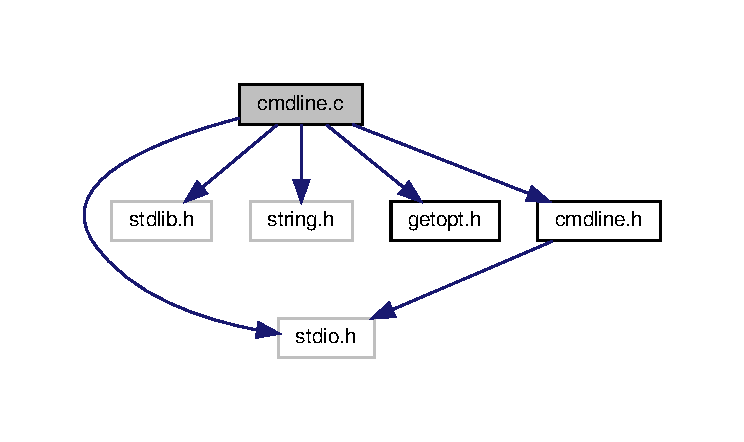
\includegraphics[width=350pt]{cmdline_8c__incl}
\end{center}
\end{figure}
\subsection*{Enumerations}
\begin{DoxyCompactItemize}
\item 
enum \hyperlink{cmdline_8c_a88e31a859f36efa57ad64e6ae13332a1}{cmdline\+\_\+parser\+\_\+arg\+\_\+type} \{ \newline
\hyperlink{cmdline_8c_a88e31a859f36efa57ad64e6ae13332a1a67dd250fb3e23862523b667407868ada}{A\+R\+G\+\_\+\+NO}, 
\hyperlink{cmdline_8c_a88e31a859f36efa57ad64e6ae13332a1afd135f03243c33991ef507f4410718f7}{A\+R\+G\+\_\+\+F\+L\+AG}, 
\hyperlink{cmdline_8c_a88e31a859f36efa57ad64e6ae13332a1a1e0904ee5e3baf2aa4070ab0718a3afa}{A\+R\+G\+\_\+\+S\+T\+R\+I\+NG}, 
\hyperlink{cmdline_8c_a88e31a859f36efa57ad64e6ae13332a1a58393752406d163205fa18f450909993}{A\+R\+G\+\_\+\+I\+NT}, 
\newline
\hyperlink{cmdline_8c_a88e31a859f36efa57ad64e6ae13332a1a5875de3e892eb32ed41e4d60ef7d99ca}{A\+R\+G\+\_\+\+F\+L\+O\+AT}
 \}
\end{DoxyCompactItemize}
\subsection*{Functions}
\begin{DoxyCompactItemize}
\item 
static void \hyperlink{cmdline_8c_a48968b912c47767e9f057f5bc11634cb}{clear\+\_\+given} (struct \hyperlink{structgengetopt__args__info}{gengetopt\+\_\+args\+\_\+info} $\ast$args\+\_\+info)
\item 
static void \hyperlink{cmdline_8c_a4d7018864f814395754ea4127ce4d37b}{clear\+\_\+args} (struct \hyperlink{structgengetopt__args__info}{gengetopt\+\_\+args\+\_\+info} $\ast$args\+\_\+info)
\item 
static int \hyperlink{cmdline_8c_aaba43e1bb216c68c96e982c600c906a7}{cmdline\+\_\+parser\+\_\+internal} (int argc, char $\ast$\hyperlink{getopt_8c_a2c212835823e3c54a8ab6d95c652660e}{const} $\ast$argv, struct \hyperlink{structgengetopt__args__info}{gengetopt\+\_\+args\+\_\+info} $\ast$args\+\_\+info, struct \hyperlink{structcmdline__parser__params}{cmdline\+\_\+parser\+\_\+params} $\ast$params, \hyperlink{getopt_8c_a2c212835823e3c54a8ab6d95c652660e}{const} char $\ast$additional\+\_\+error)
\item 
static char $\ast$ \hyperlink{cmdline_8c_a0ec9efd6eb3e6e939fcaaadd8b4c6a9f}{gengetopt\+\_\+strdup} (\hyperlink{getopt_8c_a2c212835823e3c54a8ab6d95c652660e}{const} char $\ast$s)
\begin{DoxyCompactList}\small\item\em replacement of strdup, which is not standard \end{DoxyCompactList}\item 
static void \hyperlink{cmdline_8c_a4dcfd361cdaac143739a02102296fedd}{init\+\_\+args\+\_\+info} (struct \hyperlink{structgengetopt__args__info}{gengetopt\+\_\+args\+\_\+info} $\ast$args\+\_\+info)
\item 
void \hyperlink{cmdline_8c_a96f27bf35ce0ab8eea7a1f6e6b59a5e2}{cmdline\+\_\+parser\+\_\+print\+\_\+version} (void)
\item 
static void \hyperlink{cmdline_8c_ad600bb9026825a295ea57df22bdf7eca}{print\+\_\+help\+\_\+common} (void)
\item 
void \hyperlink{cmdline_8c_ad4f7db2fa4002379eb30e5206f3b7492}{cmdline\+\_\+parser\+\_\+print\+\_\+help} (void)
\item 
void \hyperlink{cmdline_8c_aca62b50d03d0d082968eeb1940f98650}{cmdline\+\_\+parser\+\_\+init} (struct \hyperlink{structgengetopt__args__info}{gengetopt\+\_\+args\+\_\+info} $\ast$args\+\_\+info)
\item 
void \hyperlink{cmdline_8c_af72b814611cffc706b2135ccdfe7e997}{cmdline\+\_\+parser\+\_\+params\+\_\+init} (struct \hyperlink{structcmdline__parser__params}{cmdline\+\_\+parser\+\_\+params} $\ast$params)
\item 
struct \hyperlink{structcmdline__parser__params}{cmdline\+\_\+parser\+\_\+params} $\ast$ \hyperlink{cmdline_8c_afd778af110fe0ee1ea5eac7aa9939d92}{cmdline\+\_\+parser\+\_\+params\+\_\+create} (void)
\item 
static void \hyperlink{cmdline_8c_a3a3cc8b020811185cb0a4b96e1ff5a40}{free\+\_\+string\+\_\+field} (char $\ast$$\ast$s)
\item 
static void \hyperlink{cmdline_8c_ace6fb8241473bb89c5a575774eb4ba2a}{cmdline\+\_\+parser\+\_\+release} (struct \hyperlink{structgengetopt__args__info}{gengetopt\+\_\+args\+\_\+info} $\ast$args\+\_\+info)
\item 
static void \hyperlink{cmdline_8c_a332041b3060103618ef6b767ab32d0dd}{write\+\_\+into\+\_\+file} (F\+I\+LE $\ast$\hyperlink{postscript_8c_ae581849c67336453bd5b81e6518019a9}{outfile}, \hyperlink{getopt_8c_a2c212835823e3c54a8ab6d95c652660e}{const} char $\ast$opt, \hyperlink{getopt_8c_a2c212835823e3c54a8ab6d95c652660e}{const} char $\ast$arg, char $\ast$values\mbox{[}$\,$\mbox{]})
\item 
int \hyperlink{cmdline_8c_a1f73418092a6e6eb3706aa0de2785e11}{cmdline\+\_\+parser\+\_\+dump} (F\+I\+LE $\ast$\hyperlink{postscript_8c_ae581849c67336453bd5b81e6518019a9}{outfile}, struct \hyperlink{structgengetopt__args__info}{gengetopt\+\_\+args\+\_\+info} $\ast$args\+\_\+info)
\item 
int \hyperlink{cmdline_8c_a5f3e9412f88f1058a31ac28ad2ea2818}{cmdline\+\_\+parser\+\_\+file\+\_\+save} (\hyperlink{getopt_8c_a2c212835823e3c54a8ab6d95c652660e}{const} char $\ast$filename, struct \hyperlink{structgengetopt__args__info}{gengetopt\+\_\+args\+\_\+info} $\ast$args\+\_\+info)
\item 
void \hyperlink{cmdline_8c_af1b97c4e92b88f736e350b3902266ba4}{cmdline\+\_\+parser\+\_\+free} (struct \hyperlink{structgengetopt__args__info}{gengetopt\+\_\+args\+\_\+info} $\ast$args\+\_\+info)
\item 
int \hyperlink{cmdline_8c_a96f1044799c552f3ee139f9b1387b363}{cmdline\+\_\+parser} (int argc, char $\ast$\hyperlink{getopt_8c_a2c212835823e3c54a8ab6d95c652660e}{const} $\ast$argv, struct \hyperlink{structgengetopt__args__info}{gengetopt\+\_\+args\+\_\+info} $\ast$args\+\_\+info)
\item 
int \hyperlink{cmdline_8c_a77e461b5bdfd4a36c59a96bfb1813e38}{cmdline\+\_\+parser\+\_\+ext} (int argc, char $\ast$\hyperlink{getopt_8c_a2c212835823e3c54a8ab6d95c652660e}{const} $\ast$argv, struct \hyperlink{structgengetopt__args__info}{gengetopt\+\_\+args\+\_\+info} $\ast$args\+\_\+info, struct \hyperlink{structcmdline__parser__params}{cmdline\+\_\+parser\+\_\+params} $\ast$params)
\item 
int \hyperlink{cmdline_8c_a08e3536edc64ec5ee7c2df546c6e9dd7}{cmdline\+\_\+parser2} (int argc, char $\ast$\hyperlink{getopt_8c_a2c212835823e3c54a8ab6d95c652660e}{const} $\ast$argv, struct \hyperlink{structgengetopt__args__info}{gengetopt\+\_\+args\+\_\+info} $\ast$args\+\_\+info, int override, int initialize, int check\+\_\+required)
\item 
int \hyperlink{cmdline_8c_a83651e5be280d60aed58fdb72456a030}{cmdline\+\_\+parser\+\_\+required} (struct \hyperlink{structgengetopt__args__info}{gengetopt\+\_\+args\+\_\+info} $\ast$args\+\_\+info, \hyperlink{getopt_8c_a2c212835823e3c54a8ab6d95c652660e}{const} char $\ast$prog\+\_\+name)
\item 
static int \hyperlink{cmdline_8c_a21d8824d410efa489c4921011c1c0765}{update\+\_\+arg} (void $\ast$field, char $\ast$$\ast$orig\+\_\+field, unsigned int $\ast$field\+\_\+given, unsigned int $\ast$prev\+\_\+given, char $\ast$value, char $\ast$possible\+\_\+values\mbox{[}$\,$\mbox{]}, \hyperlink{getopt_8c_a2c212835823e3c54a8ab6d95c652660e}{const} char $\ast$default\+\_\+value, \hyperlink{cmdline_8c_a88e31a859f36efa57ad64e6ae13332a1}{cmdline\+\_\+parser\+\_\+arg\+\_\+type} arg\+\_\+type, int check\+\_\+ambiguity, int override, int no\+\_\+free, int multiple\+\_\+option, \hyperlink{getopt_8c_a2c212835823e3c54a8ab6d95c652660e}{const} char $\ast$long\+\_\+opt, char short\+\_\+opt, \hyperlink{getopt_8c_a2c212835823e3c54a8ab6d95c652660e}{const} char $\ast$additional\+\_\+error)
\begin{DoxyCompactList}\small\item\em updates an option \end{DoxyCompactList}\end{DoxyCompactItemize}
\subsection*{Variables}
\begin{DoxyCompactItemize}
\item 
\hyperlink{getopt_8c_a2c212835823e3c54a8ab6d95c652660e}{const} char $\ast$ \hyperlink{cmdline_8c_a610c3307abce5a8fd304b86b018ae60b}{gengetopt\+\_\+args\+\_\+info\+\_\+purpose} = \char`\"{}\char`\"{}
\begin{DoxyCompactList}\small\item\em the purpose string of the program \end{DoxyCompactList}\item 
\hyperlink{getopt_8c_a2c212835823e3c54a8ab6d95c652660e}{const} char $\ast$ \hyperlink{cmdline_8c_a9f397a306f363bfdebb611e86acf36d5}{gengetopt\+\_\+args\+\_\+info\+\_\+usage} = \char`\"{}Usage\+: \char`\"{} C\+M\+D\+L\+I\+N\+E\+\_\+\+P\+A\+R\+S\+E\+R\+\_\+\+P\+A\+C\+K\+A\+GE \char`\"{} \mbox{[}O\+P\+T\+I\+O\+NS\mbox{]}... \mbox{[}F\+I\+L\+ES\mbox{]}...\char`\"{}
\begin{DoxyCompactList}\small\item\em the usage string of the program \end{DoxyCompactList}\item 
\hyperlink{getopt_8c_a2c212835823e3c54a8ab6d95c652660e}{const} char $\ast$ \hyperlink{cmdline_8c_accad6107ca685f6eba555f6ce63d355d}{gengetopt\+\_\+args\+\_\+info\+\_\+description} = \char`\"{}\char`\"{}
\item 
\hyperlink{getopt_8c_a2c212835823e3c54a8ab6d95c652660e}{const} char $\ast$ \hyperlink{cmdline_8c_a6af7a6b7fb37c0abaa916ee1cfa0a41f}{gengetopt\+\_\+args\+\_\+info\+\_\+help} \mbox{[}$\,$\mbox{]}
\begin{DoxyCompactList}\small\item\em all the lines making the help output \end{DoxyCompactList}\item 
static char $\ast$ \hyperlink{cmdline_8c_a08f16a026de44b77c5e7be490fb9e32b}{package\+\_\+name} = 0
\end{DoxyCompactItemize}


\subsection{Enumeration Type Documentation}
\mbox{\Hypertarget{cmdline_8c_a88e31a859f36efa57ad64e6ae13332a1}\label{cmdline_8c_a88e31a859f36efa57ad64e6ae13332a1}} 
\index{cmdline.\+c@{cmdline.\+c}!cmdline\+\_\+parser\+\_\+arg\+\_\+type@{cmdline\+\_\+parser\+\_\+arg\+\_\+type}}
\index{cmdline\+\_\+parser\+\_\+arg\+\_\+type@{cmdline\+\_\+parser\+\_\+arg\+\_\+type}!cmdline.\+c@{cmdline.\+c}}
\subsubsection{\texorpdfstring{cmdline\+\_\+parser\+\_\+arg\+\_\+type}{cmdline\_parser\_arg\_type}}
{\footnotesize\ttfamily enum \hyperlink{cmdline_8c_a88e31a859f36efa57ad64e6ae13332a1}{cmdline\+\_\+parser\+\_\+arg\+\_\+type}}

\begin{DoxyEnumFields}{Enumerator}
\raisebox{\heightof{T}}[0pt][0pt]{\index{A\+R\+G\+\_\+\+NO@{A\+R\+G\+\_\+\+NO}!cmdline.\+c@{cmdline.\+c}}\index{cmdline.\+c@{cmdline.\+c}!A\+R\+G\+\_\+\+NO@{A\+R\+G\+\_\+\+NO}}}\mbox{\Hypertarget{cmdline_8c_a88e31a859f36efa57ad64e6ae13332a1a67dd250fb3e23862523b667407868ada}\label{cmdline_8c_a88e31a859f36efa57ad64e6ae13332a1a67dd250fb3e23862523b667407868ada}} 
A\+R\+G\+\_\+\+NO&\\
\hline

\raisebox{\heightof{T}}[0pt][0pt]{\index{A\+R\+G\+\_\+\+F\+L\+AG@{A\+R\+G\+\_\+\+F\+L\+AG}!cmdline.\+c@{cmdline.\+c}}\index{cmdline.\+c@{cmdline.\+c}!A\+R\+G\+\_\+\+F\+L\+AG@{A\+R\+G\+\_\+\+F\+L\+AG}}}\mbox{\Hypertarget{cmdline_8c_a88e31a859f36efa57ad64e6ae13332a1afd135f03243c33991ef507f4410718f7}\label{cmdline_8c_a88e31a859f36efa57ad64e6ae13332a1afd135f03243c33991ef507f4410718f7}} 
A\+R\+G\+\_\+\+F\+L\+AG&\\
\hline

\raisebox{\heightof{T}}[0pt][0pt]{\index{A\+R\+G\+\_\+\+S\+T\+R\+I\+NG@{A\+R\+G\+\_\+\+S\+T\+R\+I\+NG}!cmdline.\+c@{cmdline.\+c}}\index{cmdline.\+c@{cmdline.\+c}!A\+R\+G\+\_\+\+S\+T\+R\+I\+NG@{A\+R\+G\+\_\+\+S\+T\+R\+I\+NG}}}\mbox{\Hypertarget{cmdline_8c_a88e31a859f36efa57ad64e6ae13332a1a1e0904ee5e3baf2aa4070ab0718a3afa}\label{cmdline_8c_a88e31a859f36efa57ad64e6ae13332a1a1e0904ee5e3baf2aa4070ab0718a3afa}} 
A\+R\+G\+\_\+\+S\+T\+R\+I\+NG&\\
\hline

\raisebox{\heightof{T}}[0pt][0pt]{\index{A\+R\+G\+\_\+\+I\+NT@{A\+R\+G\+\_\+\+I\+NT}!cmdline.\+c@{cmdline.\+c}}\index{cmdline.\+c@{cmdline.\+c}!A\+R\+G\+\_\+\+I\+NT@{A\+R\+G\+\_\+\+I\+NT}}}\mbox{\Hypertarget{cmdline_8c_a88e31a859f36efa57ad64e6ae13332a1a58393752406d163205fa18f450909993}\label{cmdline_8c_a88e31a859f36efa57ad64e6ae13332a1a58393752406d163205fa18f450909993}} 
A\+R\+G\+\_\+\+I\+NT&\\
\hline

\raisebox{\heightof{T}}[0pt][0pt]{\index{A\+R\+G\+\_\+\+F\+L\+O\+AT@{A\+R\+G\+\_\+\+F\+L\+O\+AT}!cmdline.\+c@{cmdline.\+c}}\index{cmdline.\+c@{cmdline.\+c}!A\+R\+G\+\_\+\+F\+L\+O\+AT@{A\+R\+G\+\_\+\+F\+L\+O\+AT}}}\mbox{\Hypertarget{cmdline_8c_a88e31a859f36efa57ad64e6ae13332a1a5875de3e892eb32ed41e4d60ef7d99ca}\label{cmdline_8c_a88e31a859f36efa57ad64e6ae13332a1a5875de3e892eb32ed41e4d60ef7d99ca}} 
A\+R\+G\+\_\+\+F\+L\+O\+AT&\\
\hline

\end{DoxyEnumFields}


\subsection{Function Documentation}
\mbox{\Hypertarget{cmdline_8c_a4d7018864f814395754ea4127ce4d37b}\label{cmdline_8c_a4d7018864f814395754ea4127ce4d37b}} 
\index{cmdline.\+c@{cmdline.\+c}!clear\+\_\+args@{clear\+\_\+args}}
\index{clear\+\_\+args@{clear\+\_\+args}!cmdline.\+c@{cmdline.\+c}}
\subsubsection{\texorpdfstring{clear\+\_\+args()}{clear\_args()}}
{\footnotesize\ttfamily static void clear\+\_\+args (\begin{DoxyParamCaption}\item[{struct \hyperlink{structgengetopt__args__info}{gengetopt\+\_\+args\+\_\+info} $\ast$}]{args\+\_\+info }\end{DoxyParamCaption})\hspace{0.3cm}{\ttfamily [static]}}

\mbox{\Hypertarget{cmdline_8c_a48968b912c47767e9f057f5bc11634cb}\label{cmdline_8c_a48968b912c47767e9f057f5bc11634cb}} 
\index{cmdline.\+c@{cmdline.\+c}!clear\+\_\+given@{clear\+\_\+given}}
\index{clear\+\_\+given@{clear\+\_\+given}!cmdline.\+c@{cmdline.\+c}}
\subsubsection{\texorpdfstring{clear\+\_\+given()}{clear\_given()}}
{\footnotesize\ttfamily static void clear\+\_\+given (\begin{DoxyParamCaption}\item[{struct \hyperlink{structgengetopt__args__info}{gengetopt\+\_\+args\+\_\+info} $\ast$}]{args\+\_\+info }\end{DoxyParamCaption})\hspace{0.3cm}{\ttfamily [static]}}

\mbox{\Hypertarget{cmdline_8c_a96f1044799c552f3ee139f9b1387b363}\label{cmdline_8c_a96f1044799c552f3ee139f9b1387b363}} 
\index{cmdline.\+c@{cmdline.\+c}!cmdline\+\_\+parser@{cmdline\+\_\+parser}}
\index{cmdline\+\_\+parser@{cmdline\+\_\+parser}!cmdline.\+c@{cmdline.\+c}}
\subsubsection{\texorpdfstring{cmdline\+\_\+parser()}{cmdline\_parser()}}
{\footnotesize\ttfamily int cmdline\+\_\+parser (\begin{DoxyParamCaption}\item[{int}]{argc,  }\item[{char $\ast$\hyperlink{getopt_8c_a2c212835823e3c54a8ab6d95c652660e}{const} $\ast$}]{argv,  }\item[{struct \hyperlink{structgengetopt__args__info}{gengetopt\+\_\+args\+\_\+info} $\ast$}]{args\+\_\+info }\end{DoxyParamCaption})}

The command line parser 
\begin{DoxyParams}{Parameters}
{\em argc} & the number of command line options \\
\hline
{\em argv} & the command line options \\
\hline
{\em args\+\_\+info} & the structure where option information will be stored \\
\hline
\end{DoxyParams}
\begin{DoxyReturn}{Returns}
0 if everything went fine, N\+ON 0 if an error took place 
\end{DoxyReturn}
Here is the call graph for this function\+:
\nopagebreak
\begin{figure}[H]
\begin{center}
\leavevmode
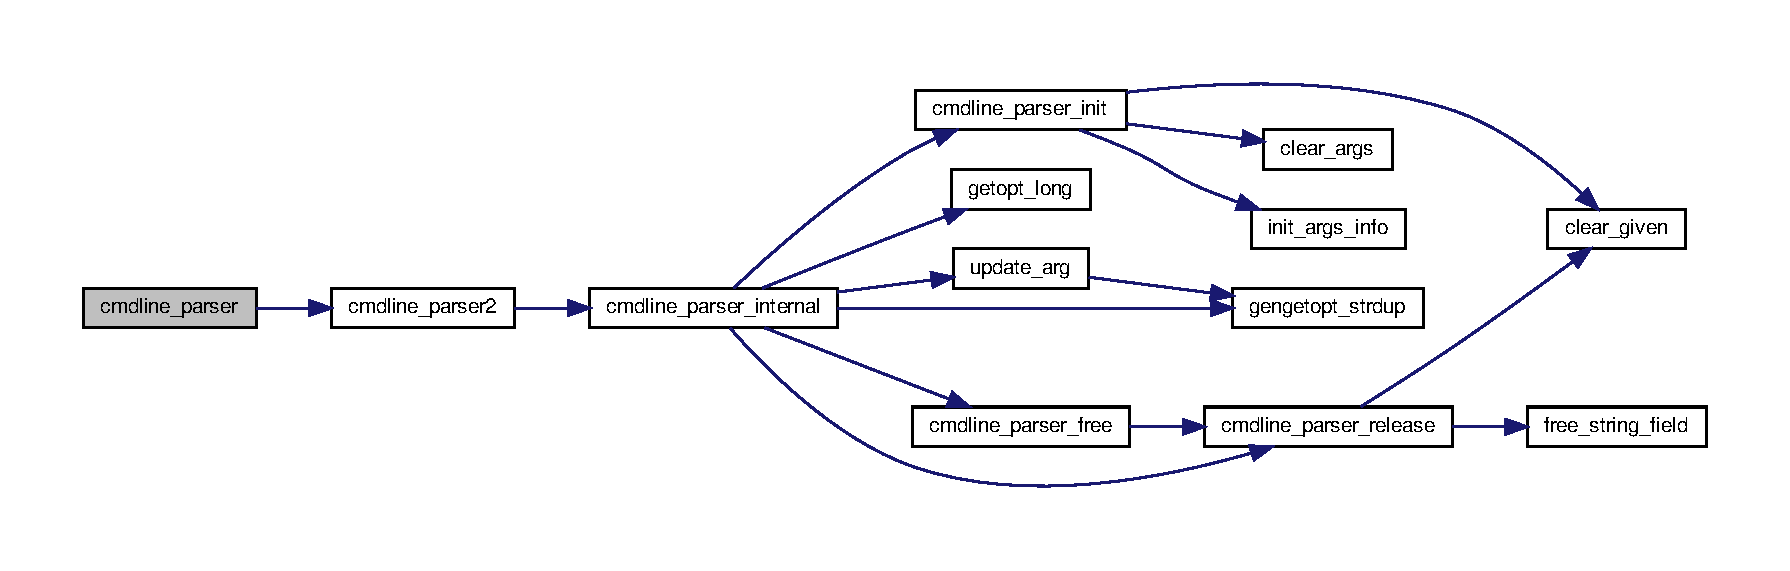
\includegraphics[width=350pt]{cmdline_8c_a96f1044799c552f3ee139f9b1387b363_cgraph}
\end{center}
\end{figure}
\mbox{\Hypertarget{cmdline_8c_a08e3536edc64ec5ee7c2df546c6e9dd7}\label{cmdline_8c_a08e3536edc64ec5ee7c2df546c6e9dd7}} 
\index{cmdline.\+c@{cmdline.\+c}!cmdline\+\_\+parser2@{cmdline\+\_\+parser2}}
\index{cmdline\+\_\+parser2@{cmdline\+\_\+parser2}!cmdline.\+c@{cmdline.\+c}}
\subsubsection{\texorpdfstring{cmdline\+\_\+parser2()}{cmdline\_parser2()}}
{\footnotesize\ttfamily int cmdline\+\_\+parser2 (\begin{DoxyParamCaption}\item[{int}]{argc,  }\item[{char $\ast$\hyperlink{getopt_8c_a2c212835823e3c54a8ab6d95c652660e}{const} $\ast$}]{argv,  }\item[{struct \hyperlink{structgengetopt__args__info}{gengetopt\+\_\+args\+\_\+info} $\ast$}]{args\+\_\+info,  }\item[{int}]{override,  }\item[{int}]{initialize,  }\item[{int}]{check\+\_\+required }\end{DoxyParamCaption})}

The command line parser (version with additional parameters -\/ deprecated) 
\begin{DoxyParams}{Parameters}
{\em argc} & the number of command line options \\
\hline
{\em argv} & the command line options \\
\hline
{\em args\+\_\+info} & the structure where option information will be stored \\
\hline
{\em override} & whether to override possibly already present options \\
\hline
{\em initialize} & whether to initialize the option structure my\+\_\+args\+\_\+info \\
\hline
{\em check\+\_\+required} & whether to check that all required options were provided \\
\hline
\end{DoxyParams}
\begin{DoxyReturn}{Returns}
0 if everything went fine, N\+ON 0 if an error took place 
\end{DoxyReturn}
\begin{DoxyRefDesc}{Deprecated}
\item[\hyperlink{deprecated__deprecated000001}{Deprecated}]use \hyperlink{cmdline_8h_a77e461b5bdfd4a36c59a96bfb1813e38}{cmdline\+\_\+parser\+\_\+ext()} instead \end{DoxyRefDesc}
Here is the call graph for this function\+:
\nopagebreak
\begin{figure}[H]
\begin{center}
\leavevmode
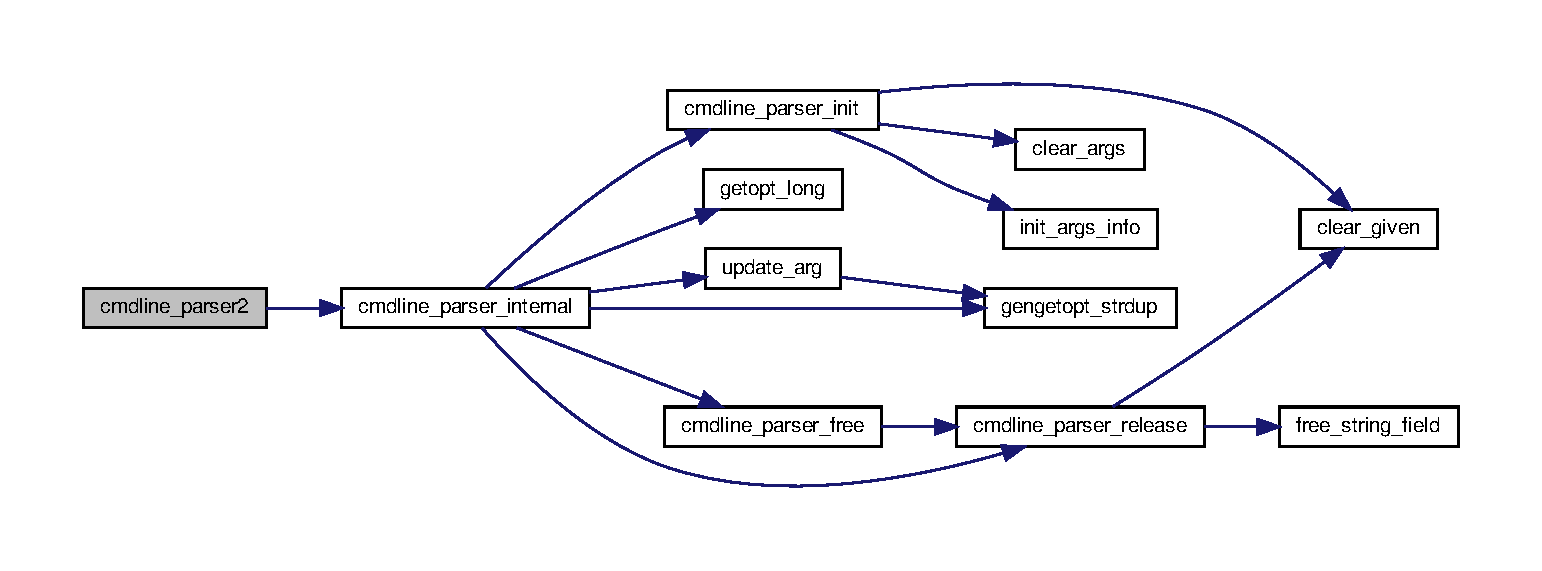
\includegraphics[width=350pt]{cmdline_8c_a08e3536edc64ec5ee7c2df546c6e9dd7_cgraph}
\end{center}
\end{figure}
\mbox{\Hypertarget{cmdline_8c_a1f73418092a6e6eb3706aa0de2785e11}\label{cmdline_8c_a1f73418092a6e6eb3706aa0de2785e11}} 
\index{cmdline.\+c@{cmdline.\+c}!cmdline\+\_\+parser\+\_\+dump@{cmdline\+\_\+parser\+\_\+dump}}
\index{cmdline\+\_\+parser\+\_\+dump@{cmdline\+\_\+parser\+\_\+dump}!cmdline.\+c@{cmdline.\+c}}
\subsubsection{\texorpdfstring{cmdline\+\_\+parser\+\_\+dump()}{cmdline\_parser\_dump()}}
{\footnotesize\ttfamily int cmdline\+\_\+parser\+\_\+dump (\begin{DoxyParamCaption}\item[{F\+I\+LE $\ast$}]{outfile,  }\item[{struct \hyperlink{structgengetopt__args__info}{gengetopt\+\_\+args\+\_\+info} $\ast$}]{args\+\_\+info }\end{DoxyParamCaption})}

Save the contents of the option struct into an already open F\+I\+LE stream. 
\begin{DoxyParams}{Parameters}
{\em outfile} & the stream where to dump options \\
\hline
{\em args\+\_\+info} & the option struct to dump \\
\hline
\end{DoxyParams}
\begin{DoxyReturn}{Returns}
0 if everything went fine, N\+ON 0 if an error took place 
\end{DoxyReturn}
Here is the call graph for this function\+:
\nopagebreak
\begin{figure}[H]
\begin{center}
\leavevmode
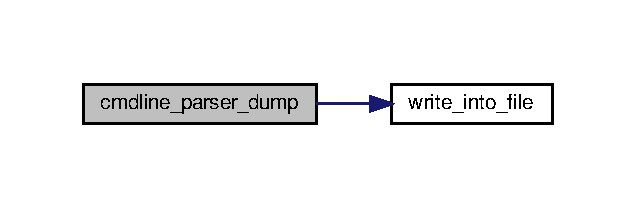
\includegraphics[width=305pt]{cmdline_8c_a1f73418092a6e6eb3706aa0de2785e11_cgraph}
\end{center}
\end{figure}
\mbox{\Hypertarget{cmdline_8c_a77e461b5bdfd4a36c59a96bfb1813e38}\label{cmdline_8c_a77e461b5bdfd4a36c59a96bfb1813e38}} 
\index{cmdline.\+c@{cmdline.\+c}!cmdline\+\_\+parser\+\_\+ext@{cmdline\+\_\+parser\+\_\+ext}}
\index{cmdline\+\_\+parser\+\_\+ext@{cmdline\+\_\+parser\+\_\+ext}!cmdline.\+c@{cmdline.\+c}}
\subsubsection{\texorpdfstring{cmdline\+\_\+parser\+\_\+ext()}{cmdline\_parser\_ext()}}
{\footnotesize\ttfamily int cmdline\+\_\+parser\+\_\+ext (\begin{DoxyParamCaption}\item[{int}]{argc,  }\item[{char $\ast$\hyperlink{getopt_8c_a2c212835823e3c54a8ab6d95c652660e}{const} $\ast$}]{argv,  }\item[{struct \hyperlink{structgengetopt__args__info}{gengetopt\+\_\+args\+\_\+info} $\ast$}]{args\+\_\+info,  }\item[{struct \hyperlink{structcmdline__parser__params}{cmdline\+\_\+parser\+\_\+params} $\ast$}]{params }\end{DoxyParamCaption})}

The command line parser (version with additional parameters) 
\begin{DoxyParams}{Parameters}
{\em argc} & the number of command line options \\
\hline
{\em argv} & the command line options \\
\hline
{\em args\+\_\+info} & the structure where option information will be stored \\
\hline
{\em params} & additional parameters for the parser \\
\hline
\end{DoxyParams}
\begin{DoxyReturn}{Returns}
0 if everything went fine, N\+ON 0 if an error took place 
\end{DoxyReturn}
Here is the call graph for this function\+:
\nopagebreak
\begin{figure}[H]
\begin{center}
\leavevmode
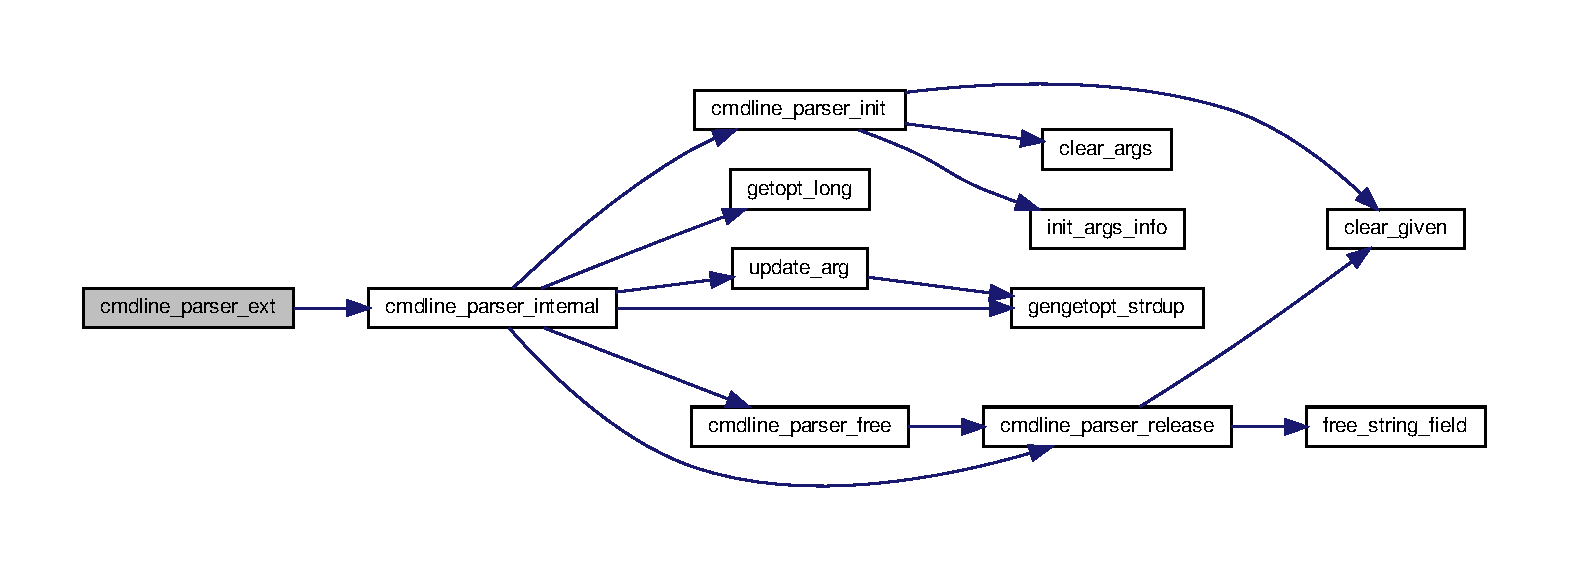
\includegraphics[width=350pt]{cmdline_8c_a77e461b5bdfd4a36c59a96bfb1813e38_cgraph}
\end{center}
\end{figure}
\mbox{\Hypertarget{cmdline_8c_a5f3e9412f88f1058a31ac28ad2ea2818}\label{cmdline_8c_a5f3e9412f88f1058a31ac28ad2ea2818}} 
\index{cmdline.\+c@{cmdline.\+c}!cmdline\+\_\+parser\+\_\+file\+\_\+save@{cmdline\+\_\+parser\+\_\+file\+\_\+save}}
\index{cmdline\+\_\+parser\+\_\+file\+\_\+save@{cmdline\+\_\+parser\+\_\+file\+\_\+save}!cmdline.\+c@{cmdline.\+c}}
\subsubsection{\texorpdfstring{cmdline\+\_\+parser\+\_\+file\+\_\+save()}{cmdline\_parser\_file\_save()}}
{\footnotesize\ttfamily int cmdline\+\_\+parser\+\_\+file\+\_\+save (\begin{DoxyParamCaption}\item[{\hyperlink{getopt_8c_a2c212835823e3c54a8ab6d95c652660e}{const} char $\ast$}]{filename,  }\item[{struct \hyperlink{structgengetopt__args__info}{gengetopt\+\_\+args\+\_\+info} $\ast$}]{args\+\_\+info }\end{DoxyParamCaption})}

Save the contents of the option struct into a (text) file. This file can be read by the config file parser (if generated by gengetopt) 
\begin{DoxyParams}{Parameters}
{\em filename} & the file where to save \\
\hline
{\em args\+\_\+info} & the option struct to save \\
\hline
\end{DoxyParams}
\begin{DoxyReturn}{Returns}
0 if everything went fine, N\+ON 0 if an error took place 
\end{DoxyReturn}
Here is the call graph for this function\+:
\nopagebreak
\begin{figure}[H]
\begin{center}
\leavevmode
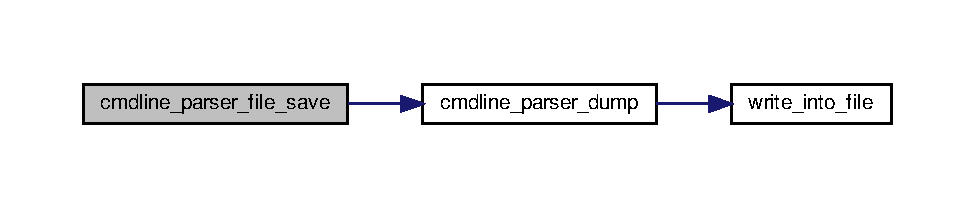
\includegraphics[width=350pt]{cmdline_8c_a5f3e9412f88f1058a31ac28ad2ea2818_cgraph}
\end{center}
\end{figure}
\mbox{\Hypertarget{cmdline_8c_af1b97c4e92b88f736e350b3902266ba4}\label{cmdline_8c_af1b97c4e92b88f736e350b3902266ba4}} 
\index{cmdline.\+c@{cmdline.\+c}!cmdline\+\_\+parser\+\_\+free@{cmdline\+\_\+parser\+\_\+free}}
\index{cmdline\+\_\+parser\+\_\+free@{cmdline\+\_\+parser\+\_\+free}!cmdline.\+c@{cmdline.\+c}}
\subsubsection{\texorpdfstring{cmdline\+\_\+parser\+\_\+free()}{cmdline\_parser\_free()}}
{\footnotesize\ttfamily void cmdline\+\_\+parser\+\_\+free (\begin{DoxyParamCaption}\item[{struct \hyperlink{structgengetopt__args__info}{gengetopt\+\_\+args\+\_\+info} $\ast$}]{args\+\_\+info }\end{DoxyParamCaption})}

Deallocates the string fields of the \hyperlink{structgengetopt__args__info}{gengetopt\+\_\+args\+\_\+info} structure (but does not deallocate the structure itself) 
\begin{DoxyParams}{Parameters}
{\em args\+\_\+info} & the structure to deallocate \\
\hline
\end{DoxyParams}
Here is the call graph for this function\+:
\nopagebreak
\begin{figure}[H]
\begin{center}
\leavevmode
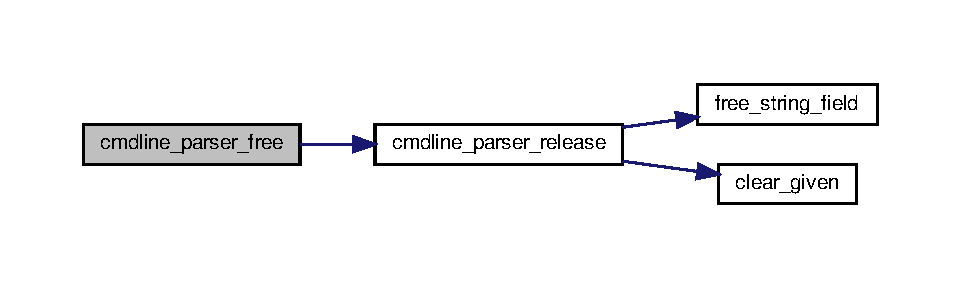
\includegraphics[width=350pt]{cmdline_8c_af1b97c4e92b88f736e350b3902266ba4_cgraph}
\end{center}
\end{figure}
\mbox{\Hypertarget{cmdline_8c_aca62b50d03d0d082968eeb1940f98650}\label{cmdline_8c_aca62b50d03d0d082968eeb1940f98650}} 
\index{cmdline.\+c@{cmdline.\+c}!cmdline\+\_\+parser\+\_\+init@{cmdline\+\_\+parser\+\_\+init}}
\index{cmdline\+\_\+parser\+\_\+init@{cmdline\+\_\+parser\+\_\+init}!cmdline.\+c@{cmdline.\+c}}
\subsubsection{\texorpdfstring{cmdline\+\_\+parser\+\_\+init()}{cmdline\_parser\_init()}}
{\footnotesize\ttfamily void cmdline\+\_\+parser\+\_\+init (\begin{DoxyParamCaption}\item[{struct \hyperlink{structgengetopt__args__info}{gengetopt\+\_\+args\+\_\+info} $\ast$}]{args\+\_\+info }\end{DoxyParamCaption})}

Initializes the passed \hyperlink{structgengetopt__args__info}{gengetopt\+\_\+args\+\_\+info} structure\textquotesingle{}s fields (also set default values for options that have a default) 
\begin{DoxyParams}{Parameters}
{\em args\+\_\+info} & the structure to initialize \\
\hline
\end{DoxyParams}
Here is the call graph for this function\+:
\nopagebreak
\begin{figure}[H]
\begin{center}
\leavevmode
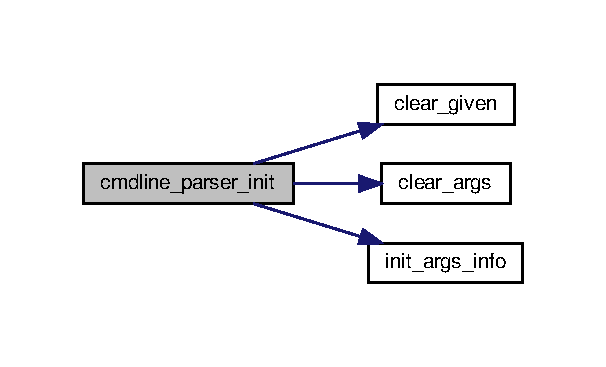
\includegraphics[width=291pt]{cmdline_8c_aca62b50d03d0d082968eeb1940f98650_cgraph}
\end{center}
\end{figure}
\mbox{\Hypertarget{cmdline_8c_aaba43e1bb216c68c96e982c600c906a7}\label{cmdline_8c_aaba43e1bb216c68c96e982c600c906a7}} 
\index{cmdline.\+c@{cmdline.\+c}!cmdline\+\_\+parser\+\_\+internal@{cmdline\+\_\+parser\+\_\+internal}}
\index{cmdline\+\_\+parser\+\_\+internal@{cmdline\+\_\+parser\+\_\+internal}!cmdline.\+c@{cmdline.\+c}}
\subsubsection{\texorpdfstring{cmdline\+\_\+parser\+\_\+internal()}{cmdline\_parser\_internal()}}
{\footnotesize\ttfamily int cmdline\+\_\+parser\+\_\+internal (\begin{DoxyParamCaption}\item[{int}]{argc,  }\item[{char $\ast$\hyperlink{getopt_8c_a2c212835823e3c54a8ab6d95c652660e}{const} $\ast$}]{argv,  }\item[{struct \hyperlink{structgengetopt__args__info}{gengetopt\+\_\+args\+\_\+info} $\ast$}]{args\+\_\+info,  }\item[{struct \hyperlink{structcmdline__parser__params}{cmdline\+\_\+parser\+\_\+params} $\ast$}]{params,  }\item[{\hyperlink{getopt_8c_a2c212835823e3c54a8ab6d95c652660e}{const} char $\ast$}]{additional\+\_\+error }\end{DoxyParamCaption})\hspace{0.3cm}{\ttfamily [static]}}

Here is the call graph for this function\+:
\nopagebreak
\begin{figure}[H]
\begin{center}
\leavevmode
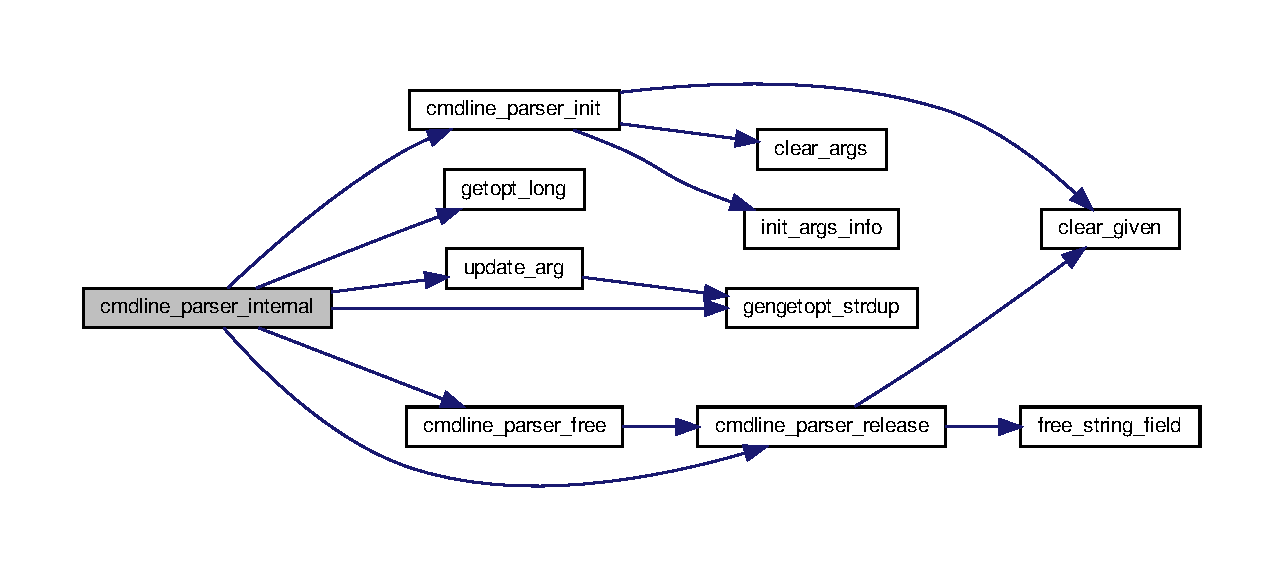
\includegraphics[width=350pt]{cmdline_8c_aaba43e1bb216c68c96e982c600c906a7_cgraph}
\end{center}
\end{figure}
\mbox{\Hypertarget{cmdline_8c_afd778af110fe0ee1ea5eac7aa9939d92}\label{cmdline_8c_afd778af110fe0ee1ea5eac7aa9939d92}} 
\index{cmdline.\+c@{cmdline.\+c}!cmdline\+\_\+parser\+\_\+params\+\_\+create@{cmdline\+\_\+parser\+\_\+params\+\_\+create}}
\index{cmdline\+\_\+parser\+\_\+params\+\_\+create@{cmdline\+\_\+parser\+\_\+params\+\_\+create}!cmdline.\+c@{cmdline.\+c}}
\subsubsection{\texorpdfstring{cmdline\+\_\+parser\+\_\+params\+\_\+create()}{cmdline\_parser\_params\_create()}}
{\footnotesize\ttfamily struct \hyperlink{structcmdline__parser__params}{cmdline\+\_\+parser\+\_\+params}$\ast$ cmdline\+\_\+parser\+\_\+params\+\_\+create (\begin{DoxyParamCaption}\item[{void}]{ }\end{DoxyParamCaption})}

Allocates dynamically a \hyperlink{structcmdline__parser__params}{cmdline\+\_\+parser\+\_\+params} structure and initializes all its fields to their default values \begin{DoxyReturn}{Returns}
the created and initialized \hyperlink{structcmdline__parser__params}{cmdline\+\_\+parser\+\_\+params} structure 
\end{DoxyReturn}
Here is the call graph for this function\+:
\nopagebreak
\begin{figure}[H]
\begin{center}
\leavevmode
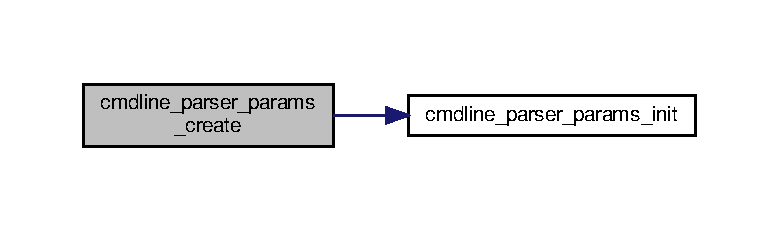
\includegraphics[width=350pt]{cmdline_8c_afd778af110fe0ee1ea5eac7aa9939d92_cgraph}
\end{center}
\end{figure}
\mbox{\Hypertarget{cmdline_8c_af72b814611cffc706b2135ccdfe7e997}\label{cmdline_8c_af72b814611cffc706b2135ccdfe7e997}} 
\index{cmdline.\+c@{cmdline.\+c}!cmdline\+\_\+parser\+\_\+params\+\_\+init@{cmdline\+\_\+parser\+\_\+params\+\_\+init}}
\index{cmdline\+\_\+parser\+\_\+params\+\_\+init@{cmdline\+\_\+parser\+\_\+params\+\_\+init}!cmdline.\+c@{cmdline.\+c}}
\subsubsection{\texorpdfstring{cmdline\+\_\+parser\+\_\+params\+\_\+init()}{cmdline\_parser\_params\_init()}}
{\footnotesize\ttfamily void cmdline\+\_\+parser\+\_\+params\+\_\+init (\begin{DoxyParamCaption}\item[{struct \hyperlink{structcmdline__parser__params}{cmdline\+\_\+parser\+\_\+params} $\ast$}]{params }\end{DoxyParamCaption})}

Initializes all the fields a \hyperlink{structcmdline__parser__params}{cmdline\+\_\+parser\+\_\+params} structure to their default values 
\begin{DoxyParams}{Parameters}
{\em params} & the structure to initialize \\
\hline
\end{DoxyParams}
\mbox{\Hypertarget{cmdline_8c_ad4f7db2fa4002379eb30e5206f3b7492}\label{cmdline_8c_ad4f7db2fa4002379eb30e5206f3b7492}} 
\index{cmdline.\+c@{cmdline.\+c}!cmdline\+\_\+parser\+\_\+print\+\_\+help@{cmdline\+\_\+parser\+\_\+print\+\_\+help}}
\index{cmdline\+\_\+parser\+\_\+print\+\_\+help@{cmdline\+\_\+parser\+\_\+print\+\_\+help}!cmdline.\+c@{cmdline.\+c}}
\subsubsection{\texorpdfstring{cmdline\+\_\+parser\+\_\+print\+\_\+help()}{cmdline\_parser\_print\_help()}}
{\footnotesize\ttfamily void cmdline\+\_\+parser\+\_\+print\+\_\+help (\begin{DoxyParamCaption}\item[{void}]{ }\end{DoxyParamCaption})}

Print the help Here is the call graph for this function\+:
\nopagebreak
\begin{figure}[H]
\begin{center}
\leavevmode
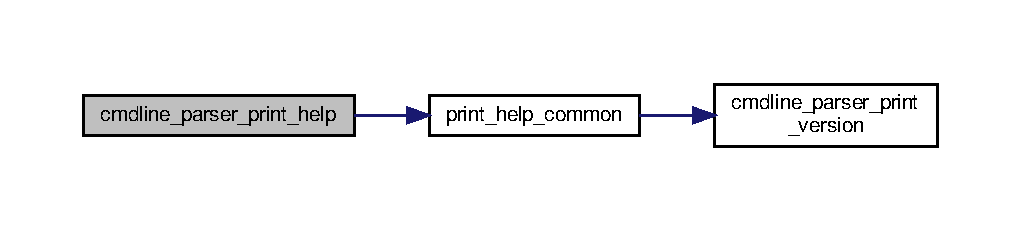
\includegraphics[width=350pt]{cmdline_8c_ad4f7db2fa4002379eb30e5206f3b7492_cgraph}
\end{center}
\end{figure}
\mbox{\Hypertarget{cmdline_8c_a96f27bf35ce0ab8eea7a1f6e6b59a5e2}\label{cmdline_8c_a96f27bf35ce0ab8eea7a1f6e6b59a5e2}} 
\index{cmdline.\+c@{cmdline.\+c}!cmdline\+\_\+parser\+\_\+print\+\_\+version@{cmdline\+\_\+parser\+\_\+print\+\_\+version}}
\index{cmdline\+\_\+parser\+\_\+print\+\_\+version@{cmdline\+\_\+parser\+\_\+print\+\_\+version}!cmdline.\+c@{cmdline.\+c}}
\subsubsection{\texorpdfstring{cmdline\+\_\+parser\+\_\+print\+\_\+version()}{cmdline\_parser\_print\_version()}}
{\footnotesize\ttfamily void cmdline\+\_\+parser\+\_\+print\+\_\+version (\begin{DoxyParamCaption}\item[{void}]{ }\end{DoxyParamCaption})}

Print the version \mbox{\Hypertarget{cmdline_8c_ace6fb8241473bb89c5a575774eb4ba2a}\label{cmdline_8c_ace6fb8241473bb89c5a575774eb4ba2a}} 
\index{cmdline.\+c@{cmdline.\+c}!cmdline\+\_\+parser\+\_\+release@{cmdline\+\_\+parser\+\_\+release}}
\index{cmdline\+\_\+parser\+\_\+release@{cmdline\+\_\+parser\+\_\+release}!cmdline.\+c@{cmdline.\+c}}
\subsubsection{\texorpdfstring{cmdline\+\_\+parser\+\_\+release()}{cmdline\_parser\_release()}}
{\footnotesize\ttfamily static void cmdline\+\_\+parser\+\_\+release (\begin{DoxyParamCaption}\item[{struct \hyperlink{structgengetopt__args__info}{gengetopt\+\_\+args\+\_\+info} $\ast$}]{args\+\_\+info }\end{DoxyParamCaption})\hspace{0.3cm}{\ttfamily [static]}}

Here is the call graph for this function\+:
\nopagebreak
\begin{figure}[H]
\begin{center}
\leavevmode
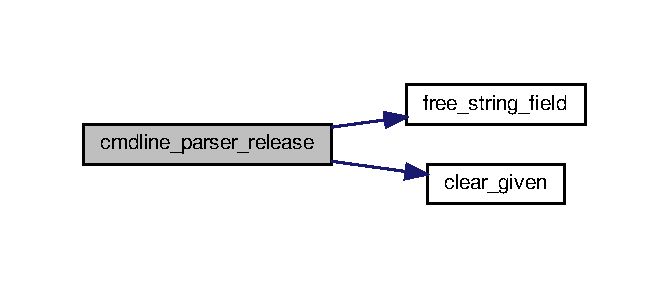
\includegraphics[width=321pt]{cmdline_8c_ace6fb8241473bb89c5a575774eb4ba2a_cgraph}
\end{center}
\end{figure}
\mbox{\Hypertarget{cmdline_8c_a83651e5be280d60aed58fdb72456a030}\label{cmdline_8c_a83651e5be280d60aed58fdb72456a030}} 
\index{cmdline.\+c@{cmdline.\+c}!cmdline\+\_\+parser\+\_\+required@{cmdline\+\_\+parser\+\_\+required}}
\index{cmdline\+\_\+parser\+\_\+required@{cmdline\+\_\+parser\+\_\+required}!cmdline.\+c@{cmdline.\+c}}
\subsubsection{\texorpdfstring{cmdline\+\_\+parser\+\_\+required()}{cmdline\_parser\_required()}}
{\footnotesize\ttfamily int cmdline\+\_\+parser\+\_\+required (\begin{DoxyParamCaption}\item[{struct \hyperlink{structgengetopt__args__info}{gengetopt\+\_\+args\+\_\+info} $\ast$}]{args\+\_\+info,  }\item[{\hyperlink{getopt_8c_a2c212835823e3c54a8ab6d95c652660e}{const} char $\ast$}]{prog\+\_\+name }\end{DoxyParamCaption})}

Checks that all the required options were specified 
\begin{DoxyParams}{Parameters}
{\em args\+\_\+info} & the structure to check \\
\hline
{\em prog\+\_\+name} & the name of the program that will be used to print possible errors \\
\hline
\end{DoxyParams}
\begin{DoxyReturn}{Returns}

\end{DoxyReturn}
\mbox{\Hypertarget{cmdline_8c_a3a3cc8b020811185cb0a4b96e1ff5a40}\label{cmdline_8c_a3a3cc8b020811185cb0a4b96e1ff5a40}} 
\index{cmdline.\+c@{cmdline.\+c}!free\+\_\+string\+\_\+field@{free\+\_\+string\+\_\+field}}
\index{free\+\_\+string\+\_\+field@{free\+\_\+string\+\_\+field}!cmdline.\+c@{cmdline.\+c}}
\subsubsection{\texorpdfstring{free\+\_\+string\+\_\+field()}{free\_string\_field()}}
{\footnotesize\ttfamily static void free\+\_\+string\+\_\+field (\begin{DoxyParamCaption}\item[{char $\ast$$\ast$}]{s }\end{DoxyParamCaption})\hspace{0.3cm}{\ttfamily [static]}}

\mbox{\Hypertarget{cmdline_8c_a0ec9efd6eb3e6e939fcaaadd8b4c6a9f}\label{cmdline_8c_a0ec9efd6eb3e6e939fcaaadd8b4c6a9f}} 
\index{cmdline.\+c@{cmdline.\+c}!gengetopt\+\_\+strdup@{gengetopt\+\_\+strdup}}
\index{gengetopt\+\_\+strdup@{gengetopt\+\_\+strdup}!cmdline.\+c@{cmdline.\+c}}
\subsubsection{\texorpdfstring{gengetopt\+\_\+strdup()}{gengetopt\_strdup()}}
{\footnotesize\ttfamily char $\ast$ gengetopt\+\_\+strdup (\begin{DoxyParamCaption}\item[{\hyperlink{getopt_8c_a2c212835823e3c54a8ab6d95c652660e}{const} char $\ast$}]{s }\end{DoxyParamCaption})\hspace{0.3cm}{\ttfamily [static]}}



replacement of strdup, which is not standard 

\mbox{\Hypertarget{cmdline_8c_a4dcfd361cdaac143739a02102296fedd}\label{cmdline_8c_a4dcfd361cdaac143739a02102296fedd}} 
\index{cmdline.\+c@{cmdline.\+c}!init\+\_\+args\+\_\+info@{init\+\_\+args\+\_\+info}}
\index{init\+\_\+args\+\_\+info@{init\+\_\+args\+\_\+info}!cmdline.\+c@{cmdline.\+c}}
\subsubsection{\texorpdfstring{init\+\_\+args\+\_\+info()}{init\_args\_info()}}
{\footnotesize\ttfamily static void init\+\_\+args\+\_\+info (\begin{DoxyParamCaption}\item[{struct \hyperlink{structgengetopt__args__info}{gengetopt\+\_\+args\+\_\+info} $\ast$}]{args\+\_\+info }\end{DoxyParamCaption})\hspace{0.3cm}{\ttfamily [static]}}

\mbox{\Hypertarget{cmdline_8c_ad600bb9026825a295ea57df22bdf7eca}\label{cmdline_8c_ad600bb9026825a295ea57df22bdf7eca}} 
\index{cmdline.\+c@{cmdline.\+c}!print\+\_\+help\+\_\+common@{print\+\_\+help\+\_\+common}}
\index{print\+\_\+help\+\_\+common@{print\+\_\+help\+\_\+common}!cmdline.\+c@{cmdline.\+c}}
\subsubsection{\texorpdfstring{print\+\_\+help\+\_\+common()}{print\_help\_common()}}
{\footnotesize\ttfamily static void print\+\_\+help\+\_\+common (\begin{DoxyParamCaption}\item[{void}]{ }\end{DoxyParamCaption})\hspace{0.3cm}{\ttfamily [static]}}

Here is the call graph for this function\+:
\nopagebreak
\begin{figure}[H]
\begin{center}
\leavevmode
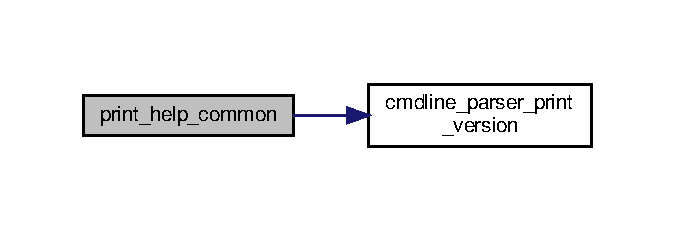
\includegraphics[width=324pt]{cmdline_8c_ad600bb9026825a295ea57df22bdf7eca_cgraph}
\end{center}
\end{figure}
\mbox{\Hypertarget{cmdline_8c_a21d8824d410efa489c4921011c1c0765}\label{cmdline_8c_a21d8824d410efa489c4921011c1c0765}} 
\index{cmdline.\+c@{cmdline.\+c}!update\+\_\+arg@{update\+\_\+arg}}
\index{update\+\_\+arg@{update\+\_\+arg}!cmdline.\+c@{cmdline.\+c}}
\subsubsection{\texorpdfstring{update\+\_\+arg()}{update\_arg()}}
{\footnotesize\ttfamily static int update\+\_\+arg (\begin{DoxyParamCaption}\item[{void $\ast$}]{field,  }\item[{char $\ast$$\ast$}]{orig\+\_\+field,  }\item[{unsigned int $\ast$}]{field\+\_\+given,  }\item[{unsigned int $\ast$}]{prev\+\_\+given,  }\item[{char $\ast$}]{value,  }\item[{char $\ast$}]{possible\+\_\+values\mbox{[}$\,$\mbox{]},  }\item[{\hyperlink{getopt_8c_a2c212835823e3c54a8ab6d95c652660e}{const} char $\ast$}]{default\+\_\+value,  }\item[{\hyperlink{cmdline_8c_a88e31a859f36efa57ad64e6ae13332a1}{cmdline\+\_\+parser\+\_\+arg\+\_\+type}}]{arg\+\_\+type,  }\item[{int}]{check\+\_\+ambiguity,  }\item[{int}]{override,  }\item[{int}]{no\+\_\+free,  }\item[{int}]{multiple\+\_\+option,  }\item[{\hyperlink{getopt_8c_a2c212835823e3c54a8ab6d95c652660e}{const} char $\ast$}]{long\+\_\+opt,  }\item[{char}]{short\+\_\+opt,  }\item[{\hyperlink{getopt_8c_a2c212835823e3c54a8ab6d95c652660e}{const} char $\ast$}]{additional\+\_\+error }\end{DoxyParamCaption})\hspace{0.3cm}{\ttfamily [static]}}



updates an option 


\begin{DoxyParams}{Parameters}
{\em field} & the generic pointer to the field to update \\
\hline
{\em orig\+\_\+field} & the pointer to the orig field \\
\hline
{\em field\+\_\+given} & the pointer to the number of occurrence of this option \\
\hline
{\em prev\+\_\+given} & the pointer to the number of occurrence already seen \\
\hline
{\em value} & the argument for this option (if null no arg was specified) \\
\hline
{\em possible\+\_\+values} & the possible values for this option (if specified) \\
\hline
{\em default\+\_\+value} & the default value (in case the option only accepts fixed values) \\
\hline
{\em arg\+\_\+type} & the type of this option \\
\hline
{\em check\+\_\+ambiguity} & \\
\hline
\end{DoxyParams}
\begin{DoxySeeAlso}{See also}
\hyperlink{structcmdline__parser__params_a6e4442704fc40b0b655f7cc602f13ec4}{cmdline\+\_\+parser\+\_\+params.\+check\+\_\+ambiguity} 
\end{DoxySeeAlso}

\begin{DoxyParams}{Parameters}
{\em override} & \\
\hline
\end{DoxyParams}
\begin{DoxySeeAlso}{See also}
\hyperlink{structcmdline__parser__params_ad3ff9d69146e69a47506782197b5675c}{cmdline\+\_\+parser\+\_\+params.\+override} 
\end{DoxySeeAlso}

\begin{DoxyParams}{Parameters}
{\em no\+\_\+free} & whether to free a possible previous value \\
\hline
{\em multiple\+\_\+option} & whether this is a multiple option \\
\hline
{\em long\+\_\+opt} & the corresponding long option \\
\hline
{\em short\+\_\+opt} & the corresponding short option (or \textquotesingle{}-\/\textquotesingle{} if none) \\
\hline
{\em additional\+\_\+error} & possible further error specification \\
\hline
\end{DoxyParams}
Here is the call graph for this function\+:
\nopagebreak
\begin{figure}[H]
\begin{center}
\leavevmode
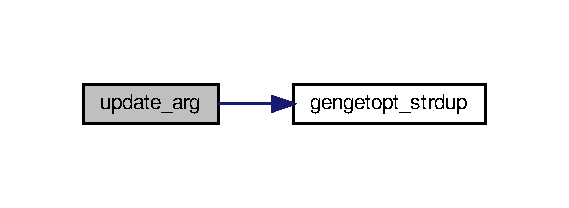
\includegraphics[width=273pt]{cmdline_8c_a21d8824d410efa489c4921011c1c0765_cgraph}
\end{center}
\end{figure}
\mbox{\Hypertarget{cmdline_8c_a332041b3060103618ef6b767ab32d0dd}\label{cmdline_8c_a332041b3060103618ef6b767ab32d0dd}} 
\index{cmdline.\+c@{cmdline.\+c}!write\+\_\+into\+\_\+file@{write\+\_\+into\+\_\+file}}
\index{write\+\_\+into\+\_\+file@{write\+\_\+into\+\_\+file}!cmdline.\+c@{cmdline.\+c}}
\subsubsection{\texorpdfstring{write\+\_\+into\+\_\+file()}{write\_into\_file()}}
{\footnotesize\ttfamily static void write\+\_\+into\+\_\+file (\begin{DoxyParamCaption}\item[{F\+I\+LE $\ast$}]{outfile,  }\item[{\hyperlink{getopt_8c_a2c212835823e3c54a8ab6d95c652660e}{const} char $\ast$}]{opt,  }\item[{\hyperlink{getopt_8c_a2c212835823e3c54a8ab6d95c652660e}{const} char $\ast$}]{arg,  }\item[{char $\ast$}]{values\mbox{[}$\,$\mbox{]} }\end{DoxyParamCaption})\hspace{0.3cm}{\ttfamily [static]}}



\subsection{Variable Documentation}
\mbox{\Hypertarget{cmdline_8c_accad6107ca685f6eba555f6ce63d355d}\label{cmdline_8c_accad6107ca685f6eba555f6ce63d355d}} 
\index{cmdline.\+c@{cmdline.\+c}!gengetopt\+\_\+args\+\_\+info\+\_\+description@{gengetopt\+\_\+args\+\_\+info\+\_\+description}}
\index{gengetopt\+\_\+args\+\_\+info\+\_\+description@{gengetopt\+\_\+args\+\_\+info\+\_\+description}!cmdline.\+c@{cmdline.\+c}}
\subsubsection{\texorpdfstring{gengetopt\+\_\+args\+\_\+info\+\_\+description}{gengetopt\_args\_info\_description}}
{\footnotesize\ttfamily \hyperlink{getopt_8c_a2c212835823e3c54a8ab6d95c652660e}{const} char$\ast$ gengetopt\+\_\+args\+\_\+info\+\_\+description = \char`\"{}\char`\"{}}

\mbox{\Hypertarget{cmdline_8c_a6af7a6b7fb37c0abaa916ee1cfa0a41f}\label{cmdline_8c_a6af7a6b7fb37c0abaa916ee1cfa0a41f}} 
\index{cmdline.\+c@{cmdline.\+c}!gengetopt\+\_\+args\+\_\+info\+\_\+help@{gengetopt\+\_\+args\+\_\+info\+\_\+help}}
\index{gengetopt\+\_\+args\+\_\+info\+\_\+help@{gengetopt\+\_\+args\+\_\+info\+\_\+help}!cmdline.\+c@{cmdline.\+c}}
\subsubsection{\texorpdfstring{gengetopt\+\_\+args\+\_\+info\+\_\+help}{gengetopt\_args\_info\_help}}
{\footnotesize\ttfamily \hyperlink{getopt_8c_a2c212835823e3c54a8ab6d95c652660e}{const} char$\ast$ gengetopt\+\_\+args\+\_\+info\+\_\+help\mbox{[}$\,$\mbox{]}}

{\bfseries Initial value\+:}
\begin{DoxyCode}
= \{
  \textcolor{stringliteral}{"  -h, --help               Print help and exit"},
  \textcolor{stringliteral}{"  -V, --version            Print version and exit"},
  \textcolor{stringliteral}{"  -o, --outfile=STRING     Output filename"},
  \textcolor{stringliteral}{"  -g, --gtf                GTF output  (default=off)"},
  \textcolor{stringliteral}{"  -t, --tabular            Tab delimited output  (default=off)"},
  \textcolor{stringliteral}{"  -b, --best-only          Print only best hit per alignment  (default=off)"},
  \textcolor{stringliteral}{"  -r, --best-region        Print all best non-overlapping hits per alignment  \(\backslash\)n                        
           (default=off)"},
  \textcolor{stringliteral}{"  -c, --pars=STRING        String with parameters"},
  \textcolor{stringliteral}{"  -s, --stop-early         Don't calculate p-values if below cutoff  \(\backslash\)n                            
       (default=off)"},
  \textcolor{stringliteral}{"  -n, --num-samples=INT    Number of samples"},
  \textcolor{stringliteral}{"  -p, --cutoff=FLOAT       p-value cutoff"},
  \textcolor{stringliteral}{"  -z, --debug-file=STRING  Debug file"},
  \textcolor{stringliteral}{"  -e, --eps                Postscript output  (default=off)"},
  \textcolor{stringliteral}{"  -i, --eps-cutoff=FLOAT   Postscript output p-value cutoff"},
  \textcolor{stringliteral}{"  -d, --eps-dir=STRING     Postscript directory"},
  \textcolor{stringliteral}{"  -l, --limit=STRING       limit to species"},
  \textcolor{stringliteral}{"  -m, --blosum=INT         BLOSUM matrix version"},
    0
\}
\end{DoxyCode}


all the lines making the help output 

\mbox{\Hypertarget{cmdline_8c_a610c3307abce5a8fd304b86b018ae60b}\label{cmdline_8c_a610c3307abce5a8fd304b86b018ae60b}} 
\index{cmdline.\+c@{cmdline.\+c}!gengetopt\+\_\+args\+\_\+info\+\_\+purpose@{gengetopt\+\_\+args\+\_\+info\+\_\+purpose}}
\index{gengetopt\+\_\+args\+\_\+info\+\_\+purpose@{gengetopt\+\_\+args\+\_\+info\+\_\+purpose}!cmdline.\+c@{cmdline.\+c}}
\subsubsection{\texorpdfstring{gengetopt\+\_\+args\+\_\+info\+\_\+purpose}{gengetopt\_args\_info\_purpose}}
{\footnotesize\ttfamily \hyperlink{getopt_8c_a2c212835823e3c54a8ab6d95c652660e}{const} char$\ast$ gengetopt\+\_\+args\+\_\+info\+\_\+purpose = \char`\"{}\char`\"{}}



the purpose string of the program 

\mbox{\Hypertarget{cmdline_8c_a9f397a306f363bfdebb611e86acf36d5}\label{cmdline_8c_a9f397a306f363bfdebb611e86acf36d5}} 
\index{cmdline.\+c@{cmdline.\+c}!gengetopt\+\_\+args\+\_\+info\+\_\+usage@{gengetopt\+\_\+args\+\_\+info\+\_\+usage}}
\index{gengetopt\+\_\+args\+\_\+info\+\_\+usage@{gengetopt\+\_\+args\+\_\+info\+\_\+usage}!cmdline.\+c@{cmdline.\+c}}
\subsubsection{\texorpdfstring{gengetopt\+\_\+args\+\_\+info\+\_\+usage}{gengetopt\_args\_info\_usage}}
{\footnotesize\ttfamily \hyperlink{getopt_8c_a2c212835823e3c54a8ab6d95c652660e}{const} char$\ast$ gengetopt\+\_\+args\+\_\+info\+\_\+usage = \char`\"{}Usage\+: \char`\"{} C\+M\+D\+L\+I\+N\+E\+\_\+\+P\+A\+R\+S\+E\+R\+\_\+\+P\+A\+C\+K\+A\+GE \char`\"{} \mbox{[}O\+P\+T\+I\+O\+NS\mbox{]}... \mbox{[}F\+I\+L\+ES\mbox{]}...\char`\"{}}



the usage string of the program 

\mbox{\Hypertarget{cmdline_8c_a08f16a026de44b77c5e7be490fb9e32b}\label{cmdline_8c_a08f16a026de44b77c5e7be490fb9e32b}} 
\index{cmdline.\+c@{cmdline.\+c}!package\+\_\+name@{package\+\_\+name}}
\index{package\+\_\+name@{package\+\_\+name}!cmdline.\+c@{cmdline.\+c}}
\subsubsection{\texorpdfstring{package\+\_\+name}{package\_name}}
{\footnotesize\ttfamily char$\ast$ package\+\_\+name = 0\hspace{0.3cm}{\ttfamily [static]}}


\hypertarget{cmdline_8h}{}\section{cmdline.\+h File Reference}
\label{cmdline_8h}\index{cmdline.\+h@{cmdline.\+h}}


The header file for the command line option parser generated by G\+NU Gengetopt version 2.\+22.\+1 \href{http://www.gnu.org/software/gengetopt}{\tt http\+://www.\+gnu.\+org/software/gengetopt}. DO N\+OT modify this file, since it can be overwritten.  


{\ttfamily \#include $<$stdio.\+h$>$}\newline
Include dependency graph for cmdline.\+h\+:
\nopagebreak
\begin{figure}[H]
\begin{center}
\leavevmode
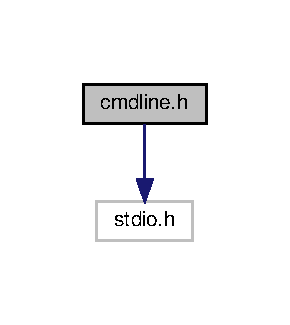
\includegraphics[width=139pt]{cmdline_8h__incl}
\end{center}
\end{figure}
This graph shows which files directly or indirectly include this file\+:
\nopagebreak
\begin{figure}[H]
\begin{center}
\leavevmode
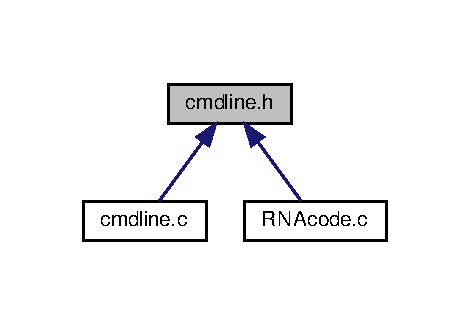
\includegraphics[width=226pt]{cmdline_8h__dep__incl}
\end{center}
\end{figure}
\subsection*{Classes}
\begin{DoxyCompactItemize}
\item 
struct \hyperlink{structgengetopt__args__info}{gengetopt\+\_\+args\+\_\+info}
\begin{DoxyCompactList}\small\item\em Where the command line options are stored. \end{DoxyCompactList}\item 
struct \hyperlink{structcmdline__parser__params}{cmdline\+\_\+parser\+\_\+params}
\begin{DoxyCompactList}\small\item\em The additional parameters to pass to parser functions. \end{DoxyCompactList}\end{DoxyCompactItemize}
\subsection*{Macros}
\begin{DoxyCompactItemize}
\item 
\#define \hyperlink{cmdline_8h_aeb847973552c32bcbe5f14973a0a8a32}{C\+M\+D\+L\+I\+N\+E\+\_\+\+P\+A\+R\+S\+E\+R\+\_\+\+P\+A\+C\+K\+A\+GE}~P\+A\+C\+K\+A\+GE
\begin{DoxyCompactList}\small\item\em the program name \end{DoxyCompactList}\item 
\#define \hyperlink{cmdline_8h_a1eeca7dc254bf6867ba9635f45771471}{C\+M\+D\+L\+I\+N\+E\+\_\+\+P\+A\+R\+S\+E\+R\+\_\+\+V\+E\+R\+S\+I\+ON}~V\+E\+R\+S\+I\+ON
\begin{DoxyCompactList}\small\item\em the program version \end{DoxyCompactList}\end{DoxyCompactItemize}
\subsection*{Functions}
\begin{DoxyCompactItemize}
\item 
int \hyperlink{cmdline_8h_a96f1044799c552f3ee139f9b1387b363}{cmdline\+\_\+parser} (int argc, char $\ast$\hyperlink{getopt_8c_a2c212835823e3c54a8ab6d95c652660e}{const} $\ast$argv, struct \hyperlink{structgengetopt__args__info}{gengetopt\+\_\+args\+\_\+info} $\ast$args\+\_\+info)
\item 
int \hyperlink{cmdline_8h_a08e3536edc64ec5ee7c2df546c6e9dd7}{cmdline\+\_\+parser2} (int argc, char $\ast$\hyperlink{getopt_8c_a2c212835823e3c54a8ab6d95c652660e}{const} $\ast$argv, struct \hyperlink{structgengetopt__args__info}{gengetopt\+\_\+args\+\_\+info} $\ast$args\+\_\+info, int override, int initialize, int check\+\_\+required)
\item 
int \hyperlink{cmdline_8h_a77e461b5bdfd4a36c59a96bfb1813e38}{cmdline\+\_\+parser\+\_\+ext} (int argc, char $\ast$\hyperlink{getopt_8c_a2c212835823e3c54a8ab6d95c652660e}{const} $\ast$argv, struct \hyperlink{structgengetopt__args__info}{gengetopt\+\_\+args\+\_\+info} $\ast$args\+\_\+info, struct \hyperlink{structcmdline__parser__params}{cmdline\+\_\+parser\+\_\+params} $\ast$params)
\item 
int \hyperlink{cmdline_8h_a1f73418092a6e6eb3706aa0de2785e11}{cmdline\+\_\+parser\+\_\+dump} (F\+I\+LE $\ast$\hyperlink{postscript_8c_ae581849c67336453bd5b81e6518019a9}{outfile}, struct \hyperlink{structgengetopt__args__info}{gengetopt\+\_\+args\+\_\+info} $\ast$args\+\_\+info)
\item 
int \hyperlink{cmdline_8h_a5f3e9412f88f1058a31ac28ad2ea2818}{cmdline\+\_\+parser\+\_\+file\+\_\+save} (\hyperlink{getopt_8c_a2c212835823e3c54a8ab6d95c652660e}{const} char $\ast$filename, struct \hyperlink{structgengetopt__args__info}{gengetopt\+\_\+args\+\_\+info} $\ast$args\+\_\+info)
\item 
void \hyperlink{cmdline_8h_ad4f7db2fa4002379eb30e5206f3b7492}{cmdline\+\_\+parser\+\_\+print\+\_\+help} (void)
\item 
void \hyperlink{cmdline_8h_a96f27bf35ce0ab8eea7a1f6e6b59a5e2}{cmdline\+\_\+parser\+\_\+print\+\_\+version} (void)
\item 
void \hyperlink{cmdline_8h_af72b814611cffc706b2135ccdfe7e997}{cmdline\+\_\+parser\+\_\+params\+\_\+init} (struct \hyperlink{structcmdline__parser__params}{cmdline\+\_\+parser\+\_\+params} $\ast$params)
\item 
struct \hyperlink{structcmdline__parser__params}{cmdline\+\_\+parser\+\_\+params} $\ast$ \hyperlink{cmdline_8h_afd778af110fe0ee1ea5eac7aa9939d92}{cmdline\+\_\+parser\+\_\+params\+\_\+create} (void)
\item 
void \hyperlink{cmdline_8h_aca62b50d03d0d082968eeb1940f98650}{cmdline\+\_\+parser\+\_\+init} (struct \hyperlink{structgengetopt__args__info}{gengetopt\+\_\+args\+\_\+info} $\ast$args\+\_\+info)
\item 
void \hyperlink{cmdline_8h_af1b97c4e92b88f736e350b3902266ba4}{cmdline\+\_\+parser\+\_\+free} (struct \hyperlink{structgengetopt__args__info}{gengetopt\+\_\+args\+\_\+info} $\ast$args\+\_\+info)
\item 
int \hyperlink{cmdline_8h_a83651e5be280d60aed58fdb72456a030}{cmdline\+\_\+parser\+\_\+required} (struct \hyperlink{structgengetopt__args__info}{gengetopt\+\_\+args\+\_\+info} $\ast$args\+\_\+info, \hyperlink{getopt_8c_a2c212835823e3c54a8ab6d95c652660e}{const} char $\ast$prog\+\_\+name)
\end{DoxyCompactItemize}
\subsection*{Variables}
\begin{DoxyCompactItemize}
\item 
\hyperlink{getopt_8c_a2c212835823e3c54a8ab6d95c652660e}{const} char $\ast$ \hyperlink{cmdline_8h_a610c3307abce5a8fd304b86b018ae60b}{gengetopt\+\_\+args\+\_\+info\+\_\+purpose}
\begin{DoxyCompactList}\small\item\em the purpose string of the program \end{DoxyCompactList}\item 
\hyperlink{getopt_8c_a2c212835823e3c54a8ab6d95c652660e}{const} char $\ast$ \hyperlink{cmdline_8h_a9f397a306f363bfdebb611e86acf36d5}{gengetopt\+\_\+args\+\_\+info\+\_\+usage}
\begin{DoxyCompactList}\small\item\em the usage string of the program \end{DoxyCompactList}\item 
\hyperlink{getopt_8c_a2c212835823e3c54a8ab6d95c652660e}{const} char $\ast$ \hyperlink{cmdline_8h_a6af7a6b7fb37c0abaa916ee1cfa0a41f}{gengetopt\+\_\+args\+\_\+info\+\_\+help} \mbox{[}$\,$\mbox{]}
\begin{DoxyCompactList}\small\item\em all the lines making the help output \end{DoxyCompactList}\end{DoxyCompactItemize}


\subsection{Detailed Description}
The header file for the command line option parser generated by G\+NU Gengetopt version 2.\+22.\+1 \href{http://www.gnu.org/software/gengetopt}{\tt http\+://www.\+gnu.\+org/software/gengetopt}. DO N\+OT modify this file, since it can be overwritten. 

\begin{DoxyAuthor}{Author}
G\+NU Gengetopt by Lorenzo Bettini 
\end{DoxyAuthor}


\subsection{Macro Definition Documentation}
\mbox{\Hypertarget{cmdline_8h_aeb847973552c32bcbe5f14973a0a8a32}\label{cmdline_8h_aeb847973552c32bcbe5f14973a0a8a32}} 
\index{cmdline.\+h@{cmdline.\+h}!C\+M\+D\+L\+I\+N\+E\+\_\+\+P\+A\+R\+S\+E\+R\+\_\+\+P\+A\+C\+K\+A\+GE@{C\+M\+D\+L\+I\+N\+E\+\_\+\+P\+A\+R\+S\+E\+R\+\_\+\+P\+A\+C\+K\+A\+GE}}
\index{C\+M\+D\+L\+I\+N\+E\+\_\+\+P\+A\+R\+S\+E\+R\+\_\+\+P\+A\+C\+K\+A\+GE@{C\+M\+D\+L\+I\+N\+E\+\_\+\+P\+A\+R\+S\+E\+R\+\_\+\+P\+A\+C\+K\+A\+GE}!cmdline.\+h@{cmdline.\+h}}
\subsubsection{\texorpdfstring{C\+M\+D\+L\+I\+N\+E\+\_\+\+P\+A\+R\+S\+E\+R\+\_\+\+P\+A\+C\+K\+A\+GE}{CMDLINE\_PARSER\_PACKAGE}}
{\footnotesize\ttfamily \#define C\+M\+D\+L\+I\+N\+E\+\_\+\+P\+A\+R\+S\+E\+R\+\_\+\+P\+A\+C\+K\+A\+GE~P\+A\+C\+K\+A\+GE}



the program name 

\mbox{\Hypertarget{cmdline_8h_a1eeca7dc254bf6867ba9635f45771471}\label{cmdline_8h_a1eeca7dc254bf6867ba9635f45771471}} 
\index{cmdline.\+h@{cmdline.\+h}!C\+M\+D\+L\+I\+N\+E\+\_\+\+P\+A\+R\+S\+E\+R\+\_\+\+V\+E\+R\+S\+I\+ON@{C\+M\+D\+L\+I\+N\+E\+\_\+\+P\+A\+R\+S\+E\+R\+\_\+\+V\+E\+R\+S\+I\+ON}}
\index{C\+M\+D\+L\+I\+N\+E\+\_\+\+P\+A\+R\+S\+E\+R\+\_\+\+V\+E\+R\+S\+I\+ON@{C\+M\+D\+L\+I\+N\+E\+\_\+\+P\+A\+R\+S\+E\+R\+\_\+\+V\+E\+R\+S\+I\+ON}!cmdline.\+h@{cmdline.\+h}}
\subsubsection{\texorpdfstring{C\+M\+D\+L\+I\+N\+E\+\_\+\+P\+A\+R\+S\+E\+R\+\_\+\+V\+E\+R\+S\+I\+ON}{CMDLINE\_PARSER\_VERSION}}
{\footnotesize\ttfamily \#define C\+M\+D\+L\+I\+N\+E\+\_\+\+P\+A\+R\+S\+E\+R\+\_\+\+V\+E\+R\+S\+I\+ON~V\+E\+R\+S\+I\+ON}



the program version 



\subsection{Function Documentation}
\mbox{\Hypertarget{cmdline_8h_a96f1044799c552f3ee139f9b1387b363}\label{cmdline_8h_a96f1044799c552f3ee139f9b1387b363}} 
\index{cmdline.\+h@{cmdline.\+h}!cmdline\+\_\+parser@{cmdline\+\_\+parser}}
\index{cmdline\+\_\+parser@{cmdline\+\_\+parser}!cmdline.\+h@{cmdline.\+h}}
\subsubsection{\texorpdfstring{cmdline\+\_\+parser()}{cmdline\_parser()}}
{\footnotesize\ttfamily int cmdline\+\_\+parser (\begin{DoxyParamCaption}\item[{int}]{argc,  }\item[{char $\ast$\hyperlink{getopt_8c_a2c212835823e3c54a8ab6d95c652660e}{const} $\ast$}]{argv,  }\item[{struct \hyperlink{structgengetopt__args__info}{gengetopt\+\_\+args\+\_\+info} $\ast$}]{args\+\_\+info }\end{DoxyParamCaption})}

The command line parser 
\begin{DoxyParams}{Parameters}
{\em argc} & the number of command line options \\
\hline
{\em argv} & the command line options \\
\hline
{\em args\+\_\+info} & the structure where option information will be stored \\
\hline
\end{DoxyParams}
\begin{DoxyReturn}{Returns}
0 if everything went fine, N\+ON 0 if an error took place 
\end{DoxyReturn}
Here is the call graph for this function\+:
\nopagebreak
\begin{figure}[H]
\begin{center}
\leavevmode
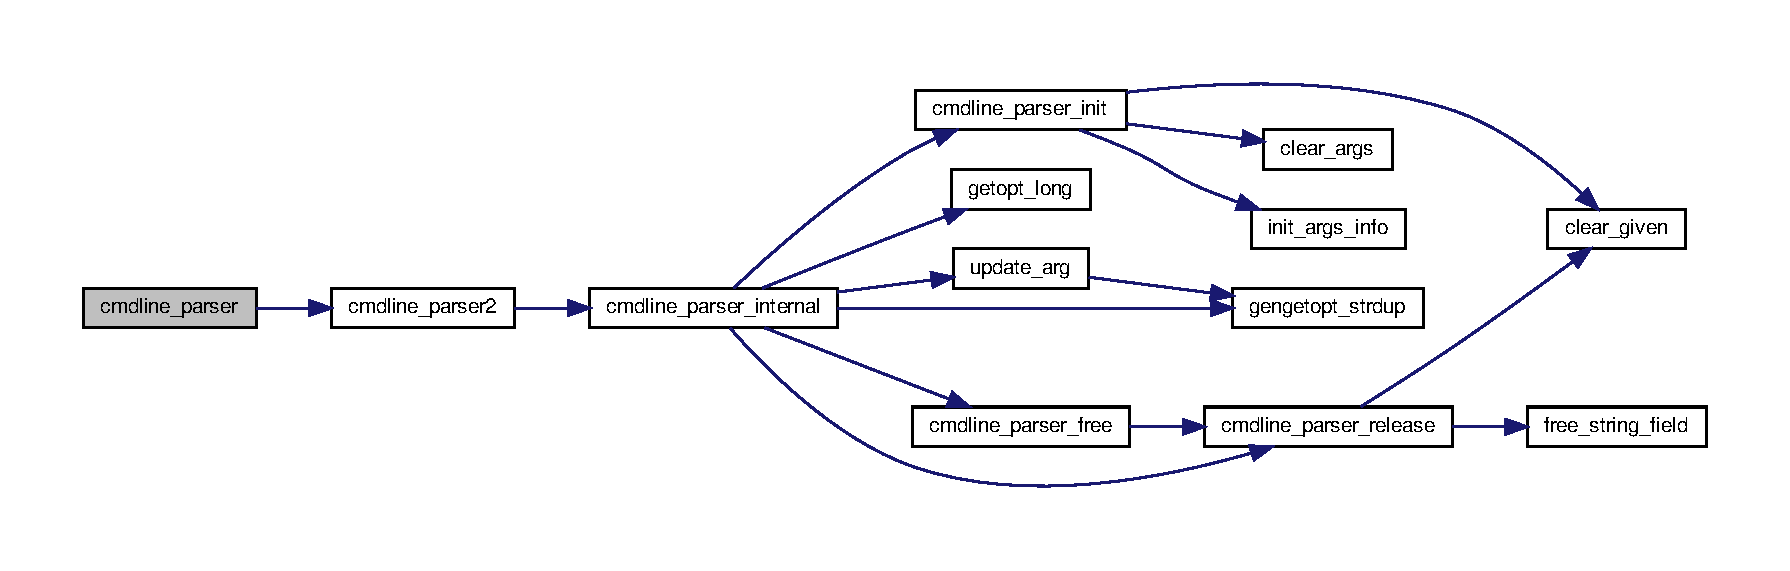
\includegraphics[width=350pt]{cmdline_8h_a96f1044799c552f3ee139f9b1387b363_cgraph}
\end{center}
\end{figure}
\mbox{\Hypertarget{cmdline_8h_a08e3536edc64ec5ee7c2df546c6e9dd7}\label{cmdline_8h_a08e3536edc64ec5ee7c2df546c6e9dd7}} 
\index{cmdline.\+h@{cmdline.\+h}!cmdline\+\_\+parser2@{cmdline\+\_\+parser2}}
\index{cmdline\+\_\+parser2@{cmdline\+\_\+parser2}!cmdline.\+h@{cmdline.\+h}}
\subsubsection{\texorpdfstring{cmdline\+\_\+parser2()}{cmdline\_parser2()}}
{\footnotesize\ttfamily int cmdline\+\_\+parser2 (\begin{DoxyParamCaption}\item[{int}]{argc,  }\item[{char $\ast$\hyperlink{getopt_8c_a2c212835823e3c54a8ab6d95c652660e}{const} $\ast$}]{argv,  }\item[{struct \hyperlink{structgengetopt__args__info}{gengetopt\+\_\+args\+\_\+info} $\ast$}]{args\+\_\+info,  }\item[{int}]{override,  }\item[{int}]{initialize,  }\item[{int}]{check\+\_\+required }\end{DoxyParamCaption})}

The command line parser (version with additional parameters -\/ deprecated) 
\begin{DoxyParams}{Parameters}
{\em argc} & the number of command line options \\
\hline
{\em argv} & the command line options \\
\hline
{\em args\+\_\+info} & the structure where option information will be stored \\
\hline
{\em override} & whether to override possibly already present options \\
\hline
{\em initialize} & whether to initialize the option structure my\+\_\+args\+\_\+info \\
\hline
{\em check\+\_\+required} & whether to check that all required options were provided \\
\hline
\end{DoxyParams}
\begin{DoxyReturn}{Returns}
0 if everything went fine, N\+ON 0 if an error took place 
\end{DoxyReturn}
\begin{DoxyRefDesc}{Deprecated}
\item[\hyperlink{deprecated__deprecated000001}{Deprecated}]use \hyperlink{cmdline_8h_a77e461b5bdfd4a36c59a96bfb1813e38}{cmdline\+\_\+parser\+\_\+ext()} instead \end{DoxyRefDesc}
Here is the call graph for this function\+:
\nopagebreak
\begin{figure}[H]
\begin{center}
\leavevmode
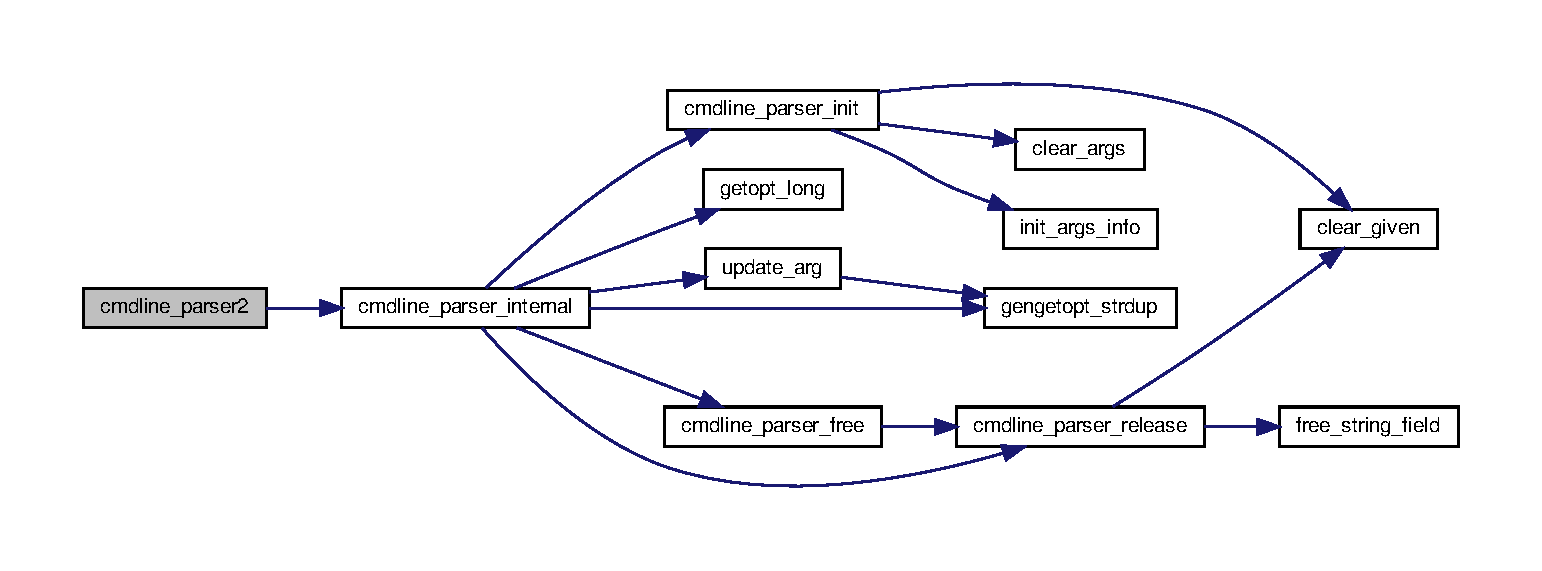
\includegraphics[width=350pt]{cmdline_8h_a08e3536edc64ec5ee7c2df546c6e9dd7_cgraph}
\end{center}
\end{figure}
\mbox{\Hypertarget{cmdline_8h_a1f73418092a6e6eb3706aa0de2785e11}\label{cmdline_8h_a1f73418092a6e6eb3706aa0de2785e11}} 
\index{cmdline.\+h@{cmdline.\+h}!cmdline\+\_\+parser\+\_\+dump@{cmdline\+\_\+parser\+\_\+dump}}
\index{cmdline\+\_\+parser\+\_\+dump@{cmdline\+\_\+parser\+\_\+dump}!cmdline.\+h@{cmdline.\+h}}
\subsubsection{\texorpdfstring{cmdline\+\_\+parser\+\_\+dump()}{cmdline\_parser\_dump()}}
{\footnotesize\ttfamily int cmdline\+\_\+parser\+\_\+dump (\begin{DoxyParamCaption}\item[{F\+I\+LE $\ast$}]{outfile,  }\item[{struct \hyperlink{structgengetopt__args__info}{gengetopt\+\_\+args\+\_\+info} $\ast$}]{args\+\_\+info }\end{DoxyParamCaption})}

Save the contents of the option struct into an already open F\+I\+LE stream. 
\begin{DoxyParams}{Parameters}
{\em outfile} & the stream where to dump options \\
\hline
{\em args\+\_\+info} & the option struct to dump \\
\hline
\end{DoxyParams}
\begin{DoxyReturn}{Returns}
0 if everything went fine, N\+ON 0 if an error took place 
\end{DoxyReturn}
Here is the call graph for this function\+:
\nopagebreak
\begin{figure}[H]
\begin{center}
\leavevmode
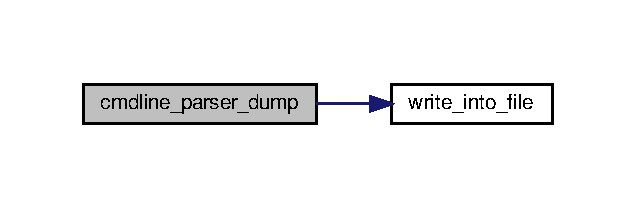
\includegraphics[width=305pt]{cmdline_8h_a1f73418092a6e6eb3706aa0de2785e11_cgraph}
\end{center}
\end{figure}
\mbox{\Hypertarget{cmdline_8h_a77e461b5bdfd4a36c59a96bfb1813e38}\label{cmdline_8h_a77e461b5bdfd4a36c59a96bfb1813e38}} 
\index{cmdline.\+h@{cmdline.\+h}!cmdline\+\_\+parser\+\_\+ext@{cmdline\+\_\+parser\+\_\+ext}}
\index{cmdline\+\_\+parser\+\_\+ext@{cmdline\+\_\+parser\+\_\+ext}!cmdline.\+h@{cmdline.\+h}}
\subsubsection{\texorpdfstring{cmdline\+\_\+parser\+\_\+ext()}{cmdline\_parser\_ext()}}
{\footnotesize\ttfamily int cmdline\+\_\+parser\+\_\+ext (\begin{DoxyParamCaption}\item[{int}]{argc,  }\item[{char $\ast$\hyperlink{getopt_8c_a2c212835823e3c54a8ab6d95c652660e}{const} $\ast$}]{argv,  }\item[{struct \hyperlink{structgengetopt__args__info}{gengetopt\+\_\+args\+\_\+info} $\ast$}]{args\+\_\+info,  }\item[{struct \hyperlink{structcmdline__parser__params}{cmdline\+\_\+parser\+\_\+params} $\ast$}]{params }\end{DoxyParamCaption})}

The command line parser (version with additional parameters) 
\begin{DoxyParams}{Parameters}
{\em argc} & the number of command line options \\
\hline
{\em argv} & the command line options \\
\hline
{\em args\+\_\+info} & the structure where option information will be stored \\
\hline
{\em params} & additional parameters for the parser \\
\hline
\end{DoxyParams}
\begin{DoxyReturn}{Returns}
0 if everything went fine, N\+ON 0 if an error took place 
\end{DoxyReturn}
Here is the call graph for this function\+:
\nopagebreak
\begin{figure}[H]
\begin{center}
\leavevmode
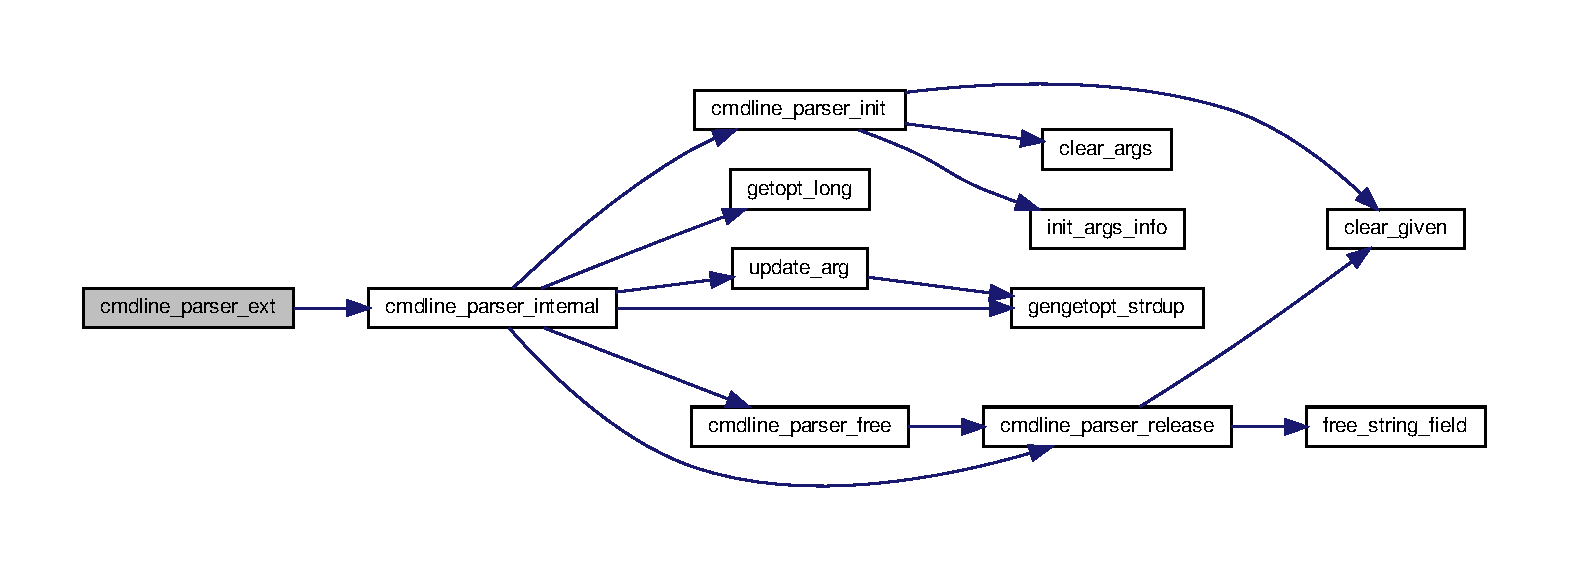
\includegraphics[width=350pt]{cmdline_8h_a77e461b5bdfd4a36c59a96bfb1813e38_cgraph}
\end{center}
\end{figure}
\mbox{\Hypertarget{cmdline_8h_a5f3e9412f88f1058a31ac28ad2ea2818}\label{cmdline_8h_a5f3e9412f88f1058a31ac28ad2ea2818}} 
\index{cmdline.\+h@{cmdline.\+h}!cmdline\+\_\+parser\+\_\+file\+\_\+save@{cmdline\+\_\+parser\+\_\+file\+\_\+save}}
\index{cmdline\+\_\+parser\+\_\+file\+\_\+save@{cmdline\+\_\+parser\+\_\+file\+\_\+save}!cmdline.\+h@{cmdline.\+h}}
\subsubsection{\texorpdfstring{cmdline\+\_\+parser\+\_\+file\+\_\+save()}{cmdline\_parser\_file\_save()}}
{\footnotesize\ttfamily int cmdline\+\_\+parser\+\_\+file\+\_\+save (\begin{DoxyParamCaption}\item[{\hyperlink{getopt_8c_a2c212835823e3c54a8ab6d95c652660e}{const} char $\ast$}]{filename,  }\item[{struct \hyperlink{structgengetopt__args__info}{gengetopt\+\_\+args\+\_\+info} $\ast$}]{args\+\_\+info }\end{DoxyParamCaption})}

Save the contents of the option struct into a (text) file. This file can be read by the config file parser (if generated by gengetopt) 
\begin{DoxyParams}{Parameters}
{\em filename} & the file where to save \\
\hline
{\em args\+\_\+info} & the option struct to save \\
\hline
\end{DoxyParams}
\begin{DoxyReturn}{Returns}
0 if everything went fine, N\+ON 0 if an error took place 
\end{DoxyReturn}
Here is the call graph for this function\+:
\nopagebreak
\begin{figure}[H]
\begin{center}
\leavevmode
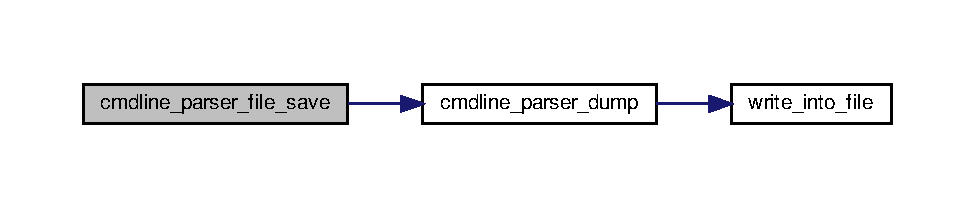
\includegraphics[width=350pt]{cmdline_8h_a5f3e9412f88f1058a31ac28ad2ea2818_cgraph}
\end{center}
\end{figure}
\mbox{\Hypertarget{cmdline_8h_af1b97c4e92b88f736e350b3902266ba4}\label{cmdline_8h_af1b97c4e92b88f736e350b3902266ba4}} 
\index{cmdline.\+h@{cmdline.\+h}!cmdline\+\_\+parser\+\_\+free@{cmdline\+\_\+parser\+\_\+free}}
\index{cmdline\+\_\+parser\+\_\+free@{cmdline\+\_\+parser\+\_\+free}!cmdline.\+h@{cmdline.\+h}}
\subsubsection{\texorpdfstring{cmdline\+\_\+parser\+\_\+free()}{cmdline\_parser\_free()}}
{\footnotesize\ttfamily void cmdline\+\_\+parser\+\_\+free (\begin{DoxyParamCaption}\item[{struct \hyperlink{structgengetopt__args__info}{gengetopt\+\_\+args\+\_\+info} $\ast$}]{args\+\_\+info }\end{DoxyParamCaption})}

Deallocates the string fields of the \hyperlink{structgengetopt__args__info}{gengetopt\+\_\+args\+\_\+info} structure (but does not deallocate the structure itself) 
\begin{DoxyParams}{Parameters}
{\em args\+\_\+info} & the structure to deallocate \\
\hline
\end{DoxyParams}
Here is the call graph for this function\+:
\nopagebreak
\begin{figure}[H]
\begin{center}
\leavevmode
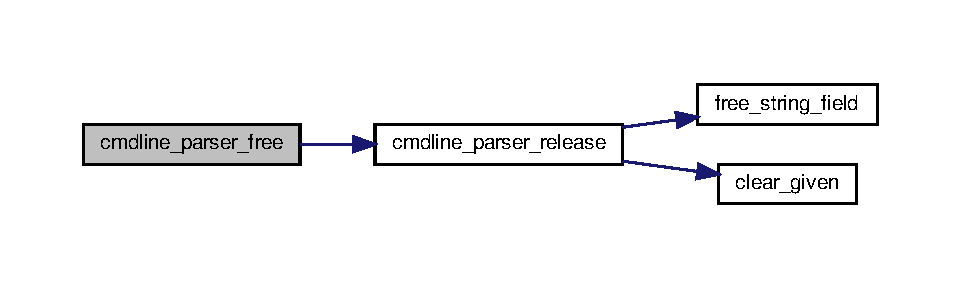
\includegraphics[width=350pt]{cmdline_8h_af1b97c4e92b88f736e350b3902266ba4_cgraph}
\end{center}
\end{figure}
\mbox{\Hypertarget{cmdline_8h_aca62b50d03d0d082968eeb1940f98650}\label{cmdline_8h_aca62b50d03d0d082968eeb1940f98650}} 
\index{cmdline.\+h@{cmdline.\+h}!cmdline\+\_\+parser\+\_\+init@{cmdline\+\_\+parser\+\_\+init}}
\index{cmdline\+\_\+parser\+\_\+init@{cmdline\+\_\+parser\+\_\+init}!cmdline.\+h@{cmdline.\+h}}
\subsubsection{\texorpdfstring{cmdline\+\_\+parser\+\_\+init()}{cmdline\_parser\_init()}}
{\footnotesize\ttfamily void cmdline\+\_\+parser\+\_\+init (\begin{DoxyParamCaption}\item[{struct \hyperlink{structgengetopt__args__info}{gengetopt\+\_\+args\+\_\+info} $\ast$}]{args\+\_\+info }\end{DoxyParamCaption})}

Initializes the passed \hyperlink{structgengetopt__args__info}{gengetopt\+\_\+args\+\_\+info} structure\textquotesingle{}s fields (also set default values for options that have a default) 
\begin{DoxyParams}{Parameters}
{\em args\+\_\+info} & the structure to initialize \\
\hline
\end{DoxyParams}
Here is the call graph for this function\+:
\nopagebreak
\begin{figure}[H]
\begin{center}
\leavevmode
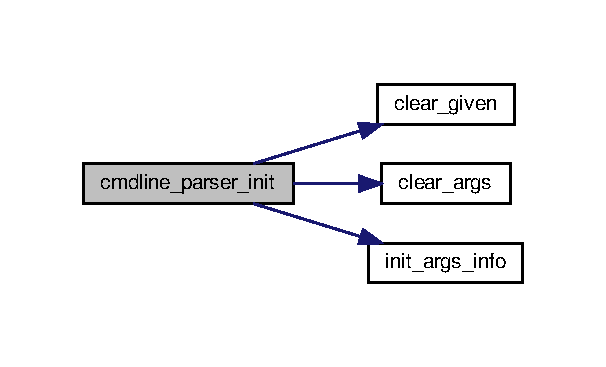
\includegraphics[width=291pt]{cmdline_8h_aca62b50d03d0d082968eeb1940f98650_cgraph}
\end{center}
\end{figure}
\mbox{\Hypertarget{cmdline_8h_afd778af110fe0ee1ea5eac7aa9939d92}\label{cmdline_8h_afd778af110fe0ee1ea5eac7aa9939d92}} 
\index{cmdline.\+h@{cmdline.\+h}!cmdline\+\_\+parser\+\_\+params\+\_\+create@{cmdline\+\_\+parser\+\_\+params\+\_\+create}}
\index{cmdline\+\_\+parser\+\_\+params\+\_\+create@{cmdline\+\_\+parser\+\_\+params\+\_\+create}!cmdline.\+h@{cmdline.\+h}}
\subsubsection{\texorpdfstring{cmdline\+\_\+parser\+\_\+params\+\_\+create()}{cmdline\_parser\_params\_create()}}
{\footnotesize\ttfamily struct \hyperlink{structcmdline__parser__params}{cmdline\+\_\+parser\+\_\+params}$\ast$ cmdline\+\_\+parser\+\_\+params\+\_\+create (\begin{DoxyParamCaption}\item[{void}]{ }\end{DoxyParamCaption})}

Allocates dynamically a \hyperlink{structcmdline__parser__params}{cmdline\+\_\+parser\+\_\+params} structure and initializes all its fields to their default values \begin{DoxyReturn}{Returns}
the created and initialized \hyperlink{structcmdline__parser__params}{cmdline\+\_\+parser\+\_\+params} structure 
\end{DoxyReturn}
Here is the call graph for this function\+:
\nopagebreak
\begin{figure}[H]
\begin{center}
\leavevmode
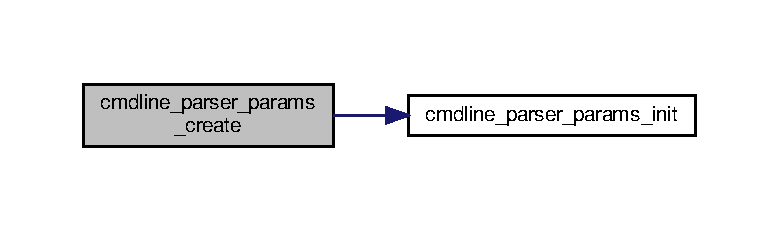
\includegraphics[width=350pt]{cmdline_8h_afd778af110fe0ee1ea5eac7aa9939d92_cgraph}
\end{center}
\end{figure}
\mbox{\Hypertarget{cmdline_8h_af72b814611cffc706b2135ccdfe7e997}\label{cmdline_8h_af72b814611cffc706b2135ccdfe7e997}} 
\index{cmdline.\+h@{cmdline.\+h}!cmdline\+\_\+parser\+\_\+params\+\_\+init@{cmdline\+\_\+parser\+\_\+params\+\_\+init}}
\index{cmdline\+\_\+parser\+\_\+params\+\_\+init@{cmdline\+\_\+parser\+\_\+params\+\_\+init}!cmdline.\+h@{cmdline.\+h}}
\subsubsection{\texorpdfstring{cmdline\+\_\+parser\+\_\+params\+\_\+init()}{cmdline\_parser\_params\_init()}}
{\footnotesize\ttfamily void cmdline\+\_\+parser\+\_\+params\+\_\+init (\begin{DoxyParamCaption}\item[{struct \hyperlink{structcmdline__parser__params}{cmdline\+\_\+parser\+\_\+params} $\ast$}]{params }\end{DoxyParamCaption})}

Initializes all the fields a \hyperlink{structcmdline__parser__params}{cmdline\+\_\+parser\+\_\+params} structure to their default values 
\begin{DoxyParams}{Parameters}
{\em params} & the structure to initialize \\
\hline
\end{DoxyParams}
\mbox{\Hypertarget{cmdline_8h_ad4f7db2fa4002379eb30e5206f3b7492}\label{cmdline_8h_ad4f7db2fa4002379eb30e5206f3b7492}} 
\index{cmdline.\+h@{cmdline.\+h}!cmdline\+\_\+parser\+\_\+print\+\_\+help@{cmdline\+\_\+parser\+\_\+print\+\_\+help}}
\index{cmdline\+\_\+parser\+\_\+print\+\_\+help@{cmdline\+\_\+parser\+\_\+print\+\_\+help}!cmdline.\+h@{cmdline.\+h}}
\subsubsection{\texorpdfstring{cmdline\+\_\+parser\+\_\+print\+\_\+help()}{cmdline\_parser\_print\_help()}}
{\footnotesize\ttfamily void cmdline\+\_\+parser\+\_\+print\+\_\+help (\begin{DoxyParamCaption}\item[{void}]{ }\end{DoxyParamCaption})}

Print the help Here is the call graph for this function\+:
\nopagebreak
\begin{figure}[H]
\begin{center}
\leavevmode
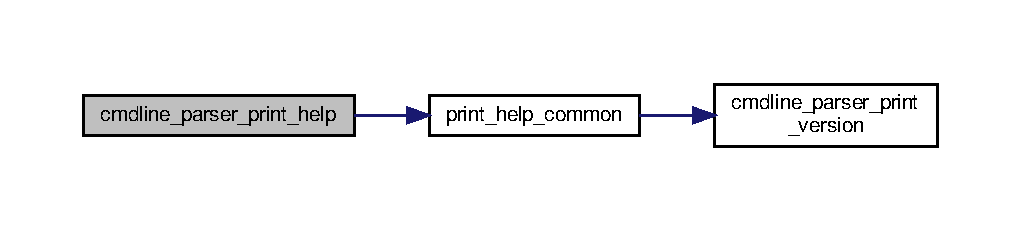
\includegraphics[width=350pt]{cmdline_8h_ad4f7db2fa4002379eb30e5206f3b7492_cgraph}
\end{center}
\end{figure}
\mbox{\Hypertarget{cmdline_8h_a96f27bf35ce0ab8eea7a1f6e6b59a5e2}\label{cmdline_8h_a96f27bf35ce0ab8eea7a1f6e6b59a5e2}} 
\index{cmdline.\+h@{cmdline.\+h}!cmdline\+\_\+parser\+\_\+print\+\_\+version@{cmdline\+\_\+parser\+\_\+print\+\_\+version}}
\index{cmdline\+\_\+parser\+\_\+print\+\_\+version@{cmdline\+\_\+parser\+\_\+print\+\_\+version}!cmdline.\+h@{cmdline.\+h}}
\subsubsection{\texorpdfstring{cmdline\+\_\+parser\+\_\+print\+\_\+version()}{cmdline\_parser\_print\_version()}}
{\footnotesize\ttfamily void cmdline\+\_\+parser\+\_\+print\+\_\+version (\begin{DoxyParamCaption}\item[{void}]{ }\end{DoxyParamCaption})}

Print the version \mbox{\Hypertarget{cmdline_8h_a83651e5be280d60aed58fdb72456a030}\label{cmdline_8h_a83651e5be280d60aed58fdb72456a030}} 
\index{cmdline.\+h@{cmdline.\+h}!cmdline\+\_\+parser\+\_\+required@{cmdline\+\_\+parser\+\_\+required}}
\index{cmdline\+\_\+parser\+\_\+required@{cmdline\+\_\+parser\+\_\+required}!cmdline.\+h@{cmdline.\+h}}
\subsubsection{\texorpdfstring{cmdline\+\_\+parser\+\_\+required()}{cmdline\_parser\_required()}}
{\footnotesize\ttfamily int cmdline\+\_\+parser\+\_\+required (\begin{DoxyParamCaption}\item[{struct \hyperlink{structgengetopt__args__info}{gengetopt\+\_\+args\+\_\+info} $\ast$}]{args\+\_\+info,  }\item[{\hyperlink{getopt_8c_a2c212835823e3c54a8ab6d95c652660e}{const} char $\ast$}]{prog\+\_\+name }\end{DoxyParamCaption})}

Checks that all the required options were specified 
\begin{DoxyParams}{Parameters}
{\em args\+\_\+info} & the structure to check \\
\hline
{\em prog\+\_\+name} & the name of the program that will be used to print possible errors \\
\hline
\end{DoxyParams}
\begin{DoxyReturn}{Returns}

\end{DoxyReturn}


\subsection{Variable Documentation}
\mbox{\Hypertarget{cmdline_8h_a6af7a6b7fb37c0abaa916ee1cfa0a41f}\label{cmdline_8h_a6af7a6b7fb37c0abaa916ee1cfa0a41f}} 
\index{cmdline.\+h@{cmdline.\+h}!gengetopt\+\_\+args\+\_\+info\+\_\+help@{gengetopt\+\_\+args\+\_\+info\+\_\+help}}
\index{gengetopt\+\_\+args\+\_\+info\+\_\+help@{gengetopt\+\_\+args\+\_\+info\+\_\+help}!cmdline.\+h@{cmdline.\+h}}
\subsubsection{\texorpdfstring{gengetopt\+\_\+args\+\_\+info\+\_\+help}{gengetopt\_args\_info\_help}}
{\footnotesize\ttfamily \hyperlink{getopt_8c_a2c212835823e3c54a8ab6d95c652660e}{const} char$\ast$ gengetopt\+\_\+args\+\_\+info\+\_\+help\mbox{[}$\,$\mbox{]}}



all the lines making the help output 

\mbox{\Hypertarget{cmdline_8h_a610c3307abce5a8fd304b86b018ae60b}\label{cmdline_8h_a610c3307abce5a8fd304b86b018ae60b}} 
\index{cmdline.\+h@{cmdline.\+h}!gengetopt\+\_\+args\+\_\+info\+\_\+purpose@{gengetopt\+\_\+args\+\_\+info\+\_\+purpose}}
\index{gengetopt\+\_\+args\+\_\+info\+\_\+purpose@{gengetopt\+\_\+args\+\_\+info\+\_\+purpose}!cmdline.\+h@{cmdline.\+h}}
\subsubsection{\texorpdfstring{gengetopt\+\_\+args\+\_\+info\+\_\+purpose}{gengetopt\_args\_info\_purpose}}
{\footnotesize\ttfamily \hyperlink{getopt_8c_a2c212835823e3c54a8ab6d95c652660e}{const} char$\ast$ gengetopt\+\_\+args\+\_\+info\+\_\+purpose}



the purpose string of the program 

\mbox{\Hypertarget{cmdline_8h_a9f397a306f363bfdebb611e86acf36d5}\label{cmdline_8h_a9f397a306f363bfdebb611e86acf36d5}} 
\index{cmdline.\+h@{cmdline.\+h}!gengetopt\+\_\+args\+\_\+info\+\_\+usage@{gengetopt\+\_\+args\+\_\+info\+\_\+usage}}
\index{gengetopt\+\_\+args\+\_\+info\+\_\+usage@{gengetopt\+\_\+args\+\_\+info\+\_\+usage}!cmdline.\+h@{cmdline.\+h}}
\subsubsection{\texorpdfstring{gengetopt\+\_\+args\+\_\+info\+\_\+usage}{gengetopt\_args\_info\_usage}}
{\footnotesize\ttfamily \hyperlink{getopt_8c_a2c212835823e3c54a8ab6d95c652660e}{const} char$\ast$ gengetopt\+\_\+args\+\_\+info\+\_\+usage}



the usage string of the program 


\hypertarget{code_8c}{}\section{code.\+c File Reference}
\label{code_8c}\index{code.\+c@{code.\+c}}
{\ttfamily \#include $<$stdlib.\+h$>$}\newline
{\ttfamily \#include $<$string.\+h$>$}\newline
{\ttfamily \#include \char`\"{}code.\+h\char`\"{}}\newline
Include dependency graph for code.\+c\+:
\nopagebreak
\begin{figure}[H]
\begin{center}
\leavevmode
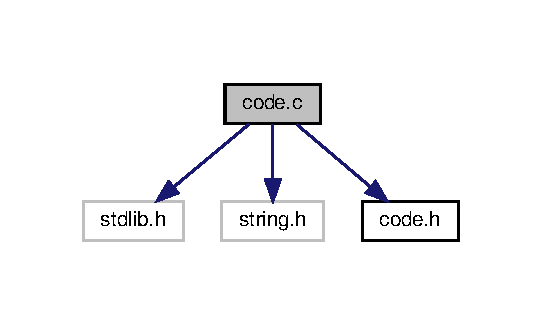
\includegraphics[width=260pt]{code_8c__incl}
\end{center}
\end{figure}
\subsection*{Functions}
\begin{DoxyCompactItemize}
\item 
char $\ast$ \hyperlink{code_8c_a8d64bc3ec5de4db181efd7ff565ff894}{translate\+Seq} (char $\ast$seq)
\item 
int $\ast$ \hyperlink{code_8c_a011bbc41b53a2519b2bb46214b7a1fcc}{encode\+Seq} (char $\ast$seq)
\item 
int \hyperlink{code_8c_a617a88955038003d70de0d9113b505eb}{encode\+AA} (char aa)
\item 
char \hyperlink{code_8c_a124646f7d65dd512584b8fbab1fcc7a4}{decode\+AA} (int encoded\+AA)
\end{DoxyCompactItemize}
\subsection*{Variables}
\begin{DoxyCompactItemize}
\item 
int \hyperlink{code_8c_a119a7eb0ecd417f83e41f4325ce522c8}{transcode} \mbox{[}4\mbox{]}\mbox{[}4\mbox{]}\mbox{[}4\mbox{]}
\item 
int \hyperlink{code_8c_a528f2f941a2c7a8de187c946e438d107}{B\+L\+O\+S\+U\+M62} \mbox{[}24\mbox{]}\mbox{[}24\mbox{]}
\item 
int \hyperlink{code_8c_addcd68ee32c359359fcb55b5bfd8a62f}{B\+L\+O\+S\+U\+M90} \mbox{[}24\mbox{]}\mbox{[}24\mbox{]}
\end{DoxyCompactItemize}


\subsection{Function Documentation}
\mbox{\Hypertarget{code_8c_a124646f7d65dd512584b8fbab1fcc7a4}\label{code_8c_a124646f7d65dd512584b8fbab1fcc7a4}} 
\index{code.\+c@{code.\+c}!decode\+AA@{decode\+AA}}
\index{decode\+AA@{decode\+AA}!code.\+c@{code.\+c}}
\subsubsection{\texorpdfstring{decode\+A\+A()}{decodeAA()}}
{\footnotesize\ttfamily char decode\+AA (\begin{DoxyParamCaption}\item[{int}]{encoded\+AA }\end{DoxyParamCaption})}

\mbox{\Hypertarget{code_8c_a617a88955038003d70de0d9113b505eb}\label{code_8c_a617a88955038003d70de0d9113b505eb}} 
\index{code.\+c@{code.\+c}!encode\+AA@{encode\+AA}}
\index{encode\+AA@{encode\+AA}!code.\+c@{code.\+c}}
\subsubsection{\texorpdfstring{encode\+A\+A()}{encodeAA()}}
{\footnotesize\ttfamily int encode\+AA (\begin{DoxyParamCaption}\item[{char}]{aa }\end{DoxyParamCaption})}

\mbox{\Hypertarget{code_8c_a011bbc41b53a2519b2bb46214b7a1fcc}\label{code_8c_a011bbc41b53a2519b2bb46214b7a1fcc}} 
\index{code.\+c@{code.\+c}!encode\+Seq@{encode\+Seq}}
\index{encode\+Seq@{encode\+Seq}!code.\+c@{code.\+c}}
\subsubsection{\texorpdfstring{encode\+Seq()}{encodeSeq()}}
{\footnotesize\ttfamily int$\ast$ encode\+Seq (\begin{DoxyParamCaption}\item[{char $\ast$}]{seq }\end{DoxyParamCaption})}

\mbox{\Hypertarget{code_8c_a8d64bc3ec5de4db181efd7ff565ff894}\label{code_8c_a8d64bc3ec5de4db181efd7ff565ff894}} 
\index{code.\+c@{code.\+c}!translate\+Seq@{translate\+Seq}}
\index{translate\+Seq@{translate\+Seq}!code.\+c@{code.\+c}}
\subsubsection{\texorpdfstring{translate\+Seq()}{translateSeq()}}
{\footnotesize\ttfamily char$\ast$ translate\+Seq (\begin{DoxyParamCaption}\item[{char $\ast$}]{seq }\end{DoxyParamCaption})}

Here is the call graph for this function\+:
\nopagebreak
\begin{figure}[H]
\begin{center}
\leavevmode
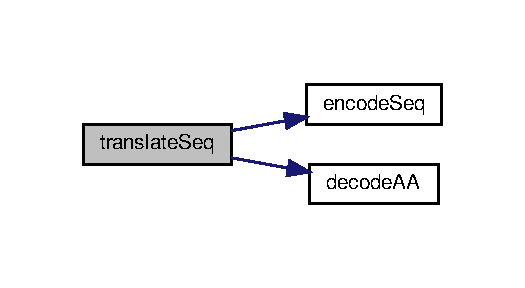
\includegraphics[width=252pt]{code_8c_a8d64bc3ec5de4db181efd7ff565ff894_cgraph}
\end{center}
\end{figure}


\subsection{Variable Documentation}
\mbox{\Hypertarget{code_8c_a528f2f941a2c7a8de187c946e438d107}\label{code_8c_a528f2f941a2c7a8de187c946e438d107}} 
\index{code.\+c@{code.\+c}!B\+L\+O\+S\+U\+M62@{B\+L\+O\+S\+U\+M62}}
\index{B\+L\+O\+S\+U\+M62@{B\+L\+O\+S\+U\+M62}!code.\+c@{code.\+c}}
\subsubsection{\texorpdfstring{B\+L\+O\+S\+U\+M62}{BLOSUM62}}
{\footnotesize\ttfamily int B\+L\+O\+S\+U\+M62\mbox{[}24\mbox{]}\mbox{[}24\mbox{]}}

{\bfseries Initial value\+:}
\begin{DoxyCode}
=\{\{ 4,-1,-2,-2, 0,-1,-1, 0,-2,-1,-1,-1,-1,-2,-1, 1, 0,-3,-2, 0,-2,-1, 0,-4\},
                      \{-1, 5, 0,-2,-3, 1, 0,-2, 0,-3,-2, 2,-1,-3,-2,-1,-1,-3,-2,-3,-1, 0,-1,-4\},
                      \{-2, 0, 6, 1,-3, 0, 0, 0, 1,-3,-3, 0,-2,-3,-2, 1, 0,-4,-2,-3, 3, 0,-1,-4\},
                      \{-2,-2, 1, 6,-3, 0, 2,-1,-1,-3,-4,-1,-3,-3,-1, 0,-1,-4,-3,-3, 4, 1,-1,-4\},
                      \{ 0,-3,-3,-3, 9,-3,-4,-3,-3,-1,-1,-3,-1,-2,-3,-1,-1,-2,-2,-1,-3,-3,-2,-4\},
                      \{-1, 1, 0, 0,-3, 5, 2,-2, 0,-3,-2, 1, 0,-3,-1, 0,-1,-2,-1,-2, 0, 3,-1,-4\},
                      \{-1, 0, 0, 2,-4, 2, 5,-2, 0,-3,-3, 1,-2,-3,-1, 0,-1,-3,-2,-2, 1, 4,-1,-4\},
                      \{ 0,-2, 0,-1,-3,-2,-2, 6,-2,-4,-4,-2,-3,-3,-2, 0,-2,-2,-3,-3,-1,-2,-1,-4\},
                      \{-2, 0, 1,-1,-3, 0, 0,-2, 8,-3,-3,-1,-2,-1,-2,-1,-2,-2, 2,-3, 0, 0,-1,-4\},
                      \{-1,-3,-3,-3,-1,-3,-3,-4,-3, 4, 2,-3, 1, 0,-3,-2,-1,-3,-1, 3,-3,-3,-1,-4\},
                      \{-1,-2,-3,-4,-1,-2,-3,-4,-3, 2, 4,-2, 2, 0,-3,-2,-1,-2,-1, 1,-4,-3,-1,-4\},
                      \{-1, 2, 0,-1,-3, 1, 1,-2,-1,-3,-2, 5,-1,-3,-1, 0,-1,-3,-2,-2, 0, 1,-1,-4\},
                      \{-1,-1,-2,-3,-1, 0,-2,-3,-2, 1, 2,-1, 5, 0,-2,-1,-1,-1,-1, 1,-3,-1,-1,-4\},
                      \{-2,-3,-3,-3,-2,-3,-3,-3,-1, 0, 0,-3, 0, 6,-4,-2,-2, 1, 3,-1,-3,-3,-1,-4\},
                      \{-1,-2,-2,-1,-3,-1,-1,-2,-2,-3,-3,-1,-2,-4, 7,-1,-1,-4,-3,-2,-2,-1,-2,-4\},
                      \{ 1,-1, 1, 0,-1, 0, 0, 0,-1,-2,-2, 0,-1,-2,-1, 4, 1,-3,-2,-2, 0, 0, 0,-4\},
                      \{ 0,-1, 0,-1,-1,-1,-1,-2,-2,-1,-1,-1,-1,-2,-1, 1, 5,-2,-2, 0,-1,-1, 0,-4\},
                      \{-3,-3,-4,-4,-2,-2,-3,-2,-2,-3,-2,-3,-1, 1,-4,-3,-2, 11, 2,-3,-4,-3,-2,-4\},
                      \{-2,-2,-2,-3,-2,-1,-2,-3, 2,-1,-1,-2,-1, 3,-3,-2,-2, 2, 7,-1,-3,-2,-1,-4\},
                      \{ 0,-3,-3,-3,-1,-2,-2,-3,-3, 3, 1,-2, 1,-1,-2,-2, 0,-3,-1, 4,-3,-2,-1,-4\},
                      \{-2,-1, 3, 4,-3, 0, 1,-1, 0,-3,-4, 0,-3,-3,-2, 0,-1,-4,-3,-3, 4, 1,-1,-4\},
                      \{-1, 0, 0, 1,-3, 3, 4,-2, 0,-3,-3, 1,-1,-3,-1, 0,-1,-3,-2,-2, 1, 4,-1,-4\},
                      \{ 0,-1,-1,-1,-2,-1,-1,-1,-1,-1,-1,-1,-1,-1,-2, 0, 0,-2,-1,-1,-1,-1,-1,-4\},
                      \{-4,-4,-4,-4,-4,-4,-4,-4,-4,-4,-4,-4,-4,-4,-4,-4,-4,-4,-4,-4,-4,-4,-4, 1\}\}
\end{DoxyCode}
\mbox{\Hypertarget{code_8c_addcd68ee32c359359fcb55b5bfd8a62f}\label{code_8c_addcd68ee32c359359fcb55b5bfd8a62f}} 
\index{code.\+c@{code.\+c}!B\+L\+O\+S\+U\+M90@{B\+L\+O\+S\+U\+M90}}
\index{B\+L\+O\+S\+U\+M90@{B\+L\+O\+S\+U\+M90}!code.\+c@{code.\+c}}
\subsubsection{\texorpdfstring{B\+L\+O\+S\+U\+M90}{BLOSUM90}}
{\footnotesize\ttfamily int B\+L\+O\+S\+U\+M90\mbox{[}24\mbox{]}\mbox{[}24\mbox{]}}

{\bfseries Initial value\+:}
\begin{DoxyCode}
=\{\{ 5,-2,-2,-3,-1,-1,-1, 0,-2,-2,-2,-1,-2,-3,-1, 1, 0,-4,-3,-1,-2,-1,-1,-6\},
                      \{-2, 6,-1,-3,-5, 1,-1,-3, 0,-4,-3, 2,-2,-4,-3,-1,-2,-4,-3,-3,-2, 0,-2,-6\},
                      \{-2,-1, 7, 1,-4, 0,-1,-1, 0,-4,-4, 0,-3,-4,-3, 0, 0,-5,-3,-4, 4,-1,-2,-6\},
                      \{-3,-3, 1, 7,-5,-1, 1,-2,-2,-5,-5,-1,-4,-5,-3,-1,-2,-6,-4,-5, 4, 0,-2,-6\},
                      \{-1,-5,-4,-5, 9,-4,-6,-4,-5,-2,-2,-4,-2,-3,-4,-2,-2,-4,-4,-2,-4,-5,-3,-6\},
                      \{-1, 1, 0,-1,-4, 7, 2,-3, 1,-4,-3, 1, 0,-4,-2,-1,-1,-3,-3,-3,-1, 4,-1,-6\},
                      \{-1,-1,-1, 1,-6, 2, 6,-3,-1,-4,-4, 0,-3,-5,-2,-1,-1,-5,-4,-3, 0, 4,-2,-6\},
                      \{ 0,-3,-1,-2,-4,-3,-3, 6,-3,-5,-5,-2,-4,-5,-3,-1,-3,-4,-5,-5,-2,-3,-2,-6\},
                      \{-2, 0, 0,-2,-5, 1,-1,-3, 8,-4,-4,-1,-3,-2,-3,-2,-2,-3, 1,-4,-1, 0,-2,-6\},
                      \{-2,-4,-4,-5,-2,-4,-4,-5,-4, 5, 1,-4, 1,-1,-4,-3,-1,-4,-2, 3,-5,-4,-2,-6\},
                      \{-2,-3,-4,-5,-2,-3,-4,-5,-4, 1, 5,-3, 2, 0,-4,-3,-2,-3,-2, 0,-5,-4,-2,-6\},
                      \{-1, 2, 0,-1,-4, 1, 0,-2,-1,-4,-3, 6,-2,-4,-2,-1,-1,-5,-3,-3,-1, 1,-1,-6\},
                      \{-2,-2,-3,-4,-2, 0,-3,-4,-3, 1, 2,-2, 7,-1,-3,-2,-1,-2,-2, 0,-4,-2,-1,-6\},
                      \{-3,-4,-4,-5,-3,-4,-5,-5,-2,-1, 0,-4,-1, 7,-4,-3,-3, 0, 3,-2,-4,-4,-2,-6\},
                      \{-1,-3,-3,-3,-4,-2,-2,-3,-3,-4,-4,-2,-3,-4, 8,-2,-2,-5,-4,-3,-3,-2,-2,-6\},
                      \{ 1,-1, 0,-1,-2,-1,-1,-1,-2,-3,-3,-1,-2,-3,-2, 5, 1,-4,-3,-2, 0,-1,-1,-6\},
                      \{ 0,-2, 0,-2,-2,-1,-1,-3,-2,-1,-2,-1,-1,-3,-2, 1, 6,-4,-2,-1,-1,-1,-1,-6\},
                      \{-4,-4,-5,-6,-4,-3,-5,-4,-3,-4,-3,-5,-2, 0,-5,-4,-4, 11, 2,-3,-6,-4,-3,-6\},
                      \{-3,-3,-3,-4,-4,-3,-4,-5, 1,-2,-2,-3,-2, 3,-4,-3,-2, 2, 8,-3,-4,-3,-2,-6\},
                      \{-1,-3,-4,-5,-2,-3,-3,-5,-4, 3, 0,-3, 0,-2,-3,-2,-1,-3,-3, 5,-4,-3,-2,-6\},
                      \{-2,-2, 4, 4,-4,-1, 0,-2,-1,-5,-5,-1,-4,-4,-3, 0,-1,-6,-4,-4, 4, 0,-2,-6\},
                      \{-1, 0,-1, 0,-5, 4, 4,-3, 0,-4,-4, 1,-2,-4,-2,-1,-1,-4,-3,-3, 0, 4,-1,-6\},
                      \{-1,-2,-2,-2,-3,-1,-2,-2,-2,-2,-2,-1,-1,-2,-2,-1,-1,-3,-2,-2,-2,-1,-2,-6\},
                      \{-6,-6,-6,-6,-6,-6,-6,-6,-6,-6,-6,-6,-6,-6,-6,-6,-6,-6,-6,-6,-6,-6,-6, 1\},
\}
\end{DoxyCode}
\mbox{\Hypertarget{code_8c_a119a7eb0ecd417f83e41f4325ce522c8}\label{code_8c_a119a7eb0ecd417f83e41f4325ce522c8}} 
\index{code.\+c@{code.\+c}!transcode@{transcode}}
\index{transcode@{transcode}!code.\+c@{code.\+c}}
\subsubsection{\texorpdfstring{transcode}{transcode}}
{\footnotesize\ttfamily int transcode\mbox{[}4\mbox{]}\mbox{[}4\mbox{]}\mbox{[}4\mbox{]}}

{\bfseries Initial value\+:}
\begin{DoxyCode}
=\{\{\{ 11, 2 , 11, 2 \},\{ 16, 16, 16, 16\},\{ 1 , 15, 1 , 15\},\{ 9 , 9 , 12, 9 \}\},
  

                        \{\{ 5 , 8 , 5 , 8 \},\{ 14, 14, 14, 14\},\{ 1 , 1 , 1 , 1 \},\{ 10, 10, 10, 10 \}\},
  

                        \{\{ 6 , 3 , 6 , 3 \},\{ 0 , 0 , 0 , 0 \},\{ 7 , 7 , 7 , 7 \},\{ 19, 19, 19, 19\}\},

  
                        \{\{ -1, 18, -1, 18\},\{ 15, 15, 15, 15\},\{ -1, 4 , 17, 4 \},\{ 10, 13, 10, 13\}\}\}
\end{DoxyCode}

\hypertarget{code_8h}{}\section{code.\+h File Reference}
\label{code_8h}\index{code.\+h@{code.\+h}}
This graph shows which files directly or indirectly include this file\+:
\nopagebreak
\begin{figure}[H]
\begin{center}
\leavevmode
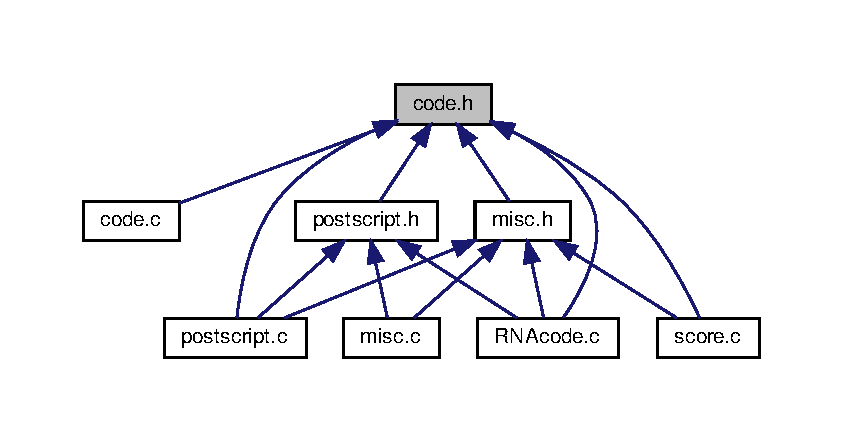
\includegraphics[width=350pt]{code_8h__dep__incl}
\end{center}
\end{figure}
\subsection*{Functions}
\begin{DoxyCompactItemize}
\item 
int $\ast$ \hyperlink{code_8h_a011bbc41b53a2519b2bb46214b7a1fcc}{encode\+Seq} (char $\ast$seq)
\item 
int \hyperlink{code_8h_a617a88955038003d70de0d9113b505eb}{encode\+AA} (char aa)
\item 
char \hyperlink{code_8h_a124646f7d65dd512584b8fbab1fcc7a4}{decode\+AA} (int encoded\+AA)
\item 
char $\ast$ \hyperlink{code_8h_a8d64bc3ec5de4db181efd7ff565ff894}{translate\+Seq} (char $\ast$seq)
\end{DoxyCompactItemize}


\subsection{Function Documentation}
\mbox{\Hypertarget{code_8h_a124646f7d65dd512584b8fbab1fcc7a4}\label{code_8h_a124646f7d65dd512584b8fbab1fcc7a4}} 
\index{code.\+h@{code.\+h}!decode\+AA@{decode\+AA}}
\index{decode\+AA@{decode\+AA}!code.\+h@{code.\+h}}
\subsubsection{\texorpdfstring{decode\+A\+A()}{decodeAA()}}
{\footnotesize\ttfamily char decode\+AA (\begin{DoxyParamCaption}\item[{int}]{encoded\+AA }\end{DoxyParamCaption})}

\mbox{\Hypertarget{code_8h_a617a88955038003d70de0d9113b505eb}\label{code_8h_a617a88955038003d70de0d9113b505eb}} 
\index{code.\+h@{code.\+h}!encode\+AA@{encode\+AA}}
\index{encode\+AA@{encode\+AA}!code.\+h@{code.\+h}}
\subsubsection{\texorpdfstring{encode\+A\+A()}{encodeAA()}}
{\footnotesize\ttfamily int encode\+AA (\begin{DoxyParamCaption}\item[{char}]{aa }\end{DoxyParamCaption})}

\mbox{\Hypertarget{code_8h_a011bbc41b53a2519b2bb46214b7a1fcc}\label{code_8h_a011bbc41b53a2519b2bb46214b7a1fcc}} 
\index{code.\+h@{code.\+h}!encode\+Seq@{encode\+Seq}}
\index{encode\+Seq@{encode\+Seq}!code.\+h@{code.\+h}}
\subsubsection{\texorpdfstring{encode\+Seq()}{encodeSeq()}}
{\footnotesize\ttfamily int$\ast$ encode\+Seq (\begin{DoxyParamCaption}\item[{char $\ast$}]{seq }\end{DoxyParamCaption})}

\mbox{\Hypertarget{code_8h_a8d64bc3ec5de4db181efd7ff565ff894}\label{code_8h_a8d64bc3ec5de4db181efd7ff565ff894}} 
\index{code.\+h@{code.\+h}!translate\+Seq@{translate\+Seq}}
\index{translate\+Seq@{translate\+Seq}!code.\+h@{code.\+h}}
\subsubsection{\texorpdfstring{translate\+Seq()}{translateSeq()}}
{\footnotesize\ttfamily char$\ast$ translate\+Seq (\begin{DoxyParamCaption}\item[{char $\ast$}]{seq }\end{DoxyParamCaption})}

Here is the call graph for this function\+:
\nopagebreak
\begin{figure}[H]
\begin{center}
\leavevmode
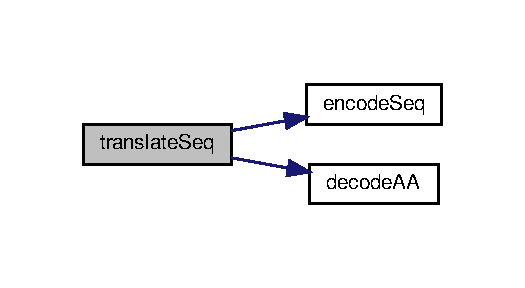
\includegraphics[width=252pt]{code_8h_a8d64bc3ec5de4db181efd7ff565ff894_cgraph}
\end{center}
\end{figure}

\hypertarget{extreme__fit_8c}{}\section{extreme\+\_\+fit.\+c File Reference}
\label{extreme__fit_8c}\index{extreme\+\_\+fit.\+c@{extreme\+\_\+fit.\+c}}
{\ttfamily \#include $<$stdlib.\+h$>$}\newline
{\ttfamily \#include $<$stdio.\+h$>$}\newline
{\ttfamily \#include $<$math.\+h$>$}\newline
{\ttfamily \#include \char`\"{}extreme\+\_\+fit.\+h\char`\"{}}\newline
{\ttfamily \#include \char`\"{}lm.\+h\char`\"{}}\newline
Include dependency graph for extreme\+\_\+fit.\+c\+:
\nopagebreak
\begin{figure}[H]
\begin{center}
\leavevmode
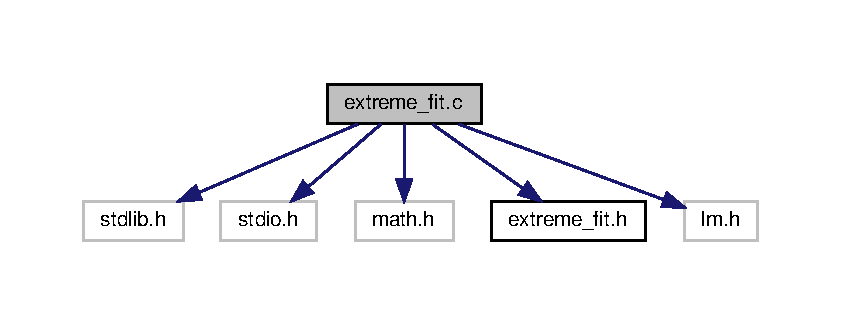
\includegraphics[width=350pt]{extreme__fit_8c__incl}
\end{center}
\end{figure}
\subsection*{Functions}
\begin{DoxyCompactItemize}
\item 
void \hyperlink{extreme__fit_8c_ac7d28c2cfa789de3864ed5d07ef800ec}{Lawless416} (double $\ast$x, int $\ast$y, int n, double lambda, double $\ast$ret\+\_\+f, double $\ast$ret\+\_\+df)
\item 
void \hyperlink{extreme__fit_8c_a05c76c8801e372734c3888b165c28f86}{Lawless422} (double $\ast$x, int $\ast$y, int n, int z, double c, double lambda, double $\ast$ret\+\_\+f, double $\ast$ret\+\_\+df)
\item 
int \hyperlink{extreme__fit_8c_a51c7409c6447353e0bd3b7c48d982984}{E\+V\+D\+Max\+Likely\+Fit} (double $\ast$x, int $\ast$c, int n, double $\ast$ret\+\_\+mu, double $\ast$ret\+\_\+lambda)
\end{DoxyCompactItemize}


\subsection{Function Documentation}
\mbox{\Hypertarget{extreme__fit_8c_a51c7409c6447353e0bd3b7c48d982984}\label{extreme__fit_8c_a51c7409c6447353e0bd3b7c48d982984}} 
\index{extreme\+\_\+fit.\+c@{extreme\+\_\+fit.\+c}!E\+V\+D\+Max\+Likely\+Fit@{E\+V\+D\+Max\+Likely\+Fit}}
\index{E\+V\+D\+Max\+Likely\+Fit@{E\+V\+D\+Max\+Likely\+Fit}!extreme\+\_\+fit.\+c@{extreme\+\_\+fit.\+c}}
\subsubsection{\texorpdfstring{E\+V\+D\+Max\+Likely\+Fit()}{EVDMaxLikelyFit()}}
{\footnotesize\ttfamily int E\+V\+D\+Max\+Likely\+Fit (\begin{DoxyParamCaption}\item[{double $\ast$}]{x,  }\item[{int $\ast$}]{c,  }\item[{int}]{n,  }\item[{double $\ast$}]{ret\+\_\+mu,  }\item[{double $\ast$}]{ret\+\_\+lambda }\end{DoxyParamCaption})}

Here is the call graph for this function\+:
\nopagebreak
\begin{figure}[H]
\begin{center}
\leavevmode
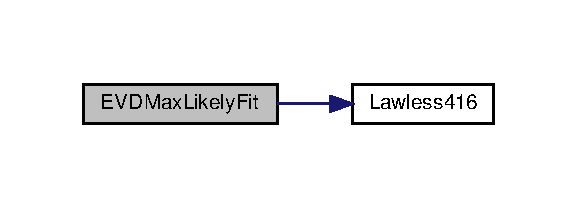
\includegraphics[width=277pt]{extreme__fit_8c_a51c7409c6447353e0bd3b7c48d982984_cgraph}
\end{center}
\end{figure}
\mbox{\Hypertarget{extreme__fit_8c_ac7d28c2cfa789de3864ed5d07ef800ec}\label{extreme__fit_8c_ac7d28c2cfa789de3864ed5d07ef800ec}} 
\index{extreme\+\_\+fit.\+c@{extreme\+\_\+fit.\+c}!Lawless416@{Lawless416}}
\index{Lawless416@{Lawless416}!extreme\+\_\+fit.\+c@{extreme\+\_\+fit.\+c}}
\subsubsection{\texorpdfstring{Lawless416()}{Lawless416()}}
{\footnotesize\ttfamily void Lawless416 (\begin{DoxyParamCaption}\item[{double $\ast$}]{x,  }\item[{int $\ast$}]{y,  }\item[{int}]{n,  }\item[{double}]{lambda,  }\item[{double $\ast$}]{ret\+\_\+f,  }\item[{double $\ast$}]{ret\+\_\+df }\end{DoxyParamCaption})}

\mbox{\Hypertarget{extreme__fit_8c_a05c76c8801e372734c3888b165c28f86}\label{extreme__fit_8c_a05c76c8801e372734c3888b165c28f86}} 
\index{extreme\+\_\+fit.\+c@{extreme\+\_\+fit.\+c}!Lawless422@{Lawless422}}
\index{Lawless422@{Lawless422}!extreme\+\_\+fit.\+c@{extreme\+\_\+fit.\+c}}
\subsubsection{\texorpdfstring{Lawless422()}{Lawless422()}}
{\footnotesize\ttfamily void Lawless422 (\begin{DoxyParamCaption}\item[{double $\ast$}]{x,  }\item[{int $\ast$}]{y,  }\item[{int}]{n,  }\item[{int}]{z,  }\item[{double}]{c,  }\item[{double}]{lambda,  }\item[{double $\ast$}]{ret\+\_\+f,  }\item[{double $\ast$}]{ret\+\_\+df }\end{DoxyParamCaption})}


\hypertarget{extreme__fit_8h}{}\section{extreme\+\_\+fit.\+h File Reference}
\label{extreme__fit_8h}\index{extreme\+\_\+fit.\+h@{extreme\+\_\+fit.\+h}}
This graph shows which files directly or indirectly include this file\+:
\nopagebreak
\begin{figure}[H]
\begin{center}
\leavevmode
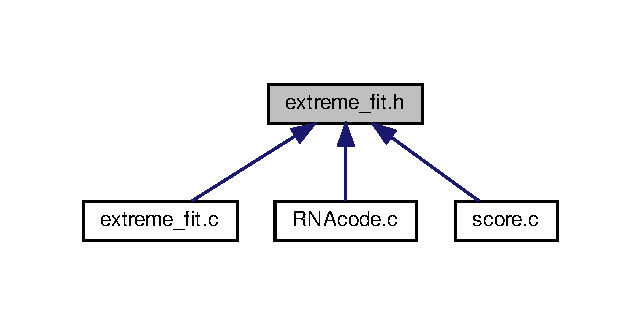
\includegraphics[width=308pt]{extreme__fit_8h__dep__incl}
\end{center}
\end{figure}
\subsection*{Functions}
\begin{DoxyCompactItemize}
\item 
int \hyperlink{extreme__fit_8h_a51c7409c6447353e0bd3b7c48d982984}{E\+V\+D\+Max\+Likely\+Fit} (double $\ast$x, int $\ast$c, int n, double $\ast$ret\+\_\+mu, double $\ast$ret\+\_\+lambda)
\end{DoxyCompactItemize}


\subsection{Function Documentation}
\mbox{\Hypertarget{extreme__fit_8h_a51c7409c6447353e0bd3b7c48d982984}\label{extreme__fit_8h_a51c7409c6447353e0bd3b7c48d982984}} 
\index{extreme\+\_\+fit.\+h@{extreme\+\_\+fit.\+h}!E\+V\+D\+Max\+Likely\+Fit@{E\+V\+D\+Max\+Likely\+Fit}}
\index{E\+V\+D\+Max\+Likely\+Fit@{E\+V\+D\+Max\+Likely\+Fit}!extreme\+\_\+fit.\+h@{extreme\+\_\+fit.\+h}}
\subsubsection{\texorpdfstring{E\+V\+D\+Max\+Likely\+Fit()}{EVDMaxLikelyFit()}}
{\footnotesize\ttfamily int E\+V\+D\+Max\+Likely\+Fit (\begin{DoxyParamCaption}\item[{double $\ast$}]{x,  }\item[{int $\ast$}]{c,  }\item[{int}]{n,  }\item[{double $\ast$}]{ret\+\_\+mu,  }\item[{double $\ast$}]{ret\+\_\+lambda }\end{DoxyParamCaption})}

Here is the call graph for this function\+:
\nopagebreak
\begin{figure}[H]
\begin{center}
\leavevmode
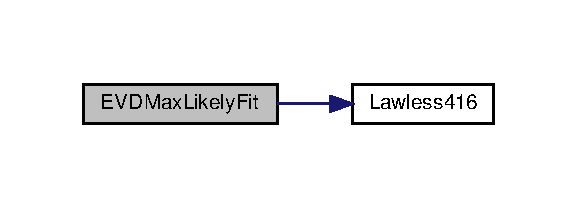
\includegraphics[width=277pt]{extreme__fit_8h_a51c7409c6447353e0bd3b7c48d982984_cgraph}
\end{center}
\end{figure}

\hypertarget{getopt_8c}{}\section{getopt.\+c File Reference}
\label{getopt_8c}\index{getopt.\+c@{getopt.\+c}}
{\ttfamily \#include $<$stdio.\+h$>$}\newline
{\ttfamily \#include \char`\"{}getopt.\+h\char`\"{}}\newline
{\ttfamily \#include $<$strings.\+h$>$}\newline
Include dependency graph for getopt.\+c\+:
\nopagebreak
\begin{figure}[H]
\begin{center}
\leavevmode
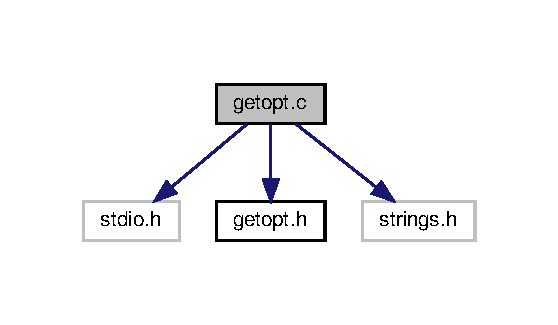
\includegraphics[width=268pt]{getopt_8c__incl}
\end{center}
\end{figure}
\subsection*{Macros}
\begin{DoxyCompactItemize}
\item 
\#define \hyperlink{getopt_8c_a9bcd7db9771ff03b7e5a9fec9c489861}{\+\_\+\+N\+O\+\_\+\+P\+R\+O\+TO}
\item 
\#define \hyperlink{getopt_8c_a2c212835823e3c54a8ab6d95c652660e}{const}
\item 
\#define \hyperlink{getopt_8c_a5325c715897861c318d3ae312ac452cc}{G\+E\+T\+O\+P\+T\+\_\+\+I\+N\+T\+E\+R\+F\+A\+C\+E\+\_\+\+V\+E\+R\+S\+I\+ON}~2
\item 
\#define \hyperlink{getopt_8c_a86a239addea586602343007a370bf8ad}{\+\_\+}(msgid)~(msgid)
\item 
\#define \hyperlink{getopt_8c_a6e06e56c5fa96faaf47f3b231e015e35}{S\+W\+A\+P\+\_\+\+F\+L\+A\+GS}(ch1,  ch2)
\item 
\#define \hyperlink{getopt_8c_a71ceb8911d64b39b402041ba5ea8453c}{N\+O\+N\+O\+P\+T\+I\+O\+N\+\_\+P}~(argv\mbox{[}\hyperlink{getopt_8h_ad5e1c16213bbee2d5e8cc363309f418c}{optind}\mbox{]}\mbox{[}0\mbox{]} != \textquotesingle{}-\/\textquotesingle{} $\vert$$\vert$ argv\mbox{[}\hyperlink{getopt_8h_ad5e1c16213bbee2d5e8cc363309f418c}{optind}\mbox{]}\mbox{[}1\mbox{]} == \textquotesingle{}\textbackslash{}0\textquotesingle{})
\end{DoxyCompactItemize}
\subsection*{Enumerations}
\begin{DoxyCompactItemize}
\item 
enum \{ \hyperlink{getopt_8c_a06fc87d81c62e9abb8790b6e5713c55ba0e73a0691c110b1442d8364d1d12eccc}{R\+E\+Q\+U\+I\+R\+E\+\_\+\+O\+R\+D\+ER}, 
\hyperlink{getopt_8c_a06fc87d81c62e9abb8790b6e5713c55bacfdde4b47c27f4efbd832e1ac7f8a8fc}{P\+E\+R\+M\+U\+TE}, 
\hyperlink{getopt_8c_a06fc87d81c62e9abb8790b6e5713c55ba3c56550bfafe809d9214b863b69c31c5}{R\+E\+T\+U\+R\+N\+\_\+\+I\+N\+\_\+\+O\+R\+D\+ER}
 \}
\end{DoxyCompactItemize}
\subsection*{Functions}
\begin{DoxyCompactItemize}
\item 
char $\ast$ \hyperlink{getopt_8c_aee28fd8a0e40b6d958f7d20348e45368}{getenv} ()
\item 
static char $\ast$ \hyperlink{getopt_8c_ae0ac978b7775f69496c0f127ffdada9d}{my\+\_\+index} (char $\ast$str, int chr) \hyperlink{getopt_8c_a2c212835823e3c54a8ab6d95c652660e}{const}
\item 
static void \hyperlink{getopt_8c_a4621659dd6377e52ac50a0869625bb6e}{exchange} (char $\ast$$\ast$argv)
\item 
static \hyperlink{getopt_8c_a2c212835823e3c54a8ab6d95c652660e}{const} char $\ast$ \hyperlink{getopt_8c_a17475cbc1ffae0c12af2e0a3319d197f}{\+\_\+getopt\+\_\+initialize} (int argc, char $\ast$\hyperlink{getopt_8c_a2c212835823e3c54a8ab6d95c652660e}{const} $\ast$argv, \hyperlink{getopt_8c_a2c212835823e3c54a8ab6d95c652660e}{const} char $\ast$optstring)
\item 
int \hyperlink{getopt_8c_a0df92a0ae8fe1fd43268c738f548674f}{\+\_\+getopt\+\_\+internal} (int argc, char $\ast$\hyperlink{getopt_8c_a2c212835823e3c54a8ab6d95c652660e}{const} $\ast$argv, \hyperlink{getopt_8c_a2c212835823e3c54a8ab6d95c652660e}{const} char $\ast$optstring, \hyperlink{getopt_8c_a2c212835823e3c54a8ab6d95c652660e}{const} struct \hyperlink{structoption}{option} $\ast$longopts, int $\ast$longind, int long\+\_\+only)
\item 
int \hyperlink{getopt_8c_a1b2ada39ab92162c6ec9c67c8093fa2e}{getopt} (int argc, char $\ast$\hyperlink{getopt_8c_a2c212835823e3c54a8ab6d95c652660e}{const} $\ast$argv, \hyperlink{getopt_8c_a2c212835823e3c54a8ab6d95c652660e}{const} char $\ast$optstring)
\end{DoxyCompactItemize}
\subsection*{Variables}
\begin{DoxyCompactItemize}
\item 
char $\ast$ \hyperlink{getopt_8c_adb50a0eab9fed92fc3bfc7dfa4f2c410}{optarg}
\item 
int \hyperlink{getopt_8c_ad5e1c16213bbee2d5e8cc363309f418c}{optind} = 1
\item 
int \hyperlink{getopt_8c_a28286be757527aeb1db951b5da9aeec1}{\+\_\+\+\_\+getopt\+\_\+initialized}
\item 
static char $\ast$ \hyperlink{getopt_8c_a47a40a4c365dae45f94751ad32aab530}{nextchar}
\item 
int \hyperlink{getopt_8c_ae30f05ee1e2e5652f174a35c7875d25e}{opterr} = 1
\item 
int \hyperlink{getopt_8c_a475b8db98445da73e5f62a1ef6324b95}{optopt} = \textquotesingle{}?\textquotesingle{}
\item 
static enum  \{ ... \}  \hyperlink{getopt_8c_a67a84cf4dacaa8337be68345f8b9a8cc}{ordering}
\item 
static char $\ast$ \hyperlink{getopt_8c_ad0ccb64bbd4defe7a57dbad2045ddd14}{posixly\+\_\+correct}
\item 
static int \hyperlink{getopt_8c_a7b0f4f3bfbee147113f282427ce933ed}{first\+\_\+nonopt}
\item 
static int \hyperlink{getopt_8c_a580f2c2acf35dad51ca18b427212bf15}{last\+\_\+nonopt}
\end{DoxyCompactItemize}


\subsection{Macro Definition Documentation}
\mbox{\Hypertarget{getopt_8c_a86a239addea586602343007a370bf8ad}\label{getopt_8c_a86a239addea586602343007a370bf8ad}} 
\index{getopt.\+c@{getopt.\+c}!\+\_\+@{\+\_\+}}
\index{\+\_\+@{\+\_\+}!getopt.\+c@{getopt.\+c}}
\subsubsection{\texorpdfstring{\+\_\+}{\_}}
{\footnotesize\ttfamily \#define \+\_\+(\begin{DoxyParamCaption}\item[{}]{msgid }\end{DoxyParamCaption})~(msgid)}

\mbox{\Hypertarget{getopt_8c_a9bcd7db9771ff03b7e5a9fec9c489861}\label{getopt_8c_a9bcd7db9771ff03b7e5a9fec9c489861}} 
\index{getopt.\+c@{getopt.\+c}!\+\_\+\+N\+O\+\_\+\+P\+R\+O\+TO@{\+\_\+\+N\+O\+\_\+\+P\+R\+O\+TO}}
\index{\+\_\+\+N\+O\+\_\+\+P\+R\+O\+TO@{\+\_\+\+N\+O\+\_\+\+P\+R\+O\+TO}!getopt.\+c@{getopt.\+c}}
\subsubsection{\texorpdfstring{\+\_\+\+N\+O\+\_\+\+P\+R\+O\+TO}{\_NO\_PROTO}}
{\footnotesize\ttfamily \#define \+\_\+\+N\+O\+\_\+\+P\+R\+O\+TO}

\mbox{\Hypertarget{getopt_8c_a2c212835823e3c54a8ab6d95c652660e}\label{getopt_8c_a2c212835823e3c54a8ab6d95c652660e}} 
\index{getopt.\+c@{getopt.\+c}!const@{const}}
\index{const@{const}!getopt.\+c@{getopt.\+c}}
\subsubsection{\texorpdfstring{const}{const}}
{\footnotesize\ttfamily \#define const}

\mbox{\Hypertarget{getopt_8c_a5325c715897861c318d3ae312ac452cc}\label{getopt_8c_a5325c715897861c318d3ae312ac452cc}} 
\index{getopt.\+c@{getopt.\+c}!G\+E\+T\+O\+P\+T\+\_\+\+I\+N\+T\+E\+R\+F\+A\+C\+E\+\_\+\+V\+E\+R\+S\+I\+ON@{G\+E\+T\+O\+P\+T\+\_\+\+I\+N\+T\+E\+R\+F\+A\+C\+E\+\_\+\+V\+E\+R\+S\+I\+ON}}
\index{G\+E\+T\+O\+P\+T\+\_\+\+I\+N\+T\+E\+R\+F\+A\+C\+E\+\_\+\+V\+E\+R\+S\+I\+ON@{G\+E\+T\+O\+P\+T\+\_\+\+I\+N\+T\+E\+R\+F\+A\+C\+E\+\_\+\+V\+E\+R\+S\+I\+ON}!getopt.\+c@{getopt.\+c}}
\subsubsection{\texorpdfstring{G\+E\+T\+O\+P\+T\+\_\+\+I\+N\+T\+E\+R\+F\+A\+C\+E\+\_\+\+V\+E\+R\+S\+I\+ON}{GETOPT\_INTERFACE\_VERSION}}
{\footnotesize\ttfamily \#define G\+E\+T\+O\+P\+T\+\_\+\+I\+N\+T\+E\+R\+F\+A\+C\+E\+\_\+\+V\+E\+R\+S\+I\+ON~2}

\mbox{\Hypertarget{getopt_8c_a71ceb8911d64b39b402041ba5ea8453c}\label{getopt_8c_a71ceb8911d64b39b402041ba5ea8453c}} 
\index{getopt.\+c@{getopt.\+c}!N\+O\+N\+O\+P\+T\+I\+O\+N\+\_\+P@{N\+O\+N\+O\+P\+T\+I\+O\+N\+\_\+P}}
\index{N\+O\+N\+O\+P\+T\+I\+O\+N\+\_\+P@{N\+O\+N\+O\+P\+T\+I\+O\+N\+\_\+P}!getopt.\+c@{getopt.\+c}}
\subsubsection{\texorpdfstring{N\+O\+N\+O\+P\+T\+I\+O\+N\+\_\+P}{NONOPTION\_P}}
{\footnotesize\ttfamily \#define N\+O\+N\+O\+P\+T\+I\+O\+N\+\_\+P~(argv\mbox{[}\hyperlink{getopt_8h_ad5e1c16213bbee2d5e8cc363309f418c}{optind}\mbox{]}\mbox{[}0\mbox{]} != \textquotesingle{}-\/\textquotesingle{} $\vert$$\vert$ argv\mbox{[}\hyperlink{getopt_8h_ad5e1c16213bbee2d5e8cc363309f418c}{optind}\mbox{]}\mbox{[}1\mbox{]} == \textquotesingle{}\textbackslash{}0\textquotesingle{})}

\mbox{\Hypertarget{getopt_8c_a6e06e56c5fa96faaf47f3b231e015e35}\label{getopt_8c_a6e06e56c5fa96faaf47f3b231e015e35}} 
\index{getopt.\+c@{getopt.\+c}!S\+W\+A\+P\+\_\+\+F\+L\+A\+GS@{S\+W\+A\+P\+\_\+\+F\+L\+A\+GS}}
\index{S\+W\+A\+P\+\_\+\+F\+L\+A\+GS@{S\+W\+A\+P\+\_\+\+F\+L\+A\+GS}!getopt.\+c@{getopt.\+c}}
\subsubsection{\texorpdfstring{S\+W\+A\+P\+\_\+\+F\+L\+A\+GS}{SWAP\_FLAGS}}
{\footnotesize\ttfamily \#define S\+W\+A\+P\+\_\+\+F\+L\+A\+GS(\begin{DoxyParamCaption}\item[{}]{ch1,  }\item[{}]{ch2 }\end{DoxyParamCaption})}



\subsection{Enumeration Type Documentation}
\mbox{\Hypertarget{getopt_8c_a06fc87d81c62e9abb8790b6e5713c55b}\label{getopt_8c_a06fc87d81c62e9abb8790b6e5713c55b}} 
\subsubsection{\texorpdfstring{anonymous enum}{anonymous enum}}
{\footnotesize\ttfamily anonymous enum}

\begin{DoxyEnumFields}{Enumerator}
\raisebox{\heightof{T}}[0pt][0pt]{\index{R\+E\+Q\+U\+I\+R\+E\+\_\+\+O\+R\+D\+ER@{R\+E\+Q\+U\+I\+R\+E\+\_\+\+O\+R\+D\+ER}!getopt.\+c@{getopt.\+c}}\index{getopt.\+c@{getopt.\+c}!R\+E\+Q\+U\+I\+R\+E\+\_\+\+O\+R\+D\+ER@{R\+E\+Q\+U\+I\+R\+E\+\_\+\+O\+R\+D\+ER}}}\mbox{\Hypertarget{getopt_8c_a06fc87d81c62e9abb8790b6e5713c55ba0e73a0691c110b1442d8364d1d12eccc}\label{getopt_8c_a06fc87d81c62e9abb8790b6e5713c55ba0e73a0691c110b1442d8364d1d12eccc}} 
R\+E\+Q\+U\+I\+R\+E\+\_\+\+O\+R\+D\+ER&\\
\hline

\raisebox{\heightof{T}}[0pt][0pt]{\index{P\+E\+R\+M\+U\+TE@{P\+E\+R\+M\+U\+TE}!getopt.\+c@{getopt.\+c}}\index{getopt.\+c@{getopt.\+c}!P\+E\+R\+M\+U\+TE@{P\+E\+R\+M\+U\+TE}}}\mbox{\Hypertarget{getopt_8c_a06fc87d81c62e9abb8790b6e5713c55bacfdde4b47c27f4efbd832e1ac7f8a8fc}\label{getopt_8c_a06fc87d81c62e9abb8790b6e5713c55bacfdde4b47c27f4efbd832e1ac7f8a8fc}} 
P\+E\+R\+M\+U\+TE&\\
\hline

\raisebox{\heightof{T}}[0pt][0pt]{\index{R\+E\+T\+U\+R\+N\+\_\+\+I\+N\+\_\+\+O\+R\+D\+ER@{R\+E\+T\+U\+R\+N\+\_\+\+I\+N\+\_\+\+O\+R\+D\+ER}!getopt.\+c@{getopt.\+c}}\index{getopt.\+c@{getopt.\+c}!R\+E\+T\+U\+R\+N\+\_\+\+I\+N\+\_\+\+O\+R\+D\+ER@{R\+E\+T\+U\+R\+N\+\_\+\+I\+N\+\_\+\+O\+R\+D\+ER}}}\mbox{\Hypertarget{getopt_8c_a06fc87d81c62e9abb8790b6e5713c55ba3c56550bfafe809d9214b863b69c31c5}\label{getopt_8c_a06fc87d81c62e9abb8790b6e5713c55ba3c56550bfafe809d9214b863b69c31c5}} 
R\+E\+T\+U\+R\+N\+\_\+\+I\+N\+\_\+\+O\+R\+D\+ER&\\
\hline

\end{DoxyEnumFields}


\subsection{Function Documentation}
\mbox{\Hypertarget{getopt_8c_a17475cbc1ffae0c12af2e0a3319d197f}\label{getopt_8c_a17475cbc1ffae0c12af2e0a3319d197f}} 
\index{getopt.\+c@{getopt.\+c}!\+\_\+getopt\+\_\+initialize@{\+\_\+getopt\+\_\+initialize}}
\index{\+\_\+getopt\+\_\+initialize@{\+\_\+getopt\+\_\+initialize}!getopt.\+c@{getopt.\+c}}
\subsubsection{\texorpdfstring{\+\_\+getopt\+\_\+initialize()}{\_getopt\_initialize()}}
{\footnotesize\ttfamily static \hyperlink{getopt_8c_a2c212835823e3c54a8ab6d95c652660e}{const} char$\ast$ \+\_\+getopt\+\_\+initialize (\begin{DoxyParamCaption}\item[{int}]{argc,  }\item[{char $\ast$\hyperlink{getopt_8c_a2c212835823e3c54a8ab6d95c652660e}{const} $\ast$}]{argv,  }\item[{\hyperlink{getopt_8c_a2c212835823e3c54a8ab6d95c652660e}{const} char $\ast$}]{optstring }\end{DoxyParamCaption})\hspace{0.3cm}{\ttfamily [static]}}

Here is the call graph for this function\+:
\nopagebreak
\begin{figure}[H]
\begin{center}
\leavevmode
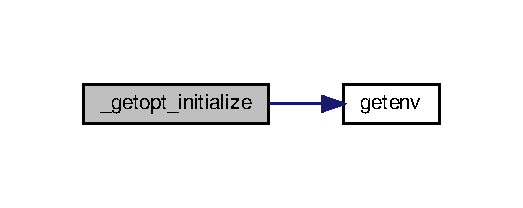
\includegraphics[width=251pt]{getopt_8c_a17475cbc1ffae0c12af2e0a3319d197f_cgraph}
\end{center}
\end{figure}
\mbox{\Hypertarget{getopt_8c_a0df92a0ae8fe1fd43268c738f548674f}\label{getopt_8c_a0df92a0ae8fe1fd43268c738f548674f}} 
\index{getopt.\+c@{getopt.\+c}!\+\_\+getopt\+\_\+internal@{\+\_\+getopt\+\_\+internal}}
\index{\+\_\+getopt\+\_\+internal@{\+\_\+getopt\+\_\+internal}!getopt.\+c@{getopt.\+c}}
\subsubsection{\texorpdfstring{\+\_\+getopt\+\_\+internal()}{\_getopt\_internal()}}
{\footnotesize\ttfamily int \+\_\+getopt\+\_\+internal (\begin{DoxyParamCaption}\item[{int}]{argc,  }\item[{char $\ast$\hyperlink{getopt_8c_a2c212835823e3c54a8ab6d95c652660e}{const} $\ast$}]{argv,  }\item[{\hyperlink{getopt_8c_a2c212835823e3c54a8ab6d95c652660e}{const} char $\ast$}]{optstring,  }\item[{\hyperlink{getopt_8c_a2c212835823e3c54a8ab6d95c652660e}{const} struct \hyperlink{structoption}{option} $\ast$}]{longopts,  }\item[{int $\ast$}]{longind,  }\item[{int}]{long\+\_\+only }\end{DoxyParamCaption})}

Here is the call graph for this function\+:
\nopagebreak
\begin{figure}[H]
\begin{center}
\leavevmode
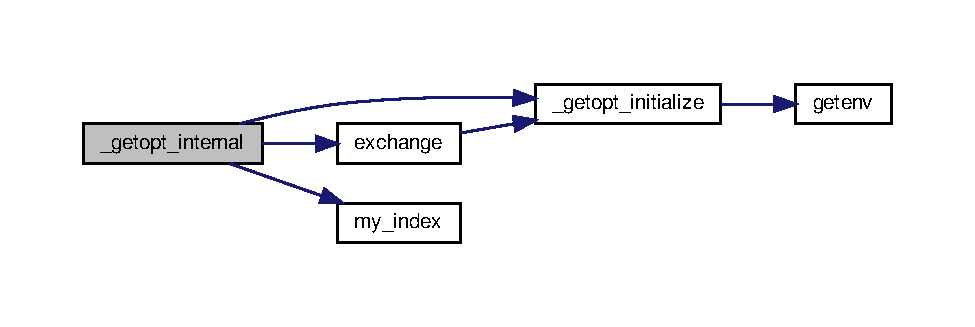
\includegraphics[width=350pt]{getopt_8c_a0df92a0ae8fe1fd43268c738f548674f_cgraph}
\end{center}
\end{figure}
\mbox{\Hypertarget{getopt_8c_a4621659dd6377e52ac50a0869625bb6e}\label{getopt_8c_a4621659dd6377e52ac50a0869625bb6e}} 
\index{getopt.\+c@{getopt.\+c}!exchange@{exchange}}
\index{exchange@{exchange}!getopt.\+c@{getopt.\+c}}
\subsubsection{\texorpdfstring{exchange()}{exchange()}}
{\footnotesize\ttfamily static void exchange (\begin{DoxyParamCaption}\item[{char $\ast$$\ast$}]{argv }\end{DoxyParamCaption})\hspace{0.3cm}{\ttfamily [static]}}

Here is the call graph for this function\+:
\nopagebreak
\begin{figure}[H]
\begin{center}
\leavevmode
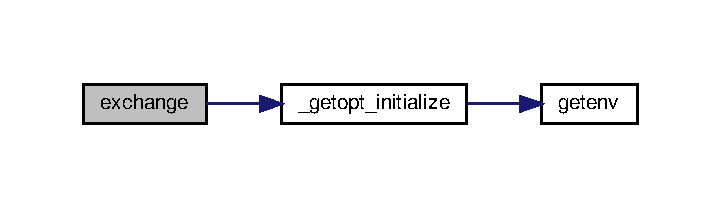
\includegraphics[width=346pt]{getopt_8c_a4621659dd6377e52ac50a0869625bb6e_cgraph}
\end{center}
\end{figure}
\mbox{\Hypertarget{getopt_8c_aee28fd8a0e40b6d958f7d20348e45368}\label{getopt_8c_aee28fd8a0e40b6d958f7d20348e45368}} 
\index{getopt.\+c@{getopt.\+c}!getenv@{getenv}}
\index{getenv@{getenv}!getopt.\+c@{getopt.\+c}}
\subsubsection{\texorpdfstring{getenv()}{getenv()}}
{\footnotesize\ttfamily char$\ast$ getenv (\begin{DoxyParamCaption}{ }\end{DoxyParamCaption})}

\mbox{\Hypertarget{getopt_8c_a1b2ada39ab92162c6ec9c67c8093fa2e}\label{getopt_8c_a1b2ada39ab92162c6ec9c67c8093fa2e}} 
\index{getopt.\+c@{getopt.\+c}!getopt@{getopt}}
\index{getopt@{getopt}!getopt.\+c@{getopt.\+c}}
\subsubsection{\texorpdfstring{getopt()}{getopt()}}
{\footnotesize\ttfamily int getopt (\begin{DoxyParamCaption}\item[{int}]{argc,  }\item[{char $\ast$\hyperlink{getopt_8c_a2c212835823e3c54a8ab6d95c652660e}{const} $\ast$}]{argv,  }\item[{\hyperlink{getopt_8c_a2c212835823e3c54a8ab6d95c652660e}{const} char $\ast$}]{optstring }\end{DoxyParamCaption})}

Here is the call graph for this function\+:
\nopagebreak
\begin{figure}[H]
\begin{center}
\leavevmode
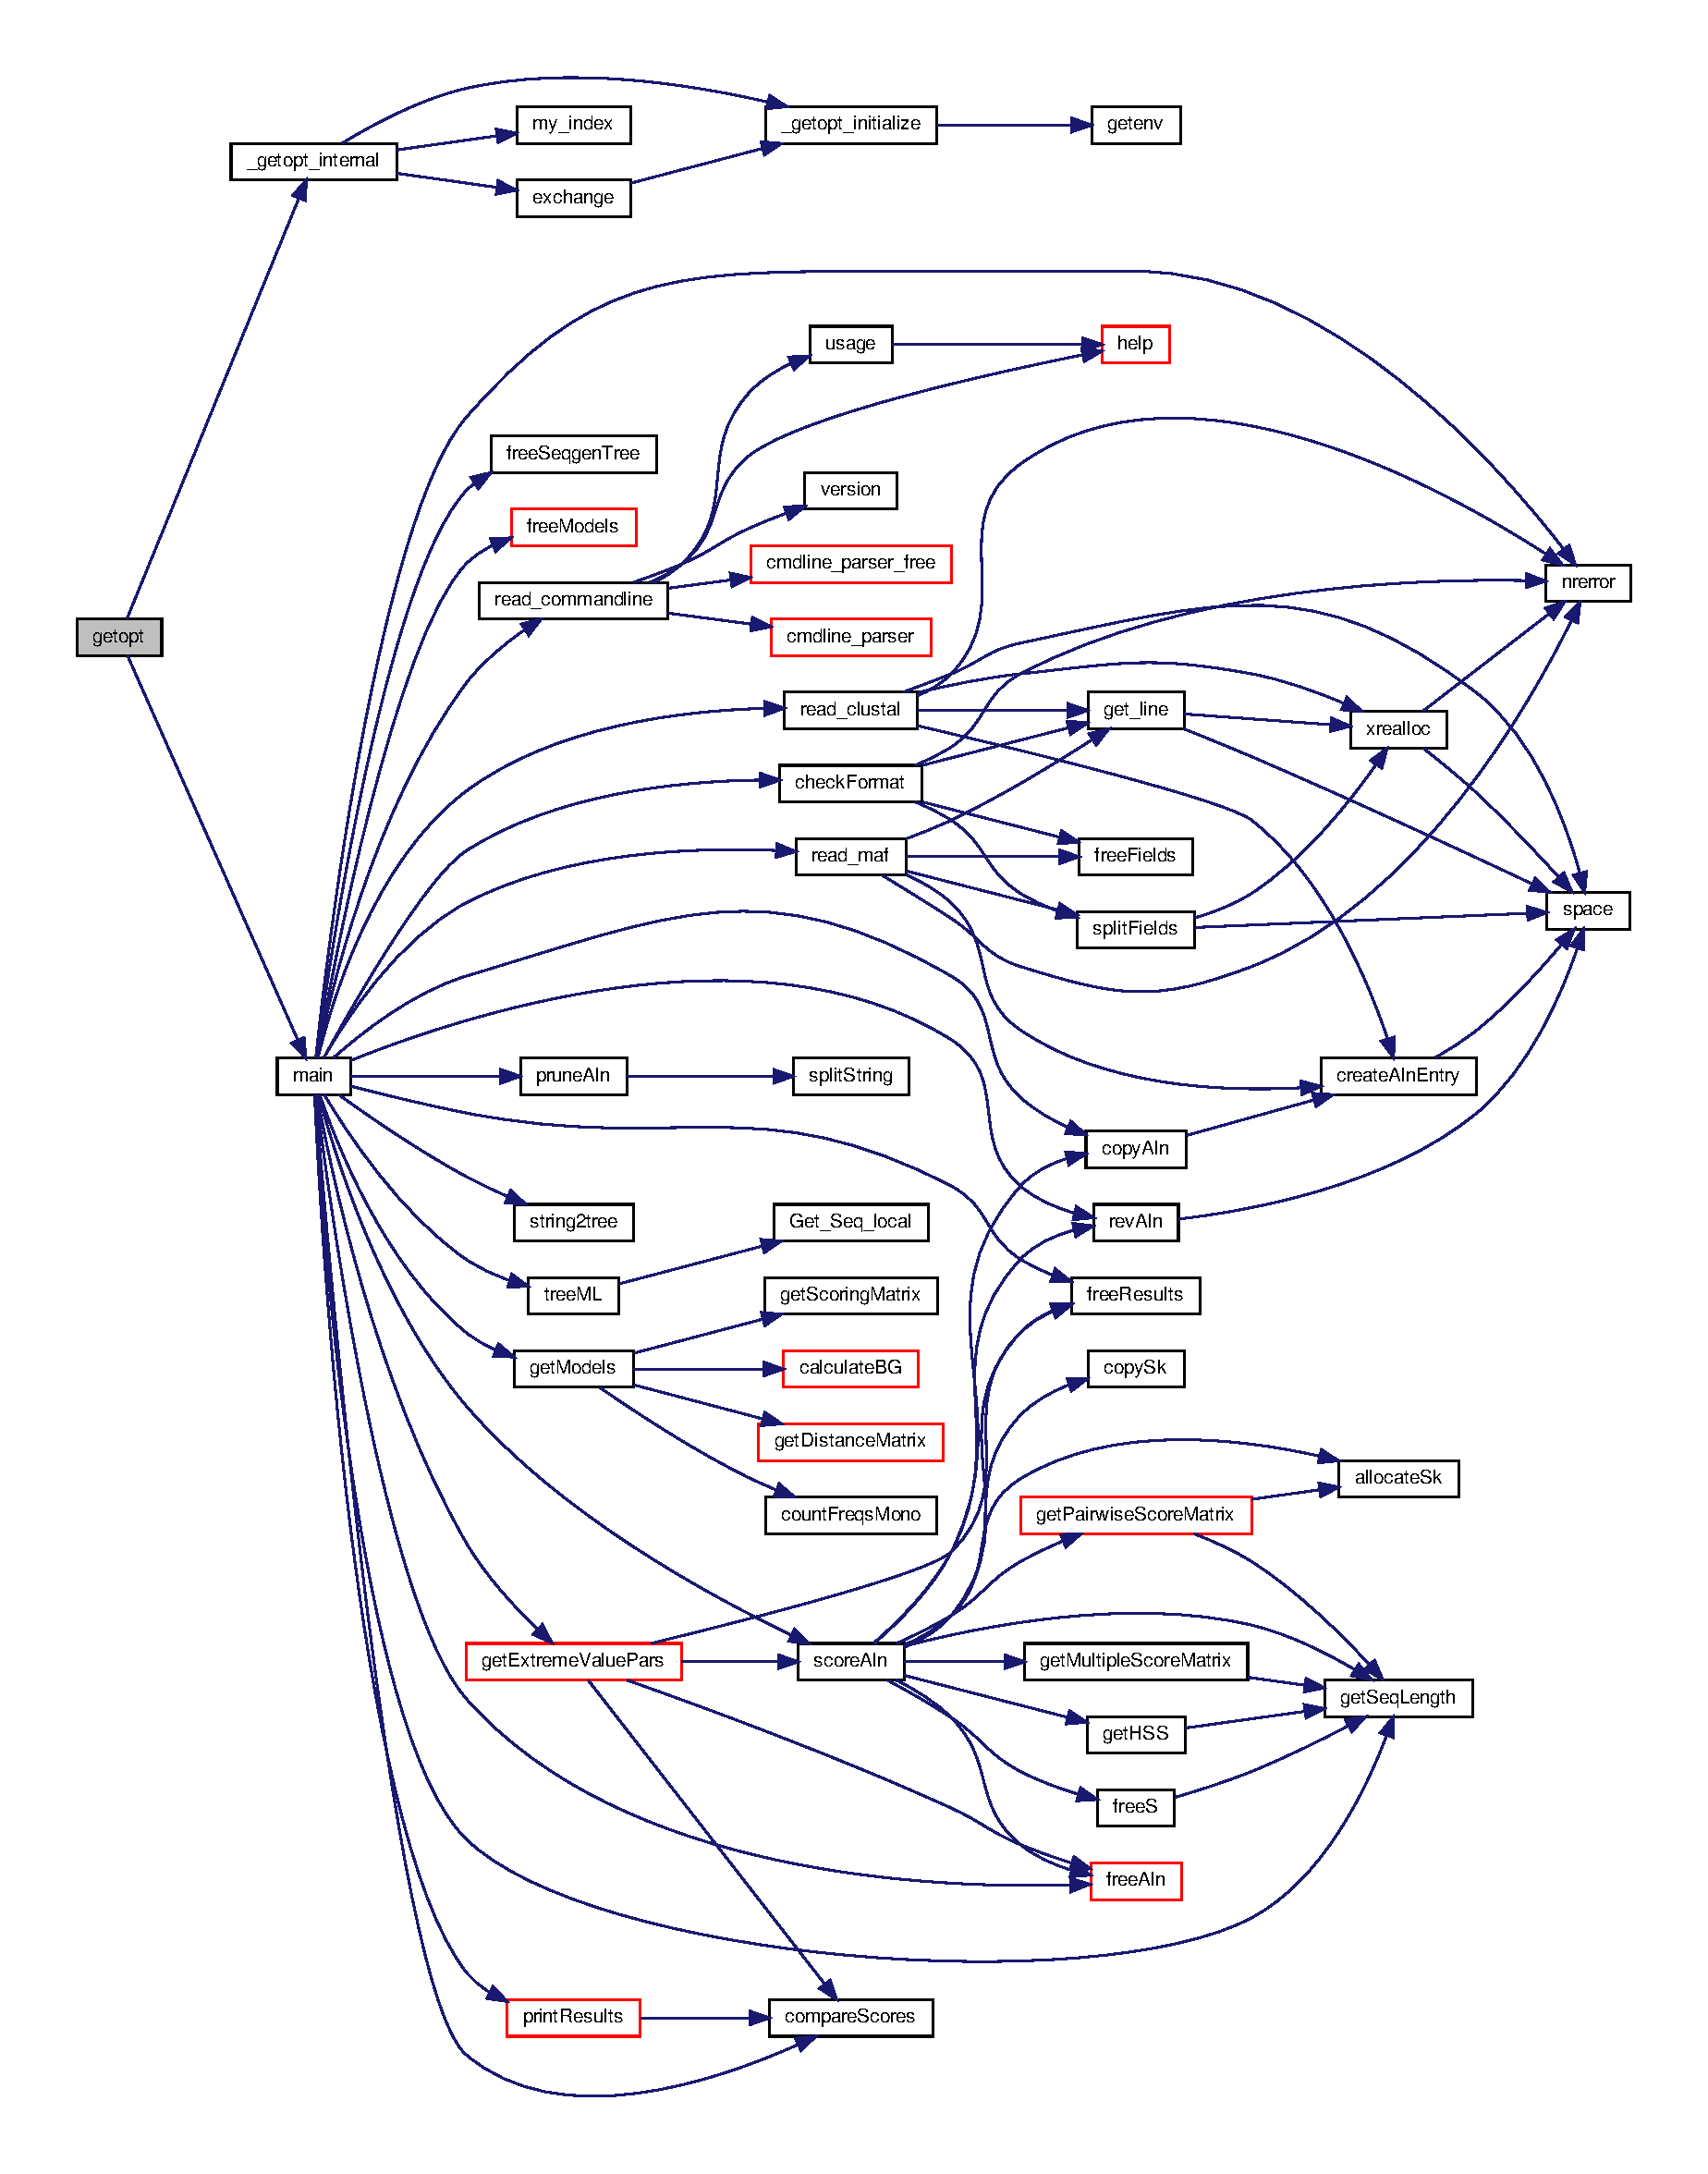
\includegraphics[width=350pt]{getopt_8c_a1b2ada39ab92162c6ec9c67c8093fa2e_cgraph}
\end{center}
\end{figure}
\mbox{\Hypertarget{getopt_8c_ae0ac978b7775f69496c0f127ffdada9d}\label{getopt_8c_ae0ac978b7775f69496c0f127ffdada9d}} 
\index{getopt.\+c@{getopt.\+c}!my\+\_\+index@{my\+\_\+index}}
\index{my\+\_\+index@{my\+\_\+index}!getopt.\+c@{getopt.\+c}}
\subsubsection{\texorpdfstring{my\+\_\+index()}{my\_index()}}
{\footnotesize\ttfamily static char$\ast$ my\+\_\+index (\begin{DoxyParamCaption}\item[{char $\ast$}]{str,  }\item[{int}]{chr }\end{DoxyParamCaption}) const\hspace{0.3cm}{\ttfamily [static]}}



\subsection{Variable Documentation}
\mbox{\Hypertarget{getopt_8c_a28286be757527aeb1db951b5da9aeec1}\label{getopt_8c_a28286be757527aeb1db951b5da9aeec1}} 
\index{getopt.\+c@{getopt.\+c}!\+\_\+\+\_\+getopt\+\_\+initialized@{\+\_\+\+\_\+getopt\+\_\+initialized}}
\index{\+\_\+\+\_\+getopt\+\_\+initialized@{\+\_\+\+\_\+getopt\+\_\+initialized}!getopt.\+c@{getopt.\+c}}
\subsubsection{\texorpdfstring{\+\_\+\+\_\+getopt\+\_\+initialized}{\_\_getopt\_initialized}}
{\footnotesize\ttfamily int \+\_\+\+\_\+getopt\+\_\+initialized}

\mbox{\Hypertarget{getopt_8c_a7b0f4f3bfbee147113f282427ce933ed}\label{getopt_8c_a7b0f4f3bfbee147113f282427ce933ed}} 
\index{getopt.\+c@{getopt.\+c}!first\+\_\+nonopt@{first\+\_\+nonopt}}
\index{first\+\_\+nonopt@{first\+\_\+nonopt}!getopt.\+c@{getopt.\+c}}
\subsubsection{\texorpdfstring{first\+\_\+nonopt}{first\_nonopt}}
{\footnotesize\ttfamily int first\+\_\+nonopt\hspace{0.3cm}{\ttfamily [static]}}

\mbox{\Hypertarget{getopt_8c_a580f2c2acf35dad51ca18b427212bf15}\label{getopt_8c_a580f2c2acf35dad51ca18b427212bf15}} 
\index{getopt.\+c@{getopt.\+c}!last\+\_\+nonopt@{last\+\_\+nonopt}}
\index{last\+\_\+nonopt@{last\+\_\+nonopt}!getopt.\+c@{getopt.\+c}}
\subsubsection{\texorpdfstring{last\+\_\+nonopt}{last\_nonopt}}
{\footnotesize\ttfamily int last\+\_\+nonopt\hspace{0.3cm}{\ttfamily [static]}}

\mbox{\Hypertarget{getopt_8c_a47a40a4c365dae45f94751ad32aab530}\label{getopt_8c_a47a40a4c365dae45f94751ad32aab530}} 
\index{getopt.\+c@{getopt.\+c}!nextchar@{nextchar}}
\index{nextchar@{nextchar}!getopt.\+c@{getopt.\+c}}
\subsubsection{\texorpdfstring{nextchar}{nextchar}}
{\footnotesize\ttfamily char$\ast$ nextchar\hspace{0.3cm}{\ttfamily [static]}}

\mbox{\Hypertarget{getopt_8c_adb50a0eab9fed92fc3bfc7dfa4f2c410}\label{getopt_8c_adb50a0eab9fed92fc3bfc7dfa4f2c410}} 
\index{getopt.\+c@{getopt.\+c}!optarg@{optarg}}
\index{optarg@{optarg}!getopt.\+c@{getopt.\+c}}
\subsubsection{\texorpdfstring{optarg}{optarg}}
{\footnotesize\ttfamily char$\ast$ optarg}

\mbox{\Hypertarget{getopt_8c_ae30f05ee1e2e5652f174a35c7875d25e}\label{getopt_8c_ae30f05ee1e2e5652f174a35c7875d25e}} 
\index{getopt.\+c@{getopt.\+c}!opterr@{opterr}}
\index{opterr@{opterr}!getopt.\+c@{getopt.\+c}}
\subsubsection{\texorpdfstring{opterr}{opterr}}
{\footnotesize\ttfamily int opterr = 1}

\mbox{\Hypertarget{getopt_8c_ad5e1c16213bbee2d5e8cc363309f418c}\label{getopt_8c_ad5e1c16213bbee2d5e8cc363309f418c}} 
\index{getopt.\+c@{getopt.\+c}!optind@{optind}}
\index{optind@{optind}!getopt.\+c@{getopt.\+c}}
\subsubsection{\texorpdfstring{optind}{optind}}
{\footnotesize\ttfamily int optind = 1}

\mbox{\Hypertarget{getopt_8c_a475b8db98445da73e5f62a1ef6324b95}\label{getopt_8c_a475b8db98445da73e5f62a1ef6324b95}} 
\index{getopt.\+c@{getopt.\+c}!optopt@{optopt}}
\index{optopt@{optopt}!getopt.\+c@{getopt.\+c}}
\subsubsection{\texorpdfstring{optopt}{optopt}}
{\footnotesize\ttfamily int optopt = \textquotesingle{}?\textquotesingle{}}

\mbox{\Hypertarget{getopt_8c_a67a84cf4dacaa8337be68345f8b9a8cc}\label{getopt_8c_a67a84cf4dacaa8337be68345f8b9a8cc}} 
\index{getopt.\+c@{getopt.\+c}!ordering@{ordering}}
\index{ordering@{ordering}!getopt.\+c@{getopt.\+c}}
\subsubsection{\texorpdfstring{ordering}{ordering}}
{\footnotesize\ttfamily enum \{ ... \}   ordering\hspace{0.3cm}{\ttfamily [static]}}

\mbox{\Hypertarget{getopt_8c_ad0ccb64bbd4defe7a57dbad2045ddd14}\label{getopt_8c_ad0ccb64bbd4defe7a57dbad2045ddd14}} 
\index{getopt.\+c@{getopt.\+c}!posixly\+\_\+correct@{posixly\+\_\+correct}}
\index{posixly\+\_\+correct@{posixly\+\_\+correct}!getopt.\+c@{getopt.\+c}}
\subsubsection{\texorpdfstring{posixly\+\_\+correct}{posixly\_correct}}
{\footnotesize\ttfamily char$\ast$ posixly\+\_\+correct\hspace{0.3cm}{\ttfamily [static]}}


\hypertarget{getopt_8h}{}\section{getopt.\+h File Reference}
\label{getopt_8h}\index{getopt.\+h@{getopt.\+h}}
This graph shows which files directly or indirectly include this file\+:
\nopagebreak
\begin{figure}[H]
\begin{center}
\leavevmode
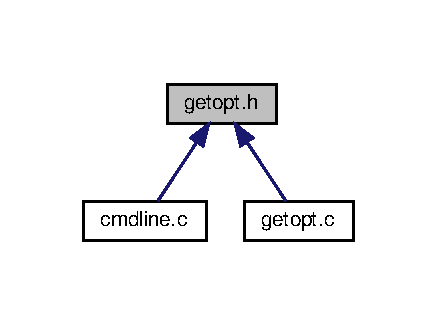
\includegraphics[width=210pt]{getopt_8h__dep__incl}
\end{center}
\end{figure}
\subsection*{Classes}
\begin{DoxyCompactItemize}
\item 
struct \hyperlink{structoption}{option}
\end{DoxyCompactItemize}
\subsection*{Macros}
\begin{DoxyCompactItemize}
\item 
\#define \hyperlink{getopt_8h_aaafc27a0389aa87797164b227566342d}{\+\_\+\+G\+E\+T\+O\+P\+T\+\_\+H}~1
\item 
\#define \hyperlink{getopt_8h_a3bc1d5f667b5b4ca4b4abb685dc874ce}{no\+\_\+argument}~0
\item 
\#define \hyperlink{getopt_8h_a6ece8d8dfa8378778f7290fdaba5b8bc}{required\+\_\+argument}~1
\item 
\#define \hyperlink{getopt_8h_acca06c0a947656bd8b395bf1084ffb72}{optional\+\_\+argument}~2
\end{DoxyCompactItemize}
\subsection*{Functions}
\begin{DoxyCompactItemize}
\item 
int \hyperlink{getopt_8h_a6c5b232cca42dab05f40b47f69715f8b}{getopt} ()
\item 
int \hyperlink{getopt_8h_a8616b8a74ae6c01a7ad95ad2876226ec}{getopt\+\_\+long} ()
\item 
int \hyperlink{getopt_8h_ac07930413317507d5c51c19b3ac6ed20}{getopt\+\_\+long\+\_\+only} ()
\item 
int \hyperlink{getopt_8h_a60428225710059ca135c6b2a8941855f}{\+\_\+getopt\+\_\+internal} ()
\end{DoxyCompactItemize}
\subsection*{Variables}
\begin{DoxyCompactItemize}
\item 
char $\ast$ \hyperlink{getopt_8h_adb50a0eab9fed92fc3bfc7dfa4f2c410}{optarg}
\item 
int \hyperlink{getopt_8h_ad5e1c16213bbee2d5e8cc363309f418c}{optind}
\item 
int \hyperlink{getopt_8h_ae30f05ee1e2e5652f174a35c7875d25e}{opterr}
\item 
int \hyperlink{getopt_8h_a475b8db98445da73e5f62a1ef6324b95}{optopt}
\end{DoxyCompactItemize}


\subsection{Macro Definition Documentation}
\mbox{\Hypertarget{getopt_8h_aaafc27a0389aa87797164b227566342d}\label{getopt_8h_aaafc27a0389aa87797164b227566342d}} 
\index{getopt.\+h@{getopt.\+h}!\+\_\+\+G\+E\+T\+O\+P\+T\+\_\+H@{\+\_\+\+G\+E\+T\+O\+P\+T\+\_\+H}}
\index{\+\_\+\+G\+E\+T\+O\+P\+T\+\_\+H@{\+\_\+\+G\+E\+T\+O\+P\+T\+\_\+H}!getopt.\+h@{getopt.\+h}}
\subsubsection{\texorpdfstring{\+\_\+\+G\+E\+T\+O\+P\+T\+\_\+H}{\_GETOPT\_H}}
{\footnotesize\ttfamily \#define \+\_\+\+G\+E\+T\+O\+P\+T\+\_\+H~1}

\mbox{\Hypertarget{getopt_8h_a3bc1d5f667b5b4ca4b4abb685dc874ce}\label{getopt_8h_a3bc1d5f667b5b4ca4b4abb685dc874ce}} 
\index{getopt.\+h@{getopt.\+h}!no\+\_\+argument@{no\+\_\+argument}}
\index{no\+\_\+argument@{no\+\_\+argument}!getopt.\+h@{getopt.\+h}}
\subsubsection{\texorpdfstring{no\+\_\+argument}{no\_argument}}
{\footnotesize\ttfamily \#define no\+\_\+argument~0}

\mbox{\Hypertarget{getopt_8h_acca06c0a947656bd8b395bf1084ffb72}\label{getopt_8h_acca06c0a947656bd8b395bf1084ffb72}} 
\index{getopt.\+h@{getopt.\+h}!optional\+\_\+argument@{optional\+\_\+argument}}
\index{optional\+\_\+argument@{optional\+\_\+argument}!getopt.\+h@{getopt.\+h}}
\subsubsection{\texorpdfstring{optional\+\_\+argument}{optional\_argument}}
{\footnotesize\ttfamily \#define optional\+\_\+argument~2}

\mbox{\Hypertarget{getopt_8h_a6ece8d8dfa8378778f7290fdaba5b8bc}\label{getopt_8h_a6ece8d8dfa8378778f7290fdaba5b8bc}} 
\index{getopt.\+h@{getopt.\+h}!required\+\_\+argument@{required\+\_\+argument}}
\index{required\+\_\+argument@{required\+\_\+argument}!getopt.\+h@{getopt.\+h}}
\subsubsection{\texorpdfstring{required\+\_\+argument}{required\_argument}}
{\footnotesize\ttfamily \#define required\+\_\+argument~1}



\subsection{Function Documentation}
\mbox{\Hypertarget{getopt_8h_a60428225710059ca135c6b2a8941855f}\label{getopt_8h_a60428225710059ca135c6b2a8941855f}} 
\index{getopt.\+h@{getopt.\+h}!\+\_\+getopt\+\_\+internal@{\+\_\+getopt\+\_\+internal}}
\index{\+\_\+getopt\+\_\+internal@{\+\_\+getopt\+\_\+internal}!getopt.\+h@{getopt.\+h}}
\subsubsection{\texorpdfstring{\+\_\+getopt\+\_\+internal()}{\_getopt\_internal()}}
{\footnotesize\ttfamily int \+\_\+getopt\+\_\+internal (\begin{DoxyParamCaption}{ }\end{DoxyParamCaption})}

\mbox{\Hypertarget{getopt_8h_a6c5b232cca42dab05f40b47f69715f8b}\label{getopt_8h_a6c5b232cca42dab05f40b47f69715f8b}} 
\index{getopt.\+h@{getopt.\+h}!getopt@{getopt}}
\index{getopt@{getopt}!getopt.\+h@{getopt.\+h}}
\subsubsection{\texorpdfstring{getopt()}{getopt()}}
{\footnotesize\ttfamily int getopt (\begin{DoxyParamCaption}{ }\end{DoxyParamCaption})}

\mbox{\Hypertarget{getopt_8h_a8616b8a74ae6c01a7ad95ad2876226ec}\label{getopt_8h_a8616b8a74ae6c01a7ad95ad2876226ec}} 
\index{getopt.\+h@{getopt.\+h}!getopt\+\_\+long@{getopt\+\_\+long}}
\index{getopt\+\_\+long@{getopt\+\_\+long}!getopt.\+h@{getopt.\+h}}
\subsubsection{\texorpdfstring{getopt\+\_\+long()}{getopt\_long()}}
{\footnotesize\ttfamily int getopt\+\_\+long (\begin{DoxyParamCaption}{ }\end{DoxyParamCaption})}

\mbox{\Hypertarget{getopt_8h_ac07930413317507d5c51c19b3ac6ed20}\label{getopt_8h_ac07930413317507d5c51c19b3ac6ed20}} 
\index{getopt.\+h@{getopt.\+h}!getopt\+\_\+long\+\_\+only@{getopt\+\_\+long\+\_\+only}}
\index{getopt\+\_\+long\+\_\+only@{getopt\+\_\+long\+\_\+only}!getopt.\+h@{getopt.\+h}}
\subsubsection{\texorpdfstring{getopt\+\_\+long\+\_\+only()}{getopt\_long\_only()}}
{\footnotesize\ttfamily int getopt\+\_\+long\+\_\+only (\begin{DoxyParamCaption}{ }\end{DoxyParamCaption})}



\subsection{Variable Documentation}
\mbox{\Hypertarget{getopt_8h_adb50a0eab9fed92fc3bfc7dfa4f2c410}\label{getopt_8h_adb50a0eab9fed92fc3bfc7dfa4f2c410}} 
\index{getopt.\+h@{getopt.\+h}!optarg@{optarg}}
\index{optarg@{optarg}!getopt.\+h@{getopt.\+h}}
\subsubsection{\texorpdfstring{optarg}{optarg}}
{\footnotesize\ttfamily char$\ast$ optarg}

\mbox{\Hypertarget{getopt_8h_ae30f05ee1e2e5652f174a35c7875d25e}\label{getopt_8h_ae30f05ee1e2e5652f174a35c7875d25e}} 
\index{getopt.\+h@{getopt.\+h}!opterr@{opterr}}
\index{opterr@{opterr}!getopt.\+h@{getopt.\+h}}
\subsubsection{\texorpdfstring{opterr}{opterr}}
{\footnotesize\ttfamily int opterr}

\mbox{\Hypertarget{getopt_8h_ad5e1c16213bbee2d5e8cc363309f418c}\label{getopt_8h_ad5e1c16213bbee2d5e8cc363309f418c}} 
\index{getopt.\+h@{getopt.\+h}!optind@{optind}}
\index{optind@{optind}!getopt.\+h@{getopt.\+h}}
\subsubsection{\texorpdfstring{optind}{optind}}
{\footnotesize\ttfamily int optind}

\mbox{\Hypertarget{getopt_8h_a475b8db98445da73e5f62a1ef6324b95}\label{getopt_8h_a475b8db98445da73e5f62a1ef6324b95}} 
\index{getopt.\+h@{getopt.\+h}!optopt@{optopt}}
\index{optopt@{optopt}!getopt.\+h@{getopt.\+h}}
\subsubsection{\texorpdfstring{optopt}{optopt}}
{\footnotesize\ttfamily int optopt}


\hypertarget{misc_8c}{}\section{misc.\+c File Reference}
\label{misc_8c}\index{misc.\+c@{misc.\+c}}
{\ttfamily \#include $<$string.\+h$>$}\newline
{\ttfamily \#include $<$stdio.\+h$>$}\newline
{\ttfamily \#include $<$stdlib.\+h$>$}\newline
{\ttfamily \#include $<$math.\+h$>$}\newline
{\ttfamily \#include $<$sys/stat.\+h$>$}\newline
{\ttfamily \#include $<$errno.\+h$>$}\newline
{\ttfamily \#include \char`\"{}R\+N\+Acode.\+h\char`\"{}}\newline
{\ttfamily \#include \char`\"{}misc.\+h\char`\"{}}\newline
{\ttfamily \#include \char`\"{}postscript.\+h\char`\"{}}\newline
Include dependency graph for misc.\+c\+:
\nopagebreak
\begin{figure}[H]
\begin{center}
\leavevmode
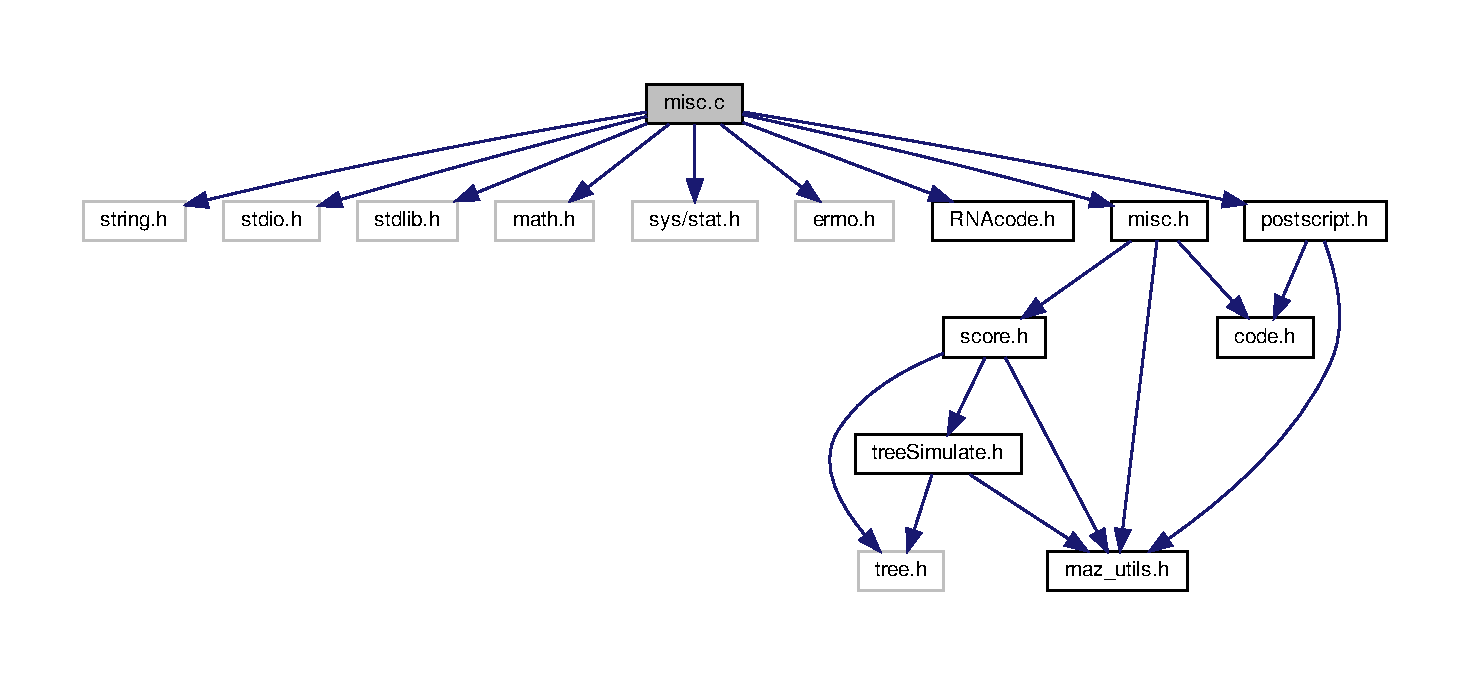
\includegraphics[width=350pt]{misc_8c__incl}
\end{center}
\end{figure}
\subsection*{Functions}
\begin{DoxyCompactItemize}
\item 
float $\ast$$\ast$$\ast$$\ast$ \hyperlink{misc_8c_ab8906f987e8caa1c304422e2105784db}{allocate\+Sk} (int N, int L)
\item 
void \hyperlink{misc_8c_a540d653adf9134e345a0be15556bef9f}{copy\+Sk} (float $\ast$$\ast$$\ast$$\ast$from, float $\ast$$\ast$$\ast$$\ast$to, int N, int L)
\item 
int \hyperlink{misc_8c_a3003bc209fbd623b0ebf8d55c3f76454}{compare\+Scores} (\hyperlink{getopt_8c_a2c212835823e3c54a8ab6d95c652660e}{const} void $\ast$a, \hyperlink{getopt_8c_a2c212835823e3c54a8ab6d95c652660e}{const} void $\ast$b)
\item 
int \hyperlink{misc_8c_a08c97f6ebbb296bfe2d0f74e7a3a8af8}{compare\+Location} (\hyperlink{getopt_8c_a2c212835823e3c54a8ab6d95c652660e}{const} void $\ast$a, \hyperlink{getopt_8c_a2c212835823e3c54a8ab6d95c652660e}{const} void $\ast$b)
\item 
void \hyperlink{misc_8c_a8eed68ed1197df02c8b9a49264efc717}{reintroduce\+Gaps} (\hyperlink{getopt_8c_a2c212835823e3c54a8ab6d95c652660e}{const} struct \hyperlink{structaln}{aln} $\ast$orig\+Aln\mbox{[}$\,$\mbox{]}, struct \hyperlink{structaln}{aln} $\ast$sampled\+Aln\mbox{[}$\,$\mbox{]})
\item 
void \hyperlink{misc_8c_a5753372a1a3c3974fc6be9a6030a67bf}{sort\+Aln} (\hyperlink{getopt_8c_a2c212835823e3c54a8ab6d95c652660e}{const} struct \hyperlink{structaln}{aln} $\ast$orig\+Aln\mbox{[}$\,$\mbox{]}, struct \hyperlink{structaln}{aln} $\ast$sampled\+Aln\mbox{[}$\,$\mbox{]})
\item 
void \hyperlink{misc_8c_a9fe543fe19ab3ff4ae9def519e1f0ac1}{get\+Block} (int i, \hyperlink{getopt_8c_a2c212835823e3c54a8ab6d95c652660e}{const} char $\ast$seq\+\_\+0, \hyperlink{getopt_8c_a2c212835823e3c54a8ab6d95c652660e}{const} char $\ast$seq\+\_\+k, \hyperlink{getopt_8c_a2c212835823e3c54a8ab6d95c652660e}{const} int $\ast$map\+\_\+0, \hyperlink{getopt_8c_a2c212835823e3c54a8ab6d95c652660e}{const} int $\ast$map\+\_\+k, char $\ast$block\+\_\+0, char $\ast$block\+\_\+k, int $\ast$z)
\item 
int \hyperlink{misc_8c_af49091737065e3ea21101edf17533dcf}{pos2col} (\hyperlink{getopt_8c_a2c212835823e3c54a8ab6d95c652660e}{const} char $\ast$seq, int pos)
\item 
int \hyperlink{misc_8c_a935b3901ff2b656c44257b4606ceab6c}{get\+Seq\+Length} (char $\ast$seq)
\item 
void \hyperlink{misc_8c_a71b140f8ccd1190776a6cc04f42f7b0d}{free\+Results} (\hyperlink{score_8h_a5b7f5df9506ff8c871dc49e4bf9f22af}{segment\+Stats} results\mbox{[}$\,$\mbox{]})
\item 
int \hyperlink{misc_8c_a62dbd6f5f78b8829c91c5e373b897f67}{h\+Dist} (int a1, int a2, int a3, int b1, int b2, int b3)
\item 
float \hyperlink{misc_8c_a29db63ab5182ac2f88eb37329c092126}{avg} (float $\ast$data, int N)
\item 
float \hyperlink{misc_8c_ac9b591bdb26f6a8b8ee56aee3e809c65}{stddev} (float $\ast$data, int N)
\item 
void \hyperlink{misc_8c_a0da1742a6a7f546827bee85fbdf53592}{copy\+Aln} (struct \hyperlink{structaln}{aln} $\ast$src\mbox{[}$\,$\mbox{]}, struct \hyperlink{structaln}{aln} $\ast$dest\mbox{[}$\,$\mbox{]})
\item 
void \hyperlink{misc_8c_a622e2235405d5fce48465d284271642c}{print\+Aln\+Clustal} (F\+I\+LE $\ast$out, \hyperlink{getopt_8c_a2c212835823e3c54a8ab6d95c652660e}{const} struct \hyperlink{structaln}{aln} $\ast$AS\mbox{[}$\,$\mbox{]})
\item 
void \hyperlink{misc_8c_a326b72f1de05ef655a3188af0af23aee}{print\+Results} (F\+I\+LE $\ast$\hyperlink{postscript_8c_ae581849c67336453bd5b81e6518019a9}{outfile}, int output\+Format, \hyperlink{getopt_8c_a2c212835823e3c54a8ab6d95c652660e}{const} struct \hyperlink{structaln}{aln} $\ast$input\+Aln\mbox{[}$\,$\mbox{]}, \hyperlink{score_8h_a5b7f5df9506ff8c871dc49e4bf9f22af}{segment\+Stats} results\mbox{[}$\,$\mbox{]})
\item 
int \hyperlink{misc_8c_a6017c986a43a1bba1569a8efb1b3aedb}{extend\+Region} (\hyperlink{getopt_8c_a2c212835823e3c54a8ab6d95c652660e}{const} struct \hyperlink{structaln}{aln} $\ast$alignment\mbox{[}$\,$\mbox{]}, int pos, int direction)
\end{DoxyCompactItemize}
\subsection*{Variables}
\begin{DoxyCompactItemize}
\item 
\hyperlink{RNAcode_8h_ac21aeabbefffddb27496994611a09dcd}{parameters} \hyperlink{misc_8c_a8dea3b88a171ed8de9f8f98079e7561a}{pars}
\item 
long int \hyperlink{misc_8c_a8c5872fcd4604b525d509ffd6afc5631}{hit\+Counter}
\end{DoxyCompactItemize}


\subsection{Function Documentation}
\mbox{\Hypertarget{misc_8c_ab8906f987e8caa1c304422e2105784db}\label{misc_8c_ab8906f987e8caa1c304422e2105784db}} 
\index{misc.\+c@{misc.\+c}!allocate\+Sk@{allocate\+Sk}}
\index{allocate\+Sk@{allocate\+Sk}!misc.\+c@{misc.\+c}}
\subsubsection{\texorpdfstring{allocate\+Sk()}{allocateSk()}}
{\footnotesize\ttfamily float$\ast$$\ast$$\ast$$\ast$ allocate\+Sk (\begin{DoxyParamCaption}\item[{int}]{N,  }\item[{int}]{L }\end{DoxyParamCaption})}

\mbox{\Hypertarget{misc_8c_a29db63ab5182ac2f88eb37329c092126}\label{misc_8c_a29db63ab5182ac2f88eb37329c092126}} 
\index{misc.\+c@{misc.\+c}!avg@{avg}}
\index{avg@{avg}!misc.\+c@{misc.\+c}}
\subsubsection{\texorpdfstring{avg()}{avg()}}
{\footnotesize\ttfamily float avg (\begin{DoxyParamCaption}\item[{float $\ast$}]{data,  }\item[{int}]{N }\end{DoxyParamCaption})}

\mbox{\Hypertarget{misc_8c_a08c97f6ebbb296bfe2d0f74e7a3a8af8}\label{misc_8c_a08c97f6ebbb296bfe2d0f74e7a3a8af8}} 
\index{misc.\+c@{misc.\+c}!compare\+Location@{compare\+Location}}
\index{compare\+Location@{compare\+Location}!misc.\+c@{misc.\+c}}
\subsubsection{\texorpdfstring{compare\+Location()}{compareLocation()}}
{\footnotesize\ttfamily int compare\+Location (\begin{DoxyParamCaption}\item[{\hyperlink{getopt_8c_a2c212835823e3c54a8ab6d95c652660e}{const} void $\ast$}]{a,  }\item[{\hyperlink{getopt_8c_a2c212835823e3c54a8ab6d95c652660e}{const} void $\ast$}]{b }\end{DoxyParamCaption})}

\mbox{\Hypertarget{misc_8c_a3003bc209fbd623b0ebf8d55c3f76454}\label{misc_8c_a3003bc209fbd623b0ebf8d55c3f76454}} 
\index{misc.\+c@{misc.\+c}!compare\+Scores@{compare\+Scores}}
\index{compare\+Scores@{compare\+Scores}!misc.\+c@{misc.\+c}}
\subsubsection{\texorpdfstring{compare\+Scores()}{compareScores()}}
{\footnotesize\ttfamily int compare\+Scores (\begin{DoxyParamCaption}\item[{\hyperlink{getopt_8c_a2c212835823e3c54a8ab6d95c652660e}{const} void $\ast$}]{a,  }\item[{\hyperlink{getopt_8c_a2c212835823e3c54a8ab6d95c652660e}{const} void $\ast$}]{b }\end{DoxyParamCaption})}

\mbox{\Hypertarget{misc_8c_a0da1742a6a7f546827bee85fbdf53592}\label{misc_8c_a0da1742a6a7f546827bee85fbdf53592}} 
\index{misc.\+c@{misc.\+c}!copy\+Aln@{copy\+Aln}}
\index{copy\+Aln@{copy\+Aln}!misc.\+c@{misc.\+c}}
\subsubsection{\texorpdfstring{copy\+Aln()}{copyAln()}}
{\footnotesize\ttfamily void copy\+Aln (\begin{DoxyParamCaption}\item[{struct \hyperlink{structaln}{aln} $\ast$}]{src\mbox{[}$\,$\mbox{]},  }\item[{struct \hyperlink{structaln}{aln} $\ast$}]{dest\mbox{[}$\,$\mbox{]} }\end{DoxyParamCaption})}

Here is the call graph for this function\+:
\nopagebreak
\begin{figure}[H]
\begin{center}
\leavevmode
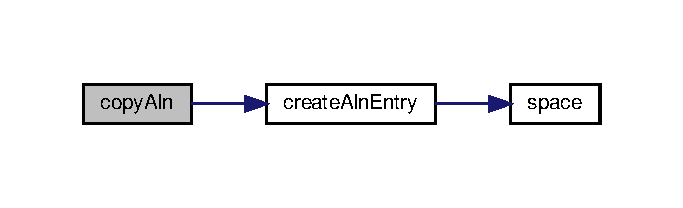
\includegraphics[width=328pt]{misc_8c_a0da1742a6a7f546827bee85fbdf53592_cgraph}
\end{center}
\end{figure}
\mbox{\Hypertarget{misc_8c_a540d653adf9134e345a0be15556bef9f}\label{misc_8c_a540d653adf9134e345a0be15556bef9f}} 
\index{misc.\+c@{misc.\+c}!copy\+Sk@{copy\+Sk}}
\index{copy\+Sk@{copy\+Sk}!misc.\+c@{misc.\+c}}
\subsubsection{\texorpdfstring{copy\+Sk()}{copySk()}}
{\footnotesize\ttfamily void copy\+Sk (\begin{DoxyParamCaption}\item[{float $\ast$$\ast$$\ast$$\ast$}]{from,  }\item[{float $\ast$$\ast$$\ast$$\ast$}]{to,  }\item[{int}]{N,  }\item[{int}]{L }\end{DoxyParamCaption})}

\mbox{\Hypertarget{misc_8c_a6017c986a43a1bba1569a8efb1b3aedb}\label{misc_8c_a6017c986a43a1bba1569a8efb1b3aedb}} 
\index{misc.\+c@{misc.\+c}!extend\+Region@{extend\+Region}}
\index{extend\+Region@{extend\+Region}!misc.\+c@{misc.\+c}}
\subsubsection{\texorpdfstring{extend\+Region()}{extendRegion()}}
{\footnotesize\ttfamily int extend\+Region (\begin{DoxyParamCaption}\item[{\hyperlink{getopt_8c_a2c212835823e3c54a8ab6d95c652660e}{const} struct \hyperlink{structaln}{aln} $\ast$}]{alignment\mbox{[}$\,$\mbox{]},  }\item[{int}]{pos,  }\item[{int}]{direction }\end{DoxyParamCaption})}

Here is the call graph for this function\+:
\nopagebreak
\begin{figure}[H]
\begin{center}
\leavevmode
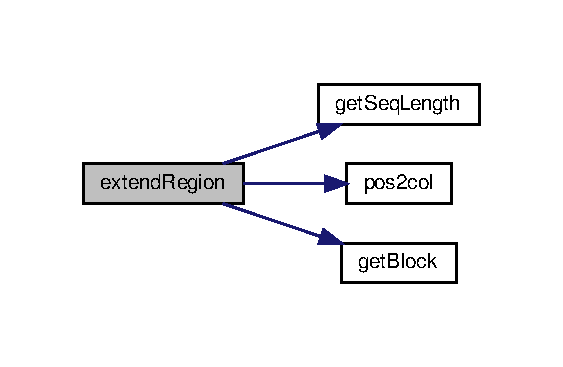
\includegraphics[width=270pt]{misc_8c_a6017c986a43a1bba1569a8efb1b3aedb_cgraph}
\end{center}
\end{figure}
\mbox{\Hypertarget{misc_8c_a71b140f8ccd1190776a6cc04f42f7b0d}\label{misc_8c_a71b140f8ccd1190776a6cc04f42f7b0d}} 
\index{misc.\+c@{misc.\+c}!free\+Results@{free\+Results}}
\index{free\+Results@{free\+Results}!misc.\+c@{misc.\+c}}
\subsubsection{\texorpdfstring{free\+Results()}{freeResults()}}
{\footnotesize\ttfamily void free\+Results (\begin{DoxyParamCaption}\item[{\hyperlink{score_8h_a5b7f5df9506ff8c871dc49e4bf9f22af}{segment\+Stats}}]{results\mbox{[}$\,$\mbox{]} }\end{DoxyParamCaption})}

\mbox{\Hypertarget{misc_8c_a9fe543fe19ab3ff4ae9def519e1f0ac1}\label{misc_8c_a9fe543fe19ab3ff4ae9def519e1f0ac1}} 
\index{misc.\+c@{misc.\+c}!get\+Block@{get\+Block}}
\index{get\+Block@{get\+Block}!misc.\+c@{misc.\+c}}
\subsubsection{\texorpdfstring{get\+Block()}{getBlock()}}
{\footnotesize\ttfamily void get\+Block (\begin{DoxyParamCaption}\item[{int}]{i,  }\item[{\hyperlink{getopt_8c_a2c212835823e3c54a8ab6d95c652660e}{const} char $\ast$}]{seq\+\_\+0,  }\item[{\hyperlink{getopt_8c_a2c212835823e3c54a8ab6d95c652660e}{const} char $\ast$}]{seq\+\_\+k,  }\item[{\hyperlink{getopt_8c_a2c212835823e3c54a8ab6d95c652660e}{const} int $\ast$}]{map\+\_\+0,  }\item[{\hyperlink{getopt_8c_a2c212835823e3c54a8ab6d95c652660e}{const} int $\ast$}]{map\+\_\+k,  }\item[{char $\ast$}]{block\+\_\+0,  }\item[{char $\ast$}]{block\+\_\+k,  }\item[{int $\ast$}]{z }\end{DoxyParamCaption})}

\mbox{\Hypertarget{misc_8c_a935b3901ff2b656c44257b4606ceab6c}\label{misc_8c_a935b3901ff2b656c44257b4606ceab6c}} 
\index{misc.\+c@{misc.\+c}!get\+Seq\+Length@{get\+Seq\+Length}}
\index{get\+Seq\+Length@{get\+Seq\+Length}!misc.\+c@{misc.\+c}}
\subsubsection{\texorpdfstring{get\+Seq\+Length()}{getSeqLength()}}
{\footnotesize\ttfamily int get\+Seq\+Length (\begin{DoxyParamCaption}\item[{char $\ast$}]{seq }\end{DoxyParamCaption})}

\mbox{\Hypertarget{misc_8c_a62dbd6f5f78b8829c91c5e373b897f67}\label{misc_8c_a62dbd6f5f78b8829c91c5e373b897f67}} 
\index{misc.\+c@{misc.\+c}!h\+Dist@{h\+Dist}}
\index{h\+Dist@{h\+Dist}!misc.\+c@{misc.\+c}}
\subsubsection{\texorpdfstring{h\+Dist()}{hDist()}}
{\footnotesize\ttfamily int h\+Dist (\begin{DoxyParamCaption}\item[{int}]{a1,  }\item[{int}]{a2,  }\item[{int}]{a3,  }\item[{int}]{b1,  }\item[{int}]{b2,  }\item[{int}]{b3 }\end{DoxyParamCaption})}

\mbox{\Hypertarget{misc_8c_af49091737065e3ea21101edf17533dcf}\label{misc_8c_af49091737065e3ea21101edf17533dcf}} 
\index{misc.\+c@{misc.\+c}!pos2col@{pos2col}}
\index{pos2col@{pos2col}!misc.\+c@{misc.\+c}}
\subsubsection{\texorpdfstring{pos2col()}{pos2col()}}
{\footnotesize\ttfamily int pos2col (\begin{DoxyParamCaption}\item[{\hyperlink{getopt_8c_a2c212835823e3c54a8ab6d95c652660e}{const} char $\ast$}]{seq,  }\item[{int}]{pos }\end{DoxyParamCaption})}

\mbox{\Hypertarget{misc_8c_a622e2235405d5fce48465d284271642c}\label{misc_8c_a622e2235405d5fce48465d284271642c}} 
\index{misc.\+c@{misc.\+c}!print\+Aln\+Clustal@{print\+Aln\+Clustal}}
\index{print\+Aln\+Clustal@{print\+Aln\+Clustal}!misc.\+c@{misc.\+c}}
\subsubsection{\texorpdfstring{print\+Aln\+Clustal()}{printAlnClustal()}}
{\footnotesize\ttfamily void print\+Aln\+Clustal (\begin{DoxyParamCaption}\item[{F\+I\+LE $\ast$}]{out,  }\item[{\hyperlink{getopt_8c_a2c212835823e3c54a8ab6d95c652660e}{const} struct \hyperlink{structaln}{aln} $\ast$}]{AS\mbox{[}$\,$\mbox{]} }\end{DoxyParamCaption})}

\mbox{\Hypertarget{misc_8c_a326b72f1de05ef655a3188af0af23aee}\label{misc_8c_a326b72f1de05ef655a3188af0af23aee}} 
\index{misc.\+c@{misc.\+c}!print\+Results@{print\+Results}}
\index{print\+Results@{print\+Results}!misc.\+c@{misc.\+c}}
\subsubsection{\texorpdfstring{print\+Results()}{printResults()}}
{\footnotesize\ttfamily void print\+Results (\begin{DoxyParamCaption}\item[{F\+I\+LE $\ast$}]{outfile,  }\item[{int}]{output\+Format,  }\item[{\hyperlink{getopt_8c_a2c212835823e3c54a8ab6d95c652660e}{const} struct \hyperlink{structaln}{aln} $\ast$}]{input\+Aln\mbox{[}$\,$\mbox{]},  }\item[{\hyperlink{score_8h_a5b7f5df9506ff8c871dc49e4bf9f22af}{segment\+Stats}}]{results\mbox{[}$\,$\mbox{]} }\end{DoxyParamCaption})}

Here is the call graph for this function\+:
\nopagebreak
\begin{figure}[H]
\begin{center}
\leavevmode
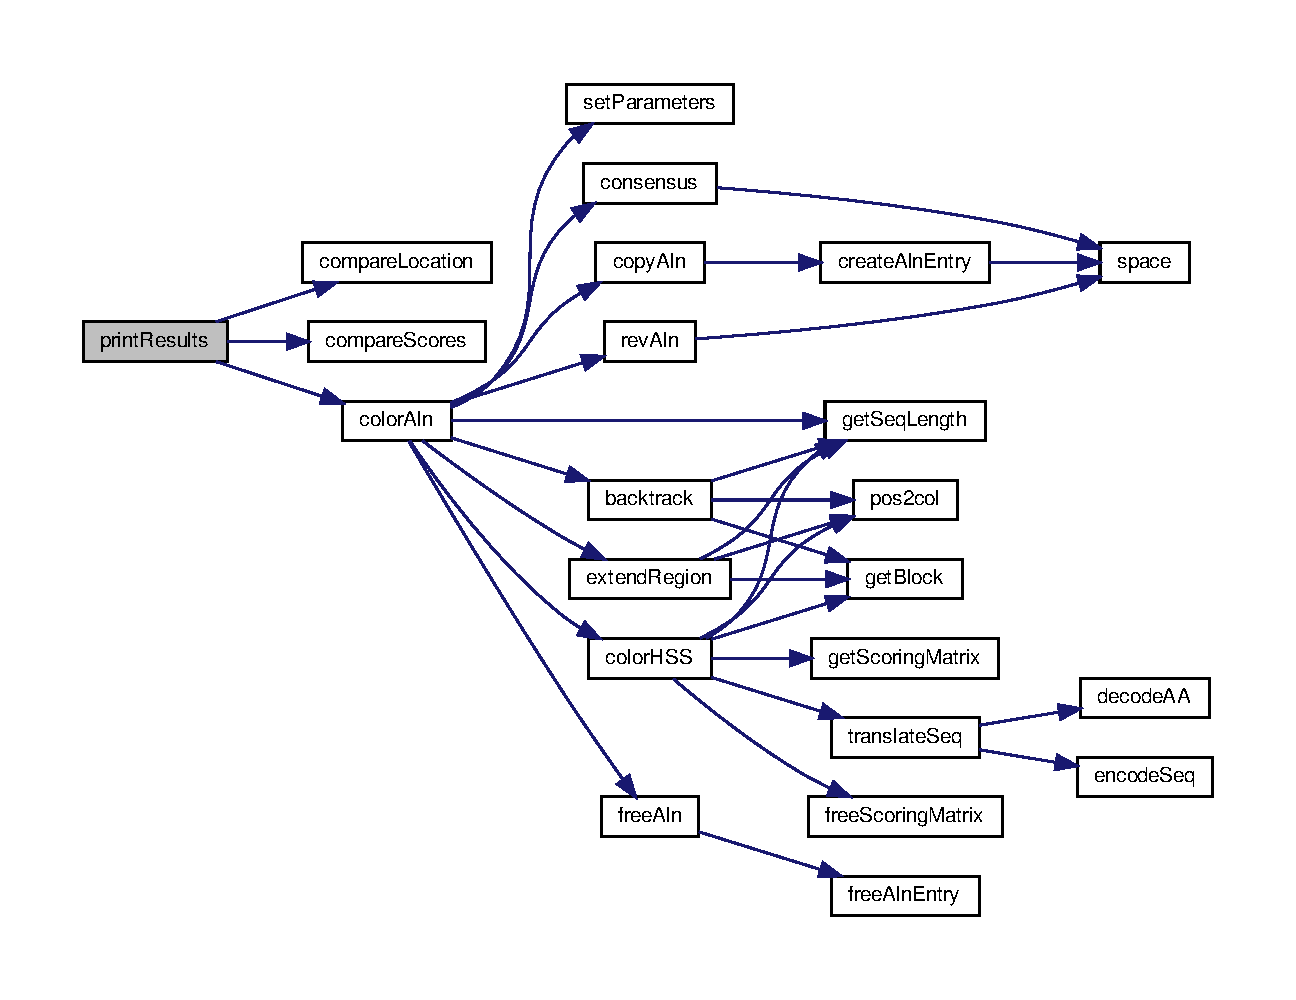
\includegraphics[width=350pt]{misc_8c_a326b72f1de05ef655a3188af0af23aee_cgraph}
\end{center}
\end{figure}
\mbox{\Hypertarget{misc_8c_a8eed68ed1197df02c8b9a49264efc717}\label{misc_8c_a8eed68ed1197df02c8b9a49264efc717}} 
\index{misc.\+c@{misc.\+c}!reintroduce\+Gaps@{reintroduce\+Gaps}}
\index{reintroduce\+Gaps@{reintroduce\+Gaps}!misc.\+c@{misc.\+c}}
\subsubsection{\texorpdfstring{reintroduce\+Gaps()}{reintroduceGaps()}}
{\footnotesize\ttfamily void reintroduce\+Gaps (\begin{DoxyParamCaption}\item[{\hyperlink{getopt_8c_a2c212835823e3c54a8ab6d95c652660e}{const} struct \hyperlink{structaln}{aln} $\ast$}]{orig\+Aln\mbox{[}$\,$\mbox{]},  }\item[{struct \hyperlink{structaln}{aln} $\ast$}]{sampled\+Aln\mbox{[}$\,$\mbox{]} }\end{DoxyParamCaption})}

\mbox{\Hypertarget{misc_8c_a5753372a1a3c3974fc6be9a6030a67bf}\label{misc_8c_a5753372a1a3c3974fc6be9a6030a67bf}} 
\index{misc.\+c@{misc.\+c}!sort\+Aln@{sort\+Aln}}
\index{sort\+Aln@{sort\+Aln}!misc.\+c@{misc.\+c}}
\subsubsection{\texorpdfstring{sort\+Aln()}{sortAln()}}
{\footnotesize\ttfamily void sort\+Aln (\begin{DoxyParamCaption}\item[{\hyperlink{getopt_8c_a2c212835823e3c54a8ab6d95c652660e}{const} struct \hyperlink{structaln}{aln} $\ast$}]{orig\+Aln\mbox{[}$\,$\mbox{]},  }\item[{struct \hyperlink{structaln}{aln} $\ast$}]{sampled\+Aln\mbox{[}$\,$\mbox{]} }\end{DoxyParamCaption})}

\mbox{\Hypertarget{misc_8c_ac9b591bdb26f6a8b8ee56aee3e809c65}\label{misc_8c_ac9b591bdb26f6a8b8ee56aee3e809c65}} 
\index{misc.\+c@{misc.\+c}!stddev@{stddev}}
\index{stddev@{stddev}!misc.\+c@{misc.\+c}}
\subsubsection{\texorpdfstring{stddev()}{stddev()}}
{\footnotesize\ttfamily float stddev (\begin{DoxyParamCaption}\item[{float $\ast$}]{data,  }\item[{int}]{N }\end{DoxyParamCaption})}



\subsection{Variable Documentation}
\mbox{\Hypertarget{misc_8c_a8c5872fcd4604b525d509ffd6afc5631}\label{misc_8c_a8c5872fcd4604b525d509ffd6afc5631}} 
\index{misc.\+c@{misc.\+c}!hit\+Counter@{hit\+Counter}}
\index{hit\+Counter@{hit\+Counter}!misc.\+c@{misc.\+c}}
\subsubsection{\texorpdfstring{hit\+Counter}{hitCounter}}
{\footnotesize\ttfamily long int hit\+Counter}

\mbox{\Hypertarget{misc_8c_a8dea3b88a171ed8de9f8f98079e7561a}\label{misc_8c_a8dea3b88a171ed8de9f8f98079e7561a}} 
\index{misc.\+c@{misc.\+c}!pars@{pars}}
\index{pars@{pars}!misc.\+c@{misc.\+c}}
\subsubsection{\texorpdfstring{pars}{pars}}
{\footnotesize\ttfamily \hyperlink{RNAcode_8h_ac21aeabbefffddb27496994611a09dcd}{parameters} pars}


\hypertarget{misc_8h}{}\section{misc.\+h File Reference}
\label{misc_8h}\index{misc.\+h@{misc.\+h}}
{\ttfamily \#include \char`\"{}score.\+h\char`\"{}}\newline
{\ttfamily \#include \char`\"{}code.\+h\char`\"{}}\newline
{\ttfamily \#include \char`\"{}rnaz\+\_\+utils.\+h\char`\"{}}\newline
Include dependency graph for misc.\+h\+:
\nopagebreak
\begin{figure}[H]
\begin{center}
\leavevmode
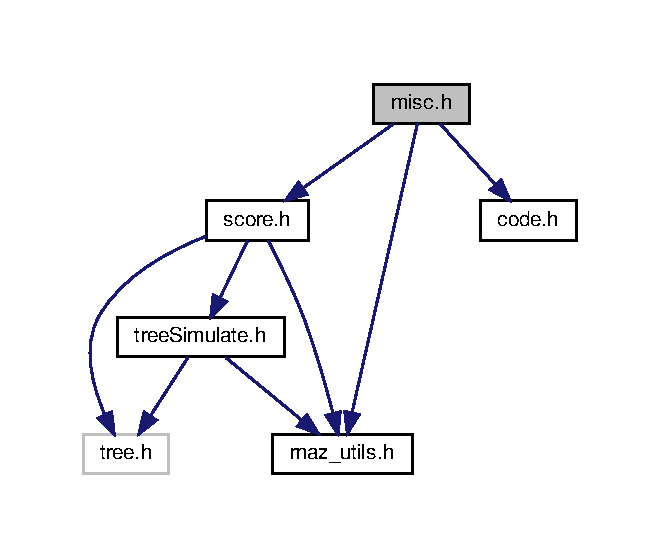
\includegraphics[width=317pt]{misc_8h__incl}
\end{center}
\end{figure}
This graph shows which files directly or indirectly include this file\+:
\nopagebreak
\begin{figure}[H]
\begin{center}
\leavevmode
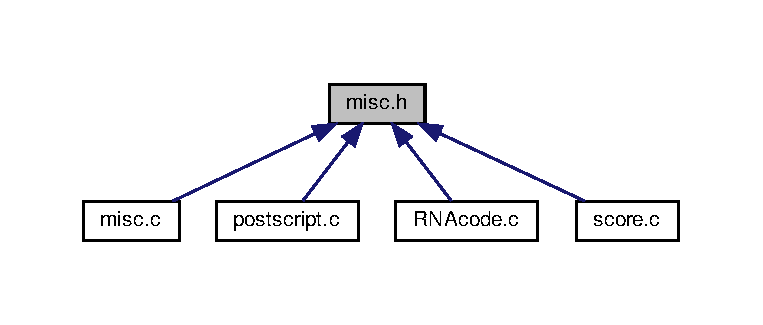
\includegraphics[width=350pt]{misc_8h__dep__incl}
\end{center}
\end{figure}
\subsection*{Functions}
\begin{DoxyCompactItemize}
\item 
float $\ast$$\ast$$\ast$$\ast$ \hyperlink{misc_8h_ab8906f987e8caa1c304422e2105784db}{allocate\+Sk} (int N, int L)
\item 
void \hyperlink{misc_8h_a540d653adf9134e345a0be15556bef9f}{copy\+Sk} (float $\ast$$\ast$$\ast$$\ast$from, float $\ast$$\ast$$\ast$$\ast$to, int N, int L)
\item 
int \hyperlink{misc_8h_a3003bc209fbd623b0ebf8d55c3f76454}{compare\+Scores} (\hyperlink{getopt_8c_a2c212835823e3c54a8ab6d95c652660e}{const} void $\ast$a, \hyperlink{getopt_8c_a2c212835823e3c54a8ab6d95c652660e}{const} void $\ast$b)
\item 
void \hyperlink{misc_8h_a8eed68ed1197df02c8b9a49264efc717}{reintroduce\+Gaps} (\hyperlink{getopt_8c_a2c212835823e3c54a8ab6d95c652660e}{const} struct \hyperlink{structaln}{aln} $\ast$orig\+Aln\mbox{[}$\,$\mbox{]}, struct \hyperlink{structaln}{aln} $\ast$sampled\+Aln\mbox{[}$\,$\mbox{]})
\item 
void \hyperlink{misc_8h_a5753372a1a3c3974fc6be9a6030a67bf}{sort\+Aln} (\hyperlink{getopt_8c_a2c212835823e3c54a8ab6d95c652660e}{const} struct \hyperlink{structaln}{aln} $\ast$orig\+Aln\mbox{[}$\,$\mbox{]}, struct \hyperlink{structaln}{aln} $\ast$sampled\+Aln\mbox{[}$\,$\mbox{]})
\item 
void \hyperlink{misc_8h_a71b140f8ccd1190776a6cc04f42f7b0d}{free\+Results} (\hyperlink{score_8h_a5b7f5df9506ff8c871dc49e4bf9f22af}{segment\+Stats} results\mbox{[}$\,$\mbox{]})
\item 
void \hyperlink{misc_8h_a9fe543fe19ab3ff4ae9def519e1f0ac1}{get\+Block} (int i, \hyperlink{getopt_8c_a2c212835823e3c54a8ab6d95c652660e}{const} char $\ast$seq\+\_\+0, \hyperlink{getopt_8c_a2c212835823e3c54a8ab6d95c652660e}{const} char $\ast$seq\+\_\+k, \hyperlink{getopt_8c_a2c212835823e3c54a8ab6d95c652660e}{const} int $\ast$map\+\_\+0, \hyperlink{getopt_8c_a2c212835823e3c54a8ab6d95c652660e}{const} int $\ast$map\+\_\+k, char $\ast$block\+\_\+0, char $\ast$block\+\_\+k, int $\ast$z)
\item 
int \hyperlink{misc_8h_af49091737065e3ea21101edf17533dcf}{pos2col} (\hyperlink{getopt_8c_a2c212835823e3c54a8ab6d95c652660e}{const} char $\ast$seq, int pos)
\item 
int \hyperlink{misc_8h_a935b3901ff2b656c44257b4606ceab6c}{get\+Seq\+Length} (char $\ast$seq)
\item 
int \hyperlink{misc_8h_a62dbd6f5f78b8829c91c5e373b897f67}{h\+Dist} (int a1, int a2, int a3, int b1, int b2, int b3)
\item 
float \hyperlink{misc_8h_a29db63ab5182ac2f88eb37329c092126}{avg} (float $\ast$data, int N)
\item 
float \hyperlink{misc_8h_ac9b591bdb26f6a8b8ee56aee3e809c65}{stddev} (float $\ast$data, int N)
\item 
float \hyperlink{misc_8h_af625860d4b3644771a9b58a316518d00}{gaussian} (\hyperlink{getopt_8c_a2c212835823e3c54a8ab6d95c652660e}{const} float sigma)
\item 
void \hyperlink{misc_8h_a0da1742a6a7f546827bee85fbdf53592}{copy\+Aln} (struct \hyperlink{structaln}{aln} $\ast$src\mbox{[}$\,$\mbox{]}, struct \hyperlink{structaln}{aln} $\ast$dest\mbox{[}$\,$\mbox{]})
\item 
void \hyperlink{misc_8h_a622e2235405d5fce48465d284271642c}{print\+Aln\+Clustal} (F\+I\+LE $\ast$out, \hyperlink{getopt_8c_a2c212835823e3c54a8ab6d95c652660e}{const} struct \hyperlink{structaln}{aln} $\ast$AS\mbox{[}$\,$\mbox{]})
\item 
void \hyperlink{misc_8h_a92f776363f89ffb2864dc72fa7c8471f}{print\+Results} (F\+I\+LE $\ast$\hyperlink{postscript_8c_ae581849c67336453bd5b81e6518019a9}{outfile}, int output\+Format, \hyperlink{getopt_8c_a2c212835823e3c54a8ab6d95c652660e}{const} struct \hyperlink{structaln}{aln} $\ast$AS\mbox{[}$\,$\mbox{]}, \hyperlink{score_8h_a5b7f5df9506ff8c871dc49e4bf9f22af}{segment\+Stats} results\mbox{[}$\,$\mbox{]})
\item 
int \hyperlink{misc_8h_a6017c986a43a1bba1569a8efb1b3aedb}{extend\+Region} (\hyperlink{getopt_8c_a2c212835823e3c54a8ab6d95c652660e}{const} struct \hyperlink{structaln}{aln} $\ast$alignment\mbox{[}$\,$\mbox{]}, int pos, int direction)
\end{DoxyCompactItemize}


\subsection{Function Documentation}
\mbox{\Hypertarget{misc_8h_ab8906f987e8caa1c304422e2105784db}\label{misc_8h_ab8906f987e8caa1c304422e2105784db}} 
\index{misc.\+h@{misc.\+h}!allocate\+Sk@{allocate\+Sk}}
\index{allocate\+Sk@{allocate\+Sk}!misc.\+h@{misc.\+h}}
\subsubsection{\texorpdfstring{allocate\+Sk()}{allocateSk()}}
{\footnotesize\ttfamily float$\ast$$\ast$$\ast$$\ast$ allocate\+Sk (\begin{DoxyParamCaption}\item[{int}]{N,  }\item[{int}]{L }\end{DoxyParamCaption})}

\mbox{\Hypertarget{misc_8h_a29db63ab5182ac2f88eb37329c092126}\label{misc_8h_a29db63ab5182ac2f88eb37329c092126}} 
\index{misc.\+h@{misc.\+h}!avg@{avg}}
\index{avg@{avg}!misc.\+h@{misc.\+h}}
\subsubsection{\texorpdfstring{avg()}{avg()}}
{\footnotesize\ttfamily float avg (\begin{DoxyParamCaption}\item[{float $\ast$}]{data,  }\item[{int}]{N }\end{DoxyParamCaption})}

\mbox{\Hypertarget{misc_8h_a3003bc209fbd623b0ebf8d55c3f76454}\label{misc_8h_a3003bc209fbd623b0ebf8d55c3f76454}} 
\index{misc.\+h@{misc.\+h}!compare\+Scores@{compare\+Scores}}
\index{compare\+Scores@{compare\+Scores}!misc.\+h@{misc.\+h}}
\subsubsection{\texorpdfstring{compare\+Scores()}{compareScores()}}
{\footnotesize\ttfamily int compare\+Scores (\begin{DoxyParamCaption}\item[{\hyperlink{getopt_8c_a2c212835823e3c54a8ab6d95c652660e}{const} void $\ast$}]{a,  }\item[{\hyperlink{getopt_8c_a2c212835823e3c54a8ab6d95c652660e}{const} void $\ast$}]{b }\end{DoxyParamCaption})}

\mbox{\Hypertarget{misc_8h_a0da1742a6a7f546827bee85fbdf53592}\label{misc_8h_a0da1742a6a7f546827bee85fbdf53592}} 
\index{misc.\+h@{misc.\+h}!copy\+Aln@{copy\+Aln}}
\index{copy\+Aln@{copy\+Aln}!misc.\+h@{misc.\+h}}
\subsubsection{\texorpdfstring{copy\+Aln()}{copyAln()}}
{\footnotesize\ttfamily void copy\+Aln (\begin{DoxyParamCaption}\item[{struct \hyperlink{structaln}{aln} $\ast$}]{src\mbox{[}$\,$\mbox{]},  }\item[{struct \hyperlink{structaln}{aln} $\ast$}]{dest\mbox{[}$\,$\mbox{]} }\end{DoxyParamCaption})}

Here is the call graph for this function\+:
\nopagebreak
\begin{figure}[H]
\begin{center}
\leavevmode
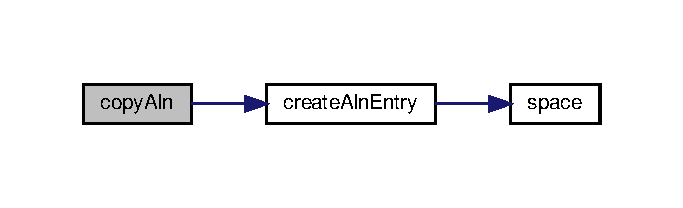
\includegraphics[width=328pt]{misc_8h_a0da1742a6a7f546827bee85fbdf53592_cgraph}
\end{center}
\end{figure}
\mbox{\Hypertarget{misc_8h_a540d653adf9134e345a0be15556bef9f}\label{misc_8h_a540d653adf9134e345a0be15556bef9f}} 
\index{misc.\+h@{misc.\+h}!copy\+Sk@{copy\+Sk}}
\index{copy\+Sk@{copy\+Sk}!misc.\+h@{misc.\+h}}
\subsubsection{\texorpdfstring{copy\+Sk()}{copySk()}}
{\footnotesize\ttfamily void copy\+Sk (\begin{DoxyParamCaption}\item[{float $\ast$$\ast$$\ast$$\ast$}]{from,  }\item[{float $\ast$$\ast$$\ast$$\ast$}]{to,  }\item[{int}]{N,  }\item[{int}]{L }\end{DoxyParamCaption})}

\mbox{\Hypertarget{misc_8h_a6017c986a43a1bba1569a8efb1b3aedb}\label{misc_8h_a6017c986a43a1bba1569a8efb1b3aedb}} 
\index{misc.\+h@{misc.\+h}!extend\+Region@{extend\+Region}}
\index{extend\+Region@{extend\+Region}!misc.\+h@{misc.\+h}}
\subsubsection{\texorpdfstring{extend\+Region()}{extendRegion()}}
{\footnotesize\ttfamily int extend\+Region (\begin{DoxyParamCaption}\item[{\hyperlink{getopt_8c_a2c212835823e3c54a8ab6d95c652660e}{const} struct \hyperlink{structaln}{aln} $\ast$}]{alignment\mbox{[}$\,$\mbox{]},  }\item[{int}]{pos,  }\item[{int}]{direction }\end{DoxyParamCaption})}

Here is the call graph for this function\+:
\nopagebreak
\begin{figure}[H]
\begin{center}
\leavevmode
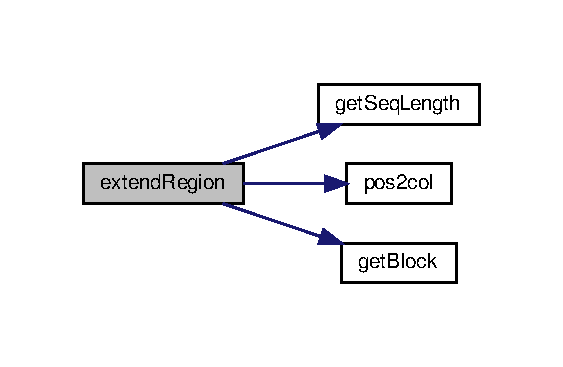
\includegraphics[width=270pt]{misc_8h_a6017c986a43a1bba1569a8efb1b3aedb_cgraph}
\end{center}
\end{figure}
\mbox{\Hypertarget{misc_8h_a71b140f8ccd1190776a6cc04f42f7b0d}\label{misc_8h_a71b140f8ccd1190776a6cc04f42f7b0d}} 
\index{misc.\+h@{misc.\+h}!free\+Results@{free\+Results}}
\index{free\+Results@{free\+Results}!misc.\+h@{misc.\+h}}
\subsubsection{\texorpdfstring{free\+Results()}{freeResults()}}
{\footnotesize\ttfamily void free\+Results (\begin{DoxyParamCaption}\item[{\hyperlink{score_8h_a5b7f5df9506ff8c871dc49e4bf9f22af}{segment\+Stats}}]{results\mbox{[}$\,$\mbox{]} }\end{DoxyParamCaption})}

\mbox{\Hypertarget{misc_8h_af625860d4b3644771a9b58a316518d00}\label{misc_8h_af625860d4b3644771a9b58a316518d00}} 
\index{misc.\+h@{misc.\+h}!gaussian@{gaussian}}
\index{gaussian@{gaussian}!misc.\+h@{misc.\+h}}
\subsubsection{\texorpdfstring{gaussian()}{gaussian()}}
{\footnotesize\ttfamily float gaussian (\begin{DoxyParamCaption}\item[{\hyperlink{getopt_8c_a2c212835823e3c54a8ab6d95c652660e}{const} float}]{sigma }\end{DoxyParamCaption})}

\mbox{\Hypertarget{misc_8h_a9fe543fe19ab3ff4ae9def519e1f0ac1}\label{misc_8h_a9fe543fe19ab3ff4ae9def519e1f0ac1}} 
\index{misc.\+h@{misc.\+h}!get\+Block@{get\+Block}}
\index{get\+Block@{get\+Block}!misc.\+h@{misc.\+h}}
\subsubsection{\texorpdfstring{get\+Block()}{getBlock()}}
{\footnotesize\ttfamily void get\+Block (\begin{DoxyParamCaption}\item[{int}]{i,  }\item[{\hyperlink{getopt_8c_a2c212835823e3c54a8ab6d95c652660e}{const} char $\ast$}]{seq\+\_\+0,  }\item[{\hyperlink{getopt_8c_a2c212835823e3c54a8ab6d95c652660e}{const} char $\ast$}]{seq\+\_\+k,  }\item[{\hyperlink{getopt_8c_a2c212835823e3c54a8ab6d95c652660e}{const} int $\ast$}]{map\+\_\+0,  }\item[{\hyperlink{getopt_8c_a2c212835823e3c54a8ab6d95c652660e}{const} int $\ast$}]{map\+\_\+k,  }\item[{char $\ast$}]{block\+\_\+0,  }\item[{char $\ast$}]{block\+\_\+k,  }\item[{int $\ast$}]{z }\end{DoxyParamCaption})}

\mbox{\Hypertarget{misc_8h_a935b3901ff2b656c44257b4606ceab6c}\label{misc_8h_a935b3901ff2b656c44257b4606ceab6c}} 
\index{misc.\+h@{misc.\+h}!get\+Seq\+Length@{get\+Seq\+Length}}
\index{get\+Seq\+Length@{get\+Seq\+Length}!misc.\+h@{misc.\+h}}
\subsubsection{\texorpdfstring{get\+Seq\+Length()}{getSeqLength()}}
{\footnotesize\ttfamily int get\+Seq\+Length (\begin{DoxyParamCaption}\item[{char $\ast$}]{seq }\end{DoxyParamCaption})}

\mbox{\Hypertarget{misc_8h_a62dbd6f5f78b8829c91c5e373b897f67}\label{misc_8h_a62dbd6f5f78b8829c91c5e373b897f67}} 
\index{misc.\+h@{misc.\+h}!h\+Dist@{h\+Dist}}
\index{h\+Dist@{h\+Dist}!misc.\+h@{misc.\+h}}
\subsubsection{\texorpdfstring{h\+Dist()}{hDist()}}
{\footnotesize\ttfamily int h\+Dist (\begin{DoxyParamCaption}\item[{int}]{a1,  }\item[{int}]{a2,  }\item[{int}]{a3,  }\item[{int}]{b1,  }\item[{int}]{b2,  }\item[{int}]{b3 }\end{DoxyParamCaption})}

\mbox{\Hypertarget{misc_8h_af49091737065e3ea21101edf17533dcf}\label{misc_8h_af49091737065e3ea21101edf17533dcf}} 
\index{misc.\+h@{misc.\+h}!pos2col@{pos2col}}
\index{pos2col@{pos2col}!misc.\+h@{misc.\+h}}
\subsubsection{\texorpdfstring{pos2col()}{pos2col()}}
{\footnotesize\ttfamily int pos2col (\begin{DoxyParamCaption}\item[{\hyperlink{getopt_8c_a2c212835823e3c54a8ab6d95c652660e}{const} char $\ast$}]{seq,  }\item[{int}]{pos }\end{DoxyParamCaption})}

\mbox{\Hypertarget{misc_8h_a622e2235405d5fce48465d284271642c}\label{misc_8h_a622e2235405d5fce48465d284271642c}} 
\index{misc.\+h@{misc.\+h}!print\+Aln\+Clustal@{print\+Aln\+Clustal}}
\index{print\+Aln\+Clustal@{print\+Aln\+Clustal}!misc.\+h@{misc.\+h}}
\subsubsection{\texorpdfstring{print\+Aln\+Clustal()}{printAlnClustal()}}
{\footnotesize\ttfamily void print\+Aln\+Clustal (\begin{DoxyParamCaption}\item[{F\+I\+LE $\ast$}]{out,  }\item[{\hyperlink{getopt_8c_a2c212835823e3c54a8ab6d95c652660e}{const} struct \hyperlink{structaln}{aln} $\ast$}]{AS\mbox{[}$\,$\mbox{]} }\end{DoxyParamCaption})}

\mbox{\Hypertarget{misc_8h_a92f776363f89ffb2864dc72fa7c8471f}\label{misc_8h_a92f776363f89ffb2864dc72fa7c8471f}} 
\index{misc.\+h@{misc.\+h}!print\+Results@{print\+Results}}
\index{print\+Results@{print\+Results}!misc.\+h@{misc.\+h}}
\subsubsection{\texorpdfstring{print\+Results()}{printResults()}}
{\footnotesize\ttfamily void print\+Results (\begin{DoxyParamCaption}\item[{F\+I\+LE $\ast$}]{outfile,  }\item[{int}]{output\+Format,  }\item[{\hyperlink{getopt_8c_a2c212835823e3c54a8ab6d95c652660e}{const} struct \hyperlink{structaln}{aln} $\ast$}]{AS\mbox{[}$\,$\mbox{]},  }\item[{\hyperlink{score_8h_a5b7f5df9506ff8c871dc49e4bf9f22af}{segment\+Stats}}]{results\mbox{[}$\,$\mbox{]} }\end{DoxyParamCaption})}

Here is the call graph for this function\+:
\nopagebreak
\begin{figure}[H]
\begin{center}
\leavevmode
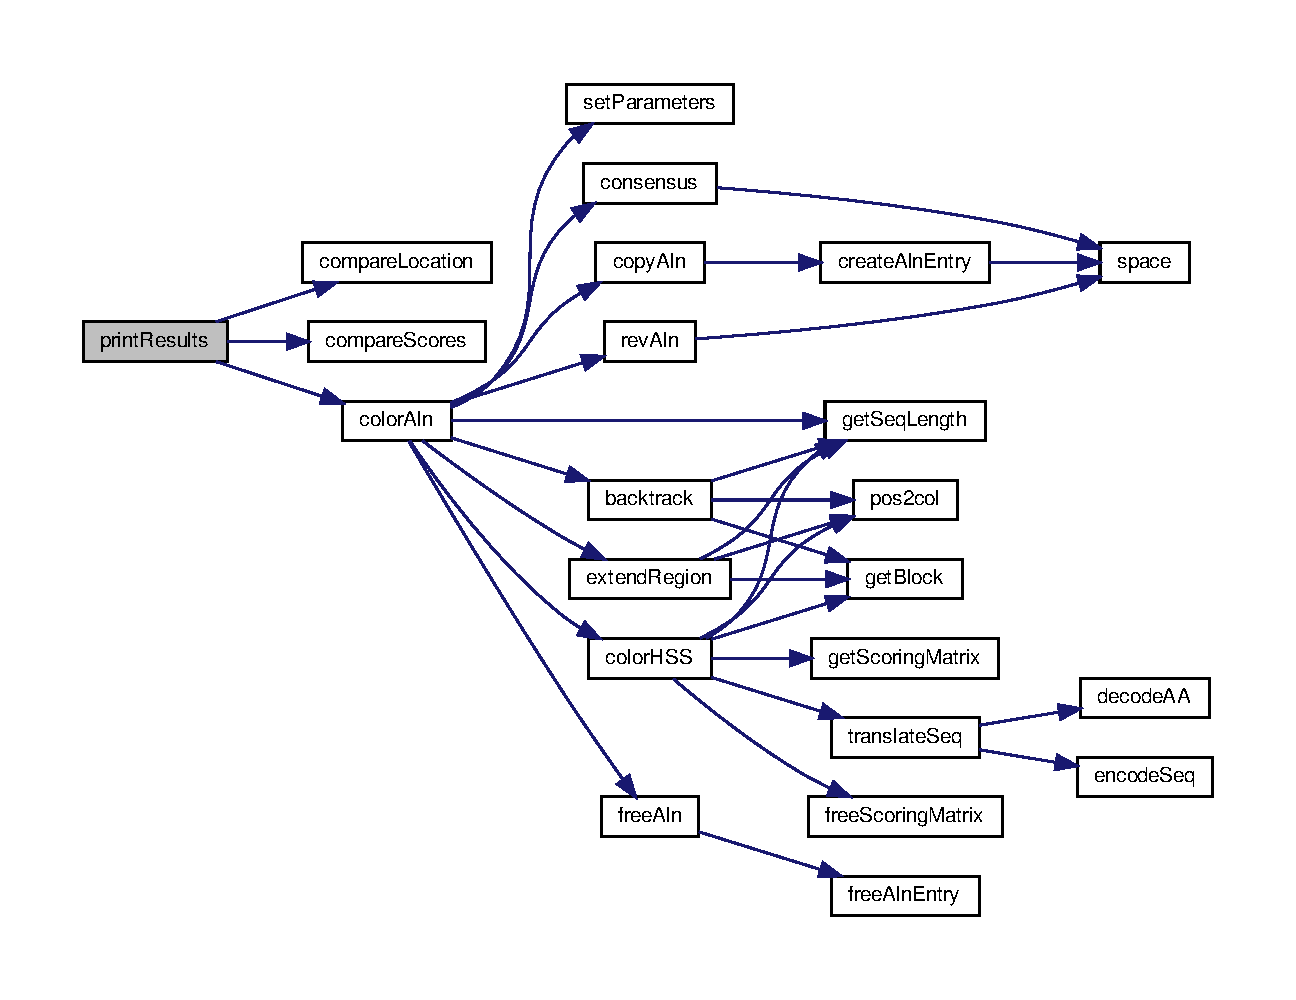
\includegraphics[width=350pt]{misc_8h_a92f776363f89ffb2864dc72fa7c8471f_cgraph}
\end{center}
\end{figure}
\mbox{\Hypertarget{misc_8h_a8eed68ed1197df02c8b9a49264efc717}\label{misc_8h_a8eed68ed1197df02c8b9a49264efc717}} 
\index{misc.\+h@{misc.\+h}!reintroduce\+Gaps@{reintroduce\+Gaps}}
\index{reintroduce\+Gaps@{reintroduce\+Gaps}!misc.\+h@{misc.\+h}}
\subsubsection{\texorpdfstring{reintroduce\+Gaps()}{reintroduceGaps()}}
{\footnotesize\ttfamily void reintroduce\+Gaps (\begin{DoxyParamCaption}\item[{\hyperlink{getopt_8c_a2c212835823e3c54a8ab6d95c652660e}{const} struct \hyperlink{structaln}{aln} $\ast$}]{orig\+Aln\mbox{[}$\,$\mbox{]},  }\item[{struct \hyperlink{structaln}{aln} $\ast$}]{sampled\+Aln\mbox{[}$\,$\mbox{]} }\end{DoxyParamCaption})}

\mbox{\Hypertarget{misc_8h_a5753372a1a3c3974fc6be9a6030a67bf}\label{misc_8h_a5753372a1a3c3974fc6be9a6030a67bf}} 
\index{misc.\+h@{misc.\+h}!sort\+Aln@{sort\+Aln}}
\index{sort\+Aln@{sort\+Aln}!misc.\+h@{misc.\+h}}
\subsubsection{\texorpdfstring{sort\+Aln()}{sortAln()}}
{\footnotesize\ttfamily void sort\+Aln (\begin{DoxyParamCaption}\item[{\hyperlink{getopt_8c_a2c212835823e3c54a8ab6d95c652660e}{const} struct \hyperlink{structaln}{aln} $\ast$}]{orig\+Aln\mbox{[}$\,$\mbox{]},  }\item[{struct \hyperlink{structaln}{aln} $\ast$}]{sampled\+Aln\mbox{[}$\,$\mbox{]} }\end{DoxyParamCaption})}

\mbox{\Hypertarget{misc_8h_ac9b591bdb26f6a8b8ee56aee3e809c65}\label{misc_8h_ac9b591bdb26f6a8b8ee56aee3e809c65}} 
\index{misc.\+h@{misc.\+h}!stddev@{stddev}}
\index{stddev@{stddev}!misc.\+h@{misc.\+h}}
\subsubsection{\texorpdfstring{stddev()}{stddev()}}
{\footnotesize\ttfamily float stddev (\begin{DoxyParamCaption}\item[{float $\ast$}]{data,  }\item[{int}]{N }\end{DoxyParamCaption})}


\hypertarget{postscript_8c}{}\section{postscript.\+c File Reference}
\label{postscript_8c}\index{postscript.\+c@{postscript.\+c}}
{\ttfamily \#include $<$string.\+h$>$}\newline
{\ttfamily \#include $<$stdio.\+h$>$}\newline
{\ttfamily \#include $<$stdlib.\+h$>$}\newline
{\ttfamily \#include $<$math.\+h$>$}\newline
{\ttfamily \#include \char`\"{}score.\+h\char`\"{}}\newline
{\ttfamily \#include \char`\"{}code.\+h\char`\"{}}\newline
{\ttfamily \#include \char`\"{}misc.\+h\char`\"{}}\newline
{\ttfamily \#include \char`\"{}postscript.\+h\char`\"{}}\newline
Include dependency graph for postscript.\+c\+:
\nopagebreak
\begin{figure}[H]
\begin{center}
\leavevmode
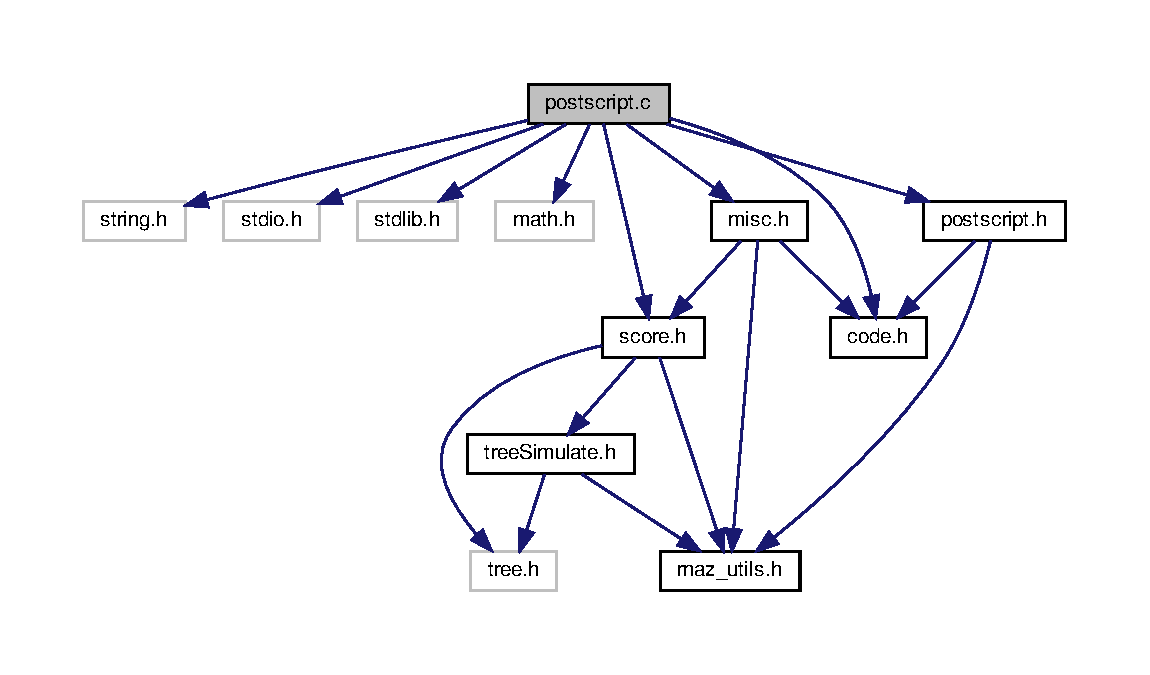
\includegraphics[width=350pt]{postscript_8c__incl}
\end{center}
\end{figure}
\subsection*{Functions}
\begin{DoxyCompactItemize}
\item 
void \hyperlink{postscript_8c_a1d6c94586a33965dd4277c7fe62de430}{set\+Parameters} ()
\item 
int \hyperlink{postscript_8c_ac7d6bf70e040d36788b6eacace4cb312}{color\+Aln} (\hyperlink{getopt_8c_a2c212835823e3c54a8ab6d95c652660e}{const} char $\ast$filename, \hyperlink{getopt_8c_a2c212835823e3c54a8ab6d95c652660e}{const} struct \hyperlink{structaln}{aln} $\ast$alignment\mbox{[}$\,$\mbox{]}, \hyperlink{score_8h_a5b7f5df9506ff8c871dc49e4bf9f22af}{segment\+Stats} region)
\item 
void \hyperlink{postscript_8c_a88d8c5c3031b8ee553b4bfc437e4b73e}{color\+H\+SS} (\hyperlink{getopt_8c_a2c212835823e3c54a8ab6d95c652660e}{const} char $\ast$filename, \hyperlink{getopt_8c_a2c212835823e3c54a8ab6d95c652660e}{const} struct \hyperlink{structaln}{aln} $\ast$alignment\mbox{[}$\,$\mbox{]}, \hyperlink{score_8h_a0751e1c4932f95e3e60c73409408a97f}{backtrack\+Data} $\ast$bt, \hyperlink{getopt_8c_a2c212835823e3c54a8ab6d95c652660e}{const} char $\ast$label, int b, int i)
\end{DoxyCompactItemize}
\subsection*{Variables}
\begin{DoxyCompactItemize}
\item 
float \hyperlink{postscript_8c_a05a25f17ddf6ed395c481d783d1af2b4}{font\+Width}
\item 
float \hyperlink{postscript_8c_a8fc5219f9ead102b3596111331374b2f}{font\+Height}
\item 
float \hyperlink{postscript_8c_a97b51530ccb867cc13f911e57be3a559}{image\+Height}
\item 
float \hyperlink{postscript_8c_a056677386b85246c5b6f9de91327868c}{image\+Width}
\item 
float \hyperlink{postscript_8c_a7e166443fa8165daca1829477a3678c1}{tmp\+Columns}
\item 
int \hyperlink{postscript_8c_a9f59b34b1f25fe00023291b678246bcc}{length}
\item 
int \hyperlink{postscript_8c_a04c4ce9dea57def69ca277c748f1ec4a}{max\+Name}
\item 
int \hyperlink{postscript_8c_af4b91d5ea883f66de1f385aee64a0d5f}{max\+Num}
\item 
int \hyperlink{postscript_8c_aee13643f97e046b7492876910b23b59d}{curr\+Pos}
\item 
int \hyperlink{postscript_8c_acb1a982424fe4ce17865ade904f6afbb}{column\+Width}
\item 
float \hyperlink{postscript_8c_a47c6c3302e0a9d686ba540869d4f3688}{line\+Step}
\item 
float \hyperlink{postscript_8c_a2d6e8a7836bfad8586715c3bb775cbb4}{block\+Step}
\item 
float \hyperlink{postscript_8c_a6290c97dafee311a97e747d02251da9d}{cons\+Step}
\item 
float \hyperlink{postscript_8c_a0fa03894e3a7c9aa3690c217af65c7c3}{ss\+Step}
\item 
float \hyperlink{postscript_8c_adbb97a02a7e2f5bc69940fc230062839}{ruler\+Step}
\item 
float \hyperlink{postscript_8c_a7b9ed0953c4c3a72b4763f3913467d83}{name\+Step}
\item 
float \hyperlink{postscript_8c_ab2e008e977e58c17747a69818f653584}{number\+Step}
\item 
float \hyperlink{postscript_8c_a0c4c0a1f79429ea034c156318b576175}{max\+Cons\+Bar}
\item 
float \hyperlink{postscript_8c_aa3dfc2d68f6a44a7941b7e6f2940ecac}{startY}
\item 
float \hyperlink{postscript_8c_ab9e364a4cf29b5aad82e7ec316ac09e9}{namesX}
\item 
float \hyperlink{postscript_8c_a69294d581be62ee920a2ef6622500cbd}{seqsX}
\item 
float \hyperlink{postscript_8c_a6cd3947c7e694dc9a6516a4efce1c73d}{currY}
\item 
F\+I\+LE $\ast$ \hyperlink{postscript_8c_ae581849c67336453bd5b81e6518019a9}{outfile}
\item 
float $\ast$$\ast$$\ast$$\ast$ \hyperlink{postscript_8c_a189ec0118947b93b0df1359ab643d3ce}{Sk\+\_\+native}
\item 
float $\ast$$\ast$$\ast$$\ast$ \hyperlink{postscript_8c_a720f3e09e87f08ee95fd84af1c9c575e}{Sk\+\_\+native\+\_\+rev}
\end{DoxyCompactItemize}


\subsection{Function Documentation}
\mbox{\Hypertarget{postscript_8c_ac7d6bf70e040d36788b6eacace4cb312}\label{postscript_8c_ac7d6bf70e040d36788b6eacace4cb312}} 
\index{postscript.\+c@{postscript.\+c}!color\+Aln@{color\+Aln}}
\index{color\+Aln@{color\+Aln}!postscript.\+c@{postscript.\+c}}
\subsubsection{\texorpdfstring{color\+Aln()}{colorAln()}}
{\footnotesize\ttfamily int color\+Aln (\begin{DoxyParamCaption}\item[{\hyperlink{getopt_8c_a2c212835823e3c54a8ab6d95c652660e}{const} char $\ast$}]{filename,  }\item[{\hyperlink{getopt_8c_a2c212835823e3c54a8ab6d95c652660e}{const} struct \hyperlink{structaln}{aln} $\ast$}]{alignment\mbox{[}$\,$\mbox{]},  }\item[{\hyperlink{score_8h_a5b7f5df9506ff8c871dc49e4bf9f22af}{segment\+Stats}}]{region }\end{DoxyParamCaption})}

Here is the call graph for this function\+:
\nopagebreak
\begin{figure}[H]
\begin{center}
\leavevmode
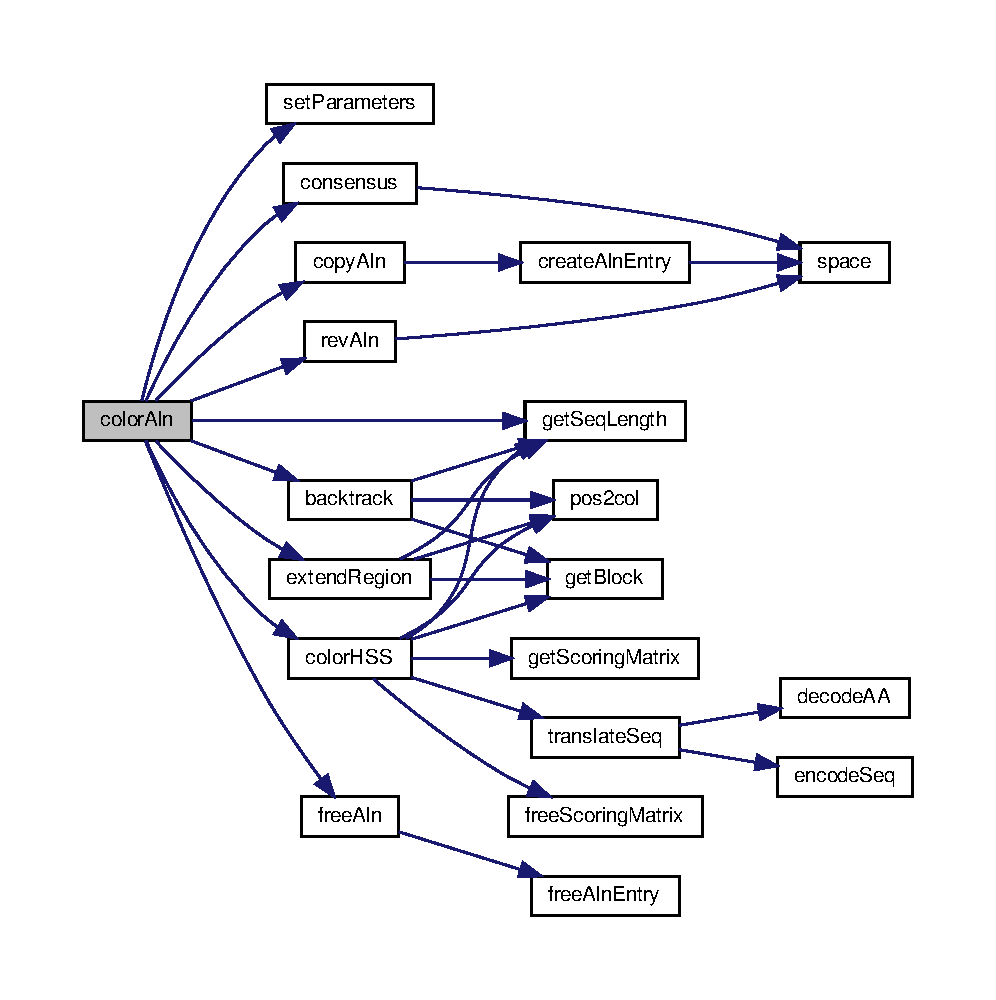
\includegraphics[width=350pt]{postscript_8c_ac7d6bf70e040d36788b6eacace4cb312_cgraph}
\end{center}
\end{figure}
\mbox{\Hypertarget{postscript_8c_a88d8c5c3031b8ee553b4bfc437e4b73e}\label{postscript_8c_a88d8c5c3031b8ee553b4bfc437e4b73e}} 
\index{postscript.\+c@{postscript.\+c}!color\+H\+SS@{color\+H\+SS}}
\index{color\+H\+SS@{color\+H\+SS}!postscript.\+c@{postscript.\+c}}
\subsubsection{\texorpdfstring{color\+H\+S\+S()}{colorHSS()}}
{\footnotesize\ttfamily void color\+H\+SS (\begin{DoxyParamCaption}\item[{\hyperlink{getopt_8c_a2c212835823e3c54a8ab6d95c652660e}{const} char $\ast$}]{filename,  }\item[{\hyperlink{getopt_8c_a2c212835823e3c54a8ab6d95c652660e}{const} struct \hyperlink{structaln}{aln} $\ast$}]{alignment\mbox{[}$\,$\mbox{]},  }\item[{\hyperlink{score_8h_a0751e1c4932f95e3e60c73409408a97f}{backtrack\+Data} $\ast$}]{bt,  }\item[{\hyperlink{getopt_8c_a2c212835823e3c54a8ab6d95c652660e}{const} char $\ast$}]{label,  }\item[{int}]{b,  }\item[{int}]{i }\end{DoxyParamCaption})}

Here is the call graph for this function\+:
\nopagebreak
\begin{figure}[H]
\begin{center}
\leavevmode
\includegraphics[width=350pt]{postscript_8c_a88d8c5c3031b8ee553b4bfc437e4b73e_cgraph}
\end{center}
\end{figure}
\mbox{\Hypertarget{postscript_8c_a1d6c94586a33965dd4277c7fe62de430}\label{postscript_8c_a1d6c94586a33965dd4277c7fe62de430}} 
\index{postscript.\+c@{postscript.\+c}!set\+Parameters@{set\+Parameters}}
\index{set\+Parameters@{set\+Parameters}!postscript.\+c@{postscript.\+c}}
\subsubsection{\texorpdfstring{set\+Parameters()}{setParameters()}}
{\footnotesize\ttfamily void set\+Parameters (\begin{DoxyParamCaption}{ }\end{DoxyParamCaption})}



\subsection{Variable Documentation}
\mbox{\Hypertarget{postscript_8c_a2d6e8a7836bfad8586715c3bb775cbb4}\label{postscript_8c_a2d6e8a7836bfad8586715c3bb775cbb4}} 
\index{postscript.\+c@{postscript.\+c}!block\+Step@{block\+Step}}
\index{block\+Step@{block\+Step}!postscript.\+c@{postscript.\+c}}
\subsubsection{\texorpdfstring{block\+Step}{blockStep}}
{\footnotesize\ttfamily float block\+Step}

\mbox{\Hypertarget{postscript_8c_acb1a982424fe4ce17865ade904f6afbb}\label{postscript_8c_acb1a982424fe4ce17865ade904f6afbb}} 
\index{postscript.\+c@{postscript.\+c}!column\+Width@{column\+Width}}
\index{column\+Width@{column\+Width}!postscript.\+c@{postscript.\+c}}
\subsubsection{\texorpdfstring{column\+Width}{columnWidth}}
{\footnotesize\ttfamily int column\+Width}

\mbox{\Hypertarget{postscript_8c_a6290c97dafee311a97e747d02251da9d}\label{postscript_8c_a6290c97dafee311a97e747d02251da9d}} 
\index{postscript.\+c@{postscript.\+c}!cons\+Step@{cons\+Step}}
\index{cons\+Step@{cons\+Step}!postscript.\+c@{postscript.\+c}}
\subsubsection{\texorpdfstring{cons\+Step}{consStep}}
{\footnotesize\ttfamily float cons\+Step}

\mbox{\Hypertarget{postscript_8c_aee13643f97e046b7492876910b23b59d}\label{postscript_8c_aee13643f97e046b7492876910b23b59d}} 
\index{postscript.\+c@{postscript.\+c}!curr\+Pos@{curr\+Pos}}
\index{curr\+Pos@{curr\+Pos}!postscript.\+c@{postscript.\+c}}
\subsubsection{\texorpdfstring{curr\+Pos}{currPos}}
{\footnotesize\ttfamily int curr\+Pos}

\mbox{\Hypertarget{postscript_8c_a6cd3947c7e694dc9a6516a4efce1c73d}\label{postscript_8c_a6cd3947c7e694dc9a6516a4efce1c73d}} 
\index{postscript.\+c@{postscript.\+c}!currY@{currY}}
\index{currY@{currY}!postscript.\+c@{postscript.\+c}}
\subsubsection{\texorpdfstring{currY}{currY}}
{\footnotesize\ttfamily float currY}

\mbox{\Hypertarget{postscript_8c_a8fc5219f9ead102b3596111331374b2f}\label{postscript_8c_a8fc5219f9ead102b3596111331374b2f}} 
\index{postscript.\+c@{postscript.\+c}!font\+Height@{font\+Height}}
\index{font\+Height@{font\+Height}!postscript.\+c@{postscript.\+c}}
\subsubsection{\texorpdfstring{font\+Height}{fontHeight}}
{\footnotesize\ttfamily float font\+Height}

\mbox{\Hypertarget{postscript_8c_a05a25f17ddf6ed395c481d783d1af2b4}\label{postscript_8c_a05a25f17ddf6ed395c481d783d1af2b4}} 
\index{postscript.\+c@{postscript.\+c}!font\+Width@{font\+Width}}
\index{font\+Width@{font\+Width}!postscript.\+c@{postscript.\+c}}
\subsubsection{\texorpdfstring{font\+Width}{fontWidth}}
{\footnotesize\ttfamily float font\+Width}

\mbox{\Hypertarget{postscript_8c_a97b51530ccb867cc13f911e57be3a559}\label{postscript_8c_a97b51530ccb867cc13f911e57be3a559}} 
\index{postscript.\+c@{postscript.\+c}!image\+Height@{image\+Height}}
\index{image\+Height@{image\+Height}!postscript.\+c@{postscript.\+c}}
\subsubsection{\texorpdfstring{image\+Height}{imageHeight}}
{\footnotesize\ttfamily float image\+Height}

\mbox{\Hypertarget{postscript_8c_a056677386b85246c5b6f9de91327868c}\label{postscript_8c_a056677386b85246c5b6f9de91327868c}} 
\index{postscript.\+c@{postscript.\+c}!image\+Width@{image\+Width}}
\index{image\+Width@{image\+Width}!postscript.\+c@{postscript.\+c}}
\subsubsection{\texorpdfstring{image\+Width}{imageWidth}}
{\footnotesize\ttfamily float image\+Width}

\mbox{\Hypertarget{postscript_8c_a9f59b34b1f25fe00023291b678246bcc}\label{postscript_8c_a9f59b34b1f25fe00023291b678246bcc}} 
\index{postscript.\+c@{postscript.\+c}!length@{length}}
\index{length@{length}!postscript.\+c@{postscript.\+c}}
\subsubsection{\texorpdfstring{length}{length}}
{\footnotesize\ttfamily int length}

\mbox{\Hypertarget{postscript_8c_a47c6c3302e0a9d686ba540869d4f3688}\label{postscript_8c_a47c6c3302e0a9d686ba540869d4f3688}} 
\index{postscript.\+c@{postscript.\+c}!line\+Step@{line\+Step}}
\index{line\+Step@{line\+Step}!postscript.\+c@{postscript.\+c}}
\subsubsection{\texorpdfstring{line\+Step}{lineStep}}
{\footnotesize\ttfamily float line\+Step}

\mbox{\Hypertarget{postscript_8c_a0c4c0a1f79429ea034c156318b576175}\label{postscript_8c_a0c4c0a1f79429ea034c156318b576175}} 
\index{postscript.\+c@{postscript.\+c}!max\+Cons\+Bar@{max\+Cons\+Bar}}
\index{max\+Cons\+Bar@{max\+Cons\+Bar}!postscript.\+c@{postscript.\+c}}
\subsubsection{\texorpdfstring{max\+Cons\+Bar}{maxConsBar}}
{\footnotesize\ttfamily float max\+Cons\+Bar}

\mbox{\Hypertarget{postscript_8c_a04c4ce9dea57def69ca277c748f1ec4a}\label{postscript_8c_a04c4ce9dea57def69ca277c748f1ec4a}} 
\index{postscript.\+c@{postscript.\+c}!max\+Name@{max\+Name}}
\index{max\+Name@{max\+Name}!postscript.\+c@{postscript.\+c}}
\subsubsection{\texorpdfstring{max\+Name}{maxName}}
{\footnotesize\ttfamily int max\+Name}

\mbox{\Hypertarget{postscript_8c_af4b91d5ea883f66de1f385aee64a0d5f}\label{postscript_8c_af4b91d5ea883f66de1f385aee64a0d5f}} 
\index{postscript.\+c@{postscript.\+c}!max\+Num@{max\+Num}}
\index{max\+Num@{max\+Num}!postscript.\+c@{postscript.\+c}}
\subsubsection{\texorpdfstring{max\+Num}{maxNum}}
{\footnotesize\ttfamily int max\+Num}

\mbox{\Hypertarget{postscript_8c_a7b9ed0953c4c3a72b4763f3913467d83}\label{postscript_8c_a7b9ed0953c4c3a72b4763f3913467d83}} 
\index{postscript.\+c@{postscript.\+c}!name\+Step@{name\+Step}}
\index{name\+Step@{name\+Step}!postscript.\+c@{postscript.\+c}}
\subsubsection{\texorpdfstring{name\+Step}{nameStep}}
{\footnotesize\ttfamily float name\+Step}

\mbox{\Hypertarget{postscript_8c_ab9e364a4cf29b5aad82e7ec316ac09e9}\label{postscript_8c_ab9e364a4cf29b5aad82e7ec316ac09e9}} 
\index{postscript.\+c@{postscript.\+c}!namesX@{namesX}}
\index{namesX@{namesX}!postscript.\+c@{postscript.\+c}}
\subsubsection{\texorpdfstring{namesX}{namesX}}
{\footnotesize\ttfamily float namesX}

\mbox{\Hypertarget{postscript_8c_ab2e008e977e58c17747a69818f653584}\label{postscript_8c_ab2e008e977e58c17747a69818f653584}} 
\index{postscript.\+c@{postscript.\+c}!number\+Step@{number\+Step}}
\index{number\+Step@{number\+Step}!postscript.\+c@{postscript.\+c}}
\subsubsection{\texorpdfstring{number\+Step}{numberStep}}
{\footnotesize\ttfamily float number\+Step}

\mbox{\Hypertarget{postscript_8c_ae581849c67336453bd5b81e6518019a9}\label{postscript_8c_ae581849c67336453bd5b81e6518019a9}} 
\index{postscript.\+c@{postscript.\+c}!outfile@{outfile}}
\index{outfile@{outfile}!postscript.\+c@{postscript.\+c}}
\subsubsection{\texorpdfstring{outfile}{outfile}}
{\footnotesize\ttfamily F\+I\+LE$\ast$ outfile}

\mbox{\Hypertarget{postscript_8c_adbb97a02a7e2f5bc69940fc230062839}\label{postscript_8c_adbb97a02a7e2f5bc69940fc230062839}} 
\index{postscript.\+c@{postscript.\+c}!ruler\+Step@{ruler\+Step}}
\index{ruler\+Step@{ruler\+Step}!postscript.\+c@{postscript.\+c}}
\subsubsection{\texorpdfstring{ruler\+Step}{rulerStep}}
{\footnotesize\ttfamily float ruler\+Step}

\mbox{\Hypertarget{postscript_8c_a69294d581be62ee920a2ef6622500cbd}\label{postscript_8c_a69294d581be62ee920a2ef6622500cbd}} 
\index{postscript.\+c@{postscript.\+c}!seqsX@{seqsX}}
\index{seqsX@{seqsX}!postscript.\+c@{postscript.\+c}}
\subsubsection{\texorpdfstring{seqsX}{seqsX}}
{\footnotesize\ttfamily float seqsX}

\mbox{\Hypertarget{postscript_8c_a189ec0118947b93b0df1359ab643d3ce}\label{postscript_8c_a189ec0118947b93b0df1359ab643d3ce}} 
\index{postscript.\+c@{postscript.\+c}!Sk\+\_\+native@{Sk\+\_\+native}}
\index{Sk\+\_\+native@{Sk\+\_\+native}!postscript.\+c@{postscript.\+c}}
\subsubsection{\texorpdfstring{Sk\+\_\+native}{Sk\_native}}
{\footnotesize\ttfamily float$\ast$$\ast$$\ast$$\ast$ Sk\+\_\+native}

\mbox{\Hypertarget{postscript_8c_a720f3e09e87f08ee95fd84af1c9c575e}\label{postscript_8c_a720f3e09e87f08ee95fd84af1c9c575e}} 
\index{postscript.\+c@{postscript.\+c}!Sk\+\_\+native\+\_\+rev@{Sk\+\_\+native\+\_\+rev}}
\index{Sk\+\_\+native\+\_\+rev@{Sk\+\_\+native\+\_\+rev}!postscript.\+c@{postscript.\+c}}
\subsubsection{\texorpdfstring{Sk\+\_\+native\+\_\+rev}{Sk\_native\_rev}}
{\footnotesize\ttfamily float$\ast$$\ast$$\ast$$\ast$ Sk\+\_\+native\+\_\+rev}

\mbox{\Hypertarget{postscript_8c_a0fa03894e3a7c9aa3690c217af65c7c3}\label{postscript_8c_a0fa03894e3a7c9aa3690c217af65c7c3}} 
\index{postscript.\+c@{postscript.\+c}!ss\+Step@{ss\+Step}}
\index{ss\+Step@{ss\+Step}!postscript.\+c@{postscript.\+c}}
\subsubsection{\texorpdfstring{ss\+Step}{ssStep}}
{\footnotesize\ttfamily float ss\+Step}

\mbox{\Hypertarget{postscript_8c_aa3dfc2d68f6a44a7941b7e6f2940ecac}\label{postscript_8c_aa3dfc2d68f6a44a7941b7e6f2940ecac}} 
\index{postscript.\+c@{postscript.\+c}!startY@{startY}}
\index{startY@{startY}!postscript.\+c@{postscript.\+c}}
\subsubsection{\texorpdfstring{startY}{startY}}
{\footnotesize\ttfamily float startY}

\mbox{\Hypertarget{postscript_8c_a7e166443fa8165daca1829477a3678c1}\label{postscript_8c_a7e166443fa8165daca1829477a3678c1}} 
\index{postscript.\+c@{postscript.\+c}!tmp\+Columns@{tmp\+Columns}}
\index{tmp\+Columns@{tmp\+Columns}!postscript.\+c@{postscript.\+c}}
\subsubsection{\texorpdfstring{tmp\+Columns}{tmpColumns}}
{\footnotesize\ttfamily float tmp\+Columns}


\hypertarget{postscript_8h}{}\section{postscript.\+h File Reference}
\label{postscript_8h}\index{postscript.\+h@{postscript.\+h}}
{\ttfamily \#include \char`\"{}rnaz\+\_\+utils.\+h\char`\"{}}\newline
{\ttfamily \#include \char`\"{}code.\+h\char`\"{}}\newline
Include dependency graph for postscript.\+h\+:
\nopagebreak
\begin{figure}[H]
\begin{center}
\leavevmode
\includegraphics[width=212pt]{postscript_8h__incl}
\end{center}
\end{figure}
This graph shows which files directly or indirectly include this file\+:
\nopagebreak
\begin{figure}[H]
\begin{center}
\leavevmode
\includegraphics[width=298pt]{postscript_8h__dep__incl}
\end{center}
\end{figure}
\subsection*{Functions}
\begin{DoxyCompactItemize}
\item 
int \hyperlink{postscript_8h_ac7d6bf70e040d36788b6eacace4cb312}{color\+Aln} (\hyperlink{getopt_8c_a2c212835823e3c54a8ab6d95c652660e}{const} char $\ast$filename, \hyperlink{getopt_8c_a2c212835823e3c54a8ab6d95c652660e}{const} struct \hyperlink{structaln}{aln} $\ast$alignment\mbox{[}$\,$\mbox{]}, \hyperlink{score_8h_a5b7f5df9506ff8c871dc49e4bf9f22af}{segment\+Stats} region)
\item 
void \hyperlink{postscript_8h_a88d8c5c3031b8ee553b4bfc437e4b73e}{color\+H\+SS} (\hyperlink{getopt_8c_a2c212835823e3c54a8ab6d95c652660e}{const} char $\ast$filename, \hyperlink{getopt_8c_a2c212835823e3c54a8ab6d95c652660e}{const} struct \hyperlink{structaln}{aln} $\ast$alignment\mbox{[}$\,$\mbox{]}, \hyperlink{score_8h_a0751e1c4932f95e3e60c73409408a97f}{backtrack\+Data} $\ast$bt, \hyperlink{getopt_8c_a2c212835823e3c54a8ab6d95c652660e}{const} char $\ast$label, int b, int i)
\item 
void \hyperlink{postscript_8h_a1d6c94586a33965dd4277c7fe62de430}{set\+Parameters} ()
\end{DoxyCompactItemize}


\subsection{Function Documentation}
\mbox{\Hypertarget{postscript_8h_ac7d6bf70e040d36788b6eacace4cb312}\label{postscript_8h_ac7d6bf70e040d36788b6eacace4cb312}} 
\index{postscript.\+h@{postscript.\+h}!color\+Aln@{color\+Aln}}
\index{color\+Aln@{color\+Aln}!postscript.\+h@{postscript.\+h}}
\subsubsection{\texorpdfstring{color\+Aln()}{colorAln()}}
{\footnotesize\ttfamily int color\+Aln (\begin{DoxyParamCaption}\item[{\hyperlink{getopt_8c_a2c212835823e3c54a8ab6d95c652660e}{const} char $\ast$}]{filename,  }\item[{\hyperlink{getopt_8c_a2c212835823e3c54a8ab6d95c652660e}{const} struct \hyperlink{structaln}{aln} $\ast$}]{alignment\mbox{[}$\,$\mbox{]},  }\item[{\hyperlink{score_8h_a5b7f5df9506ff8c871dc49e4bf9f22af}{segment\+Stats}}]{region }\end{DoxyParamCaption})}

Here is the call graph for this function\+:
\nopagebreak
\begin{figure}[H]
\begin{center}
\leavevmode
\includegraphics[width=350pt]{postscript_8h_ac7d6bf70e040d36788b6eacace4cb312_cgraph}
\end{center}
\end{figure}
\mbox{\Hypertarget{postscript_8h_a88d8c5c3031b8ee553b4bfc437e4b73e}\label{postscript_8h_a88d8c5c3031b8ee553b4bfc437e4b73e}} 
\index{postscript.\+h@{postscript.\+h}!color\+H\+SS@{color\+H\+SS}}
\index{color\+H\+SS@{color\+H\+SS}!postscript.\+h@{postscript.\+h}}
\subsubsection{\texorpdfstring{color\+H\+S\+S()}{colorHSS()}}
{\footnotesize\ttfamily void color\+H\+SS (\begin{DoxyParamCaption}\item[{\hyperlink{getopt_8c_a2c212835823e3c54a8ab6d95c652660e}{const} char $\ast$}]{filename,  }\item[{\hyperlink{getopt_8c_a2c212835823e3c54a8ab6d95c652660e}{const} struct \hyperlink{structaln}{aln} $\ast$}]{alignment\mbox{[}$\,$\mbox{]},  }\item[{\hyperlink{score_8h_a0751e1c4932f95e3e60c73409408a97f}{backtrack\+Data} $\ast$}]{bt,  }\item[{\hyperlink{getopt_8c_a2c212835823e3c54a8ab6d95c652660e}{const} char $\ast$}]{label,  }\item[{int}]{b,  }\item[{int}]{i }\end{DoxyParamCaption})}

Here is the call graph for this function\+:
\nopagebreak
\begin{figure}[H]
\begin{center}
\leavevmode
\includegraphics[width=350pt]{postscript_8h_a88d8c5c3031b8ee553b4bfc437e4b73e_cgraph}
\end{center}
\end{figure}
\mbox{\Hypertarget{postscript_8h_a1d6c94586a33965dd4277c7fe62de430}\label{postscript_8h_a1d6c94586a33965dd4277c7fe62de430}} 
\index{postscript.\+h@{postscript.\+h}!set\+Parameters@{set\+Parameters}}
\index{set\+Parameters@{set\+Parameters}!postscript.\+h@{postscript.\+h}}
\subsubsection{\texorpdfstring{set\+Parameters()}{setParameters()}}
{\footnotesize\ttfamily void set\+Parameters (\begin{DoxyParamCaption}{ }\end{DoxyParamCaption})}


\hypertarget{RNAcode_8c}{}\section{R\+N\+Acode.\+c File Reference}
\label{RNAcode_8c}\index{R\+N\+Acode.\+c@{R\+N\+Acode.\+c}}
{\ttfamily \#include $<$time.\+h$>$}\newline
{\ttfamily \#include $<$stdio.\+h$>$}\newline
{\ttfamily \#include $<$stdlib.\+h$>$}\newline
{\ttfamily \#include $<$string.\+h$>$}\newline
{\ttfamily \#include $<$ctype.\+h$>$}\newline
{\ttfamily \#include $<$math.\+h$>$}\newline
{\ttfamily \#include \char`\"{}R\+N\+Acode.\+h\char`\"{}}\newline
{\ttfamily \#include \char`\"{}rnaz\+\_\+utils.\+h\char`\"{}}\newline
{\ttfamily \#include \char`\"{}tree\+M\+L.\+h\char`\"{}}\newline
{\ttfamily \#include \char`\"{}cmdline.\+h\char`\"{}}\newline
{\ttfamily \#include \char`\"{}code.\+h\char`\"{}}\newline
{\ttfamily \#include \char`\"{}score.\+h\char`\"{}}\newline
{\ttfamily \#include \char`\"{}tree.\+h\char`\"{}}\newline
{\ttfamily \#include \char`\"{}tree\+Simulate.\+h\char`\"{}}\newline
{\ttfamily \#include \char`\"{}extreme\+\_\+fit.\+h\char`\"{}}\newline
{\ttfamily \#include \char`\"{}postscript.\+h\char`\"{}}\newline
{\ttfamily \#include \char`\"{}misc.\+h\char`\"{}}\newline
{\ttfamily \#include \char`\"{}utils.\+h\char`\"{}}\newline
Include dependency graph for R\+N\+Acode.\+c\+:
\nopagebreak
\begin{figure}[H]
\begin{center}
\leavevmode
\includegraphics[width=350pt]{RNAcode_8c__incl}
\end{center}
\end{figure}
\subsection*{Functions}
\begin{DoxyCompactItemize}
\item 
void \hyperlink{RNAcode_8c_a303c139a77497eb1282c6d2a4d415c1c}{free\+Models} (\hyperlink{score_8h_aec88546fa977a827f3312b2c12738421}{bg\+Model} $\ast$\hyperlink{score_8c_a2351b02aa48f9f78d350b4b19408d38f}{models}, int N)
\item 
int \hyperlink{RNAcode_8c_a0ddf1224851353fc92bfbff6f499fa97}{main} (int argc, char $\ast$argv\mbox{[}$\,$\mbox{]})
\item 
void \hyperlink{RNAcode_8c_ae8605e2b78cd4a81b6c6b5c30cb7366a}{usage} (void)
\item 
void \hyperlink{RNAcode_8c_a0bed8474bd33a912769360766f6b10d4}{help} (void)
\item 
void \hyperlink{RNAcode_8c_af986bd0575ec9b913dfab4b8422509ae}{version} (void)
\item 
void \hyperlink{RNAcode_8c_ae36ab4408b3aaada4218ac5f60ea6027}{read\+\_\+commandline} (int argc, char $\ast$argv\mbox{[}$\,$\mbox{]})
\end{DoxyCompactItemize}
\subsection*{Variables}
\begin{DoxyCompactItemize}
\item 
\hyperlink{RNAcode_8h_ac21aeabbefffddb27496994611a09dcd}{parameters} \hyperlink{RNAcode_8c_a8dea3b88a171ed8de9f8f98079e7561a}{pars}
\item 
\hyperlink{score_8h_aec88546fa977a827f3312b2c12738421}{bg\+Model} $\ast$ \hyperlink{RNAcode_8c_a2351b02aa48f9f78d350b4b19408d38f}{models}
\item 
\hyperlink{score_8h_aec88546fa977a827f3312b2c12738421}{bg\+Model} $\ast$ \hyperlink{RNAcode_8c_aa758f546869f82fa894aeeab59fc8a4f}{models\+Rev}
\item 
float $\ast$$\ast$$\ast$$\ast$ \hyperlink{RNAcode_8c_a1662932a5f2814e67dfbbd95ab925073}{Sk}
\item 
float $\ast$$\ast$$\ast$$\ast$ \hyperlink{RNAcode_8c_a189ec0118947b93b0df1359ab643d3ce}{Sk\+\_\+native}
\item 
float $\ast$$\ast$$\ast$$\ast$ \hyperlink{RNAcode_8c_a720f3e09e87f08ee95fd84af1c9c575e}{Sk\+\_\+native\+\_\+rev}
\item 
long int \hyperlink{RNAcode_8c_a8c5872fcd4604b525d509ffd6afc5631}{hit\+Counter}
\end{DoxyCompactItemize}


\subsection{Function Documentation}
\mbox{\Hypertarget{RNAcode_8c_a303c139a77497eb1282c6d2a4d415c1c}\label{RNAcode_8c_a303c139a77497eb1282c6d2a4d415c1c}} 
\index{R\+N\+Acode.\+c@{R\+N\+Acode.\+c}!free\+Models@{free\+Models}}
\index{free\+Models@{free\+Models}!R\+N\+Acode.\+c@{R\+N\+Acode.\+c}}
\subsubsection{\texorpdfstring{free\+Models()}{freeModels()}}
{\footnotesize\ttfamily void free\+Models (\begin{DoxyParamCaption}\item[{\hyperlink{score_8h_aec88546fa977a827f3312b2c12738421}{bg\+Model} $\ast$}]{models,  }\item[{int}]{N }\end{DoxyParamCaption})}

Here is the call graph for this function\+:
\nopagebreak
\begin{figure}[H]
\begin{center}
\leavevmode
\includegraphics[width=274pt]{RNAcode_8c_a303c139a77497eb1282c6d2a4d415c1c_cgraph}
\end{center}
\end{figure}
\mbox{\Hypertarget{RNAcode_8c_a0bed8474bd33a912769360766f6b10d4}\label{RNAcode_8c_a0bed8474bd33a912769360766f6b10d4}} 
\index{R\+N\+Acode.\+c@{R\+N\+Acode.\+c}!help@{help}}
\index{help@{help}!R\+N\+Acode.\+c@{R\+N\+Acode.\+c}}
\subsubsection{\texorpdfstring{help()}{help()}}
{\footnotesize\ttfamily void help (\begin{DoxyParamCaption}\item[{void}]{ }\end{DoxyParamCaption})}

Here is the call graph for this function\+:
\nopagebreak
\begin{figure}[H]
\begin{center}
\leavevmode
\includegraphics[width=258pt]{RNAcode_8c_a0bed8474bd33a912769360766f6b10d4_cgraph}
\end{center}
\end{figure}
\mbox{\Hypertarget{RNAcode_8c_a0ddf1224851353fc92bfbff6f499fa97}\label{RNAcode_8c_a0ddf1224851353fc92bfbff6f499fa97}} 
\index{R\+N\+Acode.\+c@{R\+N\+Acode.\+c}!main@{main}}
\index{main@{main}!R\+N\+Acode.\+c@{R\+N\+Acode.\+c}}
\subsubsection{\texorpdfstring{main()}{main()}}
{\footnotesize\ttfamily int main (\begin{DoxyParamCaption}\item[{int}]{argc,  }\item[{char $\ast$}]{argv\mbox{[}$\,$\mbox{]} }\end{DoxyParamCaption})}

Here is the call graph for this function\+:
\nopagebreak
\begin{figure}[H]
\begin{center}
\leavevmode
\includegraphics[height=550pt]{RNAcode_8c_a0ddf1224851353fc92bfbff6f499fa97_cgraph}
\end{center}
\end{figure}
\mbox{\Hypertarget{RNAcode_8c_ae36ab4408b3aaada4218ac5f60ea6027}\label{RNAcode_8c_ae36ab4408b3aaada4218ac5f60ea6027}} 
\index{R\+N\+Acode.\+c@{R\+N\+Acode.\+c}!read\+\_\+commandline@{read\+\_\+commandline}}
\index{read\+\_\+commandline@{read\+\_\+commandline}!R\+N\+Acode.\+c@{R\+N\+Acode.\+c}}
\subsubsection{\texorpdfstring{read\+\_\+commandline()}{read\_commandline()}}
{\footnotesize\ttfamily void read\+\_\+commandline (\begin{DoxyParamCaption}\item[{int}]{argc,  }\item[{char $\ast$}]{argv\mbox{[}$\,$\mbox{]} }\end{DoxyParamCaption})}

Here is the call graph for this function\+:
\nopagebreak
\begin{figure}[H]
\begin{center}
\leavevmode
\includegraphics[width=350pt]{RNAcode_8c_ae36ab4408b3aaada4218ac5f60ea6027_cgraph}
\end{center}
\end{figure}
\mbox{\Hypertarget{RNAcode_8c_ae8605e2b78cd4a81b6c6b5c30cb7366a}\label{RNAcode_8c_ae8605e2b78cd4a81b6c6b5c30cb7366a}} 
\index{R\+N\+Acode.\+c@{R\+N\+Acode.\+c}!usage@{usage}}
\index{usage@{usage}!R\+N\+Acode.\+c@{R\+N\+Acode.\+c}}
\subsubsection{\texorpdfstring{usage()}{usage()}}
{\footnotesize\ttfamily void usage (\begin{DoxyParamCaption}\item[{void}]{ }\end{DoxyParamCaption})}

Here is the call graph for this function\+:
\nopagebreak
\begin{figure}[H]
\begin{center}
\leavevmode
\includegraphics[width=337pt]{RNAcode_8c_ae8605e2b78cd4a81b6c6b5c30cb7366a_cgraph}
\end{center}
\end{figure}
\mbox{\Hypertarget{RNAcode_8c_af986bd0575ec9b913dfab4b8422509ae}\label{RNAcode_8c_af986bd0575ec9b913dfab4b8422509ae}} 
\index{R\+N\+Acode.\+c@{R\+N\+Acode.\+c}!version@{version}}
\index{version@{version}!R\+N\+Acode.\+c@{R\+N\+Acode.\+c}}
\subsubsection{\texorpdfstring{version()}{version()}}
{\footnotesize\ttfamily void version (\begin{DoxyParamCaption}\item[{void}]{ }\end{DoxyParamCaption})}



\subsection{Variable Documentation}
\mbox{\Hypertarget{RNAcode_8c_a8c5872fcd4604b525d509ffd6afc5631}\label{RNAcode_8c_a8c5872fcd4604b525d509ffd6afc5631}} 
\index{R\+N\+Acode.\+c@{R\+N\+Acode.\+c}!hit\+Counter@{hit\+Counter}}
\index{hit\+Counter@{hit\+Counter}!R\+N\+Acode.\+c@{R\+N\+Acode.\+c}}
\subsubsection{\texorpdfstring{hit\+Counter}{hitCounter}}
{\footnotesize\ttfamily long int hit\+Counter}

\mbox{\Hypertarget{RNAcode_8c_a2351b02aa48f9f78d350b4b19408d38f}\label{RNAcode_8c_a2351b02aa48f9f78d350b4b19408d38f}} 
\index{R\+N\+Acode.\+c@{R\+N\+Acode.\+c}!models@{models}}
\index{models@{models}!R\+N\+Acode.\+c@{R\+N\+Acode.\+c}}
\subsubsection{\texorpdfstring{models}{models}}
{\footnotesize\ttfamily \hyperlink{score_8h_aec88546fa977a827f3312b2c12738421}{bg\+Model}$\ast$ models}

\mbox{\Hypertarget{RNAcode_8c_aa758f546869f82fa894aeeab59fc8a4f}\label{RNAcode_8c_aa758f546869f82fa894aeeab59fc8a4f}} 
\index{R\+N\+Acode.\+c@{R\+N\+Acode.\+c}!models\+Rev@{models\+Rev}}
\index{models\+Rev@{models\+Rev}!R\+N\+Acode.\+c@{R\+N\+Acode.\+c}}
\subsubsection{\texorpdfstring{models\+Rev}{modelsRev}}
{\footnotesize\ttfamily \hyperlink{score_8h_aec88546fa977a827f3312b2c12738421}{bg\+Model} $\ast$ models\+Rev}

\mbox{\Hypertarget{RNAcode_8c_a8dea3b88a171ed8de9f8f98079e7561a}\label{RNAcode_8c_a8dea3b88a171ed8de9f8f98079e7561a}} 
\index{R\+N\+Acode.\+c@{R\+N\+Acode.\+c}!pars@{pars}}
\index{pars@{pars}!R\+N\+Acode.\+c@{R\+N\+Acode.\+c}}
\subsubsection{\texorpdfstring{pars}{pars}}
{\footnotesize\ttfamily \hyperlink{RNAcode_8h_ac21aeabbefffddb27496994611a09dcd}{parameters} pars}

\mbox{\Hypertarget{RNAcode_8c_a1662932a5f2814e67dfbbd95ab925073}\label{RNAcode_8c_a1662932a5f2814e67dfbbd95ab925073}} 
\index{R\+N\+Acode.\+c@{R\+N\+Acode.\+c}!Sk@{Sk}}
\index{Sk@{Sk}!R\+N\+Acode.\+c@{R\+N\+Acode.\+c}}
\subsubsection{\texorpdfstring{Sk}{Sk}}
{\footnotesize\ttfamily float$\ast$$\ast$$\ast$$\ast$ Sk}

\mbox{\Hypertarget{RNAcode_8c_a189ec0118947b93b0df1359ab643d3ce}\label{RNAcode_8c_a189ec0118947b93b0df1359ab643d3ce}} 
\index{R\+N\+Acode.\+c@{R\+N\+Acode.\+c}!Sk\+\_\+native@{Sk\+\_\+native}}
\index{Sk\+\_\+native@{Sk\+\_\+native}!R\+N\+Acode.\+c@{R\+N\+Acode.\+c}}
\subsubsection{\texorpdfstring{Sk\+\_\+native}{Sk\_native}}
{\footnotesize\ttfamily float$\ast$$\ast$$\ast$$\ast$ Sk\+\_\+native}

\mbox{\Hypertarget{RNAcode_8c_a720f3e09e87f08ee95fd84af1c9c575e}\label{RNAcode_8c_a720f3e09e87f08ee95fd84af1c9c575e}} 
\index{R\+N\+Acode.\+c@{R\+N\+Acode.\+c}!Sk\+\_\+native\+\_\+rev@{Sk\+\_\+native\+\_\+rev}}
\index{Sk\+\_\+native\+\_\+rev@{Sk\+\_\+native\+\_\+rev}!R\+N\+Acode.\+c@{R\+N\+Acode.\+c}}
\subsubsection{\texorpdfstring{Sk\+\_\+native\+\_\+rev}{Sk\_native\_rev}}
{\footnotesize\ttfamily float$\ast$$\ast$$\ast$$\ast$ Sk\+\_\+native\+\_\+rev}


\hypertarget{RNAcode_8h}{}\section{R\+N\+Acode.\+h File Reference}
\label{RNAcode_8h}\index{R\+N\+Acode.\+h@{R\+N\+Acode.\+h}}
This graph shows which files directly or indirectly include this file\+:
\nopagebreak
\begin{figure}[H]
\begin{center}
\leavevmode
\includegraphics[width=280pt]{RNAcode_8h__dep__incl}
\end{center}
\end{figure}
\subsection*{Classes}
\begin{DoxyCompactItemize}
\item 
struct \hyperlink{struct__parameters}{\+\_\+parameters}
\end{DoxyCompactItemize}
\subsection*{Typedefs}
\begin{DoxyCompactItemize}
\item 
typedef struct \hyperlink{struct__parameters}{\+\_\+parameters} \hyperlink{RNAcode_8h_ac21aeabbefffddb27496994611a09dcd}{parameters}
\end{DoxyCompactItemize}
\subsection*{Functions}
\begin{DoxyCompactItemize}
\item 
void \hyperlink{RNAcode_8h_ae8605e2b78cd4a81b6c6b5c30cb7366a}{usage} (void)
\item 
void \hyperlink{RNAcode_8h_a0bed8474bd33a912769360766f6b10d4}{help} (void)
\item 
void \hyperlink{RNAcode_8h_af986bd0575ec9b913dfab4b8422509ae}{version} (void)
\item 
void \hyperlink{RNAcode_8h_ae36ab4408b3aaada4218ac5f60ea6027}{read\+\_\+commandline} (int argc, char $\ast$argv\mbox{[}$\,$\mbox{]})
\end{DoxyCompactItemize}


\subsection{Typedef Documentation}
\mbox{\Hypertarget{RNAcode_8h_ac21aeabbefffddb27496994611a09dcd}\label{RNAcode_8h_ac21aeabbefffddb27496994611a09dcd}} 
\index{R\+N\+Acode.\+h@{R\+N\+Acode.\+h}!parameters@{parameters}}
\index{parameters@{parameters}!R\+N\+Acode.\+h@{R\+N\+Acode.\+h}}
\subsubsection{\texorpdfstring{parameters}{parameters}}
{\footnotesize\ttfamily typedef struct \hyperlink{struct__parameters}{\+\_\+parameters} \hyperlink{RNAcode_8h_ac21aeabbefffddb27496994611a09dcd}{parameters}}



\subsection{Function Documentation}
\mbox{\Hypertarget{RNAcode_8h_a0bed8474bd33a912769360766f6b10d4}\label{RNAcode_8h_a0bed8474bd33a912769360766f6b10d4}} 
\index{R\+N\+Acode.\+h@{R\+N\+Acode.\+h}!help@{help}}
\index{help@{help}!R\+N\+Acode.\+h@{R\+N\+Acode.\+h}}
\subsubsection{\texorpdfstring{help()}{help()}}
{\footnotesize\ttfamily void help (\begin{DoxyParamCaption}\item[{void}]{ }\end{DoxyParamCaption})}

Here is the call graph for this function\+:
\nopagebreak
\begin{figure}[H]
\begin{center}
\leavevmode
\includegraphics[width=258pt]{RNAcode_8h_a0bed8474bd33a912769360766f6b10d4_cgraph}
\end{center}
\end{figure}
\mbox{\Hypertarget{RNAcode_8h_ae36ab4408b3aaada4218ac5f60ea6027}\label{RNAcode_8h_ae36ab4408b3aaada4218ac5f60ea6027}} 
\index{R\+N\+Acode.\+h@{R\+N\+Acode.\+h}!read\+\_\+commandline@{read\+\_\+commandline}}
\index{read\+\_\+commandline@{read\+\_\+commandline}!R\+N\+Acode.\+h@{R\+N\+Acode.\+h}}
\subsubsection{\texorpdfstring{read\+\_\+commandline()}{read\_commandline()}}
{\footnotesize\ttfamily void read\+\_\+commandline (\begin{DoxyParamCaption}\item[{int}]{argc,  }\item[{char $\ast$}]{argv\mbox{[}$\,$\mbox{]} }\end{DoxyParamCaption})}

Here is the call graph for this function\+:
\nopagebreak
\begin{figure}[H]
\begin{center}
\leavevmode
\includegraphics[width=350pt]{RNAcode_8h_ae36ab4408b3aaada4218ac5f60ea6027_cgraph}
\end{center}
\end{figure}
\mbox{\Hypertarget{RNAcode_8h_ae8605e2b78cd4a81b6c6b5c30cb7366a}\label{RNAcode_8h_ae8605e2b78cd4a81b6c6b5c30cb7366a}} 
\index{R\+N\+Acode.\+h@{R\+N\+Acode.\+h}!usage@{usage}}
\index{usage@{usage}!R\+N\+Acode.\+h@{R\+N\+Acode.\+h}}
\subsubsection{\texorpdfstring{usage()}{usage()}}
{\footnotesize\ttfamily void usage (\begin{DoxyParamCaption}\item[{void}]{ }\end{DoxyParamCaption})}

Here is the call graph for this function\+:
\nopagebreak
\begin{figure}[H]
\begin{center}
\leavevmode
\includegraphics[width=337pt]{RNAcode_8h_ae8605e2b78cd4a81b6c6b5c30cb7366a_cgraph}
\end{center}
\end{figure}
\mbox{\Hypertarget{RNAcode_8h_af986bd0575ec9b913dfab4b8422509ae}\label{RNAcode_8h_af986bd0575ec9b913dfab4b8422509ae}} 
\index{R\+N\+Acode.\+h@{R\+N\+Acode.\+h}!version@{version}}
\index{version@{version}!R\+N\+Acode.\+h@{R\+N\+Acode.\+h}}
\subsubsection{\texorpdfstring{version()}{version()}}
{\footnotesize\ttfamily void version (\begin{DoxyParamCaption}\item[{void}]{ }\end{DoxyParamCaption})}


\hypertarget{rnaz__utils_8c}{}\section{rnaz\+\_\+utils.\+c File Reference}
\label{rnaz__utils_8c}\index{rnaz\+\_\+utils.\+c@{rnaz\+\_\+utils.\+c}}
{\ttfamily \#include \char`\"{}config.\+h\char`\"{}}\newline
{\ttfamily \#include $<$stdio.\+h$>$}\newline
{\ttfamily \#include $<$stdlib.\+h$>$}\newline
{\ttfamily \#include $<$math.\+h$>$}\newline
{\ttfamily \#include $<$ctype.\+h$>$}\newline
{\ttfamily \#include $<$unistd.\+h$>$}\newline
{\ttfamily \#include $<$string.\+h$>$}\newline
{\ttfamily \#include \char`\"{}fold.\+h\char`\"{}}\newline
{\ttfamily \#include \char`\"{}fold\+\_\+vars.\+h\char`\"{}}\newline
{\ttfamily \#include \char`\"{}utils.\+h\char`\"{}}\newline
{\ttfamily \#include \char`\"{}pair\+\_\+mat.\+h\char`\"{}}\newline
{\ttfamily \#include \char`\"{}alifold.\+h\char`\"{}}\newline
{\ttfamily \#include \char`\"{}rnaz\+\_\+utils.\+h\char`\"{}}\newline
Include dependency graph for rnaz\+\_\+utils.\+c\+:
\nopagebreak
\begin{figure}[H]
\begin{center}
\leavevmode
\includegraphics[width=350pt]{rnaz__utils_8c__incl}
\end{center}
\end{figure}
\subsection*{Functions}
\begin{DoxyCompactItemize}
\item 
int \hyperlink{rnaz__utils_8c_ad571d9ad5858c8e2d834225efec51163}{read\+\_\+clustal} (F\+I\+LE $\ast$clust, struct \hyperlink{structaln}{aln} $\ast$aligned\+Seqs\mbox{[}$\,$\mbox{]})
\item 
int \hyperlink{rnaz__utils_8c_a2207280ef510cc5d737b0b04bcfba476}{read\+\_\+maf} (F\+I\+LE $\ast$clust, struct \hyperlink{structaln}{aln} $\ast$aligned\+Seqs\mbox{[}$\,$\mbox{]})
\item 
char $\ast$ \hyperlink{rnaz__utils_8c_aa870f4f41dc7bf4808af716a34482ac5}{consensus} (\hyperlink{getopt_8c_a2c212835823e3c54a8ab6d95c652660e}{const} struct \hyperlink{structaln}{aln} $\ast$AS\mbox{[}$\,$\mbox{]})
\item 
double \hyperlink{rnaz__utils_8c_a802470f11cb32abaa510b2c67f098235}{mean\+Pair\+ID} (\hyperlink{getopt_8c_a2c212835823e3c54a8ab6d95c652660e}{const} struct \hyperlink{structaln}{aln} $\ast$AS\mbox{[}$\,$\mbox{]})
\item 
void \hyperlink{rnaz__utils_8c_a9c0adcc1f46e9fceab51c54bd25475e2}{rev\+Aln} (struct \hyperlink{structaln}{aln} $\ast$AS\mbox{[}$\,$\mbox{]})
\item 
void \hyperlink{rnaz__utils_8c_a43cebeec9c40c9be2970b4ed266e7065}{slice\+Aln} (\hyperlink{getopt_8c_a2c212835823e3c54a8ab6d95c652660e}{const} struct \hyperlink{structaln}{aln} $\ast$source\+Aln\mbox{[}$\,$\mbox{]}, struct \hyperlink{structaln}{aln} $\ast$dest\+Aln\mbox{[}$\,$\mbox{]}, int from, int to)
\item 
void \hyperlink{rnaz__utils_8c_ace5cb65b010161f9eb138717b4592673}{free\+Aln} (struct \hyperlink{structaln}{aln} $\ast$AS\mbox{[}$\,$\mbox{]})
\item 
struct \hyperlink{structaln}{aln} $\ast$ \hyperlink{rnaz__utils_8c_ab3af11f3fc09669574f682072f795865}{create\+Aln\+Entry} (char $\ast$name, char $\ast$seq, int start, int \hyperlink{postscript_8c_a9f59b34b1f25fe00023291b678246bcc}{length}, int full\+Length, char strand)
\item 
void \hyperlink{rnaz__utils_8c_ac38565a99389ebf0aed62a623d893299}{free\+Aln\+Entry} (struct \hyperlink{structaln}{aln} $\ast$entry)
\item 
void \hyperlink{rnaz__utils_8c_ad1830dc656474e2da129e5322927ee15}{print\+Aln} (\hyperlink{getopt_8c_a2c212835823e3c54a8ab6d95c652660e}{const} struct \hyperlink{structaln}{aln} $\ast$AS\mbox{[}$\,$\mbox{]})
\item 
int \hyperlink{rnaz__utils_8c_a7e802ce86090ca9375d5e39ebacc1470}{check\+Format} (F\+I\+LE $\ast$file)
\item 
char $\ast$$\ast$ \hyperlink{rnaz__utils_8c_a174b786ba35d783d0937a545d2d4071b}{split\+Fields} (char $\ast$string)
\item 
char $\ast$$\ast$ \hyperlink{rnaz__utils_8c_ad897a202b424203bee4a1746872aa095}{split\+Lines} (char $\ast$string)
\item 
void \hyperlink{rnaz__utils_8c_a5afeb493cf63c3077bc7ccc2df25208d}{free\+Fields} (char $\ast$$\ast$fields)
\item 
double \hyperlink{rnaz__utils_8c_aa5d9fd87f6384e8d19af13f1365b503b}{comb\+Per\+Pair} (struct \hyperlink{structaln}{aln} $\ast$AS\mbox{[}$\,$\mbox{]}, char $\ast$structure)
\item 
int \hyperlink{rnaz__utils_8c_a48ca69cad11fcf2c4d962b73ff4388ee}{encode\+Base} (char base)
\item 
void \hyperlink{rnaz__utils_8c_a7dc7886bc41a49ff0a19e67451026d81}{print\+Aln\+M\+AF} (F\+I\+LE $\ast$out, \hyperlink{getopt_8c_a2c212835823e3c54a8ab6d95c652660e}{const} struct \hyperlink{structaln}{aln} $\ast$AS\mbox{[}$\,$\mbox{]}, int printU)
\item 
void \hyperlink{rnaz__utils_8c_a121bcc17b926e5be6edd36caea0a8985}{prune\+Aln} (char $\ast$species, struct \hyperlink{structaln}{aln} $\ast$alignment\mbox{[}$\,$\mbox{]})
\item 
char $\ast$$\ast$ \hyperlink{rnaz__utils_8c_a7d5f1b4f24c9a156013547278b473278}{split\+String} (char $\ast$string, char $\ast$separators)
\end{DoxyCompactItemize}


\subsection{Function Documentation}
\mbox{\Hypertarget{rnaz__utils_8c_a7e802ce86090ca9375d5e39ebacc1470}\label{rnaz__utils_8c_a7e802ce86090ca9375d5e39ebacc1470}} 
\index{rnaz\+\_\+utils.\+c@{rnaz\+\_\+utils.\+c}!check\+Format@{check\+Format}}
\index{check\+Format@{check\+Format}!rnaz\+\_\+utils.\+c@{rnaz\+\_\+utils.\+c}}
\subsubsection{\texorpdfstring{check\+Format()}{checkFormat()}}
{\footnotesize\ttfamily int check\+Format (\begin{DoxyParamCaption}\item[{F\+I\+LE $\ast$}]{file }\end{DoxyParamCaption})}

Here is the call graph for this function\+:
\nopagebreak
\begin{figure}[H]
\begin{center}
\leavevmode
\includegraphics[width=350pt]{rnaz__utils_8c_a7e802ce86090ca9375d5e39ebacc1470_cgraph}
\end{center}
\end{figure}
\mbox{\Hypertarget{rnaz__utils_8c_aa5d9fd87f6384e8d19af13f1365b503b}\label{rnaz__utils_8c_aa5d9fd87f6384e8d19af13f1365b503b}} 
\index{rnaz\+\_\+utils.\+c@{rnaz\+\_\+utils.\+c}!comb\+Per\+Pair@{comb\+Per\+Pair}}
\index{comb\+Per\+Pair@{comb\+Per\+Pair}!rnaz\+\_\+utils.\+c@{rnaz\+\_\+utils.\+c}}
\subsubsection{\texorpdfstring{comb\+Per\+Pair()}{combPerPair()}}
{\footnotesize\ttfamily double comb\+Per\+Pair (\begin{DoxyParamCaption}\item[{struct \hyperlink{structaln}{aln} $\ast$}]{AS\mbox{[}$\,$\mbox{]},  }\item[{char $\ast$}]{structure }\end{DoxyParamCaption})}

Here is the call graph for this function\+:
\nopagebreak
\begin{figure}[H]
\begin{center}
\leavevmode
\includegraphics[width=260pt]{rnaz__utils_8c_aa5d9fd87f6384e8d19af13f1365b503b_cgraph}
\end{center}
\end{figure}
\mbox{\Hypertarget{rnaz__utils_8c_aa870f4f41dc7bf4808af716a34482ac5}\label{rnaz__utils_8c_aa870f4f41dc7bf4808af716a34482ac5}} 
\index{rnaz\+\_\+utils.\+c@{rnaz\+\_\+utils.\+c}!consensus@{consensus}}
\index{consensus@{consensus}!rnaz\+\_\+utils.\+c@{rnaz\+\_\+utils.\+c}}
\subsubsection{\texorpdfstring{consensus()}{consensus()}}
{\footnotesize\ttfamily char$\ast$ consensus (\begin{DoxyParamCaption}\item[{\hyperlink{getopt_8c_a2c212835823e3c54a8ab6d95c652660e}{const} struct \hyperlink{structaln}{aln} $\ast$}]{AS\mbox{[}$\,$\mbox{]} }\end{DoxyParamCaption})}

Here is the call graph for this function\+:
\nopagebreak
\begin{figure}[H]
\begin{center}
\leavevmode
\includegraphics[width=223pt]{rnaz__utils_8c_aa870f4f41dc7bf4808af716a34482ac5_cgraph}
\end{center}
\end{figure}
\mbox{\Hypertarget{rnaz__utils_8c_ab3af11f3fc09669574f682072f795865}\label{rnaz__utils_8c_ab3af11f3fc09669574f682072f795865}} 
\index{rnaz\+\_\+utils.\+c@{rnaz\+\_\+utils.\+c}!create\+Aln\+Entry@{create\+Aln\+Entry}}
\index{create\+Aln\+Entry@{create\+Aln\+Entry}!rnaz\+\_\+utils.\+c@{rnaz\+\_\+utils.\+c}}
\subsubsection{\texorpdfstring{create\+Aln\+Entry()}{createAlnEntry()}}
{\footnotesize\ttfamily struct \hyperlink{structaln}{aln}$\ast$ create\+Aln\+Entry (\begin{DoxyParamCaption}\item[{char $\ast$}]{name,  }\item[{char $\ast$}]{seq,  }\item[{int}]{start,  }\item[{int}]{length,  }\item[{int}]{full\+Length,  }\item[{char}]{strand }\end{DoxyParamCaption})}

Here is the call graph for this function\+:
\nopagebreak
\begin{figure}[H]
\begin{center}
\leavevmode
\includegraphics[width=240pt]{rnaz__utils_8c_ab3af11f3fc09669574f682072f795865_cgraph}
\end{center}
\end{figure}
\mbox{\Hypertarget{rnaz__utils_8c_a48ca69cad11fcf2c4d962b73ff4388ee}\label{rnaz__utils_8c_a48ca69cad11fcf2c4d962b73ff4388ee}} 
\index{rnaz\+\_\+utils.\+c@{rnaz\+\_\+utils.\+c}!encode\+Base@{encode\+Base}}
\index{encode\+Base@{encode\+Base}!rnaz\+\_\+utils.\+c@{rnaz\+\_\+utils.\+c}}
\subsubsection{\texorpdfstring{encode\+Base()}{encodeBase()}}
{\footnotesize\ttfamily int encode\+Base (\begin{DoxyParamCaption}\item[{char}]{base }\end{DoxyParamCaption})}

\mbox{\Hypertarget{rnaz__utils_8c_ace5cb65b010161f9eb138717b4592673}\label{rnaz__utils_8c_ace5cb65b010161f9eb138717b4592673}} 
\index{rnaz\+\_\+utils.\+c@{rnaz\+\_\+utils.\+c}!free\+Aln@{free\+Aln}}
\index{free\+Aln@{free\+Aln}!rnaz\+\_\+utils.\+c@{rnaz\+\_\+utils.\+c}}
\subsubsection{\texorpdfstring{free\+Aln()}{freeAln()}}
{\footnotesize\ttfamily void free\+Aln (\begin{DoxyParamCaption}\item[{struct \hyperlink{structaln}{aln} $\ast$}]{AS\mbox{[}$\,$\mbox{]} }\end{DoxyParamCaption})}

Here is the call graph for this function\+:
\nopagebreak
\begin{figure}[H]
\begin{center}
\leavevmode
\includegraphics[width=234pt]{rnaz__utils_8c_ace5cb65b010161f9eb138717b4592673_cgraph}
\end{center}
\end{figure}
\mbox{\Hypertarget{rnaz__utils_8c_ac38565a99389ebf0aed62a623d893299}\label{rnaz__utils_8c_ac38565a99389ebf0aed62a623d893299}} 
\index{rnaz\+\_\+utils.\+c@{rnaz\+\_\+utils.\+c}!free\+Aln\+Entry@{free\+Aln\+Entry}}
\index{free\+Aln\+Entry@{free\+Aln\+Entry}!rnaz\+\_\+utils.\+c@{rnaz\+\_\+utils.\+c}}
\subsubsection{\texorpdfstring{free\+Aln\+Entry()}{freeAlnEntry()}}
{\footnotesize\ttfamily void free\+Aln\+Entry (\begin{DoxyParamCaption}\item[{struct \hyperlink{structaln}{aln} $\ast$}]{entry }\end{DoxyParamCaption})}

\mbox{\Hypertarget{rnaz__utils_8c_a5afeb493cf63c3077bc7ccc2df25208d}\label{rnaz__utils_8c_a5afeb493cf63c3077bc7ccc2df25208d}} 
\index{rnaz\+\_\+utils.\+c@{rnaz\+\_\+utils.\+c}!free\+Fields@{free\+Fields}}
\index{free\+Fields@{free\+Fields}!rnaz\+\_\+utils.\+c@{rnaz\+\_\+utils.\+c}}
\subsubsection{\texorpdfstring{free\+Fields()}{freeFields()}}
{\footnotesize\ttfamily void free\+Fields (\begin{DoxyParamCaption}\item[{char $\ast$$\ast$}]{fields }\end{DoxyParamCaption})}

\mbox{\Hypertarget{rnaz__utils_8c_a802470f11cb32abaa510b2c67f098235}\label{rnaz__utils_8c_a802470f11cb32abaa510b2c67f098235}} 
\index{rnaz\+\_\+utils.\+c@{rnaz\+\_\+utils.\+c}!mean\+Pair\+ID@{mean\+Pair\+ID}}
\index{mean\+Pair\+ID@{mean\+Pair\+ID}!rnaz\+\_\+utils.\+c@{rnaz\+\_\+utils.\+c}}
\subsubsection{\texorpdfstring{mean\+Pair\+I\+D()}{meanPairID()}}
{\footnotesize\ttfamily double mean\+Pair\+ID (\begin{DoxyParamCaption}\item[{\hyperlink{getopt_8c_a2c212835823e3c54a8ab6d95c652660e}{const} struct \hyperlink{structaln}{aln} $\ast$}]{AS\mbox{[}$\,$\mbox{]} }\end{DoxyParamCaption})}

\mbox{\Hypertarget{rnaz__utils_8c_ad1830dc656474e2da129e5322927ee15}\label{rnaz__utils_8c_ad1830dc656474e2da129e5322927ee15}} 
\index{rnaz\+\_\+utils.\+c@{rnaz\+\_\+utils.\+c}!print\+Aln@{print\+Aln}}
\index{print\+Aln@{print\+Aln}!rnaz\+\_\+utils.\+c@{rnaz\+\_\+utils.\+c}}
\subsubsection{\texorpdfstring{print\+Aln()}{printAln()}}
{\footnotesize\ttfamily void print\+Aln (\begin{DoxyParamCaption}\item[{\hyperlink{getopt_8c_a2c212835823e3c54a8ab6d95c652660e}{const} struct \hyperlink{structaln}{aln} $\ast$}]{AS\mbox{[}$\,$\mbox{]} }\end{DoxyParamCaption})}

\mbox{\Hypertarget{rnaz__utils_8c_a7dc7886bc41a49ff0a19e67451026d81}\label{rnaz__utils_8c_a7dc7886bc41a49ff0a19e67451026d81}} 
\index{rnaz\+\_\+utils.\+c@{rnaz\+\_\+utils.\+c}!print\+Aln\+M\+AF@{print\+Aln\+M\+AF}}
\index{print\+Aln\+M\+AF@{print\+Aln\+M\+AF}!rnaz\+\_\+utils.\+c@{rnaz\+\_\+utils.\+c}}
\subsubsection{\texorpdfstring{print\+Aln\+M\+A\+F()}{printAlnMAF()}}
{\footnotesize\ttfamily void print\+Aln\+M\+AF (\begin{DoxyParamCaption}\item[{F\+I\+LE $\ast$}]{out,  }\item[{\hyperlink{getopt_8c_a2c212835823e3c54a8ab6d95c652660e}{const} struct \hyperlink{structaln}{aln} $\ast$}]{AS\mbox{[}$\,$\mbox{]},  }\item[{int}]{printU }\end{DoxyParamCaption})}

\mbox{\Hypertarget{rnaz__utils_8c_a121bcc17b926e5be6edd36caea0a8985}\label{rnaz__utils_8c_a121bcc17b926e5be6edd36caea0a8985}} 
\index{rnaz\+\_\+utils.\+c@{rnaz\+\_\+utils.\+c}!prune\+Aln@{prune\+Aln}}
\index{prune\+Aln@{prune\+Aln}!rnaz\+\_\+utils.\+c@{rnaz\+\_\+utils.\+c}}
\subsubsection{\texorpdfstring{prune\+Aln()}{pruneAln()}}
{\footnotesize\ttfamily void prune\+Aln (\begin{DoxyParamCaption}\item[{char $\ast$}]{species,  }\item[{struct \hyperlink{structaln}{aln} $\ast$}]{alignment\mbox{[}$\,$\mbox{]} }\end{DoxyParamCaption})}

Here is the call graph for this function\+:
\nopagebreak
\begin{figure}[H]
\begin{center}
\leavevmode
\includegraphics[width=231pt]{rnaz__utils_8c_a121bcc17b926e5be6edd36caea0a8985_cgraph}
\end{center}
\end{figure}
\mbox{\Hypertarget{rnaz__utils_8c_ad571d9ad5858c8e2d834225efec51163}\label{rnaz__utils_8c_ad571d9ad5858c8e2d834225efec51163}} 
\index{rnaz\+\_\+utils.\+c@{rnaz\+\_\+utils.\+c}!read\+\_\+clustal@{read\+\_\+clustal}}
\index{read\+\_\+clustal@{read\+\_\+clustal}!rnaz\+\_\+utils.\+c@{rnaz\+\_\+utils.\+c}}
\subsubsection{\texorpdfstring{read\+\_\+clustal()}{read\_clustal()}}
{\footnotesize\ttfamily int read\+\_\+clustal (\begin{DoxyParamCaption}\item[{F\+I\+LE $\ast$}]{clust,  }\item[{struct \hyperlink{structaln}{aln} $\ast$}]{aligned\+Seqs\mbox{[}$\,$\mbox{]} }\end{DoxyParamCaption})}

Here is the call graph for this function\+:
\nopagebreak
\begin{figure}[H]
\begin{center}
\leavevmode
\includegraphics[width=350pt]{rnaz__utils_8c_ad571d9ad5858c8e2d834225efec51163_cgraph}
\end{center}
\end{figure}
\mbox{\Hypertarget{rnaz__utils_8c_a2207280ef510cc5d737b0b04bcfba476}\label{rnaz__utils_8c_a2207280ef510cc5d737b0b04bcfba476}} 
\index{rnaz\+\_\+utils.\+c@{rnaz\+\_\+utils.\+c}!read\+\_\+maf@{read\+\_\+maf}}
\index{read\+\_\+maf@{read\+\_\+maf}!rnaz\+\_\+utils.\+c@{rnaz\+\_\+utils.\+c}}
\subsubsection{\texorpdfstring{read\+\_\+maf()}{read\_maf()}}
{\footnotesize\ttfamily int read\+\_\+maf (\begin{DoxyParamCaption}\item[{F\+I\+LE $\ast$}]{clust,  }\item[{struct \hyperlink{structaln}{aln} $\ast$}]{aligned\+Seqs\mbox{[}$\,$\mbox{]} }\end{DoxyParamCaption})}

Here is the call graph for this function\+:
\nopagebreak
\begin{figure}[H]
\begin{center}
\leavevmode
\includegraphics[width=350pt]{rnaz__utils_8c_a2207280ef510cc5d737b0b04bcfba476_cgraph}
\end{center}
\end{figure}
\mbox{\Hypertarget{rnaz__utils_8c_a9c0adcc1f46e9fceab51c54bd25475e2}\label{rnaz__utils_8c_a9c0adcc1f46e9fceab51c54bd25475e2}} 
\index{rnaz\+\_\+utils.\+c@{rnaz\+\_\+utils.\+c}!rev\+Aln@{rev\+Aln}}
\index{rev\+Aln@{rev\+Aln}!rnaz\+\_\+utils.\+c@{rnaz\+\_\+utils.\+c}}
\subsubsection{\texorpdfstring{rev\+Aln()}{revAln()}}
{\footnotesize\ttfamily void rev\+Aln (\begin{DoxyParamCaption}\item[{struct \hyperlink{structaln}{aln} $\ast$}]{AS\mbox{[}$\,$\mbox{]} }\end{DoxyParamCaption})}

Here is the call graph for this function\+:
\nopagebreak
\begin{figure}[H]
\begin{center}
\leavevmode
\includegraphics[width=203pt]{rnaz__utils_8c_a9c0adcc1f46e9fceab51c54bd25475e2_cgraph}
\end{center}
\end{figure}
\mbox{\Hypertarget{rnaz__utils_8c_a43cebeec9c40c9be2970b4ed266e7065}\label{rnaz__utils_8c_a43cebeec9c40c9be2970b4ed266e7065}} 
\index{rnaz\+\_\+utils.\+c@{rnaz\+\_\+utils.\+c}!slice\+Aln@{slice\+Aln}}
\index{slice\+Aln@{slice\+Aln}!rnaz\+\_\+utils.\+c@{rnaz\+\_\+utils.\+c}}
\subsubsection{\texorpdfstring{slice\+Aln()}{sliceAln()}}
{\footnotesize\ttfamily void slice\+Aln (\begin{DoxyParamCaption}\item[{\hyperlink{getopt_8c_a2c212835823e3c54a8ab6d95c652660e}{const} struct \hyperlink{structaln}{aln} $\ast$}]{source\+Aln\mbox{[}$\,$\mbox{]},  }\item[{struct \hyperlink{structaln}{aln} $\ast$}]{dest\+Aln\mbox{[}$\,$\mbox{]},  }\item[{int}]{from,  }\item[{int}]{to }\end{DoxyParamCaption})}

Here is the call graph for this function\+:
\nopagebreak
\begin{figure}[H]
\begin{center}
\leavevmode
\includegraphics[width=327pt]{rnaz__utils_8c_a43cebeec9c40c9be2970b4ed266e7065_cgraph}
\end{center}
\end{figure}
\mbox{\Hypertarget{rnaz__utils_8c_a174b786ba35d783d0937a545d2d4071b}\label{rnaz__utils_8c_a174b786ba35d783d0937a545d2d4071b}} 
\index{rnaz\+\_\+utils.\+c@{rnaz\+\_\+utils.\+c}!split\+Fields@{split\+Fields}}
\index{split\+Fields@{split\+Fields}!rnaz\+\_\+utils.\+c@{rnaz\+\_\+utils.\+c}}
\subsubsection{\texorpdfstring{split\+Fields()}{splitFields()}}
{\footnotesize\ttfamily char$\ast$$\ast$ split\+Fields (\begin{DoxyParamCaption}\item[{char $\ast$}]{string }\end{DoxyParamCaption})}

Here is the call graph for this function\+:
\nopagebreak
\begin{figure}[H]
\begin{center}
\leavevmode
\includegraphics[width=307pt]{rnaz__utils_8c_a174b786ba35d783d0937a545d2d4071b_cgraph}
\end{center}
\end{figure}
\mbox{\Hypertarget{rnaz__utils_8c_ad897a202b424203bee4a1746872aa095}\label{rnaz__utils_8c_ad897a202b424203bee4a1746872aa095}} 
\index{rnaz\+\_\+utils.\+c@{rnaz\+\_\+utils.\+c}!split\+Lines@{split\+Lines}}
\index{split\+Lines@{split\+Lines}!rnaz\+\_\+utils.\+c@{rnaz\+\_\+utils.\+c}}
\subsubsection{\texorpdfstring{split\+Lines()}{splitLines()}}
{\footnotesize\ttfamily char$\ast$$\ast$ split\+Lines (\begin{DoxyParamCaption}\item[{char $\ast$}]{string }\end{DoxyParamCaption})}

Here is the call graph for this function\+:
\nopagebreak
\begin{figure}[H]
\begin{center}
\leavevmode
\includegraphics[width=304pt]{rnaz__utils_8c_ad897a202b424203bee4a1746872aa095_cgraph}
\end{center}
\end{figure}
\mbox{\Hypertarget{rnaz__utils_8c_a7d5f1b4f24c9a156013547278b473278}\label{rnaz__utils_8c_a7d5f1b4f24c9a156013547278b473278}} 
\index{rnaz\+\_\+utils.\+c@{rnaz\+\_\+utils.\+c}!split\+String@{split\+String}}
\index{split\+String@{split\+String}!rnaz\+\_\+utils.\+c@{rnaz\+\_\+utils.\+c}}
\subsubsection{\texorpdfstring{split\+String()}{splitString()}}
{\footnotesize\ttfamily char$\ast$$\ast$ split\+String (\begin{DoxyParamCaption}\item[{char $\ast$}]{string,  }\item[{char $\ast$}]{separators }\end{DoxyParamCaption})}


\hypertarget{rnaz__utils_8h}{}\section{rnaz\+\_\+utils.\+h File Reference}
\label{rnaz__utils_8h}\index{rnaz\+\_\+utils.\+h@{rnaz\+\_\+utils.\+h}}
This graph shows which files directly or indirectly include this file\+:
\nopagebreak
\begin{figure}[H]
\begin{center}
\leavevmode
\includegraphics[width=350pt]{rnaz__utils_8h__dep__incl}
\end{center}
\end{figure}
\subsection*{Classes}
\begin{DoxyCompactItemize}
\item 
struct \hyperlink{structaln}{aln}
\end{DoxyCompactItemize}
\subsection*{Macros}
\begin{DoxyCompactItemize}
\item 
\#define \hyperlink{rnaz__utils_8h_a5e151c615eda34903514212f05a5ccf8}{P\+R\+I\+V\+A\+TE}~static
\item 
\#define \hyperlink{rnaz__utils_8h_a9b65dc832210814414fe462bbafba8b8}{M\+A\+X\+\_\+\+N\+U\+M\+\_\+\+N\+A\+M\+ES}~500
\item 
\#define \hyperlink{rnaz__utils_8h_ae0b9cd0ce090bd69b951aa73e8fa4f7d}{M\+I\+N2}(A,  B)~((A) $<$ (B) ? (A) \+: (B))
\end{DoxyCompactItemize}
\subsection*{Enumerations}
\begin{DoxyCompactItemize}
\item 
enum \hyperlink{rnaz__utils_8h_ad849a5b1ae21b9dd57228a7cc706a189}{aln\+Format} \{ \hyperlink{rnaz__utils_8h_ad849a5b1ae21b9dd57228a7cc706a189a6ce26a62afab55d7606ad4e92428b30c}{U\+N\+K\+N\+O\+WN} =0, 
\hyperlink{rnaz__utils_8h_ad849a5b1ae21b9dd57228a7cc706a189a0c9e4d1c84d67fc10b7d54da4aad56ca}{C\+L\+U\+S\+T\+AL} =1, 
\hyperlink{rnaz__utils_8h_ad849a5b1ae21b9dd57228a7cc706a189a2d41a0476d221862995d2a0a02f6b3b3}{M\+AF} =2
 \}
\end{DoxyCompactItemize}
\subsection*{Functions}
\begin{DoxyCompactItemize}
\item 
int \hyperlink{rnaz__utils_8h_ad571d9ad5858c8e2d834225efec51163}{read\+\_\+clustal} (F\+I\+LE $\ast$clust, struct \hyperlink{structaln}{aln} $\ast$aligned\+Seqs\mbox{[}$\,$\mbox{]})
\item 
int \hyperlink{rnaz__utils_8h_a2207280ef510cc5d737b0b04bcfba476}{read\+\_\+maf} (F\+I\+LE $\ast$clust, struct \hyperlink{structaln}{aln} $\ast$aligned\+Seqs\mbox{[}$\,$\mbox{]})
\item 
char $\ast$ \hyperlink{rnaz__utils_8h_aa870f4f41dc7bf4808af716a34482ac5}{consensus} (\hyperlink{getopt_8c_a2c212835823e3c54a8ab6d95c652660e}{const} struct \hyperlink{structaln}{aln} $\ast$AS\mbox{[}$\,$\mbox{]})
\item 
double \hyperlink{rnaz__utils_8h_a802470f11cb32abaa510b2c67f098235}{mean\+Pair\+ID} (\hyperlink{getopt_8c_a2c212835823e3c54a8ab6d95c652660e}{const} struct \hyperlink{structaln}{aln} $\ast$AS\mbox{[}$\,$\mbox{]})
\item 
void \hyperlink{rnaz__utils_8h_a9c0adcc1f46e9fceab51c54bd25475e2}{rev\+Aln} (struct \hyperlink{structaln}{aln} $\ast$AS\mbox{[}$\,$\mbox{]})
\item 
double \hyperlink{rnaz__utils_8h_aa5d9fd87f6384e8d19af13f1365b503b}{comb\+Per\+Pair} (struct \hyperlink{structaln}{aln} $\ast$AS\mbox{[}$\,$\mbox{]}, char $\ast$structure)
\item 
int \hyperlink{rnaz__utils_8h_a48ca69cad11fcf2c4d962b73ff4388ee}{encode\+Base} (char base)
\item 
void \hyperlink{rnaz__utils_8h_a43cebeec9c40c9be2970b4ed266e7065}{slice\+Aln} (\hyperlink{getopt_8c_a2c212835823e3c54a8ab6d95c652660e}{const} struct \hyperlink{structaln}{aln} $\ast$source\+Aln\mbox{[}$\,$\mbox{]}, struct \hyperlink{structaln}{aln} $\ast$dest\+Aln\mbox{[}$\,$\mbox{]}, int from, int to)
\item 
void \hyperlink{rnaz__utils_8h_ace5cb65b010161f9eb138717b4592673}{free\+Aln} (struct \hyperlink{structaln}{aln} $\ast$AS\mbox{[}$\,$\mbox{]})
\item 
struct \hyperlink{structaln}{aln} $\ast$ \hyperlink{rnaz__utils_8h_ab3af11f3fc09669574f682072f795865}{create\+Aln\+Entry} (char $\ast$name, char $\ast$seq, int start, int \hyperlink{postscript_8c_a9f59b34b1f25fe00023291b678246bcc}{length}, int full\+Length, char strand)
\item 
void \hyperlink{rnaz__utils_8h_ac38565a99389ebf0aed62a623d893299}{free\+Aln\+Entry} (struct \hyperlink{structaln}{aln} $\ast$entry)
\item 
void \hyperlink{rnaz__utils_8h_ad1830dc656474e2da129e5322927ee15}{print\+Aln} (\hyperlink{getopt_8c_a2c212835823e3c54a8ab6d95c652660e}{const} struct \hyperlink{structaln}{aln} $\ast$AS\mbox{[}$\,$\mbox{]})
\item 
int \hyperlink{rnaz__utils_8h_a7e802ce86090ca9375d5e39ebacc1470}{check\+Format} (F\+I\+LE $\ast$file)
\item 
char $\ast$$\ast$ \hyperlink{rnaz__utils_8h_a174b786ba35d783d0937a545d2d4071b}{split\+Fields} (char $\ast$string)
\item 
void \hyperlink{rnaz__utils_8h_a5afeb493cf63c3077bc7ccc2df25208d}{free\+Fields} (char $\ast$$\ast$fields)
\item 
char $\ast$$\ast$ \hyperlink{rnaz__utils_8h_ad897a202b424203bee4a1746872aa095}{split\+Lines} (char $\ast$string)
\item 
void \hyperlink{rnaz__utils_8h_a7dc7886bc41a49ff0a19e67451026d81}{print\+Aln\+M\+AF} (F\+I\+LE $\ast$out, \hyperlink{getopt_8c_a2c212835823e3c54a8ab6d95c652660e}{const} struct \hyperlink{structaln}{aln} $\ast$AS\mbox{[}$\,$\mbox{]}, int printU)
\item 
void \hyperlink{rnaz__utils_8h_a4dbf87f40603a4c37ccb6e312f7ee4fb}{prune\+Aln} (char $\ast$species, struct \hyperlink{structaln}{aln} $\ast$AS\mbox{[}$\,$\mbox{]})
\item 
char $\ast$$\ast$ \hyperlink{rnaz__utils_8h_a7d5f1b4f24c9a156013547278b473278}{split\+String} (char $\ast$string, char $\ast$separators)
\end{DoxyCompactItemize}


\subsection{Macro Definition Documentation}
\mbox{\Hypertarget{rnaz__utils_8h_a9b65dc832210814414fe462bbafba8b8}\label{rnaz__utils_8h_a9b65dc832210814414fe462bbafba8b8}} 
\index{rnaz\+\_\+utils.\+h@{rnaz\+\_\+utils.\+h}!M\+A\+X\+\_\+\+N\+U\+M\+\_\+\+N\+A\+M\+ES@{M\+A\+X\+\_\+\+N\+U\+M\+\_\+\+N\+A\+M\+ES}}
\index{M\+A\+X\+\_\+\+N\+U\+M\+\_\+\+N\+A\+M\+ES@{M\+A\+X\+\_\+\+N\+U\+M\+\_\+\+N\+A\+M\+ES}!rnaz\+\_\+utils.\+h@{rnaz\+\_\+utils.\+h}}
\subsubsection{\texorpdfstring{M\+A\+X\+\_\+\+N\+U\+M\+\_\+\+N\+A\+M\+ES}{MAX\_NUM\_NAMES}}
{\footnotesize\ttfamily \#define M\+A\+X\+\_\+\+N\+U\+M\+\_\+\+N\+A\+M\+ES~500}

\mbox{\Hypertarget{rnaz__utils_8h_ae0b9cd0ce090bd69b951aa73e8fa4f7d}\label{rnaz__utils_8h_ae0b9cd0ce090bd69b951aa73e8fa4f7d}} 
\index{rnaz\+\_\+utils.\+h@{rnaz\+\_\+utils.\+h}!M\+I\+N2@{M\+I\+N2}}
\index{M\+I\+N2@{M\+I\+N2}!rnaz\+\_\+utils.\+h@{rnaz\+\_\+utils.\+h}}
\subsubsection{\texorpdfstring{M\+I\+N2}{MIN2}}
{\footnotesize\ttfamily \#define M\+I\+N2(\begin{DoxyParamCaption}\item[{}]{A,  }\item[{}]{B }\end{DoxyParamCaption})~((A) $<$ (B) ? (A) \+: (B))}

\mbox{\Hypertarget{rnaz__utils_8h_a5e151c615eda34903514212f05a5ccf8}\label{rnaz__utils_8h_a5e151c615eda34903514212f05a5ccf8}} 
\index{rnaz\+\_\+utils.\+h@{rnaz\+\_\+utils.\+h}!P\+R\+I\+V\+A\+TE@{P\+R\+I\+V\+A\+TE}}
\index{P\+R\+I\+V\+A\+TE@{P\+R\+I\+V\+A\+TE}!rnaz\+\_\+utils.\+h@{rnaz\+\_\+utils.\+h}}
\subsubsection{\texorpdfstring{P\+R\+I\+V\+A\+TE}{PRIVATE}}
{\footnotesize\ttfamily \#define P\+R\+I\+V\+A\+TE~static}



\subsection{Enumeration Type Documentation}
\mbox{\Hypertarget{rnaz__utils_8h_ad849a5b1ae21b9dd57228a7cc706a189}\label{rnaz__utils_8h_ad849a5b1ae21b9dd57228a7cc706a189}} 
\index{rnaz\+\_\+utils.\+h@{rnaz\+\_\+utils.\+h}!aln\+Format@{aln\+Format}}
\index{aln\+Format@{aln\+Format}!rnaz\+\_\+utils.\+h@{rnaz\+\_\+utils.\+h}}
\subsubsection{\texorpdfstring{aln\+Format}{alnFormat}}
{\footnotesize\ttfamily enum \hyperlink{rnaz__utils_8h_ad849a5b1ae21b9dd57228a7cc706a189}{aln\+Format}}

\begin{DoxyEnumFields}{Enumerator}
\raisebox{\heightof{T}}[0pt][0pt]{\index{U\+N\+K\+N\+O\+WN@{U\+N\+K\+N\+O\+WN}!rnaz\+\_\+utils.\+h@{rnaz\+\_\+utils.\+h}}\index{rnaz\+\_\+utils.\+h@{rnaz\+\_\+utils.\+h}!U\+N\+K\+N\+O\+WN@{U\+N\+K\+N\+O\+WN}}}\mbox{\Hypertarget{rnaz__utils_8h_ad849a5b1ae21b9dd57228a7cc706a189a6ce26a62afab55d7606ad4e92428b30c}\label{rnaz__utils_8h_ad849a5b1ae21b9dd57228a7cc706a189a6ce26a62afab55d7606ad4e92428b30c}} 
U\+N\+K\+N\+O\+WN&\\
\hline

\raisebox{\heightof{T}}[0pt][0pt]{\index{C\+L\+U\+S\+T\+AL@{C\+L\+U\+S\+T\+AL}!rnaz\+\_\+utils.\+h@{rnaz\+\_\+utils.\+h}}\index{rnaz\+\_\+utils.\+h@{rnaz\+\_\+utils.\+h}!C\+L\+U\+S\+T\+AL@{C\+L\+U\+S\+T\+AL}}}\mbox{\Hypertarget{rnaz__utils_8h_ad849a5b1ae21b9dd57228a7cc706a189a0c9e4d1c84d67fc10b7d54da4aad56ca}\label{rnaz__utils_8h_ad849a5b1ae21b9dd57228a7cc706a189a0c9e4d1c84d67fc10b7d54da4aad56ca}} 
C\+L\+U\+S\+T\+AL&\\
\hline

\raisebox{\heightof{T}}[0pt][0pt]{\index{M\+AF@{M\+AF}!rnaz\+\_\+utils.\+h@{rnaz\+\_\+utils.\+h}}\index{rnaz\+\_\+utils.\+h@{rnaz\+\_\+utils.\+h}!M\+AF@{M\+AF}}}\mbox{\Hypertarget{rnaz__utils_8h_ad849a5b1ae21b9dd57228a7cc706a189a2d41a0476d221862995d2a0a02f6b3b3}\label{rnaz__utils_8h_ad849a5b1ae21b9dd57228a7cc706a189a2d41a0476d221862995d2a0a02f6b3b3}} 
M\+AF&\\
\hline

\end{DoxyEnumFields}


\subsection{Function Documentation}
\mbox{\Hypertarget{rnaz__utils_8h_a7e802ce86090ca9375d5e39ebacc1470}\label{rnaz__utils_8h_a7e802ce86090ca9375d5e39ebacc1470}} 
\index{rnaz\+\_\+utils.\+h@{rnaz\+\_\+utils.\+h}!check\+Format@{check\+Format}}
\index{check\+Format@{check\+Format}!rnaz\+\_\+utils.\+h@{rnaz\+\_\+utils.\+h}}
\subsubsection{\texorpdfstring{check\+Format()}{checkFormat()}}
{\footnotesize\ttfamily int check\+Format (\begin{DoxyParamCaption}\item[{F\+I\+LE $\ast$}]{file }\end{DoxyParamCaption})}

Here is the call graph for this function\+:
\nopagebreak
\begin{figure}[H]
\begin{center}
\leavevmode
\includegraphics[width=350pt]{rnaz__utils_8h_a7e802ce86090ca9375d5e39ebacc1470_cgraph}
\end{center}
\end{figure}
\mbox{\Hypertarget{rnaz__utils_8h_aa5d9fd87f6384e8d19af13f1365b503b}\label{rnaz__utils_8h_aa5d9fd87f6384e8d19af13f1365b503b}} 
\index{rnaz\+\_\+utils.\+h@{rnaz\+\_\+utils.\+h}!comb\+Per\+Pair@{comb\+Per\+Pair}}
\index{comb\+Per\+Pair@{comb\+Per\+Pair}!rnaz\+\_\+utils.\+h@{rnaz\+\_\+utils.\+h}}
\subsubsection{\texorpdfstring{comb\+Per\+Pair()}{combPerPair()}}
{\footnotesize\ttfamily double comb\+Per\+Pair (\begin{DoxyParamCaption}\item[{struct \hyperlink{structaln}{aln} $\ast$}]{AS\mbox{[}$\,$\mbox{]},  }\item[{char $\ast$}]{structure }\end{DoxyParamCaption})}

Here is the call graph for this function\+:
\nopagebreak
\begin{figure}[H]
\begin{center}
\leavevmode
\includegraphics[width=260pt]{rnaz__utils_8h_aa5d9fd87f6384e8d19af13f1365b503b_cgraph}
\end{center}
\end{figure}
\mbox{\Hypertarget{rnaz__utils_8h_aa870f4f41dc7bf4808af716a34482ac5}\label{rnaz__utils_8h_aa870f4f41dc7bf4808af716a34482ac5}} 
\index{rnaz\+\_\+utils.\+h@{rnaz\+\_\+utils.\+h}!consensus@{consensus}}
\index{consensus@{consensus}!rnaz\+\_\+utils.\+h@{rnaz\+\_\+utils.\+h}}
\subsubsection{\texorpdfstring{consensus()}{consensus()}}
{\footnotesize\ttfamily char$\ast$ consensus (\begin{DoxyParamCaption}\item[{\hyperlink{getopt_8c_a2c212835823e3c54a8ab6d95c652660e}{const} struct \hyperlink{structaln}{aln} $\ast$}]{AS\mbox{[}$\,$\mbox{]} }\end{DoxyParamCaption})}

Here is the call graph for this function\+:
\nopagebreak
\begin{figure}[H]
\begin{center}
\leavevmode
\includegraphics[width=223pt]{rnaz__utils_8h_aa870f4f41dc7bf4808af716a34482ac5_cgraph}
\end{center}
\end{figure}
\mbox{\Hypertarget{rnaz__utils_8h_ab3af11f3fc09669574f682072f795865}\label{rnaz__utils_8h_ab3af11f3fc09669574f682072f795865}} 
\index{rnaz\+\_\+utils.\+h@{rnaz\+\_\+utils.\+h}!create\+Aln\+Entry@{create\+Aln\+Entry}}
\index{create\+Aln\+Entry@{create\+Aln\+Entry}!rnaz\+\_\+utils.\+h@{rnaz\+\_\+utils.\+h}}
\subsubsection{\texorpdfstring{create\+Aln\+Entry()}{createAlnEntry()}}
{\footnotesize\ttfamily struct \hyperlink{structaln}{aln}$\ast$ create\+Aln\+Entry (\begin{DoxyParamCaption}\item[{char $\ast$}]{name,  }\item[{char $\ast$}]{seq,  }\item[{int}]{start,  }\item[{int}]{length,  }\item[{int}]{full\+Length,  }\item[{char}]{strand }\end{DoxyParamCaption})}

Here is the call graph for this function\+:
\nopagebreak
\begin{figure}[H]
\begin{center}
\leavevmode
\includegraphics[width=240pt]{rnaz__utils_8h_ab3af11f3fc09669574f682072f795865_cgraph}
\end{center}
\end{figure}
\mbox{\Hypertarget{rnaz__utils_8h_a48ca69cad11fcf2c4d962b73ff4388ee}\label{rnaz__utils_8h_a48ca69cad11fcf2c4d962b73ff4388ee}} 
\index{rnaz\+\_\+utils.\+h@{rnaz\+\_\+utils.\+h}!encode\+Base@{encode\+Base}}
\index{encode\+Base@{encode\+Base}!rnaz\+\_\+utils.\+h@{rnaz\+\_\+utils.\+h}}
\subsubsection{\texorpdfstring{encode\+Base()}{encodeBase()}}
{\footnotesize\ttfamily int encode\+Base (\begin{DoxyParamCaption}\item[{char}]{base }\end{DoxyParamCaption})}

\mbox{\Hypertarget{rnaz__utils_8h_ace5cb65b010161f9eb138717b4592673}\label{rnaz__utils_8h_ace5cb65b010161f9eb138717b4592673}} 
\index{rnaz\+\_\+utils.\+h@{rnaz\+\_\+utils.\+h}!free\+Aln@{free\+Aln}}
\index{free\+Aln@{free\+Aln}!rnaz\+\_\+utils.\+h@{rnaz\+\_\+utils.\+h}}
\subsubsection{\texorpdfstring{free\+Aln()}{freeAln()}}
{\footnotesize\ttfamily void free\+Aln (\begin{DoxyParamCaption}\item[{struct \hyperlink{structaln}{aln} $\ast$}]{AS\mbox{[}$\,$\mbox{]} }\end{DoxyParamCaption})}

Here is the call graph for this function\+:
\nopagebreak
\begin{figure}[H]
\begin{center}
\leavevmode
\includegraphics[width=234pt]{rnaz__utils_8h_ace5cb65b010161f9eb138717b4592673_cgraph}
\end{center}
\end{figure}
\mbox{\Hypertarget{rnaz__utils_8h_ac38565a99389ebf0aed62a623d893299}\label{rnaz__utils_8h_ac38565a99389ebf0aed62a623d893299}} 
\index{rnaz\+\_\+utils.\+h@{rnaz\+\_\+utils.\+h}!free\+Aln\+Entry@{free\+Aln\+Entry}}
\index{free\+Aln\+Entry@{free\+Aln\+Entry}!rnaz\+\_\+utils.\+h@{rnaz\+\_\+utils.\+h}}
\subsubsection{\texorpdfstring{free\+Aln\+Entry()}{freeAlnEntry()}}
{\footnotesize\ttfamily void free\+Aln\+Entry (\begin{DoxyParamCaption}\item[{struct \hyperlink{structaln}{aln} $\ast$}]{entry }\end{DoxyParamCaption})}

\mbox{\Hypertarget{rnaz__utils_8h_a5afeb493cf63c3077bc7ccc2df25208d}\label{rnaz__utils_8h_a5afeb493cf63c3077bc7ccc2df25208d}} 
\index{rnaz\+\_\+utils.\+h@{rnaz\+\_\+utils.\+h}!free\+Fields@{free\+Fields}}
\index{free\+Fields@{free\+Fields}!rnaz\+\_\+utils.\+h@{rnaz\+\_\+utils.\+h}}
\subsubsection{\texorpdfstring{free\+Fields()}{freeFields()}}
{\footnotesize\ttfamily void free\+Fields (\begin{DoxyParamCaption}\item[{char $\ast$$\ast$}]{fields }\end{DoxyParamCaption})}

\mbox{\Hypertarget{rnaz__utils_8h_a802470f11cb32abaa510b2c67f098235}\label{rnaz__utils_8h_a802470f11cb32abaa510b2c67f098235}} 
\index{rnaz\+\_\+utils.\+h@{rnaz\+\_\+utils.\+h}!mean\+Pair\+ID@{mean\+Pair\+ID}}
\index{mean\+Pair\+ID@{mean\+Pair\+ID}!rnaz\+\_\+utils.\+h@{rnaz\+\_\+utils.\+h}}
\subsubsection{\texorpdfstring{mean\+Pair\+I\+D()}{meanPairID()}}
{\footnotesize\ttfamily double mean\+Pair\+ID (\begin{DoxyParamCaption}\item[{\hyperlink{getopt_8c_a2c212835823e3c54a8ab6d95c652660e}{const} struct \hyperlink{structaln}{aln} $\ast$}]{AS\mbox{[}$\,$\mbox{]} }\end{DoxyParamCaption})}

\mbox{\Hypertarget{rnaz__utils_8h_ad1830dc656474e2da129e5322927ee15}\label{rnaz__utils_8h_ad1830dc656474e2da129e5322927ee15}} 
\index{rnaz\+\_\+utils.\+h@{rnaz\+\_\+utils.\+h}!print\+Aln@{print\+Aln}}
\index{print\+Aln@{print\+Aln}!rnaz\+\_\+utils.\+h@{rnaz\+\_\+utils.\+h}}
\subsubsection{\texorpdfstring{print\+Aln()}{printAln()}}
{\footnotesize\ttfamily void print\+Aln (\begin{DoxyParamCaption}\item[{\hyperlink{getopt_8c_a2c212835823e3c54a8ab6d95c652660e}{const} struct \hyperlink{structaln}{aln} $\ast$}]{AS\mbox{[}$\,$\mbox{]} }\end{DoxyParamCaption})}

\mbox{\Hypertarget{rnaz__utils_8h_a7dc7886bc41a49ff0a19e67451026d81}\label{rnaz__utils_8h_a7dc7886bc41a49ff0a19e67451026d81}} 
\index{rnaz\+\_\+utils.\+h@{rnaz\+\_\+utils.\+h}!print\+Aln\+M\+AF@{print\+Aln\+M\+AF}}
\index{print\+Aln\+M\+AF@{print\+Aln\+M\+AF}!rnaz\+\_\+utils.\+h@{rnaz\+\_\+utils.\+h}}
\subsubsection{\texorpdfstring{print\+Aln\+M\+A\+F()}{printAlnMAF()}}
{\footnotesize\ttfamily void print\+Aln\+M\+AF (\begin{DoxyParamCaption}\item[{F\+I\+LE $\ast$}]{out,  }\item[{\hyperlink{getopt_8c_a2c212835823e3c54a8ab6d95c652660e}{const} struct \hyperlink{structaln}{aln} $\ast$}]{AS\mbox{[}$\,$\mbox{]},  }\item[{int}]{printU }\end{DoxyParamCaption})}

\mbox{\Hypertarget{rnaz__utils_8h_a4dbf87f40603a4c37ccb6e312f7ee4fb}\label{rnaz__utils_8h_a4dbf87f40603a4c37ccb6e312f7ee4fb}} 
\index{rnaz\+\_\+utils.\+h@{rnaz\+\_\+utils.\+h}!prune\+Aln@{prune\+Aln}}
\index{prune\+Aln@{prune\+Aln}!rnaz\+\_\+utils.\+h@{rnaz\+\_\+utils.\+h}}
\subsubsection{\texorpdfstring{prune\+Aln()}{pruneAln()}}
{\footnotesize\ttfamily void prune\+Aln (\begin{DoxyParamCaption}\item[{char $\ast$}]{species,  }\item[{struct \hyperlink{structaln}{aln} $\ast$}]{AS\mbox{[}$\,$\mbox{]} }\end{DoxyParamCaption})}

Here is the call graph for this function\+:
\nopagebreak
\begin{figure}[H]
\begin{center}
\leavevmode
\includegraphics[width=231pt]{rnaz__utils_8h_a4dbf87f40603a4c37ccb6e312f7ee4fb_cgraph}
\end{center}
\end{figure}
\mbox{\Hypertarget{rnaz__utils_8h_ad571d9ad5858c8e2d834225efec51163}\label{rnaz__utils_8h_ad571d9ad5858c8e2d834225efec51163}} 
\index{rnaz\+\_\+utils.\+h@{rnaz\+\_\+utils.\+h}!read\+\_\+clustal@{read\+\_\+clustal}}
\index{read\+\_\+clustal@{read\+\_\+clustal}!rnaz\+\_\+utils.\+h@{rnaz\+\_\+utils.\+h}}
\subsubsection{\texorpdfstring{read\+\_\+clustal()}{read\_clustal()}}
{\footnotesize\ttfamily int read\+\_\+clustal (\begin{DoxyParamCaption}\item[{F\+I\+LE $\ast$}]{clust,  }\item[{struct \hyperlink{structaln}{aln} $\ast$}]{aligned\+Seqs\mbox{[}$\,$\mbox{]} }\end{DoxyParamCaption})}

Here is the call graph for this function\+:
\nopagebreak
\begin{figure}[H]
\begin{center}
\leavevmode
\includegraphics[width=350pt]{rnaz__utils_8h_ad571d9ad5858c8e2d834225efec51163_cgraph}
\end{center}
\end{figure}
\mbox{\Hypertarget{rnaz__utils_8h_a2207280ef510cc5d737b0b04bcfba476}\label{rnaz__utils_8h_a2207280ef510cc5d737b0b04bcfba476}} 
\index{rnaz\+\_\+utils.\+h@{rnaz\+\_\+utils.\+h}!read\+\_\+maf@{read\+\_\+maf}}
\index{read\+\_\+maf@{read\+\_\+maf}!rnaz\+\_\+utils.\+h@{rnaz\+\_\+utils.\+h}}
\subsubsection{\texorpdfstring{read\+\_\+maf()}{read\_maf()}}
{\footnotesize\ttfamily int read\+\_\+maf (\begin{DoxyParamCaption}\item[{F\+I\+LE $\ast$}]{clust,  }\item[{struct \hyperlink{structaln}{aln} $\ast$}]{aligned\+Seqs\mbox{[}$\,$\mbox{]} }\end{DoxyParamCaption})}

Here is the call graph for this function\+:
\nopagebreak
\begin{figure}[H]
\begin{center}
\leavevmode
\includegraphics[width=350pt]{rnaz__utils_8h_a2207280ef510cc5d737b0b04bcfba476_cgraph}
\end{center}
\end{figure}
\mbox{\Hypertarget{rnaz__utils_8h_a9c0adcc1f46e9fceab51c54bd25475e2}\label{rnaz__utils_8h_a9c0adcc1f46e9fceab51c54bd25475e2}} 
\index{rnaz\+\_\+utils.\+h@{rnaz\+\_\+utils.\+h}!rev\+Aln@{rev\+Aln}}
\index{rev\+Aln@{rev\+Aln}!rnaz\+\_\+utils.\+h@{rnaz\+\_\+utils.\+h}}
\subsubsection{\texorpdfstring{rev\+Aln()}{revAln()}}
{\footnotesize\ttfamily void rev\+Aln (\begin{DoxyParamCaption}\item[{struct \hyperlink{structaln}{aln} $\ast$}]{AS\mbox{[}$\,$\mbox{]} }\end{DoxyParamCaption})}

Here is the call graph for this function\+:
\nopagebreak
\begin{figure}[H]
\begin{center}
\leavevmode
\includegraphics[width=203pt]{rnaz__utils_8h_a9c0adcc1f46e9fceab51c54bd25475e2_cgraph}
\end{center}
\end{figure}
\mbox{\Hypertarget{rnaz__utils_8h_a43cebeec9c40c9be2970b4ed266e7065}\label{rnaz__utils_8h_a43cebeec9c40c9be2970b4ed266e7065}} 
\index{rnaz\+\_\+utils.\+h@{rnaz\+\_\+utils.\+h}!slice\+Aln@{slice\+Aln}}
\index{slice\+Aln@{slice\+Aln}!rnaz\+\_\+utils.\+h@{rnaz\+\_\+utils.\+h}}
\subsubsection{\texorpdfstring{slice\+Aln()}{sliceAln()}}
{\footnotesize\ttfamily void slice\+Aln (\begin{DoxyParamCaption}\item[{\hyperlink{getopt_8c_a2c212835823e3c54a8ab6d95c652660e}{const} struct \hyperlink{structaln}{aln} $\ast$}]{source\+Aln\mbox{[}$\,$\mbox{]},  }\item[{struct \hyperlink{structaln}{aln} $\ast$}]{dest\+Aln\mbox{[}$\,$\mbox{]},  }\item[{int}]{from,  }\item[{int}]{to }\end{DoxyParamCaption})}

Here is the call graph for this function\+:
\nopagebreak
\begin{figure}[H]
\begin{center}
\leavevmode
\includegraphics[width=327pt]{rnaz__utils_8h_a43cebeec9c40c9be2970b4ed266e7065_cgraph}
\end{center}
\end{figure}
\mbox{\Hypertarget{rnaz__utils_8h_a174b786ba35d783d0937a545d2d4071b}\label{rnaz__utils_8h_a174b786ba35d783d0937a545d2d4071b}} 
\index{rnaz\+\_\+utils.\+h@{rnaz\+\_\+utils.\+h}!split\+Fields@{split\+Fields}}
\index{split\+Fields@{split\+Fields}!rnaz\+\_\+utils.\+h@{rnaz\+\_\+utils.\+h}}
\subsubsection{\texorpdfstring{split\+Fields()}{splitFields()}}
{\footnotesize\ttfamily char$\ast$$\ast$ split\+Fields (\begin{DoxyParamCaption}\item[{char $\ast$}]{string }\end{DoxyParamCaption})}

Here is the call graph for this function\+:
\nopagebreak
\begin{figure}[H]
\begin{center}
\leavevmode
\includegraphics[width=307pt]{rnaz__utils_8h_a174b786ba35d783d0937a545d2d4071b_cgraph}
\end{center}
\end{figure}
\mbox{\Hypertarget{rnaz__utils_8h_ad897a202b424203bee4a1746872aa095}\label{rnaz__utils_8h_ad897a202b424203bee4a1746872aa095}} 
\index{rnaz\+\_\+utils.\+h@{rnaz\+\_\+utils.\+h}!split\+Lines@{split\+Lines}}
\index{split\+Lines@{split\+Lines}!rnaz\+\_\+utils.\+h@{rnaz\+\_\+utils.\+h}}
\subsubsection{\texorpdfstring{split\+Lines()}{splitLines()}}
{\footnotesize\ttfamily char$\ast$$\ast$ split\+Lines (\begin{DoxyParamCaption}\item[{char $\ast$}]{string }\end{DoxyParamCaption})}

Here is the call graph for this function\+:
\nopagebreak
\begin{figure}[H]
\begin{center}
\leavevmode
\includegraphics[width=304pt]{rnaz__utils_8h_ad897a202b424203bee4a1746872aa095_cgraph}
\end{center}
\end{figure}
\mbox{\Hypertarget{rnaz__utils_8h_a7d5f1b4f24c9a156013547278b473278}\label{rnaz__utils_8h_a7d5f1b4f24c9a156013547278b473278}} 
\index{rnaz\+\_\+utils.\+h@{rnaz\+\_\+utils.\+h}!split\+String@{split\+String}}
\index{split\+String@{split\+String}!rnaz\+\_\+utils.\+h@{rnaz\+\_\+utils.\+h}}
\subsubsection{\texorpdfstring{split\+String()}{splitString()}}
{\footnotesize\ttfamily char$\ast$$\ast$ split\+String (\begin{DoxyParamCaption}\item[{char $\ast$}]{string,  }\item[{char $\ast$}]{separators }\end{DoxyParamCaption})}


\hypertarget{score_8c}{}\section{score.\+c File Reference}
\label{score_8c}\index{score.\+c@{score.\+c}}
{\ttfamily \#include $<$string.\+h$>$}\newline
{\ttfamily \#include $<$stdio.\+h$>$}\newline
{\ttfamily \#include $<$stdlib.\+h$>$}\newline
{\ttfamily \#include $<$math.\+h$>$}\newline
{\ttfamily \#include \char`\"{}score.\+h\char`\"{}}\newline
{\ttfamily \#include \char`\"{}R\+N\+Acode.\+h\char`\"{}}\newline
{\ttfamily \#include \char`\"{}code.\+h\char`\"{}}\newline
{\ttfamily \#include \char`\"{}misc.\+h\char`\"{}}\newline
{\ttfamily \#include \char`\"{}extreme\+\_\+fit.\+h\char`\"{}}\newline
Include dependency graph for score.\+c\+:
\nopagebreak
\begin{figure}[H]
\begin{center}
\leavevmode
\includegraphics[width=350pt]{score_8c__incl}
\end{center}
\end{figure}
\subsection*{Functions}
\begin{DoxyCompactItemize}
\item 
int $\ast$$\ast$ \hyperlink{score_8c_a5deb0fecb3a13330879241f24575ac6c}{get\+Scoring\+Matrix} ()
\item 
void \hyperlink{score_8c_a92e464aeb840be0a3082485f30bd094b}{free\+Scoring\+Matrix} (int $\ast$$\ast$matrix)
\item 
void \hyperlink{score_8c_afa0b54f696bdcdf5395fb5e5185bd129}{calculate\+BG} (\hyperlink{score_8h_aec88546fa977a827f3312b2c12738421}{bg\+Model} $\ast$\hyperlink{treeSimulate_8c_a027a1f1731d22465c926ce57be2364c3}{model})
\item 
float \hyperlink{score_8c_a10a41c7b92952d470f0f8d2af7bd2c1b}{prob\+H\+KY} (int i, int j, float d, float freqs\mbox{[}4\mbox{]}, float kappa)
\item 
void \hyperlink{score_8c_a73aae058cfc643479adf77c5ffc48a45}{count\+Freqs\+Mono} (\hyperlink{getopt_8c_a2c212835823e3c54a8ab6d95c652660e}{const} struct \hyperlink{structaln}{aln} $\ast$alignment\mbox{[}$\,$\mbox{]}, float freqs\mbox{[}$\,$\mbox{]})
\item 
\hyperlink{score_8h_aec88546fa977a827f3312b2c12738421}{bg\+Model} $\ast$ \hyperlink{score_8c_ad5c373a610e54d23a1cb8500d2634e9b}{get\+Models} (T\+Tree $\ast$tree, struct \hyperlink{structaln}{aln} $\ast$alignment\mbox{[}$\,$\mbox{]}, float kappa)
\item 
void \hyperlink{score_8c_a303c139a77497eb1282c6d2a4d415c1c}{free\+Models} (\hyperlink{score_8h_aec88546fa977a827f3312b2c12738421}{bg\+Model} $\ast$\hyperlink{score_8c_a2351b02aa48f9f78d350b4b19408d38f}{models}, int N)
\item 
float \hyperlink{score_8c_aa7ac5e027c4335c220657e63d95b18ec}{calculate\+Sigma} (char $\ast$block\+\_\+0, char $\ast$block\+\_\+k, int k, \hyperlink{score_8h_aec88546fa977a827f3312b2c12738421}{bg\+Model} $\ast$\hyperlink{score_8c_a2351b02aa48f9f78d350b4b19408d38f}{models})
\item 
void \hyperlink{score_8c_a6589227c4b47c35cca34ecc18c7f9634}{get\+Pairwise\+Score\+Matrix} (\hyperlink{score_8h_aec88546fa977a827f3312b2c12738421}{bg\+Model} $\ast$\hyperlink{score_8c_a2351b02aa48f9f78d350b4b19408d38f}{models}, \hyperlink{getopt_8c_a2c212835823e3c54a8ab6d95c652660e}{const} struct \hyperlink{structaln}{aln} $\ast$alignment\mbox{[}$\,$\mbox{]})
\item 
\hyperlink{score_8h_a0751e1c4932f95e3e60c73409408a97f}{backtrack\+Data} $\ast$ \hyperlink{score_8c_a0557015d88daf987d0730792a31493ad}{backtrack} (int opt\+\_\+b, int opt\+\_\+i, float $\ast$$\ast$$\ast$$\ast$S\+Sk, \hyperlink{getopt_8c_a2c212835823e3c54a8ab6d95c652660e}{const} struct \hyperlink{structaln}{aln} $\ast$alignment\mbox{[}$\,$\mbox{]})
\item 
float $\ast$$\ast$ \hyperlink{score_8c_af6b84950cd47402f4580d56eb22854fd}{get\+Multiple\+Score\+Matrix} (float $\ast$$\ast$$\ast$$\ast$\hyperlink{score_8c_a1662932a5f2814e67dfbbd95ab925073}{Sk}, \hyperlink{score_8h_aec88546fa977a827f3312b2c12738421}{bg\+Model} $\ast$\hyperlink{score_8c_a2351b02aa48f9f78d350b4b19408d38f}{models}, \hyperlink{getopt_8c_a2c212835823e3c54a8ab6d95c652660e}{const} struct \hyperlink{structaln}{aln} $\ast$alignment\mbox{[}$\,$\mbox{]})
\item 
\hyperlink{score_8h_a5b7f5df9506ff8c871dc49e4bf9f22af}{segment\+Stats} $\ast$ \hyperlink{score_8c_a93045a86d8c050d38eed9c213ced83c7}{get\+H\+SS} (float $\ast$$\ast$S, \hyperlink{getopt_8c_a2c212835823e3c54a8ab6d95c652660e}{const} struct \hyperlink{structaln}{aln} $\ast$$\ast$input\+Aln, char strand)
\item 
int \hyperlink{score_8c_aa313efebb5f1c1c987e98178c1668452}{get\+Extreme\+Value\+Pars} (T\+Tree $\ast$tree, \hyperlink{getopt_8c_a2c212835823e3c54a8ab6d95c652660e}{const} struct \hyperlink{structaln}{aln} $\ast$alignment\mbox{[}$\,$\mbox{]}, int sampleN, float max\+Native\+Score, float $\ast$par\+Mu, float $\ast$par\+Lambda)
\item 
\hyperlink{score_8h_a5b7f5df9506ff8c871dc49e4bf9f22af}{segment\+Stats} $\ast$ \hyperlink{score_8c_a098269687ae30d844d2c6b58793f2d2c}{score\+Aln} (\hyperlink{getopt_8c_a2c212835823e3c54a8ab6d95c652660e}{const} struct \hyperlink{structaln}{aln} $\ast$input\+Aln\mbox{[}$\,$\mbox{]}, T\+Tree $\ast$tree, float kappa, int \hyperlink{score_8h_a0557015d88daf987d0730792a31493ad}{backtrack})
\item 
void \hyperlink{score_8c_ab2954f5929699167062e554323b3ec08}{freeS} (float $\ast$$\ast$S, \hyperlink{getopt_8c_a2c212835823e3c54a8ab6d95c652660e}{const} struct \hyperlink{structaln}{aln} $\ast$alignment\mbox{[}$\,$\mbox{]})
\item 
void \hyperlink{score_8c_a39c41782e70b3f6d743e3287c015d573}{free\+Sk} (float $\ast$$\ast$$\ast$$\ast$S, \hyperlink{getopt_8c_a2c212835823e3c54a8ab6d95c652660e}{const} struct \hyperlink{structaln}{aln} $\ast$alignment\mbox{[}$\,$\mbox{]})
\end{DoxyCompactItemize}
\subsection*{Variables}
\begin{DoxyCompactItemize}
\item 
\hyperlink{RNAcode_8h_ac21aeabbefffddb27496994611a09dcd}{parameters} \hyperlink{score_8c_a8dea3b88a171ed8de9f8f98079e7561a}{pars}
\item 
int \hyperlink{score_8c_a119a7eb0ecd417f83e41f4325ce522c8}{transcode} \mbox{[}4\mbox{]}\mbox{[}4\mbox{]}\mbox{[}4\mbox{]}
\item 
int \hyperlink{score_8c_a528f2f941a2c7a8de187c946e438d107}{B\+L\+O\+S\+U\+M62} \mbox{[}24\mbox{]}\mbox{[}24\mbox{]}
\item 
int \hyperlink{score_8c_addcd68ee32c359359fcb55b5bfd8a62f}{B\+L\+O\+S\+U\+M90} \mbox{[}24\mbox{]}\mbox{[}24\mbox{]}
\item 
\hyperlink{score_8h_aec88546fa977a827f3312b2c12738421}{bg\+Model} $\ast$ \hyperlink{score_8c_a2351b02aa48f9f78d350b4b19408d38f}{models}
\item 
\hyperlink{score_8h_aec88546fa977a827f3312b2c12738421}{bg\+Model} $\ast$ \hyperlink{score_8c_a63827dfbc95488762e66ea061bc89afd}{models\+Rev}
\item 
float $\ast$$\ast$$\ast$$\ast$ \hyperlink{score_8c_a1662932a5f2814e67dfbbd95ab925073}{Sk}
\item 
float $\ast$$\ast$$\ast$$\ast$ \hyperlink{score_8c_a189ec0118947b93b0df1359ab643d3ce}{Sk\+\_\+native}
\item 
float $\ast$$\ast$$\ast$$\ast$ \hyperlink{score_8c_a720f3e09e87f08ee95fd84af1c9c575e}{Sk\+\_\+native\+\_\+rev}
\end{DoxyCompactItemize}


\subsection{Function Documentation}
\mbox{\Hypertarget{score_8c_a0557015d88daf987d0730792a31493ad}\label{score_8c_a0557015d88daf987d0730792a31493ad}} 
\index{score.\+c@{score.\+c}!backtrack@{backtrack}}
\index{backtrack@{backtrack}!score.\+c@{score.\+c}}
\subsubsection{\texorpdfstring{backtrack()}{backtrack()}}
{\footnotesize\ttfamily \hyperlink{score_8h_a0751e1c4932f95e3e60c73409408a97f}{backtrack\+Data}$\ast$ backtrack (\begin{DoxyParamCaption}\item[{int}]{opt\+\_\+b,  }\item[{int}]{opt\+\_\+i,  }\item[{float $\ast$$\ast$$\ast$$\ast$}]{S\+Sk,  }\item[{\hyperlink{getopt_8c_a2c212835823e3c54a8ab6d95c652660e}{const} struct \hyperlink{structaln}{aln} $\ast$}]{alignment\mbox{[}$\,$\mbox{]} }\end{DoxyParamCaption})}

Here is the call graph for this function\+:
\nopagebreak
\begin{figure}[H]
\begin{center}
\leavevmode
\includegraphics[width=252pt]{score_8c_a0557015d88daf987d0730792a31493ad_cgraph}
\end{center}
\end{figure}
\mbox{\Hypertarget{score_8c_afa0b54f696bdcdf5395fb5e5185bd129}\label{score_8c_afa0b54f696bdcdf5395fb5e5185bd129}} 
\index{score.\+c@{score.\+c}!calculate\+BG@{calculate\+BG}}
\index{calculate\+BG@{calculate\+BG}!score.\+c@{score.\+c}}
\subsubsection{\texorpdfstring{calculate\+B\+G()}{calculateBG()}}
{\footnotesize\ttfamily void calculate\+BG (\begin{DoxyParamCaption}\item[{\hyperlink{score_8h_aec88546fa977a827f3312b2c12738421}{bg\+Model} $\ast$}]{model }\end{DoxyParamCaption})}

Here is the call graph for this function\+:
\nopagebreak
\begin{figure}[H]
\begin{center}
\leavevmode
\includegraphics[width=242pt]{score_8c_afa0b54f696bdcdf5395fb5e5185bd129_cgraph}
\end{center}
\end{figure}
\mbox{\Hypertarget{score_8c_aa7ac5e027c4335c220657e63d95b18ec}\label{score_8c_aa7ac5e027c4335c220657e63d95b18ec}} 
\index{score.\+c@{score.\+c}!calculate\+Sigma@{calculate\+Sigma}}
\index{calculate\+Sigma@{calculate\+Sigma}!score.\+c@{score.\+c}}
\subsubsection{\texorpdfstring{calculate\+Sigma()}{calculateSigma()}}
{\footnotesize\ttfamily float calculate\+Sigma (\begin{DoxyParamCaption}\item[{char $\ast$}]{block\+\_\+0,  }\item[{char $\ast$}]{block\+\_\+k,  }\item[{int}]{k,  }\item[{\hyperlink{score_8h_aec88546fa977a827f3312b2c12738421}{bg\+Model} $\ast$}]{models }\end{DoxyParamCaption})}

Here is the call graph for this function\+:
\nopagebreak
\begin{figure}[H]
\begin{center}
\leavevmode
\includegraphics[width=239pt]{score_8c_aa7ac5e027c4335c220657e63d95b18ec_cgraph}
\end{center}
\end{figure}
\mbox{\Hypertarget{score_8c_a73aae058cfc643479adf77c5ffc48a45}\label{score_8c_a73aae058cfc643479adf77c5ffc48a45}} 
\index{score.\+c@{score.\+c}!count\+Freqs\+Mono@{count\+Freqs\+Mono}}
\index{count\+Freqs\+Mono@{count\+Freqs\+Mono}!score.\+c@{score.\+c}}
\subsubsection{\texorpdfstring{count\+Freqs\+Mono()}{countFreqsMono()}}
{\footnotesize\ttfamily void count\+Freqs\+Mono (\begin{DoxyParamCaption}\item[{\hyperlink{getopt_8c_a2c212835823e3c54a8ab6d95c652660e}{const} struct \hyperlink{structaln}{aln} $\ast$}]{alignment\mbox{[}$\,$\mbox{]},  }\item[{float}]{freqs\mbox{[}$\,$\mbox{]} }\end{DoxyParamCaption})}

\mbox{\Hypertarget{score_8c_a303c139a77497eb1282c6d2a4d415c1c}\label{score_8c_a303c139a77497eb1282c6d2a4d415c1c}} 
\index{score.\+c@{score.\+c}!free\+Models@{free\+Models}}
\index{free\+Models@{free\+Models}!score.\+c@{score.\+c}}
\subsubsection{\texorpdfstring{free\+Models()}{freeModels()}}
{\footnotesize\ttfamily void free\+Models (\begin{DoxyParamCaption}\item[{\hyperlink{score_8h_aec88546fa977a827f3312b2c12738421}{bg\+Model} $\ast$}]{models,  }\item[{int}]{N }\end{DoxyParamCaption})}

Here is the call graph for this function\+:
\nopagebreak
\begin{figure}[H]
\begin{center}
\leavevmode
\includegraphics[width=274pt]{score_8c_a303c139a77497eb1282c6d2a4d415c1c_cgraph}
\end{center}
\end{figure}
\mbox{\Hypertarget{score_8c_ab2954f5929699167062e554323b3ec08}\label{score_8c_ab2954f5929699167062e554323b3ec08}} 
\index{score.\+c@{score.\+c}!freeS@{freeS}}
\index{freeS@{freeS}!score.\+c@{score.\+c}}
\subsubsection{\texorpdfstring{free\+S()}{freeS()}}
{\footnotesize\ttfamily void freeS (\begin{DoxyParamCaption}\item[{float $\ast$$\ast$}]{S,  }\item[{\hyperlink{getopt_8c_a2c212835823e3c54a8ab6d95c652660e}{const} struct \hyperlink{structaln}{aln} $\ast$}]{alignment\mbox{[}$\,$\mbox{]} }\end{DoxyParamCaption})}

Here is the call graph for this function\+:
\nopagebreak
\begin{figure}[H]
\begin{center}
\leavevmode
\includegraphics[width=233pt]{score_8c_ab2954f5929699167062e554323b3ec08_cgraph}
\end{center}
\end{figure}
\mbox{\Hypertarget{score_8c_a92e464aeb840be0a3082485f30bd094b}\label{score_8c_a92e464aeb840be0a3082485f30bd094b}} 
\index{score.\+c@{score.\+c}!free\+Scoring\+Matrix@{free\+Scoring\+Matrix}}
\index{free\+Scoring\+Matrix@{free\+Scoring\+Matrix}!score.\+c@{score.\+c}}
\subsubsection{\texorpdfstring{free\+Scoring\+Matrix()}{freeScoringMatrix()}}
{\footnotesize\ttfamily void free\+Scoring\+Matrix (\begin{DoxyParamCaption}\item[{int $\ast$$\ast$}]{matrix }\end{DoxyParamCaption})}

\mbox{\Hypertarget{score_8c_a39c41782e70b3f6d743e3287c015d573}\label{score_8c_a39c41782e70b3f6d743e3287c015d573}} 
\index{score.\+c@{score.\+c}!free\+Sk@{free\+Sk}}
\index{free\+Sk@{free\+Sk}!score.\+c@{score.\+c}}
\subsubsection{\texorpdfstring{free\+Sk()}{freeSk()}}
{\footnotesize\ttfamily void free\+Sk (\begin{DoxyParamCaption}\item[{float $\ast$$\ast$$\ast$$\ast$}]{S,  }\item[{\hyperlink{getopt_8c_a2c212835823e3c54a8ab6d95c652660e}{const} struct \hyperlink{structaln}{aln} $\ast$}]{alignment\mbox{[}$\,$\mbox{]} }\end{DoxyParamCaption})}

Here is the call graph for this function\+:
\nopagebreak
\begin{figure}[H]
\begin{center}
\leavevmode
\includegraphics[width=238pt]{score_8c_a39c41782e70b3f6d743e3287c015d573_cgraph}
\end{center}
\end{figure}
\mbox{\Hypertarget{score_8c_aa313efebb5f1c1c987e98178c1668452}\label{score_8c_aa313efebb5f1c1c987e98178c1668452}} 
\index{score.\+c@{score.\+c}!get\+Extreme\+Value\+Pars@{get\+Extreme\+Value\+Pars}}
\index{get\+Extreme\+Value\+Pars@{get\+Extreme\+Value\+Pars}!score.\+c@{score.\+c}}
\subsubsection{\texorpdfstring{get\+Extreme\+Value\+Pars()}{getExtremeValuePars()}}
{\footnotesize\ttfamily int get\+Extreme\+Value\+Pars (\begin{DoxyParamCaption}\item[{T\+Tree $\ast$}]{tree,  }\item[{\hyperlink{getopt_8c_a2c212835823e3c54a8ab6d95c652660e}{const} struct \hyperlink{structaln}{aln} $\ast$}]{alignment\mbox{[}$\,$\mbox{]},  }\item[{int}]{sampleN,  }\item[{float}]{max\+Native\+Score,  }\item[{float $\ast$}]{par\+Mu,  }\item[{float $\ast$}]{par\+Lambda }\end{DoxyParamCaption})}

Here is the call graph for this function\+:
\nopagebreak
\begin{figure}[H]
\begin{center}
\leavevmode
\includegraphics[width=350pt]{score_8c_aa313efebb5f1c1c987e98178c1668452_cgraph}
\end{center}
\end{figure}
\mbox{\Hypertarget{score_8c_a93045a86d8c050d38eed9c213ced83c7}\label{score_8c_a93045a86d8c050d38eed9c213ced83c7}} 
\index{score.\+c@{score.\+c}!get\+H\+SS@{get\+H\+SS}}
\index{get\+H\+SS@{get\+H\+SS}!score.\+c@{score.\+c}}
\subsubsection{\texorpdfstring{get\+H\+S\+S()}{getHSS()}}
{\footnotesize\ttfamily \hyperlink{score_8h_a5b7f5df9506ff8c871dc49e4bf9f22af}{segment\+Stats}$\ast$ get\+H\+SS (\begin{DoxyParamCaption}\item[{float $\ast$$\ast$}]{S,  }\item[{\hyperlink{getopt_8c_a2c212835823e3c54a8ab6d95c652660e}{const} struct \hyperlink{structaln}{aln} $\ast$$\ast$}]{input\+Aln,  }\item[{char}]{strand }\end{DoxyParamCaption})}

Here is the call graph for this function\+:
\nopagebreak
\begin{figure}[H]
\begin{center}
\leavevmode
\includegraphics[width=244pt]{score_8c_a93045a86d8c050d38eed9c213ced83c7_cgraph}
\end{center}
\end{figure}
\mbox{\Hypertarget{score_8c_ad5c373a610e54d23a1cb8500d2634e9b}\label{score_8c_ad5c373a610e54d23a1cb8500d2634e9b}} 
\index{score.\+c@{score.\+c}!get\+Models@{get\+Models}}
\index{get\+Models@{get\+Models}!score.\+c@{score.\+c}}
\subsubsection{\texorpdfstring{get\+Models()}{getModels()}}
{\footnotesize\ttfamily \hyperlink{score_8h_aec88546fa977a827f3312b2c12738421}{bg\+Model}$\ast$ get\+Models (\begin{DoxyParamCaption}\item[{T\+Tree $\ast$}]{tree,  }\item[{struct \hyperlink{structaln}{aln} $\ast$}]{alignment\mbox{[}$\,$\mbox{]},  }\item[{float}]{kappa }\end{DoxyParamCaption})}

Here is the call graph for this function\+:
\nopagebreak
\begin{figure}[H]
\begin{center}
\leavevmode
\includegraphics[width=350pt]{score_8c_ad5c373a610e54d23a1cb8500d2634e9b_cgraph}
\end{center}
\end{figure}
\mbox{\Hypertarget{score_8c_af6b84950cd47402f4580d56eb22854fd}\label{score_8c_af6b84950cd47402f4580d56eb22854fd}} 
\index{score.\+c@{score.\+c}!get\+Multiple\+Score\+Matrix@{get\+Multiple\+Score\+Matrix}}
\index{get\+Multiple\+Score\+Matrix@{get\+Multiple\+Score\+Matrix}!score.\+c@{score.\+c}}
\subsubsection{\texorpdfstring{get\+Multiple\+Score\+Matrix()}{getMultipleScoreMatrix()}}
{\footnotesize\ttfamily float$\ast$$\ast$ get\+Multiple\+Score\+Matrix (\begin{DoxyParamCaption}\item[{float $\ast$$\ast$$\ast$$\ast$}]{Sk,  }\item[{\hyperlink{score_8h_aec88546fa977a827f3312b2c12738421}{bg\+Model} $\ast$}]{models,  }\item[{\hyperlink{getopt_8c_a2c212835823e3c54a8ab6d95c652660e}{const} struct \hyperlink{structaln}{aln} $\ast$}]{alignment\mbox{[}$\,$\mbox{]} }\end{DoxyParamCaption})}

Here is the call graph for this function\+:
\nopagebreak
\begin{figure}[H]
\begin{center}
\leavevmode
\includegraphics[width=309pt]{score_8c_af6b84950cd47402f4580d56eb22854fd_cgraph}
\end{center}
\end{figure}
\mbox{\Hypertarget{score_8c_a6589227c4b47c35cca34ecc18c7f9634}\label{score_8c_a6589227c4b47c35cca34ecc18c7f9634}} 
\index{score.\+c@{score.\+c}!get\+Pairwise\+Score\+Matrix@{get\+Pairwise\+Score\+Matrix}}
\index{get\+Pairwise\+Score\+Matrix@{get\+Pairwise\+Score\+Matrix}!score.\+c@{score.\+c}}
\subsubsection{\texorpdfstring{get\+Pairwise\+Score\+Matrix()}{getPairwiseScoreMatrix()}}
{\footnotesize\ttfamily void get\+Pairwise\+Score\+Matrix (\begin{DoxyParamCaption}\item[{\hyperlink{score_8h_aec88546fa977a827f3312b2c12738421}{bg\+Model} $\ast$}]{models,  }\item[{\hyperlink{getopt_8c_a2c212835823e3c54a8ab6d95c652660e}{const} struct \hyperlink{structaln}{aln} $\ast$}]{alignment\mbox{[}$\,$\mbox{]} }\end{DoxyParamCaption})}

Here is the call graph for this function\+:
\nopagebreak
\begin{figure}[H]
\begin{center}
\leavevmode
\includegraphics[width=350pt]{score_8c_a6589227c4b47c35cca34ecc18c7f9634_cgraph}
\end{center}
\end{figure}
\mbox{\Hypertarget{score_8c_a5deb0fecb3a13330879241f24575ac6c}\label{score_8c_a5deb0fecb3a13330879241f24575ac6c}} 
\index{score.\+c@{score.\+c}!get\+Scoring\+Matrix@{get\+Scoring\+Matrix}}
\index{get\+Scoring\+Matrix@{get\+Scoring\+Matrix}!score.\+c@{score.\+c}}
\subsubsection{\texorpdfstring{get\+Scoring\+Matrix()}{getScoringMatrix()}}
{\footnotesize\ttfamily int$\ast$$\ast$ get\+Scoring\+Matrix (\begin{DoxyParamCaption}{ }\end{DoxyParamCaption})}

\mbox{\Hypertarget{score_8c_a10a41c7b92952d470f0f8d2af7bd2c1b}\label{score_8c_a10a41c7b92952d470f0f8d2af7bd2c1b}} 
\index{score.\+c@{score.\+c}!prob\+H\+KY@{prob\+H\+KY}}
\index{prob\+H\+KY@{prob\+H\+KY}!score.\+c@{score.\+c}}
\subsubsection{\texorpdfstring{prob\+H\+K\+Y()}{probHKY()}}
{\footnotesize\ttfamily float prob\+H\+KY (\begin{DoxyParamCaption}\item[{int}]{i,  }\item[{int}]{j,  }\item[{float}]{d,  }\item[{float}]{freqs\mbox{[}4\mbox{]},  }\item[{float}]{kappa }\end{DoxyParamCaption})}

\mbox{\Hypertarget{score_8c_a098269687ae30d844d2c6b58793f2d2c}\label{score_8c_a098269687ae30d844d2c6b58793f2d2c}} 
\index{score.\+c@{score.\+c}!score\+Aln@{score\+Aln}}
\index{score\+Aln@{score\+Aln}!score.\+c@{score.\+c}}
\subsubsection{\texorpdfstring{score\+Aln()}{scoreAln()}}
{\footnotesize\ttfamily \hyperlink{score_8h_a5b7f5df9506ff8c871dc49e4bf9f22af}{segment\+Stats}$\ast$ score\+Aln (\begin{DoxyParamCaption}\item[{\hyperlink{getopt_8c_a2c212835823e3c54a8ab6d95c652660e}{const} struct \hyperlink{structaln}{aln} $\ast$}]{input\+Aln\mbox{[}$\,$\mbox{]},  }\item[{T\+Tree $\ast$}]{tree,  }\item[{float}]{kappa,  }\item[{int}]{backtrack }\end{DoxyParamCaption})}

Here is the call graph for this function\+:
\nopagebreak
\begin{figure}[H]
\begin{center}
\leavevmode
\includegraphics[width=350pt]{score_8c_a098269687ae30d844d2c6b58793f2d2c_cgraph}
\end{center}
\end{figure}


\subsection{Variable Documentation}
\mbox{\Hypertarget{score_8c_a528f2f941a2c7a8de187c946e438d107}\label{score_8c_a528f2f941a2c7a8de187c946e438d107}} 
\index{score.\+c@{score.\+c}!B\+L\+O\+S\+U\+M62@{B\+L\+O\+S\+U\+M62}}
\index{B\+L\+O\+S\+U\+M62@{B\+L\+O\+S\+U\+M62}!score.\+c@{score.\+c}}
\subsubsection{\texorpdfstring{B\+L\+O\+S\+U\+M62}{BLOSUM62}}
{\footnotesize\ttfamily int B\+L\+O\+S\+U\+M62\mbox{[}24\mbox{]}\mbox{[}24\mbox{]}}

\mbox{\Hypertarget{score_8c_addcd68ee32c359359fcb55b5bfd8a62f}\label{score_8c_addcd68ee32c359359fcb55b5bfd8a62f}} 
\index{score.\+c@{score.\+c}!B\+L\+O\+S\+U\+M90@{B\+L\+O\+S\+U\+M90}}
\index{B\+L\+O\+S\+U\+M90@{B\+L\+O\+S\+U\+M90}!score.\+c@{score.\+c}}
\subsubsection{\texorpdfstring{B\+L\+O\+S\+U\+M90}{BLOSUM90}}
{\footnotesize\ttfamily int B\+L\+O\+S\+U\+M90\mbox{[}24\mbox{]}\mbox{[}24\mbox{]}}

\mbox{\Hypertarget{score_8c_a2351b02aa48f9f78d350b4b19408d38f}\label{score_8c_a2351b02aa48f9f78d350b4b19408d38f}} 
\index{score.\+c@{score.\+c}!models@{models}}
\index{models@{models}!score.\+c@{score.\+c}}
\subsubsection{\texorpdfstring{models}{models}}
{\footnotesize\ttfamily \hyperlink{score_8h_aec88546fa977a827f3312b2c12738421}{bg\+Model}$\ast$ models}

\mbox{\Hypertarget{score_8c_a63827dfbc95488762e66ea061bc89afd}\label{score_8c_a63827dfbc95488762e66ea061bc89afd}} 
\index{score.\+c@{score.\+c}!models\+Rev@{models\+Rev}}
\index{models\+Rev@{models\+Rev}!score.\+c@{score.\+c}}
\subsubsection{\texorpdfstring{models\+Rev}{modelsRev}}
{\footnotesize\ttfamily \hyperlink{score_8h_aec88546fa977a827f3312b2c12738421}{bg\+Model}$\ast$ models\+Rev}

\mbox{\Hypertarget{score_8c_a8dea3b88a171ed8de9f8f98079e7561a}\label{score_8c_a8dea3b88a171ed8de9f8f98079e7561a}} 
\index{score.\+c@{score.\+c}!pars@{pars}}
\index{pars@{pars}!score.\+c@{score.\+c}}
\subsubsection{\texorpdfstring{pars}{pars}}
{\footnotesize\ttfamily \hyperlink{RNAcode_8h_ac21aeabbefffddb27496994611a09dcd}{parameters} pars}

\mbox{\Hypertarget{score_8c_a1662932a5f2814e67dfbbd95ab925073}\label{score_8c_a1662932a5f2814e67dfbbd95ab925073}} 
\index{score.\+c@{score.\+c}!Sk@{Sk}}
\index{Sk@{Sk}!score.\+c@{score.\+c}}
\subsubsection{\texorpdfstring{Sk}{Sk}}
{\footnotesize\ttfamily float$\ast$$\ast$$\ast$$\ast$ Sk}

\mbox{\Hypertarget{score_8c_a189ec0118947b93b0df1359ab643d3ce}\label{score_8c_a189ec0118947b93b0df1359ab643d3ce}} 
\index{score.\+c@{score.\+c}!Sk\+\_\+native@{Sk\+\_\+native}}
\index{Sk\+\_\+native@{Sk\+\_\+native}!score.\+c@{score.\+c}}
\subsubsection{\texorpdfstring{Sk\+\_\+native}{Sk\_native}}
{\footnotesize\ttfamily float$\ast$$\ast$$\ast$$\ast$ Sk\+\_\+native}

\mbox{\Hypertarget{score_8c_a720f3e09e87f08ee95fd84af1c9c575e}\label{score_8c_a720f3e09e87f08ee95fd84af1c9c575e}} 
\index{score.\+c@{score.\+c}!Sk\+\_\+native\+\_\+rev@{Sk\+\_\+native\+\_\+rev}}
\index{Sk\+\_\+native\+\_\+rev@{Sk\+\_\+native\+\_\+rev}!score.\+c@{score.\+c}}
\subsubsection{\texorpdfstring{Sk\+\_\+native\+\_\+rev}{Sk\_native\_rev}}
{\footnotesize\ttfamily float$\ast$$\ast$$\ast$$\ast$ Sk\+\_\+native\+\_\+rev}

\mbox{\Hypertarget{score_8c_a119a7eb0ecd417f83e41f4325ce522c8}\label{score_8c_a119a7eb0ecd417f83e41f4325ce522c8}} 
\index{score.\+c@{score.\+c}!transcode@{transcode}}
\index{transcode@{transcode}!score.\+c@{score.\+c}}
\subsubsection{\texorpdfstring{transcode}{transcode}}
{\footnotesize\ttfamily int transcode\mbox{[}4\mbox{]}\mbox{[}4\mbox{]}\mbox{[}4\mbox{]}}


\hypertarget{score_8h}{}\section{score.\+h File Reference}
\label{score_8h}\index{score.\+h@{score.\+h}}
{\ttfamily \#include \char`\"{}rnaz\+\_\+utils.\+h\char`\"{}}\newline
{\ttfamily \#include \char`\"{}tree.\+h\char`\"{}}\newline
{\ttfamily \#include \char`\"{}tree\+Simulate.\+h\char`\"{}}\newline
Include dependency graph for score.\+h\+:
\nopagebreak
\begin{figure}[H]
\begin{center}
\leavevmode
\includegraphics[width=238pt]{score_8h__incl}
\end{center}
\end{figure}
This graph shows which files directly or indirectly include this file\+:
\nopagebreak
\begin{figure}[H]
\begin{center}
\leavevmode
\includegraphics[width=350pt]{score_8h__dep__incl}
\end{center}
\end{figure}
\subsection*{Classes}
\begin{DoxyCompactItemize}
\item 
struct \hyperlink{struct__bgModel}{\+\_\+bg\+Model}
\item 
struct \hyperlink{struct__segmentStats}{\+\_\+segment\+Stats}
\item 
struct \hyperlink{struct__backtrackData}{\+\_\+backtrack\+Data}
\end{DoxyCompactItemize}
\subsection*{Macros}
\begin{DoxyCompactItemize}
\item 
\#define \hyperlink{score_8h_abde25a67f4046530ae1c572cefeb5869}{U\+N\+D\+EF}~-\/9.\+0
\item 
\#define \hyperlink{score_8h_aa48b28e62c168ecef26792b023bedb09}{M\+I\+N\+U\+S\+\_\+\+I\+NF}~-\/99.\+0
\item 
\#define \hyperlink{score_8h_aacc3ee1a7f283f8ef65cea31f4436a95}{M\+AX}(x,  y)~(((x)$>$(y)) ? (x) \+: (y))
\item 
\#define \hyperlink{score_8h_a7751a16322c502dc5d35d620b69277af}{M\+A\+X3}(x,  y,  z)~(\hyperlink{score_8h_aacc3ee1a7f283f8ef65cea31f4436a95}{M\+AX}(  (\hyperlink{score_8h_aacc3ee1a7f283f8ef65cea31f4436a95}{M\+AX}((x),(y))) ,(z)))
\item 
\#define \hyperlink{score_8h_afb073915b50e7112cfed534aff6524cf}{C\+MP}(x,  y)~(((x) $>$ (y) ? ((x)-\/(y)) \+: ((y)-\/(x))) $<$ 0.\+00001)
\end{DoxyCompactItemize}
\subsection*{Typedefs}
\begin{DoxyCompactItemize}
\item 
typedef struct \hyperlink{struct__bgModel}{\+\_\+bg\+Model} \hyperlink{score_8h_aec88546fa977a827f3312b2c12738421}{bg\+Model}
\item 
typedef struct \hyperlink{struct__segmentStats}{\+\_\+segment\+Stats} \hyperlink{score_8h_a5b7f5df9506ff8c871dc49e4bf9f22af}{segment\+Stats}
\item 
typedef struct \hyperlink{struct__backtrackData}{\+\_\+backtrack\+Data} \hyperlink{score_8h_a0751e1c4932f95e3e60c73409408a97f}{backtrack\+Data}
\end{DoxyCompactItemize}
\subsection*{Functions}
\begin{DoxyCompactItemize}
\item 
float \hyperlink{score_8h_a10a41c7b92952d470f0f8d2af7bd2c1b}{prob\+H\+KY} (int i, int j, float d, float freqs\mbox{[}4\mbox{]}, float kappa)
\item 
int $\ast$$\ast$ \hyperlink{score_8h_a5deb0fecb3a13330879241f24575ac6c}{get\+Scoring\+Matrix} ()
\item 
void \hyperlink{score_8h_a92e464aeb840be0a3082485f30bd094b}{free\+Scoring\+Matrix} (int $\ast$$\ast$matrix)
\item 
void \hyperlink{score_8h_a853a7de0874087a99e452ed917b3fdfa}{calculate\+BG} (\hyperlink{score_8h_aec88546fa977a827f3312b2c12738421}{bg\+Model} $\ast$\hyperlink{score_8c_a2351b02aa48f9f78d350b4b19408d38f}{models})
\item 
void \hyperlink{score_8h_a50f4b7f86944e31e967a5d2e7d045c01}{strip\+Gaps} (struct \hyperlink{structaln}{aln} $\ast$AS\mbox{[}$\,$\mbox{]})
\item 
void \hyperlink{score_8h_a73aae058cfc643479adf77c5ffc48a45}{count\+Freqs\+Mono} (\hyperlink{getopt_8c_a2c212835823e3c54a8ab6d95c652660e}{const} struct \hyperlink{structaln}{aln} $\ast$alignment\mbox{[}$\,$\mbox{]}, float freqs\mbox{[}$\,$\mbox{]})
\item 
float $\ast$ \hyperlink{score_8h_ab64745553f4c76c089d6dc44f76f639b}{sum\+Of\+Pair\+Score} (\hyperlink{score_8h_aec88546fa977a827f3312b2c12738421}{bg\+Model} $\ast$\hyperlink{score_8c_a2351b02aa48f9f78d350b4b19408d38f}{models}, \hyperlink{getopt_8c_a2c212835823e3c54a8ab6d95c652660e}{const} struct \hyperlink{structaln}{aln} $\ast$alignment\mbox{[}$\,$\mbox{]}, int from, int to)
\item 
float $\ast$ \hyperlink{score_8h_ae5aac97ccd98fa3231294f3677204992}{get\+Cum\+Sum} (float $\ast$scores, int N)
\item 
\hyperlink{score_8h_aec88546fa977a827f3312b2c12738421}{bg\+Model} $\ast$ \hyperlink{score_8h_a909825ebbd6f4923c4e425186001f095}{get\+Model\+Matrix} (T\+Tree $\ast$tree, struct \hyperlink{structaln}{aln} $\ast$alignment\mbox{[}$\,$\mbox{]}, float kappa)
\item 
void \hyperlink{score_8h_a5c86ff30dfac4ac88d64ac6db1c6c559}{free\+Model\+Matrix} (\hyperlink{score_8h_aec88546fa977a827f3312b2c12738421}{bg\+Model} $\ast$\hyperlink{score_8c_a2351b02aa48f9f78d350b4b19408d38f}{models}, int N)
\item 
int \hyperlink{score_8h_aa313efebb5f1c1c987e98178c1668452}{get\+Extreme\+Value\+Pars} (T\+Tree $\ast$tree, \hyperlink{getopt_8c_a2c212835823e3c54a8ab6d95c652660e}{const} struct \hyperlink{structaln}{aln} $\ast$alignment\mbox{[}$\,$\mbox{]}, int sampleN, float max\+Native\+Score, float $\ast$par\+Mu, float $\ast$par\+Lambda)
\item 
\hyperlink{score_8h_a5b7f5df9506ff8c871dc49e4bf9f22af}{segment\+Stats} $\ast$ \hyperlink{score_8h_a93045a86d8c050d38eed9c213ced83c7}{get\+H\+SS} (float $\ast$$\ast$S, \hyperlink{getopt_8c_a2c212835823e3c54a8ab6d95c652660e}{const} struct \hyperlink{structaln}{aln} $\ast$$\ast$input\+Aln, char strand)
\item 
void \hyperlink{score_8h_a6589227c4b47c35cca34ecc18c7f9634}{get\+Pairwise\+Score\+Matrix} (\hyperlink{score_8h_aec88546fa977a827f3312b2c12738421}{bg\+Model} $\ast$\hyperlink{score_8c_a2351b02aa48f9f78d350b4b19408d38f}{models}, \hyperlink{getopt_8c_a2c212835823e3c54a8ab6d95c652660e}{const} struct \hyperlink{structaln}{aln} $\ast$alignment\mbox{[}$\,$\mbox{]})
\item 
float $\ast$$\ast$ \hyperlink{score_8h_af6b84950cd47402f4580d56eb22854fd}{get\+Multiple\+Score\+Matrix} (float $\ast$$\ast$$\ast$$\ast$\hyperlink{score_8c_a1662932a5f2814e67dfbbd95ab925073}{Sk}, \hyperlink{score_8h_aec88546fa977a827f3312b2c12738421}{bg\+Model} $\ast$\hyperlink{score_8c_a2351b02aa48f9f78d350b4b19408d38f}{models}, \hyperlink{getopt_8c_a2c212835823e3c54a8ab6d95c652660e}{const} struct \hyperlink{structaln}{aln} $\ast$alignment\mbox{[}$\,$\mbox{]})
\item 
\hyperlink{score_8h_a0751e1c4932f95e3e60c73409408a97f}{backtrack\+Data} $\ast$ \hyperlink{score_8h_a0557015d88daf987d0730792a31493ad}{backtrack} (int opt\+\_\+b, int opt\+\_\+i, float $\ast$$\ast$$\ast$$\ast$S\+Sk, \hyperlink{getopt_8c_a2c212835823e3c54a8ab6d95c652660e}{const} struct \hyperlink{structaln}{aln} $\ast$alignment\mbox{[}$\,$\mbox{]})
\item 
void \hyperlink{score_8h_a39c41782e70b3f6d743e3287c015d573}{free\+Sk} (float $\ast$$\ast$$\ast$$\ast$S, \hyperlink{getopt_8c_a2c212835823e3c54a8ab6d95c652660e}{const} struct \hyperlink{structaln}{aln} $\ast$alignment\mbox{[}$\,$\mbox{]})
\item 
void \hyperlink{score_8h_ab2954f5929699167062e554323b3ec08}{freeS} (float $\ast$$\ast$S, \hyperlink{getopt_8c_a2c212835823e3c54a8ab6d95c652660e}{const} struct \hyperlink{structaln}{aln} $\ast$alignment\mbox{[}$\,$\mbox{]})
\item 
\hyperlink{score_8h_a5b7f5df9506ff8c871dc49e4bf9f22af}{segment\+Stats} $\ast$ \hyperlink{score_8h_af667df05b60aeb3ec0bd6bd423e268db}{score\+Aln} (\hyperlink{getopt_8c_a2c212835823e3c54a8ab6d95c652660e}{const} struct \hyperlink{structaln}{aln} $\ast$alignment\mbox{[}$\,$\mbox{]}, T\+Tree $\ast$tree, float kappa, int \hyperlink{score_8h_a0557015d88daf987d0730792a31493ad}{backtrack})
\item 
\hyperlink{score_8h_aec88546fa977a827f3312b2c12738421}{bg\+Model} $\ast$ \hyperlink{score_8h_ad5c373a610e54d23a1cb8500d2634e9b}{get\+Models} (T\+Tree $\ast$tree, struct \hyperlink{structaln}{aln} $\ast$alignment\mbox{[}$\,$\mbox{]}, float kappa)
\end{DoxyCompactItemize}
\subsection*{Variables}
\begin{DoxyCompactItemize}
\item 
int \hyperlink{score_8h_a5eb739b80c0e44d631e8cd4b317ea39e}{nt\+Map} \mbox{[}256\mbox{]}
\item 
int \hyperlink{score_8h_a119a7eb0ecd417f83e41f4325ce522c8}{transcode} \mbox{[}4\mbox{]}\mbox{[}4\mbox{]}\mbox{[}4\mbox{]}
\end{DoxyCompactItemize}


\subsection{Macro Definition Documentation}
\mbox{\Hypertarget{score_8h_afb073915b50e7112cfed534aff6524cf}\label{score_8h_afb073915b50e7112cfed534aff6524cf}} 
\index{score.\+h@{score.\+h}!C\+MP@{C\+MP}}
\index{C\+MP@{C\+MP}!score.\+h@{score.\+h}}
\subsubsection{\texorpdfstring{C\+MP}{CMP}}
{\footnotesize\ttfamily \#define C\+MP(\begin{DoxyParamCaption}\item[{}]{x,  }\item[{}]{y }\end{DoxyParamCaption})~(((x) $>$ (y) ? ((x)-\/(y)) \+: ((y)-\/(x))) $<$ 0.\+00001)}

\mbox{\Hypertarget{score_8h_aacc3ee1a7f283f8ef65cea31f4436a95}\label{score_8h_aacc3ee1a7f283f8ef65cea31f4436a95}} 
\index{score.\+h@{score.\+h}!M\+AX@{M\+AX}}
\index{M\+AX@{M\+AX}!score.\+h@{score.\+h}}
\subsubsection{\texorpdfstring{M\+AX}{MAX}}
{\footnotesize\ttfamily \#define M\+AX(\begin{DoxyParamCaption}\item[{}]{x,  }\item[{}]{y }\end{DoxyParamCaption})~(((x)$>$(y)) ? (x) \+: (y))}

\mbox{\Hypertarget{score_8h_a7751a16322c502dc5d35d620b69277af}\label{score_8h_a7751a16322c502dc5d35d620b69277af}} 
\index{score.\+h@{score.\+h}!M\+A\+X3@{M\+A\+X3}}
\index{M\+A\+X3@{M\+A\+X3}!score.\+h@{score.\+h}}
\subsubsection{\texorpdfstring{M\+A\+X3}{MAX3}}
{\footnotesize\ttfamily \#define M\+A\+X3(\begin{DoxyParamCaption}\item[{}]{x,  }\item[{}]{y,  }\item[{}]{z }\end{DoxyParamCaption})~(\hyperlink{score_8h_aacc3ee1a7f283f8ef65cea31f4436a95}{M\+AX}(  (\hyperlink{score_8h_aacc3ee1a7f283f8ef65cea31f4436a95}{M\+AX}((x),(y))) ,(z)))}

\mbox{\Hypertarget{score_8h_aa48b28e62c168ecef26792b023bedb09}\label{score_8h_aa48b28e62c168ecef26792b023bedb09}} 
\index{score.\+h@{score.\+h}!M\+I\+N\+U\+S\+\_\+\+I\+NF@{M\+I\+N\+U\+S\+\_\+\+I\+NF}}
\index{M\+I\+N\+U\+S\+\_\+\+I\+NF@{M\+I\+N\+U\+S\+\_\+\+I\+NF}!score.\+h@{score.\+h}}
\subsubsection{\texorpdfstring{M\+I\+N\+U\+S\+\_\+\+I\+NF}{MINUS\_INF}}
{\footnotesize\ttfamily \#define M\+I\+N\+U\+S\+\_\+\+I\+NF~-\/99.\+0}

\mbox{\Hypertarget{score_8h_abde25a67f4046530ae1c572cefeb5869}\label{score_8h_abde25a67f4046530ae1c572cefeb5869}} 
\index{score.\+h@{score.\+h}!U\+N\+D\+EF@{U\+N\+D\+EF}}
\index{U\+N\+D\+EF@{U\+N\+D\+EF}!score.\+h@{score.\+h}}
\subsubsection{\texorpdfstring{U\+N\+D\+EF}{UNDEF}}
{\footnotesize\ttfamily \#define U\+N\+D\+EF~-\/9.\+0}



\subsection{Typedef Documentation}
\mbox{\Hypertarget{score_8h_a0751e1c4932f95e3e60c73409408a97f}\label{score_8h_a0751e1c4932f95e3e60c73409408a97f}} 
\index{score.\+h@{score.\+h}!backtrack\+Data@{backtrack\+Data}}
\index{backtrack\+Data@{backtrack\+Data}!score.\+h@{score.\+h}}
\subsubsection{\texorpdfstring{backtrack\+Data}{backtrackData}}
{\footnotesize\ttfamily typedef struct \hyperlink{struct__backtrackData}{\+\_\+backtrack\+Data} \hyperlink{score_8h_a0751e1c4932f95e3e60c73409408a97f}{backtrack\+Data}}

\mbox{\Hypertarget{score_8h_aec88546fa977a827f3312b2c12738421}\label{score_8h_aec88546fa977a827f3312b2c12738421}} 
\index{score.\+h@{score.\+h}!bg\+Model@{bg\+Model}}
\index{bg\+Model@{bg\+Model}!score.\+h@{score.\+h}}
\subsubsection{\texorpdfstring{bg\+Model}{bgModel}}
{\footnotesize\ttfamily typedef struct \hyperlink{struct__bgModel}{\+\_\+bg\+Model} \hyperlink{score_8h_aec88546fa977a827f3312b2c12738421}{bg\+Model}}

\mbox{\Hypertarget{score_8h_a5b7f5df9506ff8c871dc49e4bf9f22af}\label{score_8h_a5b7f5df9506ff8c871dc49e4bf9f22af}} 
\index{score.\+h@{score.\+h}!segment\+Stats@{segment\+Stats}}
\index{segment\+Stats@{segment\+Stats}!score.\+h@{score.\+h}}
\subsubsection{\texorpdfstring{segment\+Stats}{segmentStats}}
{\footnotesize\ttfamily typedef struct \hyperlink{struct__segmentStats}{\+\_\+segment\+Stats} \hyperlink{score_8h_a5b7f5df9506ff8c871dc49e4bf9f22af}{segment\+Stats}}



\subsection{Function Documentation}
\mbox{\Hypertarget{score_8h_a0557015d88daf987d0730792a31493ad}\label{score_8h_a0557015d88daf987d0730792a31493ad}} 
\index{score.\+h@{score.\+h}!backtrack@{backtrack}}
\index{backtrack@{backtrack}!score.\+h@{score.\+h}}
\subsubsection{\texorpdfstring{backtrack()}{backtrack()}}
{\footnotesize\ttfamily \hyperlink{score_8h_a0751e1c4932f95e3e60c73409408a97f}{backtrack\+Data}$\ast$ backtrack (\begin{DoxyParamCaption}\item[{int}]{opt\+\_\+b,  }\item[{int}]{opt\+\_\+i,  }\item[{float $\ast$$\ast$$\ast$$\ast$}]{S\+Sk,  }\item[{\hyperlink{getopt_8c_a2c212835823e3c54a8ab6d95c652660e}{const} struct \hyperlink{structaln}{aln} $\ast$}]{alignment\mbox{[}$\,$\mbox{]} }\end{DoxyParamCaption})}

Here is the call graph for this function\+:
\nopagebreak
\begin{figure}[H]
\begin{center}
\leavevmode
\includegraphics[width=252pt]{score_8h_a0557015d88daf987d0730792a31493ad_cgraph}
\end{center}
\end{figure}
\mbox{\Hypertarget{score_8h_a853a7de0874087a99e452ed917b3fdfa}\label{score_8h_a853a7de0874087a99e452ed917b3fdfa}} 
\index{score.\+h@{score.\+h}!calculate\+BG@{calculate\+BG}}
\index{calculate\+BG@{calculate\+BG}!score.\+h@{score.\+h}}
\subsubsection{\texorpdfstring{calculate\+B\+G()}{calculateBG()}}
{\footnotesize\ttfamily void calculate\+BG (\begin{DoxyParamCaption}\item[{\hyperlink{score_8h_aec88546fa977a827f3312b2c12738421}{bg\+Model} $\ast$}]{models }\end{DoxyParamCaption})}

Here is the call graph for this function\+:
\nopagebreak
\begin{figure}[H]
\begin{center}
\leavevmode
\includegraphics[width=242pt]{score_8h_a853a7de0874087a99e452ed917b3fdfa_cgraph}
\end{center}
\end{figure}
\mbox{\Hypertarget{score_8h_a73aae058cfc643479adf77c5ffc48a45}\label{score_8h_a73aae058cfc643479adf77c5ffc48a45}} 
\index{score.\+h@{score.\+h}!count\+Freqs\+Mono@{count\+Freqs\+Mono}}
\index{count\+Freqs\+Mono@{count\+Freqs\+Mono}!score.\+h@{score.\+h}}
\subsubsection{\texorpdfstring{count\+Freqs\+Mono()}{countFreqsMono()}}
{\footnotesize\ttfamily void count\+Freqs\+Mono (\begin{DoxyParamCaption}\item[{\hyperlink{getopt_8c_a2c212835823e3c54a8ab6d95c652660e}{const} struct \hyperlink{structaln}{aln} $\ast$}]{alignment\mbox{[}$\,$\mbox{]},  }\item[{float}]{freqs\mbox{[}$\,$\mbox{]} }\end{DoxyParamCaption})}

\mbox{\Hypertarget{score_8h_a5c86ff30dfac4ac88d64ac6db1c6c559}\label{score_8h_a5c86ff30dfac4ac88d64ac6db1c6c559}} 
\index{score.\+h@{score.\+h}!free\+Model\+Matrix@{free\+Model\+Matrix}}
\index{free\+Model\+Matrix@{free\+Model\+Matrix}!score.\+h@{score.\+h}}
\subsubsection{\texorpdfstring{free\+Model\+Matrix()}{freeModelMatrix()}}
{\footnotesize\ttfamily void free\+Model\+Matrix (\begin{DoxyParamCaption}\item[{\hyperlink{score_8h_aec88546fa977a827f3312b2c12738421}{bg\+Model} $\ast$}]{models,  }\item[{int}]{N }\end{DoxyParamCaption})}

\mbox{\Hypertarget{score_8h_ab2954f5929699167062e554323b3ec08}\label{score_8h_ab2954f5929699167062e554323b3ec08}} 
\index{score.\+h@{score.\+h}!freeS@{freeS}}
\index{freeS@{freeS}!score.\+h@{score.\+h}}
\subsubsection{\texorpdfstring{free\+S()}{freeS()}}
{\footnotesize\ttfamily void freeS (\begin{DoxyParamCaption}\item[{float $\ast$$\ast$}]{S,  }\item[{\hyperlink{getopt_8c_a2c212835823e3c54a8ab6d95c652660e}{const} struct \hyperlink{structaln}{aln} $\ast$}]{alignment\mbox{[}$\,$\mbox{]} }\end{DoxyParamCaption})}

Here is the call graph for this function\+:
\nopagebreak
\begin{figure}[H]
\begin{center}
\leavevmode
\includegraphics[width=233pt]{score_8h_ab2954f5929699167062e554323b3ec08_cgraph}
\end{center}
\end{figure}
\mbox{\Hypertarget{score_8h_a92e464aeb840be0a3082485f30bd094b}\label{score_8h_a92e464aeb840be0a3082485f30bd094b}} 
\index{score.\+h@{score.\+h}!free\+Scoring\+Matrix@{free\+Scoring\+Matrix}}
\index{free\+Scoring\+Matrix@{free\+Scoring\+Matrix}!score.\+h@{score.\+h}}
\subsubsection{\texorpdfstring{free\+Scoring\+Matrix()}{freeScoringMatrix()}}
{\footnotesize\ttfamily void free\+Scoring\+Matrix (\begin{DoxyParamCaption}\item[{int $\ast$$\ast$}]{matrix }\end{DoxyParamCaption})}

\mbox{\Hypertarget{score_8h_a39c41782e70b3f6d743e3287c015d573}\label{score_8h_a39c41782e70b3f6d743e3287c015d573}} 
\index{score.\+h@{score.\+h}!free\+Sk@{free\+Sk}}
\index{free\+Sk@{free\+Sk}!score.\+h@{score.\+h}}
\subsubsection{\texorpdfstring{free\+Sk()}{freeSk()}}
{\footnotesize\ttfamily void free\+Sk (\begin{DoxyParamCaption}\item[{float $\ast$$\ast$$\ast$$\ast$}]{S,  }\item[{\hyperlink{getopt_8c_a2c212835823e3c54a8ab6d95c652660e}{const} struct \hyperlink{structaln}{aln} $\ast$}]{alignment\mbox{[}$\,$\mbox{]} }\end{DoxyParamCaption})}

Here is the call graph for this function\+:
\nopagebreak
\begin{figure}[H]
\begin{center}
\leavevmode
\includegraphics[width=238pt]{score_8h_a39c41782e70b3f6d743e3287c015d573_cgraph}
\end{center}
\end{figure}
\mbox{\Hypertarget{score_8h_ae5aac97ccd98fa3231294f3677204992}\label{score_8h_ae5aac97ccd98fa3231294f3677204992}} 
\index{score.\+h@{score.\+h}!get\+Cum\+Sum@{get\+Cum\+Sum}}
\index{get\+Cum\+Sum@{get\+Cum\+Sum}!score.\+h@{score.\+h}}
\subsubsection{\texorpdfstring{get\+Cum\+Sum()}{getCumSum()}}
{\footnotesize\ttfamily float$\ast$ get\+Cum\+Sum (\begin{DoxyParamCaption}\item[{float $\ast$}]{scores,  }\item[{int}]{N }\end{DoxyParamCaption})}

\mbox{\Hypertarget{score_8h_aa313efebb5f1c1c987e98178c1668452}\label{score_8h_aa313efebb5f1c1c987e98178c1668452}} 
\index{score.\+h@{score.\+h}!get\+Extreme\+Value\+Pars@{get\+Extreme\+Value\+Pars}}
\index{get\+Extreme\+Value\+Pars@{get\+Extreme\+Value\+Pars}!score.\+h@{score.\+h}}
\subsubsection{\texorpdfstring{get\+Extreme\+Value\+Pars()}{getExtremeValuePars()}}
{\footnotesize\ttfamily int get\+Extreme\+Value\+Pars (\begin{DoxyParamCaption}\item[{T\+Tree $\ast$}]{tree,  }\item[{\hyperlink{getopt_8c_a2c212835823e3c54a8ab6d95c652660e}{const} struct \hyperlink{structaln}{aln} $\ast$}]{alignment\mbox{[}$\,$\mbox{]},  }\item[{int}]{sampleN,  }\item[{float}]{max\+Native\+Score,  }\item[{float $\ast$}]{par\+Mu,  }\item[{float $\ast$}]{par\+Lambda }\end{DoxyParamCaption})}

Here is the call graph for this function\+:
\nopagebreak
\begin{figure}[H]
\begin{center}
\leavevmode
\includegraphics[width=350pt]{score_8h_aa313efebb5f1c1c987e98178c1668452_cgraph}
\end{center}
\end{figure}
\mbox{\Hypertarget{score_8h_a93045a86d8c050d38eed9c213ced83c7}\label{score_8h_a93045a86d8c050d38eed9c213ced83c7}} 
\index{score.\+h@{score.\+h}!get\+H\+SS@{get\+H\+SS}}
\index{get\+H\+SS@{get\+H\+SS}!score.\+h@{score.\+h}}
\subsubsection{\texorpdfstring{get\+H\+S\+S()}{getHSS()}}
{\footnotesize\ttfamily \hyperlink{score_8h_a5b7f5df9506ff8c871dc49e4bf9f22af}{segment\+Stats}$\ast$ get\+H\+SS (\begin{DoxyParamCaption}\item[{float $\ast$$\ast$}]{S,  }\item[{\hyperlink{getopt_8c_a2c212835823e3c54a8ab6d95c652660e}{const} struct \hyperlink{structaln}{aln} $\ast$$\ast$}]{input\+Aln,  }\item[{char}]{strand }\end{DoxyParamCaption})}

Here is the call graph for this function\+:
\nopagebreak
\begin{figure}[H]
\begin{center}
\leavevmode
\includegraphics[width=244pt]{score_8h_a93045a86d8c050d38eed9c213ced83c7_cgraph}
\end{center}
\end{figure}
\mbox{\Hypertarget{score_8h_a909825ebbd6f4923c4e425186001f095}\label{score_8h_a909825ebbd6f4923c4e425186001f095}} 
\index{score.\+h@{score.\+h}!get\+Model\+Matrix@{get\+Model\+Matrix}}
\index{get\+Model\+Matrix@{get\+Model\+Matrix}!score.\+h@{score.\+h}}
\subsubsection{\texorpdfstring{get\+Model\+Matrix()}{getModelMatrix()}}
{\footnotesize\ttfamily \hyperlink{score_8h_aec88546fa977a827f3312b2c12738421}{bg\+Model}$\ast$ get\+Model\+Matrix (\begin{DoxyParamCaption}\item[{T\+Tree $\ast$}]{tree,  }\item[{struct \hyperlink{structaln}{aln} $\ast$}]{alignment\mbox{[}$\,$\mbox{]},  }\item[{float}]{kappa }\end{DoxyParamCaption})}

\mbox{\Hypertarget{score_8h_ad5c373a610e54d23a1cb8500d2634e9b}\label{score_8h_ad5c373a610e54d23a1cb8500d2634e9b}} 
\index{score.\+h@{score.\+h}!get\+Models@{get\+Models}}
\index{get\+Models@{get\+Models}!score.\+h@{score.\+h}}
\subsubsection{\texorpdfstring{get\+Models()}{getModels()}}
{\footnotesize\ttfamily \hyperlink{score_8h_aec88546fa977a827f3312b2c12738421}{bg\+Model}$\ast$ get\+Models (\begin{DoxyParamCaption}\item[{T\+Tree $\ast$}]{tree,  }\item[{struct \hyperlink{structaln}{aln} $\ast$}]{alignment\mbox{[}$\,$\mbox{]},  }\item[{float}]{kappa }\end{DoxyParamCaption})}

Here is the call graph for this function\+:
\nopagebreak
\begin{figure}[H]
\begin{center}
\leavevmode
\includegraphics[width=350pt]{score_8h_ad5c373a610e54d23a1cb8500d2634e9b_cgraph}
\end{center}
\end{figure}
\mbox{\Hypertarget{score_8h_af6b84950cd47402f4580d56eb22854fd}\label{score_8h_af6b84950cd47402f4580d56eb22854fd}} 
\index{score.\+h@{score.\+h}!get\+Multiple\+Score\+Matrix@{get\+Multiple\+Score\+Matrix}}
\index{get\+Multiple\+Score\+Matrix@{get\+Multiple\+Score\+Matrix}!score.\+h@{score.\+h}}
\subsubsection{\texorpdfstring{get\+Multiple\+Score\+Matrix()}{getMultipleScoreMatrix()}}
{\footnotesize\ttfamily float$\ast$$\ast$ get\+Multiple\+Score\+Matrix (\begin{DoxyParamCaption}\item[{float $\ast$$\ast$$\ast$$\ast$}]{Sk,  }\item[{\hyperlink{score_8h_aec88546fa977a827f3312b2c12738421}{bg\+Model} $\ast$}]{models,  }\item[{\hyperlink{getopt_8c_a2c212835823e3c54a8ab6d95c652660e}{const} struct \hyperlink{structaln}{aln} $\ast$}]{alignment\mbox{[}$\,$\mbox{]} }\end{DoxyParamCaption})}

Here is the call graph for this function\+:
\nopagebreak
\begin{figure}[H]
\begin{center}
\leavevmode
\includegraphics[width=309pt]{score_8h_af6b84950cd47402f4580d56eb22854fd_cgraph}
\end{center}
\end{figure}
\mbox{\Hypertarget{score_8h_a6589227c4b47c35cca34ecc18c7f9634}\label{score_8h_a6589227c4b47c35cca34ecc18c7f9634}} 
\index{score.\+h@{score.\+h}!get\+Pairwise\+Score\+Matrix@{get\+Pairwise\+Score\+Matrix}}
\index{get\+Pairwise\+Score\+Matrix@{get\+Pairwise\+Score\+Matrix}!score.\+h@{score.\+h}}
\subsubsection{\texorpdfstring{get\+Pairwise\+Score\+Matrix()}{getPairwiseScoreMatrix()}}
{\footnotesize\ttfamily void get\+Pairwise\+Score\+Matrix (\begin{DoxyParamCaption}\item[{\hyperlink{score_8h_aec88546fa977a827f3312b2c12738421}{bg\+Model} $\ast$}]{models,  }\item[{\hyperlink{getopt_8c_a2c212835823e3c54a8ab6d95c652660e}{const} struct \hyperlink{structaln}{aln} $\ast$}]{alignment\mbox{[}$\,$\mbox{]} }\end{DoxyParamCaption})}

Here is the call graph for this function\+:
\nopagebreak
\begin{figure}[H]
\begin{center}
\leavevmode
\includegraphics[width=350pt]{score_8h_a6589227c4b47c35cca34ecc18c7f9634_cgraph}
\end{center}
\end{figure}
\mbox{\Hypertarget{score_8h_a5deb0fecb3a13330879241f24575ac6c}\label{score_8h_a5deb0fecb3a13330879241f24575ac6c}} 
\index{score.\+h@{score.\+h}!get\+Scoring\+Matrix@{get\+Scoring\+Matrix}}
\index{get\+Scoring\+Matrix@{get\+Scoring\+Matrix}!score.\+h@{score.\+h}}
\subsubsection{\texorpdfstring{get\+Scoring\+Matrix()}{getScoringMatrix()}}
{\footnotesize\ttfamily int$\ast$$\ast$ get\+Scoring\+Matrix (\begin{DoxyParamCaption}{ }\end{DoxyParamCaption})}

\mbox{\Hypertarget{score_8h_a10a41c7b92952d470f0f8d2af7bd2c1b}\label{score_8h_a10a41c7b92952d470f0f8d2af7bd2c1b}} 
\index{score.\+h@{score.\+h}!prob\+H\+KY@{prob\+H\+KY}}
\index{prob\+H\+KY@{prob\+H\+KY}!score.\+h@{score.\+h}}
\subsubsection{\texorpdfstring{prob\+H\+K\+Y()}{probHKY()}}
{\footnotesize\ttfamily float prob\+H\+KY (\begin{DoxyParamCaption}\item[{int}]{i,  }\item[{int}]{j,  }\item[{float}]{d,  }\item[{float}]{freqs\mbox{[}4\mbox{]},  }\item[{float}]{kappa }\end{DoxyParamCaption})}

\mbox{\Hypertarget{score_8h_af667df05b60aeb3ec0bd6bd423e268db}\label{score_8h_af667df05b60aeb3ec0bd6bd423e268db}} 
\index{score.\+h@{score.\+h}!score\+Aln@{score\+Aln}}
\index{score\+Aln@{score\+Aln}!score.\+h@{score.\+h}}
\subsubsection{\texorpdfstring{score\+Aln()}{scoreAln()}}
{\footnotesize\ttfamily \hyperlink{score_8h_a5b7f5df9506ff8c871dc49e4bf9f22af}{segment\+Stats}$\ast$ score\+Aln (\begin{DoxyParamCaption}\item[{\hyperlink{getopt_8c_a2c212835823e3c54a8ab6d95c652660e}{const} struct \hyperlink{structaln}{aln} $\ast$}]{alignment\mbox{[}$\,$\mbox{]},  }\item[{T\+Tree $\ast$}]{tree,  }\item[{float}]{kappa,  }\item[{int}]{backtrack }\end{DoxyParamCaption})}

Here is the call graph for this function\+:
\nopagebreak
\begin{figure}[H]
\begin{center}
\leavevmode
\includegraphics[width=350pt]{score_8h_af667df05b60aeb3ec0bd6bd423e268db_cgraph}
\end{center}
\end{figure}
\mbox{\Hypertarget{score_8h_a50f4b7f86944e31e967a5d2e7d045c01}\label{score_8h_a50f4b7f86944e31e967a5d2e7d045c01}} 
\index{score.\+h@{score.\+h}!strip\+Gaps@{strip\+Gaps}}
\index{strip\+Gaps@{strip\+Gaps}!score.\+h@{score.\+h}}
\subsubsection{\texorpdfstring{strip\+Gaps()}{stripGaps()}}
{\footnotesize\ttfamily void strip\+Gaps (\begin{DoxyParamCaption}\item[{struct \hyperlink{structaln}{aln} $\ast$}]{AS\mbox{[}$\,$\mbox{]} }\end{DoxyParamCaption})}

\mbox{\Hypertarget{score_8h_ab64745553f4c76c089d6dc44f76f639b}\label{score_8h_ab64745553f4c76c089d6dc44f76f639b}} 
\index{score.\+h@{score.\+h}!sum\+Of\+Pair\+Score@{sum\+Of\+Pair\+Score}}
\index{sum\+Of\+Pair\+Score@{sum\+Of\+Pair\+Score}!score.\+h@{score.\+h}}
\subsubsection{\texorpdfstring{sum\+Of\+Pair\+Score()}{sumOfPairScore()}}
{\footnotesize\ttfamily float$\ast$ sum\+Of\+Pair\+Score (\begin{DoxyParamCaption}\item[{\hyperlink{score_8h_aec88546fa977a827f3312b2c12738421}{bg\+Model} $\ast$}]{models,  }\item[{\hyperlink{getopt_8c_a2c212835823e3c54a8ab6d95c652660e}{const} struct \hyperlink{structaln}{aln} $\ast$}]{alignment\mbox{[}$\,$\mbox{]},  }\item[{int}]{from,  }\item[{int}]{to }\end{DoxyParamCaption})}



\subsection{Variable Documentation}
\mbox{\Hypertarget{score_8h_a5eb739b80c0e44d631e8cd4b317ea39e}\label{score_8h_a5eb739b80c0e44d631e8cd4b317ea39e}} 
\index{score.\+h@{score.\+h}!nt\+Map@{nt\+Map}}
\index{nt\+Map@{nt\+Map}!score.\+h@{score.\+h}}
\subsubsection{\texorpdfstring{nt\+Map}{ntMap}}
{\footnotesize\ttfamily int nt\+Map\mbox{[}256\mbox{]}}

\mbox{\Hypertarget{score_8h_a119a7eb0ecd417f83e41f4325ce522c8}\label{score_8h_a119a7eb0ecd417f83e41f4325ce522c8}} 
\index{score.\+h@{score.\+h}!transcode@{transcode}}
\index{transcode@{transcode}!score.\+h@{score.\+h}}
\subsubsection{\texorpdfstring{transcode}{transcode}}
{\footnotesize\ttfamily int transcode\mbox{[}4\mbox{]}\mbox{[}4\mbox{]}\mbox{[}4\mbox{]}}


\hypertarget{treeML_8c}{}\section{tree\+M\+L.\+c File Reference}
\label{treeML_8c}\index{tree\+M\+L.\+c@{tree\+M\+L.\+c}}
{\ttfamily \#include \char`\"{}spr.\+h\char`\"{}}\newline
{\ttfamily \#include \char`\"{}utilities.\+h\char`\"{}}\newline
{\ttfamily \#include \char`\"{}lk.\+h\char`\"{}}\newline
{\ttfamily \#include \char`\"{}optimiz.\+h\char`\"{}}\newline
{\ttfamily \#include \char`\"{}bionj.\+h\char`\"{}}\newline
{\ttfamily \#include \char`\"{}models.\+h\char`\"{}}\newline
{\ttfamily \#include \char`\"{}free.\+h\char`\"{}}\newline
{\ttfamily \#include \char`\"{}options.\+h\char`\"{}}\newline
{\ttfamily \#include \char`\"{}simu.\+h\char`\"{}}\newline
{\ttfamily \#include \char`\"{}eigen.\+h\char`\"{}}\newline
{\ttfamily \#include \char`\"{}pars.\+h\char`\"{}}\newline
{\ttfamily \#include \char`\"{}alrt.\+h\char`\"{}}\newline
{\ttfamily \#include \char`\"{}rnaz\+\_\+utils.\+h\char`\"{}}\newline
Include dependency graph for tree\+M\+L.\+c\+:
\nopagebreak
\begin{figure}[H]
\begin{center}
\leavevmode
\includegraphics[width=350pt]{treeML_8c__incl}
\end{center}
\end{figure}
\subsection*{Functions}
\begin{DoxyCompactItemize}
\item 
seq $\ast$$\ast$ \hyperlink{treeML_8c_a8a90f2586451905454dd568da9a0f759}{Get\+\_\+\+Seq\+\_\+local} (seq $\ast$$\ast$, \hyperlink{structoption}{option} $\ast$io, int rw)
\item 
int \hyperlink{treeML_8c_a252122923da9d542436a6ce49c15c819}{tree\+ML} (\hyperlink{getopt_8c_a2c212835823e3c54a8ab6d95c652660e}{const} struct \hyperlink{structaln}{aln} $\ast$alignment\mbox{[}$\,$\mbox{]}, char $\ast$$\ast$tree\+String, float $\ast$kappa)
\end{DoxyCompactItemize}


\subsection{Function Documentation}
\mbox{\Hypertarget{treeML_8c_a8a90f2586451905454dd568da9a0f759}\label{treeML_8c_a8a90f2586451905454dd568da9a0f759}} 
\index{tree\+M\+L.\+c@{tree\+M\+L.\+c}!Get\+\_\+\+Seq\+\_\+local@{Get\+\_\+\+Seq\+\_\+local}}
\index{Get\+\_\+\+Seq\+\_\+local@{Get\+\_\+\+Seq\+\_\+local}!tree\+M\+L.\+c@{tree\+M\+L.\+c}}
\subsubsection{\texorpdfstring{Get\+\_\+\+Seq\+\_\+local()}{Get\_Seq\_local()}}
{\footnotesize\ttfamily seq $\ast$$\ast$ Get\+\_\+\+Seq\+\_\+local (\begin{DoxyParamCaption}\item[{seq $\ast$$\ast$}]{data,  }\item[{\hyperlink{structoption}{option} $\ast$}]{io,  }\item[{int}]{rw }\end{DoxyParamCaption})}

\mbox{\Hypertarget{treeML_8c_a252122923da9d542436a6ce49c15c819}\label{treeML_8c_a252122923da9d542436a6ce49c15c819}} 
\index{tree\+M\+L.\+c@{tree\+M\+L.\+c}!tree\+ML@{tree\+ML}}
\index{tree\+ML@{tree\+ML}!tree\+M\+L.\+c@{tree\+M\+L.\+c}}
\subsubsection{\texorpdfstring{tree\+M\+L()}{treeML()}}
{\footnotesize\ttfamily int tree\+ML (\begin{DoxyParamCaption}\item[{\hyperlink{getopt_8c_a2c212835823e3c54a8ab6d95c652660e}{const} struct \hyperlink{structaln}{aln} $\ast$}]{alignment\mbox{[}$\,$\mbox{]},  }\item[{char $\ast$$\ast$}]{tree\+String,  }\item[{float $\ast$}]{kappa }\end{DoxyParamCaption})}

Here is the call graph for this function\+:
\nopagebreak
\begin{figure}[H]
\begin{center}
\leavevmode
\includegraphics[width=243pt]{treeML_8c_a252122923da9d542436a6ce49c15c819_cgraph}
\end{center}
\end{figure}

\hypertarget{treeML_8h}{}\section{tree\+M\+L.\+h File Reference}
\label{treeML_8h}\index{tree\+M\+L.\+h@{tree\+M\+L.\+h}}
This graph shows which files directly or indirectly include this file\+:
\nopagebreak
\begin{figure}[H]
\begin{center}
\leavevmode
\includegraphics[width=148pt]{treeML_8h__dep__incl}
\end{center}
\end{figure}
\subsection*{Macros}
\begin{DoxyCompactItemize}
\item 
\#define \hyperlink{treeML_8h_a881b73a915d74c35b5bdae930066e817}{P\+H\+Y\+ML}
\end{DoxyCompactItemize}
\subsection*{Functions}
\begin{DoxyCompactItemize}
\item 
int \hyperlink{treeML_8h_a252122923da9d542436a6ce49c15c819}{tree\+ML} (\hyperlink{getopt_8c_a2c212835823e3c54a8ab6d95c652660e}{const} struct \hyperlink{structaln}{aln} $\ast$alignment\mbox{[}$\,$\mbox{]}, char $\ast$$\ast$tree\+String, float $\ast$kappa)
\end{DoxyCompactItemize}


\subsection{Macro Definition Documentation}
\mbox{\Hypertarget{treeML_8h_a881b73a915d74c35b5bdae930066e817}\label{treeML_8h_a881b73a915d74c35b5bdae930066e817}} 
\index{tree\+M\+L.\+h@{tree\+M\+L.\+h}!P\+H\+Y\+ML@{P\+H\+Y\+ML}}
\index{P\+H\+Y\+ML@{P\+H\+Y\+ML}!tree\+M\+L.\+h@{tree\+M\+L.\+h}}
\subsubsection{\texorpdfstring{P\+H\+Y\+ML}{PHYML}}
{\footnotesize\ttfamily \#define P\+H\+Y\+ML}



\subsection{Function Documentation}
\mbox{\Hypertarget{treeML_8h_a252122923da9d542436a6ce49c15c819}\label{treeML_8h_a252122923da9d542436a6ce49c15c819}} 
\index{tree\+M\+L.\+h@{tree\+M\+L.\+h}!tree\+ML@{tree\+ML}}
\index{tree\+ML@{tree\+ML}!tree\+M\+L.\+h@{tree\+M\+L.\+h}}
\subsubsection{\texorpdfstring{tree\+M\+L()}{treeML()}}
{\footnotesize\ttfamily int tree\+ML (\begin{DoxyParamCaption}\item[{\hyperlink{getopt_8c_a2c212835823e3c54a8ab6d95c652660e}{const} struct \hyperlink{structaln}{aln} $\ast$}]{alignment\mbox{[}$\,$\mbox{]},  }\item[{char $\ast$$\ast$}]{tree\+String,  }\item[{float $\ast$}]{kappa }\end{DoxyParamCaption})}

Here is the call graph for this function\+:
\nopagebreak
\begin{figure}[H]
\begin{center}
\leavevmode
\includegraphics[width=243pt]{treeML_8h_a252122923da9d542436a6ce49c15c819_cgraph}
\end{center}
\end{figure}

\hypertarget{treeSimulate_8c}{}\section{tree\+Simulate.\+c File Reference}
\label{treeSimulate_8c}\index{tree\+Simulate.\+c@{tree\+Simulate.\+c}}
{\ttfamily \#include $<$stdio.\+h$>$}\newline
{\ttfamily \#include $<$stdlib.\+h$>$}\newline
{\ttfamily \#include $<$string.\+h$>$}\newline
{\ttfamily \#include $<$ctype.\+h$>$}\newline
{\ttfamily \#include $<$time.\+h$>$}\newline
{\ttfamily \#include $<$math.\+h$>$}\newline
{\ttfamily \#include \char`\"{}rnaz\+\_\+utils.\+h\char`\"{}}\newline
{\ttfamily \#include \char`\"{}tree\+Simulate.\+h\char`\"{}}\newline
{\ttfamily \#include \char`\"{}global.\+h\char`\"{}}\newline
{\ttfamily \#include \char`\"{}treefile.\+h\char`\"{}}\newline
{\ttfamily \#include \char`\"{}evolve.\+h\char`\"{}}\newline
{\ttfamily \#include \char`\"{}model.\+h\char`\"{}}\newline
{\ttfamily \#include \char`\"{}nucmodels.\+h\char`\"{}}\newline
{\ttfamily \#include \char`\"{}aamodels.\+h\char`\"{}}\newline
{\ttfamily \#include \char`\"{}progress.\+h\char`\"{}}\newline
{\ttfamily \#include \char`\"{}twister.\+h\char`\"{}}\newline
Include dependency graph for tree\+Simulate.\+c\+:
\nopagebreak
\begin{figure}[H]
\begin{center}
\leavevmode
\includegraphics[width=350pt]{treeSimulate_8c__incl}
\end{center}
\end{figure}
\subsection*{Functions}
\begin{DoxyCompactItemize}
\item 
void \hyperlink{treeSimulate_8c_a2a10fb3293a345ad28201efc8f452348}{simulate\+Tree} (T\+Tree $\ast$tree, float freqs\mbox{[}$\,$\mbox{]}, float kap, int L)
\item 
T\+Tree $\ast$ \hyperlink{treeSimulate_8c_af77eeafe78dc6291a2c5a0f9e0dea164}{string2tree} (char $\ast$tree\+String)
\item 
float $\ast$$\ast$ \hyperlink{treeSimulate_8c_a684681e84edaa63e768ec7ad1ff4884f}{get\+Distance\+Matrix} (T\+Tree $\ast$tree, struct \hyperlink{structaln}{aln} $\ast$alignment\mbox{[}$\,$\mbox{]})
\item 
T\+Node $\ast$ \hyperlink{treeSimulate_8c_a3d5dbc026864385b3c931c928110b32a}{get\+L\+CA} (T\+Tree $\ast$tree, T\+Node $\ast$nodeA, T\+Node $\ast$nodeB)
\item 
void \hyperlink{treeSimulate_8c_a3de1638db8b0f14df05b49f41bae2da6}{tree2aln} (T\+Tree $\ast$tree, struct \hyperlink{structaln}{aln} $\ast$alignment\mbox{[}$\,$\mbox{]})
\item 
void \hyperlink{treeSimulate_8c_a0f4d088716aa0dbcb5485641a0be7096}{free\+Seqgen\+Tree} (T\+Tree $\ast$tree)
\end{DoxyCompactItemize}
\subsection*{Variables}
\begin{DoxyCompactItemize}
\item 
int \hyperlink{treeSimulate_8c_a027a1f1731d22465c926ce57be2364c3}{model}
\item 
int \hyperlink{treeSimulate_8c_a39cc268c324972ce5653c35bdc8aa80f}{num\+States}
\item 
int \hyperlink{treeSimulate_8c_a72e05eb4637bf2f93aa05f211b1a57b2}{is\+Nuc\+Model}
\item 
int \hyperlink{treeSimulate_8c_a2d2500b39f829187e7542d576b71a547}{user\+Freqs}
\item 
int \hyperlink{treeSimulate_8c_a85ef69963901475137a5babcaf4233b3}{equal\+Freqs}
\item 
int \hyperlink{treeSimulate_8c_a13ffae79c3c34f8e30570d5baf7641b0}{num\+Sites}
\item 
double \hyperlink{treeSimulate_8c_a489eb68465b539564550251550697a47}{tstv}
\item 
double \hyperlink{treeSimulate_8c_a720f633590f8f9d192891d52735cfcce}{nuc\+Freq} \mbox{[}N\+U\+M\+\_\+\+N\+UC\mbox{]}
\item 
int \hyperlink{treeSimulate_8c_a3893608bdd239b0b3b47338282608791}{num\+Taxa}
\item 
char $\ast$ \hyperlink{treeSimulate_8c_aed2d481a3756e5431b6d0e26b1d4b246}{P}
\end{DoxyCompactItemize}


\subsection{Function Documentation}
\mbox{\Hypertarget{treeSimulate_8c_a0f4d088716aa0dbcb5485641a0be7096}\label{treeSimulate_8c_a0f4d088716aa0dbcb5485641a0be7096}} 
\index{tree\+Simulate.\+c@{tree\+Simulate.\+c}!free\+Seqgen\+Tree@{free\+Seqgen\+Tree}}
\index{free\+Seqgen\+Tree@{free\+Seqgen\+Tree}!tree\+Simulate.\+c@{tree\+Simulate.\+c}}
\subsubsection{\texorpdfstring{free\+Seqgen\+Tree()}{freeSeqgenTree()}}
{\footnotesize\ttfamily void free\+Seqgen\+Tree (\begin{DoxyParamCaption}\item[{T\+Tree $\ast$}]{tree }\end{DoxyParamCaption})}

\mbox{\Hypertarget{treeSimulate_8c_a684681e84edaa63e768ec7ad1ff4884f}\label{treeSimulate_8c_a684681e84edaa63e768ec7ad1ff4884f}} 
\index{tree\+Simulate.\+c@{tree\+Simulate.\+c}!get\+Distance\+Matrix@{get\+Distance\+Matrix}}
\index{get\+Distance\+Matrix@{get\+Distance\+Matrix}!tree\+Simulate.\+c@{tree\+Simulate.\+c}}
\subsubsection{\texorpdfstring{get\+Distance\+Matrix()}{getDistanceMatrix()}}
{\footnotesize\ttfamily float$\ast$$\ast$ get\+Distance\+Matrix (\begin{DoxyParamCaption}\item[{T\+Tree $\ast$}]{tree,  }\item[{struct \hyperlink{structaln}{aln} $\ast$}]{alignment\mbox{[}$\,$\mbox{]} }\end{DoxyParamCaption})}

Here is the call graph for this function\+:
\nopagebreak
\begin{figure}[H]
\begin{center}
\leavevmode
\includegraphics[width=262pt]{treeSimulate_8c_a684681e84edaa63e768ec7ad1ff4884f_cgraph}
\end{center}
\end{figure}
\mbox{\Hypertarget{treeSimulate_8c_a3d5dbc026864385b3c931c928110b32a}\label{treeSimulate_8c_a3d5dbc026864385b3c931c928110b32a}} 
\index{tree\+Simulate.\+c@{tree\+Simulate.\+c}!get\+L\+CA@{get\+L\+CA}}
\index{get\+L\+CA@{get\+L\+CA}!tree\+Simulate.\+c@{tree\+Simulate.\+c}}
\subsubsection{\texorpdfstring{get\+L\+C\+A()}{getLCA()}}
{\footnotesize\ttfamily T\+Node$\ast$ get\+L\+CA (\begin{DoxyParamCaption}\item[{T\+Tree $\ast$}]{tree,  }\item[{T\+Node $\ast$}]{nodeA,  }\item[{T\+Node $\ast$}]{nodeB }\end{DoxyParamCaption})}

\mbox{\Hypertarget{treeSimulate_8c_a2a10fb3293a345ad28201efc8f452348}\label{treeSimulate_8c_a2a10fb3293a345ad28201efc8f452348}} 
\index{tree\+Simulate.\+c@{tree\+Simulate.\+c}!simulate\+Tree@{simulate\+Tree}}
\index{simulate\+Tree@{simulate\+Tree}!tree\+Simulate.\+c@{tree\+Simulate.\+c}}
\subsubsection{\texorpdfstring{simulate\+Tree()}{simulateTree()}}
{\footnotesize\ttfamily void simulate\+Tree (\begin{DoxyParamCaption}\item[{T\+Tree $\ast$}]{tree,  }\item[{float}]{freqs\mbox{[}$\,$\mbox{]},  }\item[{float}]{kap,  }\item[{int}]{L }\end{DoxyParamCaption})}

\mbox{\Hypertarget{treeSimulate_8c_af77eeafe78dc6291a2c5a0f9e0dea164}\label{treeSimulate_8c_af77eeafe78dc6291a2c5a0f9e0dea164}} 
\index{tree\+Simulate.\+c@{tree\+Simulate.\+c}!string2tree@{string2tree}}
\index{string2tree@{string2tree}!tree\+Simulate.\+c@{tree\+Simulate.\+c}}
\subsubsection{\texorpdfstring{string2tree()}{string2tree()}}
{\footnotesize\ttfamily T\+Tree$\ast$ string2tree (\begin{DoxyParamCaption}\item[{char $\ast$}]{tree\+String }\end{DoxyParamCaption})}

\mbox{\Hypertarget{treeSimulate_8c_a3de1638db8b0f14df05b49f41bae2da6}\label{treeSimulate_8c_a3de1638db8b0f14df05b49f41bae2da6}} 
\index{tree\+Simulate.\+c@{tree\+Simulate.\+c}!tree2aln@{tree2aln}}
\index{tree2aln@{tree2aln}!tree\+Simulate.\+c@{tree\+Simulate.\+c}}
\subsubsection{\texorpdfstring{tree2aln()}{tree2aln()}}
{\footnotesize\ttfamily void tree2aln (\begin{DoxyParamCaption}\item[{T\+Tree $\ast$}]{tree,  }\item[{struct \hyperlink{structaln}{aln} $\ast$}]{alignment\mbox{[}$\,$\mbox{]} }\end{DoxyParamCaption})}

Here is the call graph for this function\+:
\nopagebreak
\begin{figure}[H]
\begin{center}
\leavevmode
\includegraphics[width=327pt]{treeSimulate_8c_a3de1638db8b0f14df05b49f41bae2da6_cgraph}
\end{center}
\end{figure}


\subsection{Variable Documentation}
\mbox{\Hypertarget{treeSimulate_8c_a85ef69963901475137a5babcaf4233b3}\label{treeSimulate_8c_a85ef69963901475137a5babcaf4233b3}} 
\index{tree\+Simulate.\+c@{tree\+Simulate.\+c}!equal\+Freqs@{equal\+Freqs}}
\index{equal\+Freqs@{equal\+Freqs}!tree\+Simulate.\+c@{tree\+Simulate.\+c}}
\subsubsection{\texorpdfstring{equal\+Freqs}{equalFreqs}}
{\footnotesize\ttfamily int equal\+Freqs}

\mbox{\Hypertarget{treeSimulate_8c_a72e05eb4637bf2f93aa05f211b1a57b2}\label{treeSimulate_8c_a72e05eb4637bf2f93aa05f211b1a57b2}} 
\index{tree\+Simulate.\+c@{tree\+Simulate.\+c}!is\+Nuc\+Model@{is\+Nuc\+Model}}
\index{is\+Nuc\+Model@{is\+Nuc\+Model}!tree\+Simulate.\+c@{tree\+Simulate.\+c}}
\subsubsection{\texorpdfstring{is\+Nuc\+Model}{isNucModel}}
{\footnotesize\ttfamily int is\+Nuc\+Model}

\mbox{\Hypertarget{treeSimulate_8c_a027a1f1731d22465c926ce57be2364c3}\label{treeSimulate_8c_a027a1f1731d22465c926ce57be2364c3}} 
\index{tree\+Simulate.\+c@{tree\+Simulate.\+c}!model@{model}}
\index{model@{model}!tree\+Simulate.\+c@{tree\+Simulate.\+c}}
\subsubsection{\texorpdfstring{model}{model}}
{\footnotesize\ttfamily int model}

\mbox{\Hypertarget{treeSimulate_8c_a720f633590f8f9d192891d52735cfcce}\label{treeSimulate_8c_a720f633590f8f9d192891d52735cfcce}} 
\index{tree\+Simulate.\+c@{tree\+Simulate.\+c}!nuc\+Freq@{nuc\+Freq}}
\index{nuc\+Freq@{nuc\+Freq}!tree\+Simulate.\+c@{tree\+Simulate.\+c}}
\subsubsection{\texorpdfstring{nuc\+Freq}{nucFreq}}
{\footnotesize\ttfamily double nuc\+Freq\mbox{[}N\+U\+M\+\_\+\+N\+UC\mbox{]}}

\mbox{\Hypertarget{treeSimulate_8c_a13ffae79c3c34f8e30570d5baf7641b0}\label{treeSimulate_8c_a13ffae79c3c34f8e30570d5baf7641b0}} 
\index{tree\+Simulate.\+c@{tree\+Simulate.\+c}!num\+Sites@{num\+Sites}}
\index{num\+Sites@{num\+Sites}!tree\+Simulate.\+c@{tree\+Simulate.\+c}}
\subsubsection{\texorpdfstring{num\+Sites}{numSites}}
{\footnotesize\ttfamily int num\+Sites}

\mbox{\Hypertarget{treeSimulate_8c_a39cc268c324972ce5653c35bdc8aa80f}\label{treeSimulate_8c_a39cc268c324972ce5653c35bdc8aa80f}} 
\index{tree\+Simulate.\+c@{tree\+Simulate.\+c}!num\+States@{num\+States}}
\index{num\+States@{num\+States}!tree\+Simulate.\+c@{tree\+Simulate.\+c}}
\subsubsection{\texorpdfstring{num\+States}{numStates}}
{\footnotesize\ttfamily int num\+States}

\mbox{\Hypertarget{treeSimulate_8c_a3893608bdd239b0b3b47338282608791}\label{treeSimulate_8c_a3893608bdd239b0b3b47338282608791}} 
\index{tree\+Simulate.\+c@{tree\+Simulate.\+c}!num\+Taxa@{num\+Taxa}}
\index{num\+Taxa@{num\+Taxa}!tree\+Simulate.\+c@{tree\+Simulate.\+c}}
\subsubsection{\texorpdfstring{num\+Taxa}{numTaxa}}
{\footnotesize\ttfamily int num\+Taxa}

\mbox{\Hypertarget{treeSimulate_8c_aed2d481a3756e5431b6d0e26b1d4b246}\label{treeSimulate_8c_aed2d481a3756e5431b6d0e26b1d4b246}} 
\index{tree\+Simulate.\+c@{tree\+Simulate.\+c}!P@{P}}
\index{P@{P}!tree\+Simulate.\+c@{tree\+Simulate.\+c}}
\subsubsection{\texorpdfstring{P}{P}}
{\footnotesize\ttfamily char$\ast$ P}

\mbox{\Hypertarget{treeSimulate_8c_a489eb68465b539564550251550697a47}\label{treeSimulate_8c_a489eb68465b539564550251550697a47}} 
\index{tree\+Simulate.\+c@{tree\+Simulate.\+c}!tstv@{tstv}}
\index{tstv@{tstv}!tree\+Simulate.\+c@{tree\+Simulate.\+c}}
\subsubsection{\texorpdfstring{tstv}{tstv}}
{\footnotesize\ttfamily double tstv}

\mbox{\Hypertarget{treeSimulate_8c_a2d2500b39f829187e7542d576b71a547}\label{treeSimulate_8c_a2d2500b39f829187e7542d576b71a547}} 
\index{tree\+Simulate.\+c@{tree\+Simulate.\+c}!user\+Freqs@{user\+Freqs}}
\index{user\+Freqs@{user\+Freqs}!tree\+Simulate.\+c@{tree\+Simulate.\+c}}
\subsubsection{\texorpdfstring{user\+Freqs}{userFreqs}}
{\footnotesize\ttfamily int user\+Freqs}


\hypertarget{treeSimulate_8h}{}\section{tree\+Simulate.\+h File Reference}
\label{treeSimulate_8h}\index{tree\+Simulate.\+h@{tree\+Simulate.\+h}}
{\ttfamily \#include \char`\"{}tree.\+h\char`\"{}}\newline
{\ttfamily \#include \char`\"{}rnaz\+\_\+utils.\+h\char`\"{}}\newline
Include dependency graph for tree\+Simulate.\+h\+:
\nopagebreak
\begin{figure}[H]
\begin{center}
\leavevmode
\includegraphics[width=206pt]{treeSimulate_8h__incl}
\end{center}
\end{figure}
This graph shows which files directly or indirectly include this file\+:
\nopagebreak
\begin{figure}[H]
\begin{center}
\leavevmode
\includegraphics[width=350pt]{treeSimulate_8h__dep__incl}
\end{center}
\end{figure}
\subsection*{Functions}
\begin{DoxyCompactItemize}
\item 
T\+Node $\ast$ \hyperlink{treeSimulate_8h_a3d5dbc026864385b3c931c928110b32a}{get\+L\+CA} (T\+Tree $\ast$tree, T\+Node $\ast$nodeA, T\+Node $\ast$nodeB)
\item 
void \hyperlink{treeSimulate_8h_a3de1638db8b0f14df05b49f41bae2da6}{tree2aln} (T\+Tree $\ast$tree, struct \hyperlink{structaln}{aln} $\ast$alignment\mbox{[}$\,$\mbox{]})
\item 
T\+Tree $\ast$ \hyperlink{treeSimulate_8h_af77eeafe78dc6291a2c5a0f9e0dea164}{string2tree} (char $\ast$tree\+String)
\item 
void \hyperlink{treeSimulate_8h_a2a10fb3293a345ad28201efc8f452348}{simulate\+Tree} (T\+Tree $\ast$tree, float freqs\mbox{[}$\,$\mbox{]}, float kap, int L)
\item 
float $\ast$$\ast$ \hyperlink{treeSimulate_8h_a684681e84edaa63e768ec7ad1ff4884f}{get\+Distance\+Matrix} (T\+Tree $\ast$tree, struct \hyperlink{structaln}{aln} $\ast$alignment\mbox{[}$\,$\mbox{]})
\item 
void \hyperlink{treeSimulate_8h_a0f4d088716aa0dbcb5485641a0be7096}{free\+Seqgen\+Tree} (T\+Tree $\ast$tree)
\end{DoxyCompactItemize}


\subsection{Function Documentation}
\mbox{\Hypertarget{treeSimulate_8h_a0f4d088716aa0dbcb5485641a0be7096}\label{treeSimulate_8h_a0f4d088716aa0dbcb5485641a0be7096}} 
\index{tree\+Simulate.\+h@{tree\+Simulate.\+h}!free\+Seqgen\+Tree@{free\+Seqgen\+Tree}}
\index{free\+Seqgen\+Tree@{free\+Seqgen\+Tree}!tree\+Simulate.\+h@{tree\+Simulate.\+h}}
\subsubsection{\texorpdfstring{free\+Seqgen\+Tree()}{freeSeqgenTree()}}
{\footnotesize\ttfamily void free\+Seqgen\+Tree (\begin{DoxyParamCaption}\item[{T\+Tree $\ast$}]{tree }\end{DoxyParamCaption})}

\mbox{\Hypertarget{treeSimulate_8h_a684681e84edaa63e768ec7ad1ff4884f}\label{treeSimulate_8h_a684681e84edaa63e768ec7ad1ff4884f}} 
\index{tree\+Simulate.\+h@{tree\+Simulate.\+h}!get\+Distance\+Matrix@{get\+Distance\+Matrix}}
\index{get\+Distance\+Matrix@{get\+Distance\+Matrix}!tree\+Simulate.\+h@{tree\+Simulate.\+h}}
\subsubsection{\texorpdfstring{get\+Distance\+Matrix()}{getDistanceMatrix()}}
{\footnotesize\ttfamily float$\ast$$\ast$ get\+Distance\+Matrix (\begin{DoxyParamCaption}\item[{T\+Tree $\ast$}]{tree,  }\item[{struct \hyperlink{structaln}{aln} $\ast$}]{alignment\mbox{[}$\,$\mbox{]} }\end{DoxyParamCaption})}

Here is the call graph for this function\+:
\nopagebreak
\begin{figure}[H]
\begin{center}
\leavevmode
\includegraphics[width=262pt]{treeSimulate_8h_a684681e84edaa63e768ec7ad1ff4884f_cgraph}
\end{center}
\end{figure}
\mbox{\Hypertarget{treeSimulate_8h_a3d5dbc026864385b3c931c928110b32a}\label{treeSimulate_8h_a3d5dbc026864385b3c931c928110b32a}} 
\index{tree\+Simulate.\+h@{tree\+Simulate.\+h}!get\+L\+CA@{get\+L\+CA}}
\index{get\+L\+CA@{get\+L\+CA}!tree\+Simulate.\+h@{tree\+Simulate.\+h}}
\subsubsection{\texorpdfstring{get\+L\+C\+A()}{getLCA()}}
{\footnotesize\ttfamily T\+Node$\ast$ get\+L\+CA (\begin{DoxyParamCaption}\item[{T\+Tree $\ast$}]{tree,  }\item[{T\+Node $\ast$}]{nodeA,  }\item[{T\+Node $\ast$}]{nodeB }\end{DoxyParamCaption})}

\mbox{\Hypertarget{treeSimulate_8h_a2a10fb3293a345ad28201efc8f452348}\label{treeSimulate_8h_a2a10fb3293a345ad28201efc8f452348}} 
\index{tree\+Simulate.\+h@{tree\+Simulate.\+h}!simulate\+Tree@{simulate\+Tree}}
\index{simulate\+Tree@{simulate\+Tree}!tree\+Simulate.\+h@{tree\+Simulate.\+h}}
\subsubsection{\texorpdfstring{simulate\+Tree()}{simulateTree()}}
{\footnotesize\ttfamily void simulate\+Tree (\begin{DoxyParamCaption}\item[{T\+Tree $\ast$}]{tree,  }\item[{float}]{freqs\mbox{[}$\,$\mbox{]},  }\item[{float}]{kap,  }\item[{int}]{L }\end{DoxyParamCaption})}

\mbox{\Hypertarget{treeSimulate_8h_af77eeafe78dc6291a2c5a0f9e0dea164}\label{treeSimulate_8h_af77eeafe78dc6291a2c5a0f9e0dea164}} 
\index{tree\+Simulate.\+h@{tree\+Simulate.\+h}!string2tree@{string2tree}}
\index{string2tree@{string2tree}!tree\+Simulate.\+h@{tree\+Simulate.\+h}}
\subsubsection{\texorpdfstring{string2tree()}{string2tree()}}
{\footnotesize\ttfamily T\+Tree$\ast$ string2tree (\begin{DoxyParamCaption}\item[{char $\ast$}]{tree\+String }\end{DoxyParamCaption})}

\mbox{\Hypertarget{treeSimulate_8h_a3de1638db8b0f14df05b49f41bae2da6}\label{treeSimulate_8h_a3de1638db8b0f14df05b49f41bae2da6}} 
\index{tree\+Simulate.\+h@{tree\+Simulate.\+h}!tree2aln@{tree2aln}}
\index{tree2aln@{tree2aln}!tree\+Simulate.\+h@{tree\+Simulate.\+h}}
\subsubsection{\texorpdfstring{tree2aln()}{tree2aln()}}
{\footnotesize\ttfamily void tree2aln (\begin{DoxyParamCaption}\item[{T\+Tree $\ast$}]{tree,  }\item[{struct \hyperlink{structaln}{aln} $\ast$}]{alignment\mbox{[}$\,$\mbox{]} }\end{DoxyParamCaption})}

Here is the call graph for this function\+:
\nopagebreak
\begin{figure}[H]
\begin{center}
\leavevmode
\includegraphics[width=327pt]{treeSimulate_8h_a3de1638db8b0f14df05b49f41bae2da6_cgraph}
\end{center}
\end{figure}

\hypertarget{utils_8c}{}\section{utils.\+c File Reference}
\label{utils_8c}\index{utils.\+c@{utils.\+c}}
{\ttfamily \#include $<$stdio.\+h$>$}\newline
{\ttfamily \#include $<$stdlib.\+h$>$}\newline
{\ttfamily \#include $<$errno.\+h$>$}\newline
{\ttfamily \#include $<$time.\+h$>$}\newline
{\ttfamily \#include $<$string.\+h$>$}\newline
{\ttfamily \#include \char`\"{}../config.\+h\char`\"{}}\newline
Include dependency graph for utils.\+c\+:
\nopagebreak
\begin{figure}[H]
\begin{center}
\leavevmode
\includegraphics[width=350pt]{utils_8c__incl}
\end{center}
\end{figure}
\subsection*{Macros}
\begin{DoxyCompactItemize}
\item 
\#define \hyperlink{utils_8c_a5e151c615eda34903514212f05a5ccf8}{P\+R\+I\+V\+A\+TE}~static
\item 
\#define \hyperlink{utils_8c_ad17d551e31d1828c68acf40684849b7e}{P\+U\+B\+L\+IC}
\end{DoxyCompactItemize}
\subsection*{Functions}
\begin{DoxyCompactItemize}
\item 
\hyperlink{utils_8c_ad17d551e31d1828c68acf40684849b7e}{P\+U\+B\+L\+IC} void $\ast$ \hyperlink{utils_8c_a5dac704be118855d7c4dd3aa3bc31fc3}{space} (unsigned int size)
\item 
\hyperlink{utils_8c_ad17d551e31d1828c68acf40684849b7e}{P\+U\+B\+L\+IC} void \hyperlink{utils_8c_a93e5a2447f559f7930054555a4252ccd}{nrerror} (\hyperlink{getopt_8c_a2c212835823e3c54a8ab6d95c652660e}{const} char message\mbox{[}$\,$\mbox{]})
\item 
\hyperlink{utils_8c_ad17d551e31d1828c68acf40684849b7e}{P\+U\+B\+L\+IC} double \hyperlink{utils_8c_ab838605c6654ebdddc4ad19280855a25}{urn} (void)
\item 
\hyperlink{utils_8c_ad17d551e31d1828c68acf40684849b7e}{P\+U\+B\+L\+IC} int \hyperlink{utils_8c_af0a9bc3a6894eea7895d5cdf825bccd6}{int\+\_\+urn} (int from, int to)
\item 
\hyperlink{utils_8c_ad17d551e31d1828c68acf40684849b7e}{P\+U\+B\+L\+IC} void \hyperlink{utils_8c_ae3ef8f02d94a4aeaa2050fb210acd3b0}{filecopy} (F\+I\+LE $\ast$from, F\+I\+LE $\ast$to)
\item 
\hyperlink{utils_8c_ad17d551e31d1828c68acf40684849b7e}{P\+U\+B\+L\+IC} char $\ast$ \hyperlink{utils_8c_ade7ba8b8ed6a11e4c6f20e9e603e8799}{time\+\_\+stamp} (void)
\item 
\hyperlink{utils_8c_ad17d551e31d1828c68acf40684849b7e}{P\+U\+B\+L\+IC} char $\ast$ \hyperlink{utils_8c_ab4ae5a543569ad8c331564963ea50f68}{random\+\_\+string} (int l, \hyperlink{getopt_8c_a2c212835823e3c54a8ab6d95c652660e}{const} char symbols\mbox{[}$\,$\mbox{]})
\item 
\hyperlink{utils_8c_ad17d551e31d1828c68acf40684849b7e}{P\+U\+B\+L\+IC} int \hyperlink{utils_8c_aad87a2700e9dcc28f48007ba3927f80e}{hamming} (\hyperlink{getopt_8c_a2c212835823e3c54a8ab6d95c652660e}{const} char $\ast$s1, \hyperlink{getopt_8c_a2c212835823e3c54a8ab6d95c652660e}{const} char $\ast$s2)
\item 
\hyperlink{utils_8c_ad17d551e31d1828c68acf40684849b7e}{P\+U\+B\+L\+IC} char $\ast$ \hyperlink{utils_8c_a39d4415a69dcce7a8301d38829101d50}{get\+\_\+line} (F\+I\+LE $\ast$fp)
\item 
\hyperlink{utils_8c_ad17d551e31d1828c68acf40684849b7e}{P\+U\+B\+L\+IC} void $\ast$ \hyperlink{utils_8c_a38098f2a039377364b35c84560792ecb}{space} (unsigned size)
\item 
void $\ast$ \hyperlink{utils_8c_a9037ada838835b1b9db41581a021b0c8}{xrealloc} (void $\ast$p, unsigned size)
\item 
\hyperlink{utils_8c_ad17d551e31d1828c68acf40684849b7e}{P\+U\+B\+L\+IC} void \hyperlink{utils_8c_ade17b35078a34c6d26b09148c6f81f4d}{init\+\_\+rand} (void)
\item 
\hyperlink{utils_8c_ad17d551e31d1828c68acf40684849b7e}{P\+U\+B\+L\+IC} char $\ast$ \hyperlink{utils_8c_aa3a18376e73375f7ccb0abc90d162a02}{pack\+\_\+structure} (\hyperlink{getopt_8c_a2c212835823e3c54a8ab6d95c652660e}{const} char $\ast$struc)
\item 
\hyperlink{utils_8c_ad17d551e31d1828c68acf40684849b7e}{P\+U\+B\+L\+IC} char $\ast$ \hyperlink{utils_8c_aeda5e0295cdcacc9da2ae479db08396c}{unpack\+\_\+structure} (\hyperlink{getopt_8c_a2c212835823e3c54a8ab6d95c652660e}{const} char $\ast$packed)
\item 
\hyperlink{utils_8c_ad17d551e31d1828c68acf40684849b7e}{P\+U\+B\+L\+IC} short $\ast$ \hyperlink{utils_8c_a84f42ca126d57c91364fde04b622b014}{make\+\_\+pair\+\_\+table} (\hyperlink{getopt_8c_a2c212835823e3c54a8ab6d95c652660e}{const} char $\ast$structure)
\item 
\hyperlink{utils_8c_ad17d551e31d1828c68acf40684849b7e}{P\+U\+B\+L\+IC} int \hyperlink{utils_8c_ad3b3262478312877d19d74950030de73}{bp\+\_\+distance} (\hyperlink{getopt_8c_a2c212835823e3c54a8ab6d95c652660e}{const} char $\ast$str1, \hyperlink{getopt_8c_a2c212835823e3c54a8ab6d95c652660e}{const} char $\ast$str2)
\end{DoxyCompactItemize}
\subsection*{Variables}
\begin{DoxyCompactItemize}
\item 
static char \hyperlink{utils_8c_af1b3bff1622925d03c9cd14c5f1a51bf}{rcsid} \mbox{[}$\,$\mbox{]} = \char`\"{}\$Id\+: utils.\+c,v 1.\+2 2007-\/07-\/22 20\+:58\+:48 wash Exp \$\char`\"{}
\item 
\hyperlink{utils_8c_ad17d551e31d1828c68acf40684849b7e}{P\+U\+B\+L\+IC} unsigned short \hyperlink{utils_8c_a082c5a4e1e1e662b3452b3eb021291fb}{xsubi} \mbox{[}3\mbox{]}
\end{DoxyCompactItemize}


\subsection{Macro Definition Documentation}
\mbox{\Hypertarget{utils_8c_a5e151c615eda34903514212f05a5ccf8}\label{utils_8c_a5e151c615eda34903514212f05a5ccf8}} 
\index{utils.\+c@{utils.\+c}!P\+R\+I\+V\+A\+TE@{P\+R\+I\+V\+A\+TE}}
\index{P\+R\+I\+V\+A\+TE@{P\+R\+I\+V\+A\+TE}!utils.\+c@{utils.\+c}}
\subsubsection{\texorpdfstring{P\+R\+I\+V\+A\+TE}{PRIVATE}}
{\footnotesize\ttfamily \#define P\+R\+I\+V\+A\+TE~static}

\mbox{\Hypertarget{utils_8c_ad17d551e31d1828c68acf40684849b7e}\label{utils_8c_ad17d551e31d1828c68acf40684849b7e}} 
\index{utils.\+c@{utils.\+c}!P\+U\+B\+L\+IC@{P\+U\+B\+L\+IC}}
\index{P\+U\+B\+L\+IC@{P\+U\+B\+L\+IC}!utils.\+c@{utils.\+c}}
\subsubsection{\texorpdfstring{P\+U\+B\+L\+IC}{PUBLIC}}
{\footnotesize\ttfamily \#define P\+U\+B\+L\+IC}



\subsection{Function Documentation}
\mbox{\Hypertarget{utils_8c_ad3b3262478312877d19d74950030de73}\label{utils_8c_ad3b3262478312877d19d74950030de73}} 
\index{utils.\+c@{utils.\+c}!bp\+\_\+distance@{bp\+\_\+distance}}
\index{bp\+\_\+distance@{bp\+\_\+distance}!utils.\+c@{utils.\+c}}
\subsubsection{\texorpdfstring{bp\+\_\+distance()}{bp\_distance()}}
{\footnotesize\ttfamily \hyperlink{utils_8c_ad17d551e31d1828c68acf40684849b7e}{P\+U\+B\+L\+IC} int bp\+\_\+distance (\begin{DoxyParamCaption}\item[{\hyperlink{getopt_8c_a2c212835823e3c54a8ab6d95c652660e}{const} char $\ast$}]{str1,  }\item[{\hyperlink{getopt_8c_a2c212835823e3c54a8ab6d95c652660e}{const} char $\ast$}]{str2 }\end{DoxyParamCaption})}

Here is the call graph for this function\+:
\nopagebreak
\begin{figure}[H]
\begin{center}
\leavevmode
\includegraphics[width=350pt]{utils_8c_ad3b3262478312877d19d74950030de73_cgraph}
\end{center}
\end{figure}
\mbox{\Hypertarget{utils_8c_ae3ef8f02d94a4aeaa2050fb210acd3b0}\label{utils_8c_ae3ef8f02d94a4aeaa2050fb210acd3b0}} 
\index{utils.\+c@{utils.\+c}!filecopy@{filecopy}}
\index{filecopy@{filecopy}!utils.\+c@{utils.\+c}}
\subsubsection{\texorpdfstring{filecopy()}{filecopy()}}
{\footnotesize\ttfamily \hyperlink{utils_8c_ad17d551e31d1828c68acf40684849b7e}{P\+U\+B\+L\+IC} void filecopy (\begin{DoxyParamCaption}\item[{F\+I\+LE $\ast$}]{from,  }\item[{F\+I\+LE $\ast$}]{to }\end{DoxyParamCaption})}

\mbox{\Hypertarget{utils_8c_a39d4415a69dcce7a8301d38829101d50}\label{utils_8c_a39d4415a69dcce7a8301d38829101d50}} 
\index{utils.\+c@{utils.\+c}!get\+\_\+line@{get\+\_\+line}}
\index{get\+\_\+line@{get\+\_\+line}!utils.\+c@{utils.\+c}}
\subsubsection{\texorpdfstring{get\+\_\+line()}{get\_line()}}
{\footnotesize\ttfamily \hyperlink{utils_8c_ad17d551e31d1828c68acf40684849b7e}{P\+U\+B\+L\+IC} char $\ast$ get\+\_\+line (\begin{DoxyParamCaption}\item[{F\+I\+LE $\ast$}]{fp }\end{DoxyParamCaption})}

Here is the call graph for this function\+:
\nopagebreak
\begin{figure}[H]
\begin{center}
\leavevmode
\includegraphics[width=296pt]{utils_8c_a39d4415a69dcce7a8301d38829101d50_cgraph}
\end{center}
\end{figure}
\mbox{\Hypertarget{utils_8c_aad87a2700e9dcc28f48007ba3927f80e}\label{utils_8c_aad87a2700e9dcc28f48007ba3927f80e}} 
\index{utils.\+c@{utils.\+c}!hamming@{hamming}}
\index{hamming@{hamming}!utils.\+c@{utils.\+c}}
\subsubsection{\texorpdfstring{hamming()}{hamming()}}
{\footnotesize\ttfamily \hyperlink{utils_8c_ad17d551e31d1828c68acf40684849b7e}{P\+U\+B\+L\+IC} int hamming (\begin{DoxyParamCaption}\item[{\hyperlink{getopt_8c_a2c212835823e3c54a8ab6d95c652660e}{const} char $\ast$}]{s1,  }\item[{\hyperlink{getopt_8c_a2c212835823e3c54a8ab6d95c652660e}{const} char $\ast$}]{s2 }\end{DoxyParamCaption})}

\mbox{\Hypertarget{utils_8c_ade17b35078a34c6d26b09148c6f81f4d}\label{utils_8c_ade17b35078a34c6d26b09148c6f81f4d}} 
\index{utils.\+c@{utils.\+c}!init\+\_\+rand@{init\+\_\+rand}}
\index{init\+\_\+rand@{init\+\_\+rand}!utils.\+c@{utils.\+c}}
\subsubsection{\texorpdfstring{init\+\_\+rand()}{init\_rand()}}
{\footnotesize\ttfamily \hyperlink{utils_8c_ad17d551e31d1828c68acf40684849b7e}{P\+U\+B\+L\+IC} void init\+\_\+rand (\begin{DoxyParamCaption}\item[{void}]{ }\end{DoxyParamCaption})}

\mbox{\Hypertarget{utils_8c_af0a9bc3a6894eea7895d5cdf825bccd6}\label{utils_8c_af0a9bc3a6894eea7895d5cdf825bccd6}} 
\index{utils.\+c@{utils.\+c}!int\+\_\+urn@{int\+\_\+urn}}
\index{int\+\_\+urn@{int\+\_\+urn}!utils.\+c@{utils.\+c}}
\subsubsection{\texorpdfstring{int\+\_\+urn()}{int\_urn()}}
{\footnotesize\ttfamily \hyperlink{utils_8c_ad17d551e31d1828c68acf40684849b7e}{P\+U\+B\+L\+IC} int int\+\_\+urn (\begin{DoxyParamCaption}\item[{int}]{from,  }\item[{int}]{to }\end{DoxyParamCaption})}

Here is the call graph for this function\+:
\nopagebreak
\begin{figure}[H]
\begin{center}
\leavevmode
\includegraphics[width=192pt]{utils_8c_af0a9bc3a6894eea7895d5cdf825bccd6_cgraph}
\end{center}
\end{figure}
\mbox{\Hypertarget{utils_8c_a84f42ca126d57c91364fde04b622b014}\label{utils_8c_a84f42ca126d57c91364fde04b622b014}} 
\index{utils.\+c@{utils.\+c}!make\+\_\+pair\+\_\+table@{make\+\_\+pair\+\_\+table}}
\index{make\+\_\+pair\+\_\+table@{make\+\_\+pair\+\_\+table}!utils.\+c@{utils.\+c}}
\subsubsection{\texorpdfstring{make\+\_\+pair\+\_\+table()}{make\_pair\_table()}}
{\footnotesize\ttfamily \hyperlink{utils_8c_ad17d551e31d1828c68acf40684849b7e}{P\+U\+B\+L\+IC} short$\ast$ make\+\_\+pair\+\_\+table (\begin{DoxyParamCaption}\item[{\hyperlink{getopt_8c_a2c212835823e3c54a8ab6d95c652660e}{const} char $\ast$}]{structure }\end{DoxyParamCaption})}

Here is the call graph for this function\+:
\nopagebreak
\begin{figure}[H]
\begin{center}
\leavevmode
\includegraphics[width=248pt]{utils_8c_a84f42ca126d57c91364fde04b622b014_cgraph}
\end{center}
\end{figure}
\mbox{\Hypertarget{utils_8c_a93e5a2447f559f7930054555a4252ccd}\label{utils_8c_a93e5a2447f559f7930054555a4252ccd}} 
\index{utils.\+c@{utils.\+c}!nrerror@{nrerror}}
\index{nrerror@{nrerror}!utils.\+c@{utils.\+c}}
\subsubsection{\texorpdfstring{nrerror()}{nrerror()}}
{\footnotesize\ttfamily \hyperlink{utils_8c_ad17d551e31d1828c68acf40684849b7e}{P\+U\+B\+L\+IC} void nrerror (\begin{DoxyParamCaption}\item[{\hyperlink{getopt_8c_a2c212835823e3c54a8ab6d95c652660e}{const} char}]{message\mbox{[}$\,$\mbox{]} }\end{DoxyParamCaption})}

\mbox{\Hypertarget{utils_8c_aa3a18376e73375f7ccb0abc90d162a02}\label{utils_8c_aa3a18376e73375f7ccb0abc90d162a02}} 
\index{utils.\+c@{utils.\+c}!pack\+\_\+structure@{pack\+\_\+structure}}
\index{pack\+\_\+structure@{pack\+\_\+structure}!utils.\+c@{utils.\+c}}
\subsubsection{\texorpdfstring{pack\+\_\+structure()}{pack\_structure()}}
{\footnotesize\ttfamily \hyperlink{utils_8c_ad17d551e31d1828c68acf40684849b7e}{P\+U\+B\+L\+IC} char$\ast$ pack\+\_\+structure (\begin{DoxyParamCaption}\item[{\hyperlink{getopt_8c_a2c212835823e3c54a8ab6d95c652660e}{const} char $\ast$}]{struc }\end{DoxyParamCaption})}

Here is the call graph for this function\+:
\nopagebreak
\begin{figure}[H]
\begin{center}
\leavevmode
\includegraphics[width=241pt]{utils_8c_aa3a18376e73375f7ccb0abc90d162a02_cgraph}
\end{center}
\end{figure}
\mbox{\Hypertarget{utils_8c_ab4ae5a543569ad8c331564963ea50f68}\label{utils_8c_ab4ae5a543569ad8c331564963ea50f68}} 
\index{utils.\+c@{utils.\+c}!random\+\_\+string@{random\+\_\+string}}
\index{random\+\_\+string@{random\+\_\+string}!utils.\+c@{utils.\+c}}
\subsubsection{\texorpdfstring{random\+\_\+string()}{random\_string()}}
{\footnotesize\ttfamily \hyperlink{utils_8c_ad17d551e31d1828c68acf40684849b7e}{P\+U\+B\+L\+IC} char $\ast$ random\+\_\+string (\begin{DoxyParamCaption}\item[{int}]{l,  }\item[{\hyperlink{getopt_8c_a2c212835823e3c54a8ab6d95c652660e}{const} char}]{symbols\mbox{[}$\,$\mbox{]} }\end{DoxyParamCaption})}

Here is the call graph for this function\+:
\nopagebreak
\begin{figure}[H]
\begin{center}
\leavevmode
\includegraphics[width=237pt]{utils_8c_ab4ae5a543569ad8c331564963ea50f68_cgraph}
\end{center}
\end{figure}
\mbox{\Hypertarget{utils_8c_a5dac704be118855d7c4dd3aa3bc31fc3}\label{utils_8c_a5dac704be118855d7c4dd3aa3bc31fc3}} 
\index{utils.\+c@{utils.\+c}!space@{space}}
\index{space@{space}!utils.\+c@{utils.\+c}}
\subsubsection{\texorpdfstring{space()}{space()}\hspace{0.1cm}{\footnotesize\ttfamily [1/2]}}
{\footnotesize\ttfamily \hyperlink{utils_8c_ad17d551e31d1828c68acf40684849b7e}{P\+U\+B\+L\+IC} void$\ast$ space (\begin{DoxyParamCaption}\item[{unsigned int}]{size }\end{DoxyParamCaption})}

\mbox{\Hypertarget{utils_8c_a38098f2a039377364b35c84560792ecb}\label{utils_8c_a38098f2a039377364b35c84560792ecb}} 
\index{utils.\+c@{utils.\+c}!space@{space}}
\index{space@{space}!utils.\+c@{utils.\+c}}
\subsubsection{\texorpdfstring{space()}{space()}\hspace{0.1cm}{\footnotesize\ttfamily [2/2]}}
{\footnotesize\ttfamily \hyperlink{utils_8c_ad17d551e31d1828c68acf40684849b7e}{P\+U\+B\+L\+IC} void$\ast$ space (\begin{DoxyParamCaption}\item[{unsigned}]{size }\end{DoxyParamCaption})}

Here is the call graph for this function\+:
\nopagebreak
\begin{figure}[H]
\begin{center}
\leavevmode
\includegraphics[width=203pt]{utils_8c_a38098f2a039377364b35c84560792ecb_cgraph}
\end{center}
\end{figure}
\mbox{\Hypertarget{utils_8c_ade7ba8b8ed6a11e4c6f20e9e603e8799}\label{utils_8c_ade7ba8b8ed6a11e4c6f20e9e603e8799}} 
\index{utils.\+c@{utils.\+c}!time\+\_\+stamp@{time\+\_\+stamp}}
\index{time\+\_\+stamp@{time\+\_\+stamp}!utils.\+c@{utils.\+c}}
\subsubsection{\texorpdfstring{time\+\_\+stamp()}{time\_stamp()}}
{\footnotesize\ttfamily \hyperlink{utils_8c_ad17d551e31d1828c68acf40684849b7e}{P\+U\+B\+L\+IC} char $\ast$ time\+\_\+stamp (\begin{DoxyParamCaption}\item[{void}]{ }\end{DoxyParamCaption})}

\mbox{\Hypertarget{utils_8c_aeda5e0295cdcacc9da2ae479db08396c}\label{utils_8c_aeda5e0295cdcacc9da2ae479db08396c}} 
\index{utils.\+c@{utils.\+c}!unpack\+\_\+structure@{unpack\+\_\+structure}}
\index{unpack\+\_\+structure@{unpack\+\_\+structure}!utils.\+c@{utils.\+c}}
\subsubsection{\texorpdfstring{unpack\+\_\+structure()}{unpack\_structure()}}
{\footnotesize\ttfamily \hyperlink{utils_8c_ad17d551e31d1828c68acf40684849b7e}{P\+U\+B\+L\+IC} char$\ast$ unpack\+\_\+structure (\begin{DoxyParamCaption}\item[{\hyperlink{getopt_8c_a2c212835823e3c54a8ab6d95c652660e}{const} char $\ast$}]{packed }\end{DoxyParamCaption})}

Here is the call graph for this function\+:
\nopagebreak
\begin{figure}[H]
\begin{center}
\leavevmode
\includegraphics[width=251pt]{utils_8c_aeda5e0295cdcacc9da2ae479db08396c_cgraph}
\end{center}
\end{figure}
\mbox{\Hypertarget{utils_8c_ab838605c6654ebdddc4ad19280855a25}\label{utils_8c_ab838605c6654ebdddc4ad19280855a25}} 
\index{utils.\+c@{utils.\+c}!urn@{urn}}
\index{urn@{urn}!utils.\+c@{utils.\+c}}
\subsubsection{\texorpdfstring{urn()}{urn()}}
{\footnotesize\ttfamily \hyperlink{utils_8c_ad17d551e31d1828c68acf40684849b7e}{P\+U\+B\+L\+IC} double urn (\begin{DoxyParamCaption}\item[{void}]{ }\end{DoxyParamCaption})}

\mbox{\Hypertarget{utils_8c_a9037ada838835b1b9db41581a021b0c8}\label{utils_8c_a9037ada838835b1b9db41581a021b0c8}} 
\index{utils.\+c@{utils.\+c}!xrealloc@{xrealloc}}
\index{xrealloc@{xrealloc}!utils.\+c@{utils.\+c}}
\subsubsection{\texorpdfstring{xrealloc()}{xrealloc()}}
{\footnotesize\ttfamily void$\ast$ xrealloc (\begin{DoxyParamCaption}\item[{void $\ast$}]{p,  }\item[{unsigned}]{size }\end{DoxyParamCaption})}

Here is the call graph for this function\+:
\nopagebreak
\begin{figure}[H]
\begin{center}
\leavevmode
\includegraphics[width=210pt]{utils_8c_a9037ada838835b1b9db41581a021b0c8_cgraph}
\end{center}
\end{figure}


\subsection{Variable Documentation}
\mbox{\Hypertarget{utils_8c_af1b3bff1622925d03c9cd14c5f1a51bf}\label{utils_8c_af1b3bff1622925d03c9cd14c5f1a51bf}} 
\index{utils.\+c@{utils.\+c}!rcsid@{rcsid}}
\index{rcsid@{rcsid}!utils.\+c@{utils.\+c}}
\subsubsection{\texorpdfstring{rcsid}{rcsid}}
{\footnotesize\ttfamily char rcsid\mbox{[}$\,$\mbox{]} = \char`\"{}\$Id\+: utils.\+c,v 1.\+2 2007-\/07-\/22 20\+:58\+:48 wash Exp \$\char`\"{}\hspace{0.3cm}{\ttfamily [static]}}

\mbox{\Hypertarget{utils_8c_a082c5a4e1e1e662b3452b3eb021291fb}\label{utils_8c_a082c5a4e1e1e662b3452b3eb021291fb}} 
\index{utils.\+c@{utils.\+c}!xsubi@{xsubi}}
\index{xsubi@{xsubi}!utils.\+c@{utils.\+c}}
\subsubsection{\texorpdfstring{xsubi}{xsubi}}
{\footnotesize\ttfamily \hyperlink{utils_8c_ad17d551e31d1828c68acf40684849b7e}{P\+U\+B\+L\+IC} unsigned short xsubi\mbox{[}3\mbox{]}}


\hypertarget{utils_8h}{}\section{utils.\+h File Reference}
\label{utils_8h}\index{utils.\+h@{utils.\+h}}
This graph shows which files directly or indirectly include this file\+:
\nopagebreak
\begin{figure}[H]
\begin{center}
\leavevmode
\includegraphics[width=234pt]{utils_8h__dep__incl}
\end{center}
\end{figure}
\subsection*{Functions}
\begin{DoxyCompactItemize}
\item 
void $\ast$ \hyperlink{utils_8h_ad7e1e137b3bf1f7108933d302a7f0177}{space} (unsigned size)
\item 
void $\ast$ \hyperlink{utils_8h_a9037ada838835b1b9db41581a021b0c8}{xrealloc} (void $\ast$p, unsigned size)
\item 
void \hyperlink{utils_8h_a127ce946e56b5a5773781cabe68e38c5}{nrerror} (\hyperlink{getopt_8c_a2c212835823e3c54a8ab6d95c652660e}{const} char message\mbox{[}$\,$\mbox{]})
\item 
void \hyperlink{utils_8h_a8aaa6d9be6f803f496d9b97375c371f3}{init\+\_\+rand} (void)
\item 
double \hyperlink{utils_8h_aaa328491c84996e445d027fde9800f2e}{urn} (void)
\item 
int \hyperlink{utils_8h_a68ff0849d44f62fe491800378a5ffcb4}{int\+\_\+urn} (int from, int to)
\item 
void \hyperlink{utils_8h_ab213334ce977b6d21611cdea6b80c3bf}{filecopy} (F\+I\+LE $\ast$from, F\+I\+LE $\ast$to)
\item 
char $\ast$ \hyperlink{utils_8h_a7afeb906cb36e9d77379eabc6907ac46}{time\+\_\+stamp} (void)
\item 
char $\ast$ \hyperlink{utils_8h_a1b95eac365a021572e1c37e5993a89be}{random\+\_\+string} (int l, \hyperlink{getopt_8c_a2c212835823e3c54a8ab6d95c652660e}{const} char symbols\mbox{[}$\,$\mbox{]})
\item 
int \hyperlink{utils_8h_ad9dc7bfc9aa664dc6698f17ce07fc7e7}{hamming} (\hyperlink{getopt_8c_a2c212835823e3c54a8ab6d95c652660e}{const} char $\ast$s1, \hyperlink{getopt_8c_a2c212835823e3c54a8ab6d95c652660e}{const} char $\ast$s2)
\item 
char $\ast$ \hyperlink{utils_8h_a90fb7a370255e405c5384c4332bce847}{get\+\_\+line} (\hyperlink{getopt_8c_a2c212835823e3c54a8ab6d95c652660e}{const} F\+I\+LE $\ast$fp)
\item 
char $\ast$ \hyperlink{utils_8h_ac6dfa5e22928c087c6e09ff0054a7ced}{pack\+\_\+structure} (\hyperlink{getopt_8c_a2c212835823e3c54a8ab6d95c652660e}{const} char $\ast$struc)
\item 
char $\ast$ \hyperlink{utils_8h_a071c6921efe1eb974f115ee6fefa3c39}{unpack\+\_\+structure} (\hyperlink{getopt_8c_a2c212835823e3c54a8ab6d95c652660e}{const} char $\ast$packed)
\item 
short $\ast$ \hyperlink{utils_8h_a89c32307ee50a0026f4a3131fac0845a}{make\+\_\+pair\+\_\+table} (\hyperlink{getopt_8c_a2c212835823e3c54a8ab6d95c652660e}{const} char $\ast$structure)
\item 
int \hyperlink{utils_8h_a6ebbcd29a754f0e4f1a66d1fd84184db}{bp\+\_\+distance} (\hyperlink{getopt_8c_a2c212835823e3c54a8ab6d95c652660e}{const} char $\ast$str1, \hyperlink{getopt_8c_a2c212835823e3c54a8ab6d95c652660e}{const} char $\ast$str2)
\end{DoxyCompactItemize}
\subsection*{Variables}
\begin{DoxyCompactItemize}
\item 
unsigned short \hyperlink{utils_8h_af9a866c8417afda7368bbac939ab3c47}{xsubi} \mbox{[}3\mbox{]}
\end{DoxyCompactItemize}


\subsection{Function Documentation}
\mbox{\Hypertarget{utils_8h_a6ebbcd29a754f0e4f1a66d1fd84184db}\label{utils_8h_a6ebbcd29a754f0e4f1a66d1fd84184db}} 
\index{utils.\+h@{utils.\+h}!bp\+\_\+distance@{bp\+\_\+distance}}
\index{bp\+\_\+distance@{bp\+\_\+distance}!utils.\+h@{utils.\+h}}
\subsubsection{\texorpdfstring{bp\+\_\+distance()}{bp\_distance()}}
{\footnotesize\ttfamily int bp\+\_\+distance (\begin{DoxyParamCaption}\item[{\hyperlink{getopt_8c_a2c212835823e3c54a8ab6d95c652660e}{const} char $\ast$}]{str1,  }\item[{\hyperlink{getopt_8c_a2c212835823e3c54a8ab6d95c652660e}{const} char $\ast$}]{str2 }\end{DoxyParamCaption})}

Here is the call graph for this function\+:
\nopagebreak
\begin{figure}[H]
\begin{center}
\leavevmode
\includegraphics[width=350pt]{utils_8h_a6ebbcd29a754f0e4f1a66d1fd84184db_cgraph}
\end{center}
\end{figure}
\mbox{\Hypertarget{utils_8h_ab213334ce977b6d21611cdea6b80c3bf}\label{utils_8h_ab213334ce977b6d21611cdea6b80c3bf}} 
\index{utils.\+h@{utils.\+h}!filecopy@{filecopy}}
\index{filecopy@{filecopy}!utils.\+h@{utils.\+h}}
\subsubsection{\texorpdfstring{filecopy()}{filecopy()}}
{\footnotesize\ttfamily void filecopy (\begin{DoxyParamCaption}\item[{F\+I\+LE $\ast$}]{from,  }\item[{F\+I\+LE $\ast$}]{to }\end{DoxyParamCaption})}

\mbox{\Hypertarget{utils_8h_a90fb7a370255e405c5384c4332bce847}\label{utils_8h_a90fb7a370255e405c5384c4332bce847}} 
\index{utils.\+h@{utils.\+h}!get\+\_\+line@{get\+\_\+line}}
\index{get\+\_\+line@{get\+\_\+line}!utils.\+h@{utils.\+h}}
\subsubsection{\texorpdfstring{get\+\_\+line()}{get\_line()}}
{\footnotesize\ttfamily char$\ast$ get\+\_\+line (\begin{DoxyParamCaption}\item[{\hyperlink{getopt_8c_a2c212835823e3c54a8ab6d95c652660e}{const} F\+I\+LE $\ast$}]{fp }\end{DoxyParamCaption})}

\mbox{\Hypertarget{utils_8h_ad9dc7bfc9aa664dc6698f17ce07fc7e7}\label{utils_8h_ad9dc7bfc9aa664dc6698f17ce07fc7e7}} 
\index{utils.\+h@{utils.\+h}!hamming@{hamming}}
\index{hamming@{hamming}!utils.\+h@{utils.\+h}}
\subsubsection{\texorpdfstring{hamming()}{hamming()}}
{\footnotesize\ttfamily int hamming (\begin{DoxyParamCaption}\item[{\hyperlink{getopt_8c_a2c212835823e3c54a8ab6d95c652660e}{const} char $\ast$}]{s1,  }\item[{\hyperlink{getopt_8c_a2c212835823e3c54a8ab6d95c652660e}{const} char $\ast$}]{s2 }\end{DoxyParamCaption})}

\mbox{\Hypertarget{utils_8h_a8aaa6d9be6f803f496d9b97375c371f3}\label{utils_8h_a8aaa6d9be6f803f496d9b97375c371f3}} 
\index{utils.\+h@{utils.\+h}!init\+\_\+rand@{init\+\_\+rand}}
\index{init\+\_\+rand@{init\+\_\+rand}!utils.\+h@{utils.\+h}}
\subsubsection{\texorpdfstring{init\+\_\+rand()}{init\_rand()}}
{\footnotesize\ttfamily void init\+\_\+rand (\begin{DoxyParamCaption}\item[{void}]{ }\end{DoxyParamCaption})}

\mbox{\Hypertarget{utils_8h_a68ff0849d44f62fe491800378a5ffcb4}\label{utils_8h_a68ff0849d44f62fe491800378a5ffcb4}} 
\index{utils.\+h@{utils.\+h}!int\+\_\+urn@{int\+\_\+urn}}
\index{int\+\_\+urn@{int\+\_\+urn}!utils.\+h@{utils.\+h}}
\subsubsection{\texorpdfstring{int\+\_\+urn()}{int\_urn()}}
{\footnotesize\ttfamily int int\+\_\+urn (\begin{DoxyParamCaption}\item[{int}]{from,  }\item[{int}]{to }\end{DoxyParamCaption})}

Here is the call graph for this function\+:
\nopagebreak
\begin{figure}[H]
\begin{center}
\leavevmode
\includegraphics[width=192pt]{utils_8h_a68ff0849d44f62fe491800378a5ffcb4_cgraph}
\end{center}
\end{figure}
\mbox{\Hypertarget{utils_8h_a89c32307ee50a0026f4a3131fac0845a}\label{utils_8h_a89c32307ee50a0026f4a3131fac0845a}} 
\index{utils.\+h@{utils.\+h}!make\+\_\+pair\+\_\+table@{make\+\_\+pair\+\_\+table}}
\index{make\+\_\+pair\+\_\+table@{make\+\_\+pair\+\_\+table}!utils.\+h@{utils.\+h}}
\subsubsection{\texorpdfstring{make\+\_\+pair\+\_\+table()}{make\_pair\_table()}}
{\footnotesize\ttfamily short$\ast$ make\+\_\+pair\+\_\+table (\begin{DoxyParamCaption}\item[{\hyperlink{getopt_8c_a2c212835823e3c54a8ab6d95c652660e}{const} char $\ast$}]{structure }\end{DoxyParamCaption})}

Here is the call graph for this function\+:
\nopagebreak
\begin{figure}[H]
\begin{center}
\leavevmode
\includegraphics[width=248pt]{utils_8h_a89c32307ee50a0026f4a3131fac0845a_cgraph}
\end{center}
\end{figure}
\mbox{\Hypertarget{utils_8h_a127ce946e56b5a5773781cabe68e38c5}\label{utils_8h_a127ce946e56b5a5773781cabe68e38c5}} 
\index{utils.\+h@{utils.\+h}!nrerror@{nrerror}}
\index{nrerror@{nrerror}!utils.\+h@{utils.\+h}}
\subsubsection{\texorpdfstring{nrerror()}{nrerror()}}
{\footnotesize\ttfamily void nrerror (\begin{DoxyParamCaption}\item[{\hyperlink{getopt_8c_a2c212835823e3c54a8ab6d95c652660e}{const} char}]{message\mbox{[}$\,$\mbox{]} }\end{DoxyParamCaption})}

\mbox{\Hypertarget{utils_8h_ac6dfa5e22928c087c6e09ff0054a7ced}\label{utils_8h_ac6dfa5e22928c087c6e09ff0054a7ced}} 
\index{utils.\+h@{utils.\+h}!pack\+\_\+structure@{pack\+\_\+structure}}
\index{pack\+\_\+structure@{pack\+\_\+structure}!utils.\+h@{utils.\+h}}
\subsubsection{\texorpdfstring{pack\+\_\+structure()}{pack\_structure()}}
{\footnotesize\ttfamily char$\ast$ pack\+\_\+structure (\begin{DoxyParamCaption}\item[{\hyperlink{getopt_8c_a2c212835823e3c54a8ab6d95c652660e}{const} char $\ast$}]{struc }\end{DoxyParamCaption})}

Here is the call graph for this function\+:
\nopagebreak
\begin{figure}[H]
\begin{center}
\leavevmode
\includegraphics[width=241pt]{utils_8h_ac6dfa5e22928c087c6e09ff0054a7ced_cgraph}
\end{center}
\end{figure}
\mbox{\Hypertarget{utils_8h_a1b95eac365a021572e1c37e5993a89be}\label{utils_8h_a1b95eac365a021572e1c37e5993a89be}} 
\index{utils.\+h@{utils.\+h}!random\+\_\+string@{random\+\_\+string}}
\index{random\+\_\+string@{random\+\_\+string}!utils.\+h@{utils.\+h}}
\subsubsection{\texorpdfstring{random\+\_\+string()}{random\_string()}}
{\footnotesize\ttfamily char$\ast$ random\+\_\+string (\begin{DoxyParamCaption}\item[{int}]{l,  }\item[{\hyperlink{getopt_8c_a2c212835823e3c54a8ab6d95c652660e}{const} char}]{symbols\mbox{[}$\,$\mbox{]} }\end{DoxyParamCaption})}

Here is the call graph for this function\+:
\nopagebreak
\begin{figure}[H]
\begin{center}
\leavevmode
\includegraphics[width=237pt]{utils_8h_a1b95eac365a021572e1c37e5993a89be_cgraph}
\end{center}
\end{figure}
\mbox{\Hypertarget{utils_8h_ad7e1e137b3bf1f7108933d302a7f0177}\label{utils_8h_ad7e1e137b3bf1f7108933d302a7f0177}} 
\index{utils.\+h@{utils.\+h}!space@{space}}
\index{space@{space}!utils.\+h@{utils.\+h}}
\subsubsection{\texorpdfstring{space()}{space()}}
{\footnotesize\ttfamily void$\ast$ space (\begin{DoxyParamCaption}\item[{unsigned}]{size }\end{DoxyParamCaption})}

Here is the call graph for this function\+:
\nopagebreak
\begin{figure}[H]
\begin{center}
\leavevmode
\includegraphics[width=203pt]{utils_8h_ad7e1e137b3bf1f7108933d302a7f0177_cgraph}
\end{center}
\end{figure}
\mbox{\Hypertarget{utils_8h_a7afeb906cb36e9d77379eabc6907ac46}\label{utils_8h_a7afeb906cb36e9d77379eabc6907ac46}} 
\index{utils.\+h@{utils.\+h}!time\+\_\+stamp@{time\+\_\+stamp}}
\index{time\+\_\+stamp@{time\+\_\+stamp}!utils.\+h@{utils.\+h}}
\subsubsection{\texorpdfstring{time\+\_\+stamp()}{time\_stamp()}}
{\footnotesize\ttfamily char$\ast$ time\+\_\+stamp (\begin{DoxyParamCaption}\item[{void}]{ }\end{DoxyParamCaption})}

\mbox{\Hypertarget{utils_8h_a071c6921efe1eb974f115ee6fefa3c39}\label{utils_8h_a071c6921efe1eb974f115ee6fefa3c39}} 
\index{utils.\+h@{utils.\+h}!unpack\+\_\+structure@{unpack\+\_\+structure}}
\index{unpack\+\_\+structure@{unpack\+\_\+structure}!utils.\+h@{utils.\+h}}
\subsubsection{\texorpdfstring{unpack\+\_\+structure()}{unpack\_structure()}}
{\footnotesize\ttfamily char$\ast$ unpack\+\_\+structure (\begin{DoxyParamCaption}\item[{\hyperlink{getopt_8c_a2c212835823e3c54a8ab6d95c652660e}{const} char $\ast$}]{packed }\end{DoxyParamCaption})}

Here is the call graph for this function\+:
\nopagebreak
\begin{figure}[H]
\begin{center}
\leavevmode
\includegraphics[width=251pt]{utils_8h_a071c6921efe1eb974f115ee6fefa3c39_cgraph}
\end{center}
\end{figure}
\mbox{\Hypertarget{utils_8h_aaa328491c84996e445d027fde9800f2e}\label{utils_8h_aaa328491c84996e445d027fde9800f2e}} 
\index{utils.\+h@{utils.\+h}!urn@{urn}}
\index{urn@{urn}!utils.\+h@{utils.\+h}}
\subsubsection{\texorpdfstring{urn()}{urn()}}
{\footnotesize\ttfamily double urn (\begin{DoxyParamCaption}\item[{void}]{ }\end{DoxyParamCaption})}

\mbox{\Hypertarget{utils_8h_a9037ada838835b1b9db41581a021b0c8}\label{utils_8h_a9037ada838835b1b9db41581a021b0c8}} 
\index{utils.\+h@{utils.\+h}!xrealloc@{xrealloc}}
\index{xrealloc@{xrealloc}!utils.\+h@{utils.\+h}}
\subsubsection{\texorpdfstring{xrealloc()}{xrealloc()}}
{\footnotesize\ttfamily void$\ast$ xrealloc (\begin{DoxyParamCaption}\item[{void $\ast$}]{p,  }\item[{unsigned}]{size }\end{DoxyParamCaption})}

Here is the call graph for this function\+:
\nopagebreak
\begin{figure}[H]
\begin{center}
\leavevmode
\includegraphics[width=210pt]{utils_8h_a9037ada838835b1b9db41581a021b0c8_cgraph}
\end{center}
\end{figure}


\subsection{Variable Documentation}
\mbox{\Hypertarget{utils_8h_af9a866c8417afda7368bbac939ab3c47}\label{utils_8h_af9a866c8417afda7368bbac939ab3c47}} 
\index{utils.\+h@{utils.\+h}!xsubi@{xsubi}}
\index{xsubi@{xsubi}!utils.\+h@{utils.\+h}}
\subsubsection{\texorpdfstring{xsubi}{xsubi}}
{\footnotesize\ttfamily unsigned short xsubi\mbox{[}3\mbox{]}}


\hypertarget{weight_8c}{}\section{weight.\+c File Reference}
\label{weight_8c}\index{weight.\+c@{weight.\+c}}
{\ttfamily \#include $<$stdio.\+h$>$}\newline
{\ttfamily \#include $<$strings.\+h$>$}\newline
{\ttfamily \#include $<$malloc.\+h$>$}\newline
{\ttfamily \#include $<$math.\+h$>$}\newline
Include dependency graph for weight.\+c\+:
\nopagebreak
\begin{figure}[H]
\begin{center}
\leavevmode
\includegraphics[width=335pt]{weight_8c__incl}
\end{center}
\end{figure}
\subsection*{Functions}
\begin{DoxyCompactItemize}
\item 
float $\ast$ \hyperlink{weight_8c_a0c41284822a5ce5bfea7cd745ac71edc}{weights} (float $\ast$$\ast$D, int N)
\item 
int \hyperlink{weight_8c_a938fd9f0d302e85abaed502179b51275}{linsys} (float $\ast$$\ast$a, float $\ast$b, int N)
\end{DoxyCompactItemize}


\subsection{Function Documentation}
\mbox{\Hypertarget{weight_8c_a938fd9f0d302e85abaed502179b51275}\label{weight_8c_a938fd9f0d302e85abaed502179b51275}} 
\index{weight.\+c@{weight.\+c}!linsys@{linsys}}
\index{linsys@{linsys}!weight.\+c@{weight.\+c}}
\subsubsection{\texorpdfstring{linsys()}{linsys()}}
{\footnotesize\ttfamily int linsys (\begin{DoxyParamCaption}\item[{float $\ast$$\ast$}]{a,  }\item[{float $\ast$}]{b,  }\item[{int}]{N }\end{DoxyParamCaption})}

\mbox{\Hypertarget{weight_8c_a0c41284822a5ce5bfea7cd745ac71edc}\label{weight_8c_a0c41284822a5ce5bfea7cd745ac71edc}} 
\index{weight.\+c@{weight.\+c}!weights@{weights}}
\index{weights@{weights}!weight.\+c@{weight.\+c}}
\subsubsection{\texorpdfstring{weights()}{weights()}}
{\footnotesize\ttfamily float$\ast$ weights (\begin{DoxyParamCaption}\item[{float $\ast$$\ast$}]{D,  }\item[{int}]{N }\end{DoxyParamCaption})}

working arrays

call Gauss elimination

normalize Here is the call graph for this function\+:
\nopagebreak
\begin{figure}[H]
\begin{center}
\leavevmode
\includegraphics[width=208pt]{weight_8c_a0c41284822a5ce5bfea7cd745ac71edc_cgraph}
\end{center}
\end{figure}

\hypertarget{weight_8h}{}\section{weight.\+h File Reference}
\label{weight_8h}\index{weight.\+h@{weight.\+h}}
\subsection*{Functions}
\begin{DoxyCompactItemize}
\item 
int \hyperlink{weight_8h_a938fd9f0d302e85abaed502179b51275}{linsys} (float $\ast$$\ast$a, float $\ast$b, int N)
\item 
double $\ast$ \hyperlink{weight_8h_a2d3bb1f6e0b7a4b2c564e8843f51e385}{weights} (float $\ast$$\ast$D, int N)
\end{DoxyCompactItemize}


\subsection{Function Documentation}
\mbox{\Hypertarget{weight_8h_a938fd9f0d302e85abaed502179b51275}\label{weight_8h_a938fd9f0d302e85abaed502179b51275}} 
\index{weight.\+h@{weight.\+h}!linsys@{linsys}}
\index{linsys@{linsys}!weight.\+h@{weight.\+h}}
\subsubsection{\texorpdfstring{linsys()}{linsys()}}
{\footnotesize\ttfamily int linsys (\begin{DoxyParamCaption}\item[{float $\ast$$\ast$}]{a,  }\item[{float $\ast$}]{b,  }\item[{int}]{N }\end{DoxyParamCaption})}

\mbox{\Hypertarget{weight_8h_a2d3bb1f6e0b7a4b2c564e8843f51e385}\label{weight_8h_a2d3bb1f6e0b7a4b2c564e8843f51e385}} 
\index{weight.\+h@{weight.\+h}!weights@{weights}}
\index{weights@{weights}!weight.\+h@{weight.\+h}}
\subsubsection{\texorpdfstring{weights()}{weights()}}
{\footnotesize\ttfamily double$\ast$ weights (\begin{DoxyParamCaption}\item[{float $\ast$$\ast$}]{D,  }\item[{int}]{N }\end{DoxyParamCaption})}

working arrays

call Gauss elimination

normalize Here is the call graph for this function\+:
\nopagebreak
\begin{figure}[H]
\begin{center}
\leavevmode
\includegraphics[width=208pt]{weight_8h_a2d3bb1f6e0b7a4b2c564e8843f51e385_cgraph}
\end{center}
\end{figure}

%--- End generated contents ---

% Index
\backmatter
\newpage
\phantomsection
\clearemptydoublepage
\addcontentsline{toc}{chapter}{Index}
\printindex

\end{document}
